\documentclass[11pt,DIV=13,BCOR=5mm,a4paper,headinclude]{scrbook}
%\usepackage[ngerman]{babel}
\usepackage[english]{babel}
\usepackage[utf8]{inputenc}
\usepackage[T1]{fontenc}
\usepackage{lmodern}
\usepackage{upgreek}
%\usepackage{graphicx}
\usepackage[figuresright]{rotating}	% lädt auch graphicx
\usepackage{caption}
 \DeclareCaptionLabelFormat{myformat}{#1~#2}
% \captionsetup{labelformat=myformat}
\usepackage{xcolor}
\usepackage{amsmath}
\usepackage{amssymb}
\usepackage[version=3]{mhchem} % Formula subscripts using \ce{}
\usepackage{setspace}
\usepackage{titletoc}
\usepackage{scrpage2}
\usepackage{textcomp}
\usepackage{ragged2e}
\usepackage{booktabs}
\usepackage{threeparttable}
\usepackage[sf,SF]{subfigure}
\renewcommand\thesubfigure{\,(\alph{subfigure})}
\usepackage{rotating}
\usepackage{enumitem}
\usepackage{multirow}
\usepackage{color}
% \usepackage{ulem}
\usepackage{etoolbox}
\usepackage{bibentry}
\usepackage{placeins}
\usepackage{cite}
% \usepackage[superscript,biblabel]{cite}
% Hurenkinder und Schusterjungen verhindern
\clubpenalty10000
\widowpenalty10000
\displaywidowpenalty=10000

%\nobibliography*

\clubpenalty = 10000
\widowpenalty = 10000

\linespread{1.25}
\KOMAoptions{DIV=last}

%Links im Inhaltsverzeichnis
\usepackage{hyperref}
\hypersetup{colorlinks,citecolor=black,filecolor=black,linkcolor=black,urlcolor=black}

%Eigene Befehle
\newcommand*{\mystrut}{\rule[-.2\baselineskip]{0pt}{-.2\baselineskip}}
\renewcommand*{\dictumwidth}{0.618\textwidth}
\renewcommand*{\partpagestyle}{empty}
\setlength{\parskip}{0pt}
\newcommand\todo[1]{\textcolor{red}{TODO: \textit{{#1}}}}

%Eigene Mathebefehle
\def\mathbi#1{\textbf{\em #1}}
\renewcommand{\vec}[1]{\underline{#1}}
\renewcommand{\i}{{\mathrm{i}}}
\addtokomafont{disposition}{\boldmath}
\def\doubleunderline#1{\underline{\underline{#1}}}

%Überschriften
\addtokomafont{part}{\huge}
\addtokomafont{chapter}{\LARGE}
\addtokomafont{section}{\Large}
\addtokomafont{subsection}{\large}
\addtokomafont{subsubsection}{\large\sffamily\textit}

%Captions anpassen
\setcapindent{1em}
\setkomafont{captionlabel}{\sffamily\bfseries}
\setkomafont{caption}{\sffamily}
%\addtokomafont{caption}{\small\sffamily}
\KOMAoption{captions}{outerbeside}

%Fußnoten
\usepackage[bottom,hang]{footmisc}
\setlength{\skip\footins}{\baselineskip}
\setlength{\footnotesep}{0.75\baselineskip}
\deffootnote[1.0em]{0.0em}{1.0em}{\textsuperscript{\thefootnotemark~}}

%Listen anpassen
\setlist[enumerate]{rightmargin=\leftmargin,noitemsep,label=(\arabic*)}

%Boxen anpassen
\setlength{\fboxsep}{0pt}
\setlength{\fboxrule}{1pt}

%Kopfzeile
\pagestyle{scrheadings}
\clearscrheadfoot
\renewcommand*{\partmarkformat}{}
\automark[section]{chapter}
\lehead[]{\leftmark}
\rohead[]{\rightmark}
\lefoot[\pagemark]{\pagemark}
\rofoot[\pagemark]{\pagemark}

%Appendix
\newcommand*{\appendixmore}{
% \renewcommand{\thesection}{\Alph{section}}
\numberwithin{equation}{section}
 \renewcommand{\thesection}{\Alph{section}}

% \numberwithin{table}{\Alph{section}
% \numberwithin{figure}{\Alph{section}

}

%Literaturverzeichnis
%\addto\captionsngerman{
\addto\captionsenglish{
\renewcommand{\bibname}{}%
\renewcommand{\refname}{}}

% %Worttrennung
% \hyphenation{Dis-per-sion}
% \hyphenation{Dis-per-sions-kor-rek-tu-ren}
% \hyphenation{Dif-fu-sion}
% \hyphenation{Kern-elek-tron}
% \hyphenation{in-te-res-san-ten}
% \hyphenation{dis-so-zi-iert}
% \hyphenation{Quan-ten-effekt}
% \hyphenation{Syn-the-se}
% \hyphenation{Nor-mal-mo-den-a-na-ly-sen}
% \hyphenation{Nor-mal-mo-den-a-na-ly-se}
% \hyphenation{Zeit-ska-la}
% \hyphenation{Ge-ne-ra-lized}
% \hyphenation{Grund-zu-stands-po-ten-tial-flä-che}
% \hyphenation{Stick-stoff-a-to-me}
% \hyphenation{Sub-strat-ober-flä-che}
% \hyphenation{Be-deckungs-grad}
% \hyphenation{Be-deckungs-gra-de}

%%%%%%%%%%%%%%%%%%%%%%%%%%%%%%%%%%%%%%%%%%%%%%%%%%%%%%%%%%%%%%%%%%%%%%%%%%%%%%%%%%%%%%%%%%%%%%%%%%%%%%%%%%%%%%%%%%%%%%%%%%%%%%%%%%%%%%%%%%%%%%%%%%%%%%%%%%%%%%%%%%%%%%%%%%%%%%%%%%%%%%%%%%%%%%%%%%%%%%%%%%%%%%%%%%%%%%%%%%%%%%%%%%%%%%%%%%%%%%%%%%%%%%%%%%%%%%%%%%%%%%%
%%%%%%%%%%%%%%%%%%%%%%%%%%%%%%%%%%%%%%%%%%%%%%%%%%%%%%%%%%%%%%%%%%%%%%%%%%%%%%%%%%%%%%%%%%%%%%%%%%%%%%%%%%%%%%%%%%%%%%%%%%%%%%%%%%%%%%%%%%%%%%%%%%%%%%%%%%%%%%%%%%%%%%%%%%%%%%%%%%%%%%%%%%%%%%%%%%%%%%%%%%%%%%%%%%%%%%%%%%%%%%%%%%%%%%%%%%%%%%%%%%%%%%%%%%%%%%%%%%%%%%%
%%%%%%%%%%%%%%%%%%%%%%%%%%%%%%%%%%%%%%%%%%%%%%%%%%%%%%%%%%%%%%%%%%%%%%%%%%%%%%%%%%%%%%%%%%%%%%%%%%%%%%%%%%%%%%%%%%%%%%%%%%%%%%%%%%%%%%%%%%%%%%%%%%%%%%%%%%%%%%%%%%%%%%%%%%%%%%%%%%%%%%%%%%%%%%%%%%%%%%%%%%%%%%%%%%%%%%%%%%%%%%%%%%%%%%%%%%%%%%%%%%%%%%%%%%%%%%%%%%%%%%%

\begin{document}

%Titelseite
\title{
Water at $\upalpha$-Alumina:\\
  Energetics and Kinetics of Adsorbate Systems\vspace{2\baselineskip}}
\subtitle{\normalfont\sffamily Dissertation zur Erlangung des akademischen Grades\\
  {\frq}doctor rerum naturalium{\flq} (Dr. rer. nat.)\\
  in der Wissenschaftsdisziplin Theoretische Chemie}
\author{\sffamily\large vorgelegt von\\
  \sffamily\Large\bfseries Sophia L. Heiden}
\publishers{\sffamily\large an der\\
  Mathematisch-Naturwissenschaftlichen Fakultät\\
  der Universität Potsdam\\ \vspace{1.5\baselineskip}
  
\includegraphics[width=0.1\textwidth]{figures/UP-Logo_Matjpg.jpg}\\ \vspace{\baselineskip}
  Potsdam, 2018}
\date{}

\uppertitleback{\normalfont
This work has been done between January 2015 and \todo{xx} 2018 in the group of Prof. Dr. Peter Saalfrank at the Institute of Chemistry at the University of Potsdam.
}
\lowertitleback{Potsdam, \todo{xx} 2018\\
\begin{tabular}{ll}
Erstgutachter: &Prof. Dr. Peter Saalfrank (Uni Potsdam) \\
Zweitgutachter:&Prof. Dr. Beate Paulus (FU Berlin)\\
Drittgutachter:&Prof. Dr. \todo{xy} \\
\end{tabular}
 }

%\dedication{Für meinen Vater.}

\maketitle

%%%%%%%%%%%%%%%%%%%%%%%%%%%%%%%%%%%%%%%%%%%%%%%%%%%%%%%%%%%%%%%%%%%%%%%%%%%%%%%%%%%%%%%%%%%%%%%%%%%%%%%%%%%%%%%%%%%%%%%%%%%%%%%%%%%%%%%%%%%%%%%%%%%%%%%%%%%%%%%%%%%%%%%%%%%%%%%%%%%%%%%%%%%%%%%%%%%%%%%%%%%%%%%%%%%%%%%%%%%%%%%%%%%%%%%%%%%%%%%%%%%%%%%%%%%%%%%%%%%%%%%
%%%%%%%%%%%%%%%%%%%%%%%%%%%%%%%%%%%%%%%%%%%%%%%%%%%%%%%%%%%%%%%%%%%%%%%%%%%%%%%%%%%%%%%%%%%%%%%%%%%%%%%%%%%%%%%%%%%%%%%%%%%%%%%%%%%%%%%%%%%%%%%%%%%%%%%%%%%%%%%%%%%%%%%%%%%%%%%%%%%%%%%%%%%%%%%%%%%%%%%%%%%%%%%%%%%%%%%%%%%%%%%%%%%%%%%%%%%%%%%%%%%%%%%%%%%%%%%%%%%%%%%
%%%%%%%%%%%%%%%%%%%%%%%%%%%%%%%%%%%%%%%%%%%%%%%%%%%%%%%%%%%%%%%%%%%%%%%%%%%%%%%%%%%%%%%%%%%%%%%%%%%%%%%%%%%%%%%%%%%%%%%%%%%%%%%%%%%%%%%%%%%%%%%%%%%%%%%%%%%%%%%%%%%%%%%%%%%%%%%%%%%%%%%%%%%%%%%%%%%%%%%%%%%%%%%%%%%%%%%%%%%%%%%%%%%%%%%%%%%%%%%%%%%%%%%%%%%%%%%%%%%%%%%

\addchap{Preamble}
The importance of surface science in our industrialized world is overwhelming.
Most processes in chemical industry are carried out with the help of (heterogeneous) catalysts\cite{Ago2005,Cargnello2012,Knozinger1978} which speed up reactions by lowering the reaction barrier.
The advantage of heterogeneous over homogeneous catalysts is that these do not need to be separated from the reactands and the product after the process, which is often a costly step in the production of chemicals.
It is therefore desirable to understand heterogeneous catalytic processes by learning more about the microscopic phenomena, which take place on the surface of materials especially by computational methods because it can deliver basic understanding on the atomic level.
Metal oxide materials are commonly used as catalysts as well as catalyst support materials.
Hence, understanding their properties in contact with chemicals is crucial.
In this work, we consider water, which can act as a reactand, solvent or also impurity in aforementioned processes due to its ubiquity.


Aluminum is contained in some rocket fuels as a reduction agent, so as a result alumina (Al$_2$O$_3$) particles are ejected into the atmosphere during the launch of a spacecraft\cite{Elam1998}.
The start of one space shuttle can produce around $276,000\,$kg of alumina particles\cite{Potter1978}.
Measurements show that approximately one third of these particles can be deposited in the stratosphere\cite{Cofer1978} (in an altitude between $15$ and $50\,$km above the surface of the earth).
These particles are accumulated there and can react with water and other molecules\cite{Jones1995,Jackman1996} and impact the ozone layer.


Furthermore, in geochemical sciences Al$_2$O$_3$ is a subject of a variety of studies since aluminum is the most abundant metal in the crust with  $8.1\%$ %\textit{by mass or volume?}
%with $6.3\%$ ({\color{red} \begin{verbatim} http://www.uniterra.de/rutherford/tab_hauf.htm\end{verbatim}}
and the third most abundant element therein\cite{dtv-Atlas,Riedel}.
%Component of  feldspar, Glimmer and clay minerals (with silicates), more seldomly as corundum and "Schmirgel".
%Some of them are precious stones ruby, saphir
% Dtv-Atlas\cite{dtv-Atlas}: third most abundant element, $8.1\%$ of the earth crust and with that the far most abundant metal)}
Alumina can additionally be seen as a model system for more complex alumosilicates.
Mineral oxides are omnipresent in the crust of the earth and henceforth are present in most geochemical processes.
Since the times the earth's atmosphere was oxidizing in the early stages of the planetary evolution\cite{Trail2011} which became even more extensive with the rise of photosynthetic life forms\cite{Frei2009,Buick2008,Olson2006} around 2.2 billion years ago\cite{Kirschvink2008} oxidic rocks became more common.
%became oxidizing with rise of photosynthetic life forms/(bacteria?) 2.3 billion years ago (seems to be not true: https://nai.nasa.gov/articles/2011/12/2/earths-early-atmosphere-an-update/ and \\ https://www.nature.com/articles/nature10655) \cite{Trail2011}.
%Before under reductive conditions sulfidic rocks were dominant but when photosynthesis became more common with the rise of more advanced life forms, the oxygen content of the atmosphere grew giving rise to oxidic metal compounds.)


In all technically and environmentally relevant applications the Al$_2$O$_3$ system contains at least small amounts of water.
Hence a quantitative understanding of the alumina water interaction on the microscopic scale is crucial.
In the environment, alumina appears as rocks, \textit{e.g.} corundum, or gems like ruby.
In technical applications alumina is commonly used as an abrasive due to its hardness, as a whitening pigment and also ceramics are widely applied because of the insulating properties.
Alumina is also applied as a catalyst (for example in the Claus process) and more often as a co-catalyst, for example in the ethylene epoxidation\cite{Oezbek2013} or in the hydrodesulfurization where it acts as a base for the active cobalt and molybdenum catalyst in a sulfur removing process:
\begin{equation*}
 \textrm{C}_2\textrm{H}_5\textrm{SH} + \textrm{H}_2  \xrightarrow{cat.} \textrm{C}_2\textrm{H}_6 + \textrm{H}_2\textrm{S}
\end{equation*}

The structure of $\upalpha$-alumina has been well known for decades and was studied extensively (\textit{e.g.} \cite{Passerini1930,wyckoff1931}).
It crystallizes in the hexagonal cell with $\vec{a}=\vec{b}\neq \vec{c}$, with an angle of $60$\textdegree{} between the cell vectors $\vec{a}$ and $\vec{b}$.
\\

This work divides into three different topics on two different $\upalpha$-alumina surface cuts:\\
1) The (11\=20) surface has not been studied to a great extent so far.
Hence we first are interested in the structure of the clean surface, the adsorption of water in the low coverage limit and also with higher coverages.
We search for stable molecular and dissociative minima and the reactions connecting these minima: dissociation and diffusion reactions to study the mobility and reactivity of adsorbed groups.
In addition to that we want to calculate vibrational frequencies to compare with experimental research and help to understand and interpret their findings.


2) Nowadays, a typical standard method to treat periodic surface systems is the GGA functional PBE.
This functional however is known to underestimate reaction barriers and hence overestimate the reaction rate constant.
Improving on this issue is a great step towards the understanding of surface reactions like dissociation and diffusion.
This we want to achieve by employing a hybrid functional and a wave function-based method (perturbation theory) for an exemplary hydrogen diffusion reaction at the (0001) surface.


3) Molecular beam experiments have recently shown that water is able to adsorb both molecularly and dissociatively on an $\alpha$-Al$_{\text{2}}$O$_{\text{3}}$(0001) surface\cite{Wirth2014}.
The results show an enhanced dissociation probability compared to ``pinhole dosing'', which may be referred to adsorption under thermal equilibrium conditions.
However, precise mechanistics of the ongoing reactions  and their relative probabilities are not known.
In this work \textit{ab initio} molecular dynamics calculations were conducted to unravel this process.
% The behaviour of water at the (0001) surface was studied by Hass \textit{et al.} by \textit{ab initio} molecular dynamics.
% The starting point of these trajectories was a single water molecule adsorbed molecularly on top of the surface which refers to the experimental method of the so called ``pinhole dosing''.
% Another preparation method, the molecular beam source (MBS) shoots a molecular water beam at the surface with a defined kinetic energy.
% This method gives a slightly increased dissociation probability.
% The goal of this project is to understand why dissociation is favored and understand more about the beam scattering processes.
% To model these experimental method, we want to do \textit{ab initio} molecular dynamics simulations, where a water molecule is ``shot'' at the surface.

%%%%%%%%%%%%%%%%%%%%%%%%%%%%%%%%%%%%%%%%%%%%%%%%%%%%%%%%%%%%%%%%%%%%%%%%%%%%%%%%%%%%%%%%%%%%%%%%%%%%%%%%%%%%%%%%%%%%%%%%%%%%%%%%%%%%%%%%%%%%%%%%%%%%%%%%%%%%%%%%%%%%%%%%%%%%%%%%%%%%%%%%%%%%%%%%%%%%%%%%%%%%%%%%%%%%%%%%%%%%%%%%%%%%%%%%%%%%%%%%%%%%%%%%%%%%%%%%%%%%%%%
%%%%%%%%%%%%%%%%%%%%%%%%%%%%%%%%%%%%%%%%%%%%%%%%%%%%%%%%%%%%%%%%%%%%%%%%%%%%%%%%%%%%%%%%%%%%%%%%%%%%%%%%%%%%%%%%%%%%%%%%%%%%%%%%%%%%%%%%%%%%%%%%%%%%%%%%%%%%%%%%%%%%%%%%%%%%%%%%%%%%%%%%%%%%%%%%%%%%%%%%%%%%%%%%%%%%%%%%%%%%%%%%%%%%%%%%%%%%%%%%%%%%%%%%%%%%%%%%%%%%%%%
%%%%%%%%%%%%%%%%%%%%%%%%%%%%%%%%%%%%%%%%%%%%%%%%%%%%%%%%%%%%%%%%%%%%%%%%%%%%%%%%%%%%%%%%%%%%%%%%%%%%%%%%%%%%%%%%%%%%%%%%%%%%%%%%%%%%%%%%%%%%%%%%%%%%%%%%%%%%%%%%%%%%%%%%%%%%%%%%%%%%%%%%%%%%%%%%%%%%%%%%%%%%%%%%%%%%%%%%%%%%%%%%%%%%%%%%%%%%%%%%%%%%%%%%%%%%%%%%%%%%%%%

%Inhaltsverzeichnis
\renewcommand{\contentsname}{Contents}
\clearpage
%\pagestyle{empty}
%\renewcommand*{\chapterpagestyle}{empty}
\tableofcontents
\clearpage
%\pagestyle{useheadings}
%\renewcommand*{\chapterpagestyle}{plain}

%%%%%%%%%%%%%%%%%%%%%%%%%%%%%%%
%Abkürzungsverzeichnis?
%Abbildungsverzeichnis?
%Tabellenverzeichnis?
%%%%%%%%%%%%%%%%%%%%%%%%%%%%%%%
\chapter{Theory und Methodology}
In this chapter the basics of the theoretical methods applied in this work shall be explained.
It starts from the ideas of density functional theory, going over periodic boundary conditions, to the specialties when dealing with atom centered bases to \textit{ab initio} molecular dynamics.
Then we will proceed with frequency calculations and intensities over transition state theory to more developed methods like hybrid functionals and perturbation theory.
Most basic theory parts of this chapter are based on \cite{jensen}.

\section{Density Functional Theory}
For all chemical relevant systems, theoretical descriptions are based on the calculation of the electronic structure.
For this, it is reasonable to separate electronic and nucleic degrees of freedom as introduced by the Born-Oppenheimer approximation\cite{bornoppenheimer}, which is legitimate due to the largely different masses of electrons and nuclei.
With this approximation, the electronic Schrödinger equation for the time independent case  with the electronic Hamiltonian $\hat{H}_e$, the electronic wave function $\Psi_e(\vec{r})$ and electronic energy $E_e$ is
\begin{equation}\label{eq:tise}
 \hat{H}_e\Psi_e(\vec{r_i})=E_e\Psi_e(\vec{r_i}).
\end{equation}
The wave function $\Psi_e(\vec{r_i})$ is a function of the coordinate vector $\vec{r_i}$ and is 3$N_e$ dimensional, with the number of electrons $N_e$.
For large systems, %(more than electrons),
the solution of Equation (\ref{eq:tise}) gets computationally demanding.
\todo{Introduce Hartree Fock theory, one electron orbitals, Slater determinant}
Wave function is approximated as Slater-Determinant. One particle wave function = orbital. Fock operator. exchange but no correlation.

An alternative to the wave function-based theory is density functional theory (DFT).
It is based on the Hohenberg-Kohn theorem\cite{Hohenberg-Kohn1964} that connects the ground state electronic energy $E_0$ to the electron density $n(\vec{r_i})$: there exists a one to one correspondence.
If $\Psi(\vec{r}_i)$ is a $N_e$-electron wavefunction, then the  electron density can be expressed as
\begin{equation}\label{eq:electron-density}
 n(\vec{r})=N_\textrm{norm}\int ...
\int \Psi^\ast(\vec{r},\vec{r}_2,\vec{r}_3...,\vec{r}_N)\Psi(\vec{r},\vec{r}_2,\vec{r}_3...,\vec{r}_N) d \vec{r}_2...d \vec{r}_N
\end{equation}
%integral starts with $d\vec{r}_2$? yes, one electron is fixed and the probabilities of the other electrons are evaluated}
with the normalization factor $N_\textrm{norm}$.
The second Hohenberg-Kohn theorem, also called ``the variational principle of DFT'', proves that a test density $n^\prime(\vec{r}_i)$ will give a higher or the same energy as the exact density:
\begin{equation}
 E_0^{exact}\leq E_0^{HK}[n^\prime(\vec{r}_i)].
\end{equation}


The total energy $E[n]$ can be determined as
\begin{equation}
 E[n]=T[n] + V_{ext}[n] + V_{ee}[n]=\int n(\vec{r})v_{ext}(\vec{r})d\vec{r} + T[n]+E_H[n]+E_{xc}[n]
\end{equation}
with the kinetic energy $T[n]$, the potential energy $V_{ext}$ for the external potential and the electron electron interaction $V_{ee}$.
It can also by expressed by the external potential $v_{ext}(\vec{r})$, the Hartree energy $E_H[n]$, corresponding to the classical Coulomb interaction and the exchange correlation energy $E_{xc}[n]$ for the non-classical exchange correlation interactions.
A major advantage of DFT over wave function-based methods is the size: only a three dimensional system has to be considered for three spatial coordinates $n(x,y,z)$ (the spin coordinate was neglected), instead of a $3N_e$-dimensional system, %weglassen? (three spatial and 1 spin coordinate, if necessary, which makes it 4N-dimensional)}
with $N_e$ being the number of electrons.
The size of a system calculated with wave function methods increases exponentially with the number of electrons, while for density calculations we always have three spatial coordinates, independent from the number of electrons.
Problematic in this approach is that the exact form of the interacting kinetic energy $T[n]$ and the exchange correlation functional\footnote{to clarify the difference between a function and a functional: in a function (\textit{e.g.} f(x)), a number is produced by a set of variables, whereas a functional (F[f]) gives a number from a function which depends on variables.} $E_{xc}[n]$ is unknown.


Initially, calculating all energy components from the pure density was not very successful so that instead wave function-based methods were applied.
In 1965 Kohn and Sham showed in their work\cite{Kohn-Sham1965} that the kinetic energy can be calculated from non-interacting auxiliary particles in a set of orbitals that is used for representing the electron density.
A test system with non-interacting electrons reflecting the real system's electron density is defined and calculated.
The use of orbitals makes it possible to use the same methods and algorithms previously known from wave function methods.
In this way, the energy can be determined iteratively with the self consistent field method (SCF) by taking a guess, solving the equation and then improving the guess accordingly.
With this, the exchange-correlation functional remains the only unknown functional, but it is only a small fraction of the total energy.
% Simple approximations to this functional still give reasonable results, such as the local density approximation (LDA).
% Here mostly the homogeneous electron gas is used as a model, distributing the electron density homogeneosly.
% The assumption is that for most systems the local density does not change strongly, so the total density can be approximated as being homogeneous.
% Furthermore, notable improvements can be made by considering the density and its first derivative (generalized gradient approximation, GGA):
% \begin{equation}
%  E_{xc}=E_{xc}[n(\vec{r}),\nabla n(\vec{r})]
% \end{equation}
% \textit{write a little about this? pros and cons of GGA\cite{Cohen2008}?} and even better by adding second derivatives and mixing in (exact) Hartree-Fock exchange (hybrid functionals, like B3LYP and HSE06).
Several levels of theory with increasing accuracy were developed to approximate this.
Local density approximation (LDA) is the simplest of those approaches using the density of the homogeneous electron gas.
Although this is a very basic approximation it delivers still reasonable results.
Better results can be achieved when the density and the first derivative (gradients) are considered: the generalized gradient approximation (GGA).
\begin{equation}
  E_{xc}=E_{xc}[n(\vec{r}),\nabla n(\vec{r})]
\end{equation}
Here, one of the most prominent and widely used functionals is PBE, introduced by Perdew, Burke and Ernzerhof in 1996\cite{Perdew96a,erratum}.
% COMMENT{eventually give analytic form of PBE in appendix?
% For the PBE functional the enhancement factor $F_x^{PBE}(s(\vec{r}))$ is given by
% \begin{equation}
%  F_{x}^{PBE}(s(\vec{r}))=1+\kappa\left(1-\frac{1}{1+\frac{\mu s^2}{\kappa}} \right) 
% \end{equation}
% with the function of the gradient $s(\vec{r})$, the constants $\mu=0.21951$ and $\kappa=0.804$ which were fits to analytical results.}
PBE is implemented without any parameters fitted to experimental results and is known to give reasonable results for a wide range of applications.


Even more accurate results can be gained by mixing into the functional some amount of exact Hartree Fock exchange, these are called hybrid functionals.
At least for molecular systems these are the most widely applied functionals, for example B3LYP\cite{B3LYP1,B3LYP2} and HSE06\cite{HSE06}.


A major issue of DFT is that it can not be systematically improved like wave function-based methods.
It is a single determinant method and it is not fully variational althoug the ``variational principle of DFT'' does exist.
Also there is no direct calculation of observables possible: the expectation values can not be calculated via the density.


Another weakness is the disability of reproducing intermolecular interactions like van der Waals interactions.
To overcome the latter problem it is nowadays possible to add dispersion corrections to account for van der Waals interactions.
These are important, especially for the adsorbate-surface interaction and the adsorbate-adsorbate interaction.
In the work of Grimme\cite{grimme06} and coworkers corrections were developed and implemented to overcome this issue; these range from D over D2 to D3 corrections.
In this work, D2 and D3 corrections were used.
The D2 correction describes pair interactions between atoms $A$ and $B$ in the form
\begin{equation}\label{eq:d2}
 E_{disp}^{(2)} =\sum\limits_{A}^{N_A}\sum\limits_{B>A}^{N_A} s_6 \frac{C_6^{AB}}{R_{AB}^6}f_{damp}(R_{AB}),
\end{equation}
with the number of atoms $N_A$, the scaling factor $s_6$ which is dependent on the functional, the averaged dispersion coefficient $C_6$, the interatomic distance $R_{AB}$ and a damping function $f_{damp}(R_{AB})$.
This equation gives the D2-correction $E_{disp}^{(2)}$, which is added to the total energy.
For the more advanced D3 method, $E_{disp}^{(2)}$ is altered by substracting the term $E_{disp}^{\prime(2)}=E_{disp}^{(2)} -\sum\limits_{A}^{N_A}\sum\limits_{B>A}^{N_A} s_8 \frac{C_8^{AB}}{R_{AB}^8}f_{damp}(R_{AB})$ and in addition a three body term $E^{(3)}$ is added.
\begin{equation}
  E_{disp}^{(3)} =\sum\limits_{A}^{N_A}\sum\limits_{B>A}^{N_A}\sum\limits_{C>B>A}^{N_A} f_{damp}(\bar{R}_{ABC}) \frac{C_9^{AB}(3cos\phi_a cos\phi_b cos\phi_c+1)}{(R_{AB}R_{BC}R_{AC})^3}.
\end{equation}
Here, $s_8$ is a scaling factor, $C_8^{AB}$ and $C_9^{AB}$ are further averaged dispersion coefficients, $\phi_i$ are the angles of the corresponding triangle that is built by the three atoms A, B and C, and $C_9^{ABC}=\sqrt{C_6^{AB}C_6^{BC}C_6^{AC}}$ and $\bar{R}_{ABC}$ is the geometrically average distance of the three atoms.


\section{From Density Functionals to Hybrids and Perturbation Theory}\label{theorybeyond}
In this work we also want to go beyond GGA (in this work the GGA functional PBE was used), because it is known from literature to underestimate reaction rates\cite{Zhao05}.
Since we are interested in reaction kinetics it is desirable to use more sophisticated methods to improve the accuracy in computing the rates.
\subsection{Hybrid Functionals}
The first approach applied here is using hybrid functionals, where a fraction of exact exchange is mixed into the potential.
For this the exchange correlation functional is split up into two parts:
\begin{equation}
 E_{xc}[n(\vec{r})]=  E_{x}[n(\vec{r})] + E_{c}[n(\vec{r})].
\end{equation}
The exchange part can be specified with a HF part with exact exchange and a part coming from a (non-hybrid) DFT functional:
\begin{equation}
 E_x = aE_x^{HF} + (1-a)E_x^{DFT}.
\end{equation}
with the parameter $a$ giving the amount of exact Hartree-Fock exchange.
As an example, the functional B3LYP consists of $20\%$ exact exchange\cite{Becke1993}.
\begin{equation}
 E_{xc}^{B3LYP}= aE_{xc}^{LDA} + (1-a)E_x^{HF} + bE_x^{B88} + cE_c^{LYP} + (1-c)E_c^{LDA}
\end{equation}
with $a=0.80$, $b=0.72$ and $c=0.81$ which are empirical parameters.


Hybrid functionals are very popular among many computational applications because they deliver very good results although they need more computation time than GGA functionals (such as PBE).

\subsection{M\o{}ller Plesset Peturbation Theory}
In cases where even higher precision is needed, and exact exchange shall be calculated it is necessary to apply wave function methods.
Although these calculations are significantly more computationally demanding they provide better results on a higher level of theory.
From these, M\o{}ller Plesset peturbation theory of second order (MP2)\cite{mollerplesset} was implemented for periodic systems recently.
MP2 offers more precise treatment of the dynamical electron correlation than DFT.


The electronical Hamiltonian (in the following section the subscript $e$ is omitted) has already been solved exactly or approximately.
The solution to the given problem is similar to the already known one.
The reference system $\hat{H}_0$ is perturbed by an external potential $\hat{V}$:
\begin{equation}
 \hat{H} = \hat{H}_0 + \lambda \hat{V}
\end{equation}
$\hat{H}_0$ is the unperturbed Hamiltonian and $\lambda$ is a parameter that determines the extent of the perturbation.
In general $V$ is considered as ``small'', compared to $\hat{H}_0$.
The perturbed Schrödinger equation is given by:
\begin{equation}
 (\hat{H}_0 + \lambda \hat{V})\Psi = E\Psi.
\end{equation}
If $\lambda=0$, then $E=E^{(0)}$, $\hat{H} = \hat{H}_0$ and $\Psi=\Psi^{(0)}$.
For higher values of $\lambda$, the energy and the wave function change and can be written by expanding the ground state wave function $\Psi_0$ at $\lambda=0$
\begin{equation}
 \Psi_0 = \Psi_0^{(0)} + \lambda \Psi_0^{(1)} + \lambda^2\Psi_0^{(2)} + ...,
\end{equation}
the eigenvalues $E_0$ can be determined analogously as:
\begin{equation}
 E_0 = E_0^{(0)} + \lambda E_0^{(1)} + \lambda^2E_0^{(2)} + ...
\end{equation}
The superscript $E_0^{(n)}$ equals the correction of n-th level.\\
The unperturbed energy can be calculated with:
\begin{equation}
 E^{(0)} = <\Psi^{(0)}|\hat{H}^{(0)}|\Psi^{(0)}>=\sum\limits_{i=1}^N\varepsilon_i
\end{equation}
and the energy of $1^\textrm{st}$ order is:
\begin{equation}
 E^{(1)} = <\Psi^{(0)}|\hat{V}|\Psi^{(0)}>.
\end{equation}
$E^{(0)}+E^{(1)}$ equals the Hartree-Fock energy $E_{HF}$.
For the energy of the second order, both occupied orbitals $i,j$ and unoccupied orbitals $k,l$ and their energy have to be considered:
\begin{equation}
 E^{(2)}=\sum\limits_{i}^{occ.}\sum\limits_{j>i}^{occ.}\sum\limits_{k}^{unocc.}\sum\limits_{l>k}^{unocc.} \frac{(<ij|kl> - <ij|lk>)^2}{\varepsilon_i + \varepsilon_j - \varepsilon_k - \varepsilon_l}
\end{equation}
The MP2-corrected total energy is composed of the HF energy and the second order energy:
\begin{equation}
 E_{MP2} = E^{(0)}+E^{(1)} + E^{(2)} = E_{HF} + E^{(2)}.
\end{equation}
The second order energy accounts for approximately $80-90\%$ of correlation which makes it a feasible method which includes electron correlation.
However, a main limitation of MP2 is that the wave function of the zeroth order needs to be a good approximation of the real system and the perturbation should be rather small.
If the wave function describes the system poorly, the corrections need to be higher and eventually, convergence is slow.
In this case perturbation theory might not be a good option to describe correlation.


A further development is the local M\o{}ller Plesset perturbation theory\cite{usvyat2015,usvyatbook,Maschio2007} of 2$^{\textrm{nd}}$ order (LMP2) as implemented in CRYSTAL/cryscor\cite{crystal14,cryscor}.
Here a localized description is used for electron correlation since dynamical correlation is not a long-range effect but can be analyzed locally.
In contrast to regular MP2 that scales with $\mathcal{O}(N^5)$, local MP2 allows for scaling of $\mathcal{O}(N)$ with the number of atoms per unit cell $N$ so that it is considerably faster.
%% While the occupied space is calculated with orthogonal localized orbitals this is not possible for the virtual space which is more diffuse and in order to be localized as well has to be computed with nonorthogonal orbitals.
% This is easy applicable for occupied orbitals but not so easy for virtual orbitals: here the orthogonality has to be quit to become local.
% Due to locality additional couplings occur (inter-pair coupling between individual amplitudes via the corresponding overlap matrix) which increases the computational costs.
% To overcome this issue the Laplace transform\cite{ALMLOF1991,Haeser1992} is used, so that an AO basis is used.
% The virtual orbitals are represented as highly localized projected atomic orbitals (PAOs)\cite{Pulay1983,Pulay1985}.
% These PAOS are paired to so called ``pair domains''.
% A drawback here is that for high accuracy the domains need to be rather large and do eventually not show smooth behaviour.
% This may lead to discontinuities in potential energy surfaces, non-physical artifacts in energy differences if the domains are not chosen carefully (equally in all considered geometries)\cite{usvyat2015}.

\section{Periodic Boundary Conditions}
Solid-state systems such as surfaces can either be simulated by calculating cluster models that were ``cut'' from the surface and represent an "important part" of the system or can be treated as the whole system with a periodic approach.
These periodic systems can be described by a single unit cell and respective cell vectors, which are used to generate the infinite system by repeating the cell in each direction.
This can be either realized in 1D (polymers), 2D (surface) or 3D (bulk crystals).
Surfaces can also be described within the 3D model as a slab by three dimensional repetition of the unit cell.
The third dimension is treated by defining a vacuum gap between two slabs (unit or supercell model of a surface) in one direction perpendicular to the surface (\textit{e.g.} here z, c).
This gap has to be large enough to prevent unit cells from influencing each other in this direction and therefore lead to unphysical behaviour between the surface atoms and the lowest atoms of the neighboring slab above.
In standard bulk and surface system software like VASP\cite{kresse1993,kresse2,kresse3,kresse4,kresse99} it is not (yet) possible to mimic a 2D system, so that in the main part of this work this vacuum gap 3D model was applied.
Some programs, however, (such as CRYSTAL\cite{crystal14}) %and cp2k(mention it?))
deliver the opportunity to calculate 2D systems, repeating the slab periodically only in x/y, a/b, respectively.
The corresponding results are presented in Section \ref{crystal_calc}.


A disadvantage of the periodic approach towards a realistic system is that a ``perfect'' surface with absolutely no defect sites is simulated.
If one wants to model a defect, it is repeated periodically and would lead to a defined defect site density in a regular pattern.
There are embedding models available (\textit{e.
g.} \cite{Sauer2004}) dealing with this issue: the defect is only treated in one unit cell and for the others, the regular unit cell is applied.
However, before handling defects one has to understand the clean ``defect-free`` surface properly.


The 3D unit cell can be described by the three basis vectors of the lattice, $\vec{a}$, $\vec{b}$ and $\vec{c}$ and can be translated along these vectors to gain the infinite system.
They span the space with defined length and angles.
%, with seven different models existing.
%, \textit{e.g.} hexagonal crystal family).
The unit cell with the atoms occupying different positions is called Bravais lattice, where 14 different form exist, \textit{e.g.} hexagonal D$_\textrm{6h}$.
The lattice can be described by the lattice vector $\vec{B}$ with the lattice vectors $\vec{a}$, $\vec{b}$, $\vec{c}$ and the integers $n_i$:
\begin{equation}\label{eq:direct-lattice}
 \vec{B}=n_1\vec{a}+n_2\vec{b}+n_3\vec{c}
\end{equation}
Similarly, a reciprocal space exists (the so called $\vec{k}$-space) that can be described by the Fourier transform of the direct lattice and is defined analogously to Equation (\ref{eq:direct-lattice}) by the reciprocal lattice vector $\vec{G}$ and a set of vectors $\bar{\vec{a}}$, $\bar{\vec{b}}$, $\bar{\vec{c}}$ and $h$, $k$, $l$ being integers:
\begin{equation}\label{eq:rec_latt_vec}
 \vec{G}=h\bar{\vec{a}}+k\bar{\vec{b}}+l\bar{\vec{c}}
\end{equation}
which spans the lattice space.
The dimension of the these vectors is m$^{-1}$.
For sampling one uses a $\vec{k}$-point grid instead of a continuous model, where only important points within the reciproce cell have to be considered, which lowers the computational costs drastically.
Due to symmetry considerations only a reduced number of $\vec{k}$-points need to be evaluated (irreducible $\vec{k}$-points).
For the reciprocal space we have:
\begin{equation}
 e^{i\vec{G}\,\vec{B}}=1.
\end{equation}
Between the vectors of the direct and the reciprocal space there are fixed relations: the vectors $\bar{\vec{a}},\bar{\vec{b}},\bar{\vec{c}}$  can be derived from $\vec{a},\vec{b},\vec{c}$, by writing
\begin{equation}
\bar{\vec{a}}=2\pi\frac{\vec{b} \times \vec{c}}{\vec{a}\cdot(\vec{b} \times \vec{c})} 
\end{equation}
and so forth, analogously, and they are perpendicular to each other:
\begin{equation}
 \vec{i}\cdot\bar{\vec{j}}=2\pi\delta_{ij},
\end{equation} 
with $\vec{i}=\vec{a}, \vec{b}, \vec{c}$, $\bar{\vec{j}}=\bar{\vec{a}},\bar{\vec{b}},\bar{\vec{c}}$, $\delta_{ij}$ being the Kronecker delta ($\delta_{ij}=1$ for $i=j$, else $=0$).


The unit cell within the reciprocal space, what is called Wigner-Seitz cell in the real space, is also referred to as first Brillouin zone, whose center is the $\Gamma$-point ($h=k=l=0$).
It is a uniquely defined primitive cell in reciprocal space that contains all critical points of interest.
The integers $h$, $k$, and $l$ from Equation (\ref{eq:rec_latt_vec}) are also called Miller indices and can be used to describe the crystallographic planes (position of the surface in the coordinate system).
They are determined by finding the point of intersection of the surface plane with the axes of the coordinate system, reducing, then taking the reciprocal values and multiplying with the least common multiple to obtain three integers.


Within the hexagonal (and rhombohedral) lattice system, also the Miller-Bravais notation with four indices [$h,k,i,l$] can be used.
Here, $i$ is redundant and can be defined by $h$ and $k$: $i=-(h+k)$.
For example, the (110) surface would be referred to as (11-(1+1)0)=(11\=20).
Note that the minus is expressed by the overbar.
The advantage of this notation is that one can identify symmetry-equivalent planes easily.
To express a direction vector in the basis of the direct lattice vectors, the notation [uvw] is used.
In general this vector is not perpendicular to the plane (uvw), only for cubic lattice this is the case.


To describe a periodic system with quantum mechanical methods, one has to introduce periodic boundary conditions.
This includes that the periodicity of the nuclei is reflected by the periodicity of the wave function.
% , which has to be the same in all cells whose symmetry is given by $\vec{B}$:
% \begin{equation}
%  v_{eff}(\vec{r})= v_{eff}(\vec{r}+\vec{B}).
% \end{equation}
According to the Bloch theorem\cite{Bloch1928} the wave function $\phi(\vec{r})$ values at equivalent positions in different cells are related to each other with a phase factor containing the reciprocal space vector $\vec{k}$ and the lattice vector $\vec{B}$:
\begin{equation}
 \phi(\vec{r} + \vec{B})=e^{i\vec{k}\cdot\vec{B}}\phi(\vec{r})
\end{equation}
In this equation the crystalline orbital $\phi$ for the $n^\textrm{th}$ band can be understood as having one wave-like and one cell periodic part $\varphi$, also known as Bloch orbital:
\begin{equation}
 \phi_{n,k}(\vec{r})=e^{i\vec{k}\cdot\vec{r}}\varphi_n(\vec{r}).
\end{equation}
Bloch orbitals can be expanded as a set of plane wave functions ($\chi^\textrm{PW}$).
In principle the number of plane waves required in a calculation could be infinite.
But they are weighted due to their kinetic energy, so that one can give an energy cutoff E$_\textrm{cutoff}$ and only plane waves below this cutoff are conisdered.
Solutions are now dependent on the reciprocal space vector $\vec{k}$ leading to a Roothaan-Hall expression:
\begin{equation}
 \vec{F}^k\vec{C}^k=\vec{S}^k\vec{C}^k\vec{\varepsilon}^k
\end{equation}
The solutions give a band (range of energies) and are a continuous function.
The total energy per unit cell is obtained by integrating over the $\vec{k}$-space.
For non-metallic systems the integration can be evaluated numerically using only a few points\cite{monkhorst}.
In analogy to molecular HOMO orbital, the energy of the highest filled band is called Fermi energy.
The band gap, equivalent to HOMO-LUMO gap, is between the highest filled and the lowest empty band.
In metallic systems, there is no bandgap, whereas in insulating systems the band gap is large ($>4\,$eV\cite{holleman2007lehrbuch}).


\section{Plane Wave Basis, Atom Centered Basis and Peculiarities}
It is necessary for calculation of Equations (\ref{eq:tise}) and (\ref{eq:electron-density}) to use a basis set for the electronic wave function $\Psi_e$.
Basis functions within a unit cell can be either delocalized in the form of plane waves or localized as a Gaussian basis set.
In comparison plane waves (PW) and atom centered orbitals (ACO) have different advantages and disadvantages\cite{Tosoni2007}.
For solid state systems both the energy and the gradient converge faster with plane waves.
Additionally, the calculation of atomic forces is simpler because only Hellmann-Feynmann forces have to be evaluated.
The quality of the basis is simply dependent on the cutoff energy E$_\textrm{cutoff}$, the higher this energy is the better is the basis.
Treating all electrons is computationally expensive, so usually pseudopotentials are used, where core electrons are not treated explicitly but their presence is considered indirectly.
On the negative side, when norm-conserving pseudopotentials are applied more memory is needed.
To treat this, the PAW (projector augmented-wave method)\cite{paw1,Kresse1999} is applied which delivers explicit treatment of the core electrons so that the accuracy is greatly increased.
The system is intrinsically defined in 3D, no matter if the system is a 1D (polymer), 2D (surface) or 3D system (bulk).
It is computationally demanding to calculate exact (Fock) exchange, which makes the use of hybrid functionals so costly, although the precision of the results is considerably enhanced.
\\

Whenever there are atom-centered basis sets the orbitals of different atoms can overlap, causing electrons to be considered multiple times, which stabilizes the system artificially.
This subject is called basis set superposition error (BSSE) and only appears if atom centered bases are utilized.
One can apply counterpoise corrections (CP)\cite{Boys1970} to avoid of this source of error.
This is done here by performing ghosted calculations with the system as a whole, the adsorbate alone, and the adsorbate with surface from ghost atoms.
Then one applies a substractive scheme to cancel out the effect of the orbital overlap.
On the other hand one can use a huge basis set that does not have this problem, but comes with a higher computational demand.
In contrast to PW calculations the true dimensionality is obeyed due to the locality of the basis.
Probably, the most powerful advantage of atom centerd bases is that exact exchange and hybrid methods are available as standard methods.
% Transferring atom centered bases to periodic systems is not trivial, especially for bases including many diffuse Gaussians, but there are programs available.

\section{\textit{Ab Initio} Molecular Dynamics}
Apart from solving stationary problems, \textit{ab initio} molecular dynamics (AIMD) can deliver dynamical results for time dependent processes\cite{jensen,marx_hutter_AIMD}.
This is necessary for simulating transport/diffusion processes as well as spectral properties.
For this, the classical Newtonian equations of motion is solved:
\begin{equation}
 -\nabla_A V(\vec{R})=M_A\frac{d^2 \vec{R}_A(t)}{dt^2}
%  -\frac{\partial V(\vec{R})}{\partial \vec{R}(t)}=M_A\frac{d^2 \vec{R}_A(t)}{dt^2}
\end{equation}
where $V$ is the potential energy that is a function of all nuclear coordinates $\vec{R}$, $\vec{R}_A$ is the vector containing all coordinates of atom $A$, $M_A$ is the atomic mass of atom $A$ and the time $t$.
This equation gives in principle $\vec{F}=M_A\cdot \vec{a}$, the force $F$ acting on each atom in a classical ansatz with the velocity $a$.
This is a good approximation for nuclei are usually sufficiently massive to be treated classically\footnote{Strictly speaking, this is not appropriate for hydrogen, since it is so lightweight that quantum mechanical tunneling processes can not be precluded.
For treating quantum effects such as zero point energy and tunneling it is necessary to solve the nuclear Schrödinger equation.}.


In contrast to classical molecular dynamics, where predefined potentials or force fields based on either empirical data or further electron structure methods are used, \textit{ab initio} MD calculates the potential and the respective (Hellmann-Feynman) forces ``on-the-fly'' at each time step.
This has the advantage that no further parameterization is necessary when changing atoms or molecular groups/surfaces etc. Also a change in electronic structure along the trajectory (time propagation of the nuclei) can be compensated without the necessity of another potential/force field to describe interatomic interactions, which is especially vital for dissociation processes like those considered in this work.


As starting conditions, positions $\vec{R}_A(t)$ and velocities $\vec{v}_A$ of the atoms have to be given.
Between two time steps of the propagation there is a time span $\Delta t$.
The time propagation can be executed numerically with the Verlet algorithm\cite{verlet}, delivering the trajectory $\vec{R}(t)$:
\begin{equation}\label{eq:t+dt}
 \vec{R}_A(t+\Delta t) = \vec{R}_A(t) + \vec{v}_A(t)\cdot \Delta t + \frac{1}{2}\vec{a}_A(t)\cdot \Delta t^2 + ...
 \end{equation}
 \begin{equation}\label{eq:t-dt}
 \vec{R}_A(t-\Delta t) = \vec{R}_A(t) - \vec{v}_A(t)\cdot \Delta t + \frac{1}{2}\vec{a}_A(t)\cdot \Delta t^2 \pm ...
\end{equation}
The previous and next time steps are approximated by a Taylor expansion with the velocity $\vec{v}_A(t)$ of atom $A$ (the derivative of the coordinates with respect to time $t$, $\frac{\partial \vec{R}_A}{\partial t}$), the acceleration $\vec{a}_A(t)=\frac{\partial^2 \vec{R}_A}{\partial t^2}$.
With equations (\ref{eq:t+dt}) and (\ref{eq:t-dt}) one can predict the positions at a later time step from the current and the previous positions and the acceleration:
\begin{equation}
 \vec{R}_A(t+\Delta t)=(2\vec{R}_A(t) - \vec{R}_A(t-\Delta t)) + \vec{a}_A(t)(\Delta t)^2 + \ldots
\end{equation}
with the acceleration that is evaluated at each time step from the potential (gradient of the forces):
\begin{equation}
 \vec{a}_A(t)=-\frac{1}{M_A}\frac{\partial V}{\partial\vec{R}_A}.
\end{equation}
This allows for the time propagation that gives the so called trajectory.


The time step $\Delta t$ is an important parameter: It has to be small enough to describe the fastest processes of interest, but not too small to achieve reasonable propagation times with respect to the computation time.
It is typically around $10^{-15}$s.
For example, a molecular vibration of $3000\,$cm$^{-1}$ corresponds to $\approx 10^{14}$s$^{-1}$.
On the other hand, a sufficiently long time of the trajectory has to be propagated to measure all chemically relevant processes, usually $10^{-9}$s.
The smaller the time step the more accurate the simulation gets, but with shorter time steps, one has to propagate longer to gain the same simulation time: more steps need to be simulated, which increases the computational time drastically.
Additionally, it may be necessary to compute several trajectories instead of just a single one for reasonable averaging.


The simulations are characterized by the following thermodynamic parameters: total energy E, temperature $T$, volume V, pressure p, number of particles N and the chemical potential $\mu$.
Not all of these are independent, as for example either V or p can be constant.
The corresponding ensemble is named after the fixed quantities, \textit{e.g.} NVT (=canonical) and NVE (=microcanonical).


In a microcanonical ensemble (NVE) the system is isolated (it can not exchange particles or energy with the surroudings) and the total energy $E$ is fixed.
This type of MD is deterministic, \textit{i.e.} each set of initial parameters only has to be computed once.
Computationally this is easily implemented.
In experiments however, usually the temperature rather than the engergy is controlled.
Therefore, in a canonical ensemble (NVT) the system is coupled / in thermal equilibrium with a heat bath, also referred to as thermostat.
$T$ (on average) is given by the temperature of the thermostat.
For this thermostat, several models are available.
In this work the Nos\'{e}-Hoover thermostat\cite{nose1984,nose1984_2,hoover1985} is used.
The heat bath is realized by a fictious particle which is propagated like real particles of the system and acts like a reservoir of energy for the heat bath.
% The total energy of the extended system is again a conserved quantity and therefore a control parameter.
Here, the trajectory is not deterministic.
Multiple simulations have to be performed in order to gain reliable statistics.

\section{Frequencies and Intensities}
In surface science vibrational spectroscopy is an important tool to characterize molecular adsorbates.
For this, frequencies and their intensities must be calculated at stationary points.
A characteristic of these points on the potential energy surface (PES) is that the derivatives with respect to all coordinates equal zero.
For these points (here minima and saddle points of first order) the eigenvalues and -vectors of the Hessian matrix $\doubleunderline{H}$ are of interest.
The elements of this Hessian are the derivative of the potential $V$ with respect to coordinates $i$ and $j$:
\begin{equation}
 H_{ij}=\left( \frac{\partial^2 V}{\partial Q_i \partial Q_j} \right)_{|Q_i=Q_j=0}=\left(\frac{1}{\sqrt{m_i m_j}} \frac{\partial^2 V}{\partial R_i \partial R_j} \right)
\end{equation}
Here, $Q_i$ are mass weighted coordinates $Q_i=\sqrt{m_i}R_i$, with the mass $m_i$ and the displacement from the equilibrium position $R_i$.
With this, the matrix problem for the Hessian $\doubleunderline{H}$ has to be solved:
\begin{equation}
 \doubleunderline{H} \vec{A}_i=\lambda_i\vec{A}_i.
\end{equation}
with the vectors of the normal coordinates $\vec{A}_i$ and the eigenvalues $\lambda_i$ being the squares of vibrational freqencies $\omega_i$: 
\begin{equation}\label{eq:omegafromlambda}
 \omega_i=\sqrt{\lambda_i}.
\end{equation}
All frequencies are delivered in the harmonic approximation.
As we use a periodic system, the vibrations are only calculated at the $\Gamma$-point.
It can be distinguished between two physically relevant cases: all eigenvalues are positive ($\lambda_i\geq 0 \forall i$) so the structure is a minimum on the PES.
This could be the educt and product of a reaction.
The second relevant case is if there is only one negative eigenvalue, which gives one imaginary frequency according to equation \ref{eq:omegafromlambda}.
In a mathematical sense this is a saddlepoint of first order and can be interpreted as a transition state.
How to find these points is described in Section \ref{sec:tst}.
\\\\

There are several methods available to calculate intensities of vibrational modes, three of which are presented in this work: From dipole corrections (I), from Born effective charges (II) and via velocity-velocity autocorrelation function (III).
\begin{itemize}
 \item[I)] The IR intensities for each normal mode are estimated from the double harmonic approximation.
  The derivative of the dipole moment with respect to the atomic positions is calculated, also known as dynamical dipole moment\cite{dyn-dip,Yang2012}.
The dynamical dipole moment is evaluated by the dipole moment operator $\vec{\hat{\mu}}(\vec{R}_i)$ between two states $i$ and $f$, where $\vec{\hat{\mu}}(\vec{R}_i)$ is a three component vector.
The initial state $i$ is the vibrational ground state and final state $f$ is a vibrationally excited state.
The eigenvectors of the vibrations are used here as $i$ and $f$.
% It is called dynamical because it does not describe a static dipole moment but a response of the system.
With some symmetry and group theory considerations, one can decide for each vibration whether it is IR active or not.
%I und f sind initial und final Zustände Mu ist einfach Dipolmomentoperator Dipolmoment hat 3 Komponenten also für gegebene i,f ist das ein Vektor Soweit ich mir gut erinnere, er heißt dynamischer weil er zwischen 2 Zuständen ist Also beschreibt keine statische Werte sondern eine Antwort eines Systems Also zum Beispiel für IR Absorption du nimmst den Grundzustand als "i" Und welche angeregte Zustande möchtest du als mögliche nehmen? Einfachste Antwort: erste angeregte Vibrationszustände.
%Für jeden Eigenvektor, d.h. jede Vibration Z.b H2O hat 3 Eigenvektoren (Für Vibrationen) Also wir nehmen <0|mu|v1> für die erste Vibration <0|mu|v2> für die zweite <0|mu|v3> für dritte Mu ist in jedem Fall ein Vektor (x,y,z) jetzt kannst du Gruppentheorie benutzen und in Charaktertafel gucken Dort http://symmetry.jacobs-university.de/cgi-bin/group.cgi?group=402&option=4 Character table for point group C2v symmetry.jacobs-university.de Dort siehst du "linear Funktions" Spalte - und siehst du wo genau x, y, und z stehen A1, B1, B2 - das bedeutet dass Vibrationen solcher Symmetrie können IR aktiv sein Z.b symmetric stretch hat A1 Symmetrie also ist nicht Symmetrieverboten Solche Kriterium ist nur "negativ" also sagt was ist durch Symmetrie verboten aber gibt keine Information  wie möglich es ist Also wir wissen das symmetric stretch ist für Wassermolekül erlaubt aber nicht wie groß das Übergangsdipolmoment ist Um genau zu wissen, müssen wir das rechnen Wir können das statisch oder dynamisch rechnen Die statische Rechnung basiert auf Vibrationeigenzustände die man von der Hessematrix kriegt
The respective intensities are determined by $I\propto |<i|\vec{\hat{\mu}}(\vec{R}_i)|f>|^2$.
For this approach, only the dipole components perpendicular to the surface are taken into account.
Only these can be measured in respective SFG spectra (sum frequency generation, a surface specific vibrational spectroscopy, see also Appendix \ref{exp_techniques}).
These are not completely comparable to IR spectra.
Selection rules for SFG include IR and Raman activity as well as a system without inversion symmetry, which is usually the case for interfaces and surfaces.
  
\item[II)] Another way to obtain intensities is by calculating Born effective charges\cite{Born1954}, as published in the work of Grillo \textit{et al.}\cite{BEC}.
These charges are calculated as the second derivative of the energy with respect to an applied electric field and to the amplitude of a vibrational distortion.
This is available through DFPT\cite{Baroni1987,Giannozzi1991} (density functional perturbation theory), which is a linear response theory.
One can calculate the intensity $I(\omega)$\cite{Bruesch1986,Baroni2001}:
\begin{equation}\label{eq:bec}
  I(\omega) = \sum_{\alpha=1}^3|\sum_{l=1}^{N_A}\sum_{\beta=1}^3 Z_{\alpha\beta}^\star(l)e_\beta(l)|^2.
\end{equation}
Here, $\alpha$ and $\beta$ are cartesian polarizations, $e_\beta(l)$ is the normalized vibrational eigenvector of the $\omega$-th mode, $l$ deciphers the different atoms of the system with the total number $N_A$ and $Z_{\alpha\beta}^\star$ is the Born effective charge tensor of the $l$-th atom.\\
\end{itemize}
Both methods are based on normal mode analyses and therefore give IR intensities.
While normal modes are a good approximation for high energy vibrations, for example OD stretch vibrations, they become worse for lattice vibrations, which are typically more delocalized.
\begin{itemize}
\item[III)] As a fundamentally different method, power spectra can be calculated from \textit{ab initio} MD trajectories\cite{VAC}.
This is conducted by analyzing the velocity of the atoms along the trajectories, giving the vibrational spectrum via fast Fourier transformation of the velocity-velocity autocorrelation function:
\begin{equation}
 VDOS(\omega)=\sum_{i=1}^{N_A}\int_{0}^{+\infty}<\vec{v}_i(t)\cdot \vec{v}_i(0)>e^{i\omega t}dt ~.
\end{equation}
% ?was ist N? Ist das Integral wirklich von $-\infty-\infty$ oder sind die Grenzen eingeschränkt? Ist $<x(0)*x(t)>$ ein Mittelwert? Was ist mit der Summe? Im Paper steht folgende Gleichung:
% \begin{equation}
%  P(\omega)=m\int <\dot{r}(\tau)\dot{r}(t+\tau)>_\tau e^{-i\omega t}dt
% \end{equation}
% with $<\dot{r}(\tau)\dot{r}(t+\tau)>$ being the autocorrelation of the velocities, derivatives of the position $r$ with repect to the time $t$, and the $\int \star e^{-i\omega t}dt$ for the Fourier transform, which is scaled by the reduced mass $m$.
% This leads to the conclusion that the intensity in a power spectrum $P$ is inversely proportional to the reduced mass (why inversely?).
VDOS is the vibrational density of states as a function of the frequency $\omega$, summing over all $N_A$ atoms, Fourier transform of the velocity-velocity autocorrelation function $<\vec{v}_i(t)\cdot \vec{v}_i(0)>$.
$v_i$ are the velocities at different times $0$ and a later time $t$.
The integration range is per definition from $-\infty$ to $\infty$ but because of symmetry (axisymmetric) reasons it is sufficient to calculate only the range from $0$ to $\infty$. (However, in practice this is just a huge number).
The resulting spectra implicitly include anharmonic effects: no harmonic approximation for the potential energy surface and the modes are established and movement of the atoms are taken into account.
Also, further anharmonic effects like mode coupling, overlapping of neighboring peaks and line broadening are included\cite{hornicek2007,hudecova2012}.
The power spectrum contains peaks for each mode, apart from selection rules for vibrational spectroscopy.
The obtained ``intensities'' correspond to the oscillator amplitudes.
\end{itemize}


\section{Finding Transition States}\label{sec:tst}
According to the Born-Oppenheimer approximation\cite{bornoppenheimer} nuclear and electronic degrees of freedom are separated.
In this picture, stable systems are minima on the PES and chemical reactions can be understood as nuclei moving on the PES along the reaction coordinate $\xi$.
On the $3N_A$-dimensional PES (with $N_A$ being the number of nuclei), the energetically most favorable reaction path is chosen.
This is the one with the least energy necessary (minimum energy path, MEP, see Figure \ref{abb:mep}).
The transition state (TS) is at the highest energy on this path.
As mentioned before, it is a first-order saddle point, the energetically highest point along the MEP, but a minimum along all other coordinates.
% As a result of the Born-Oppenheimer approximation that separates nuclear and electronic coordinates, reactions can be understood as nuclei moving on a PES.
% Finding the transition state between reactand and product requires finding the maximum of the minimum energy path (MEP).
% The MEP describes the path of minimal energy connecting minima of the PES along the reaction coordinate $\xi$ (see Figure \ref{abb:mep}).
% Mathematically, the transition state is a saddle point on the PES.
\begin{figure}[!h]
\centering
 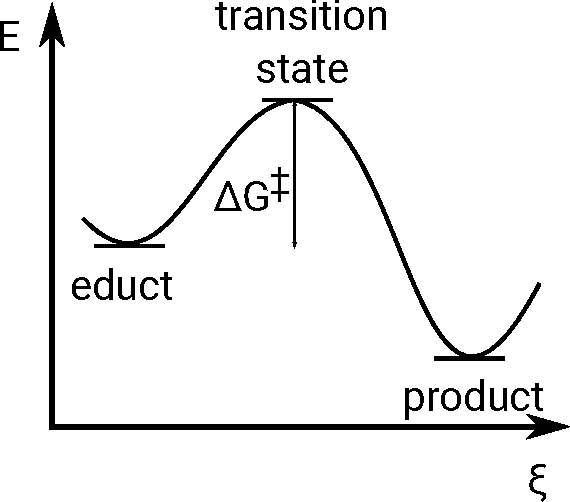
\includegraphics[width=0.4\textwidth]{figures/theory/MEP.pdf}
   \caption{Schematic view of a minimum energy path (MEP) for a thermal reaction.
The free energy $\Delta$G$^\ddagger= \Delta G_\textrm{TS}-\Delta G_\textrm{educt}$ for the reaction is also plotted.}
            \label{abb:mep}
\end{figure}


% One of the most prominent and widely used theories describing the transition state and the rate constants is Eyring theory of transition states.
% The most important approximations that are made are the following: i) there is an activated complex, ii) all particles that reached this complex/transition state will react towards the product.
% iii) At the transition state geometry, the motion along the reaction coordinate is seen as a one dimensional process and can be separated from all other degrees of freedom and can be seen as a translation.
% \\
% The equation for the rate constant is described by
% \begin{equation}\label{eyring}
% k(T)=\kappa\frac{k_BT}{h}e^{\Delta G^\ddagger(T)/(k_BT)},
% \end{equation}
% with the reaction rate constant $k$, Boltzmann's constant $K_B$, the temperature $T$, the difference of Gibb's free energy for the transition state and the educt $\Delta G^\ddagger$ and the transmission coefficient $\kappa$ that is a transmission coefficient (can be interpreted as a tunneling prefactor, for $\kappa>1$ tunneling occurs and for $\kappa<1$ non-classical reflection) tunneling corrections (seldomly applied in this work, not mention them here?), give the reaction rate constant as a function of temperature and barrier height.
% For the latter one needs to find the energies of the transition state and the educt.
% The educt geometry can simply be obtained by geometry optimization as a minimum on the PES.
% To find the transition state geometry and henceforth the energy we used Nudged Elastic Band calculations (NEB), with Climbing Image, Reaction path is approximated as a series of associated images, which are connected via spring forces.
% These spring forces prevent the images from optimizing into the local minimum next to the transition state.
% First a regular NEB, then on top of this climbing image was done which gives better convergence.
% In this calculation the energetically highest image is "optimized" towards higher energies in the contrary direction of the gradient.For the point found by this scheme we checked whether this is a transition state via frequency analysis, since a TST of first order has to have one imaginary mode that vibrates along the reaction path.
Transition state theory is a semi-classical theory: dynamics along the reaction coordinate $\xi$ are treated classically, but perpendicular directions allow for quantization of vibrational and rotational energy.
In thermodynamical equilibrium, all possible quantum states along the reaction coordinate are occupied with respect to their relative Boltzmann weight $P=e^{-\Delta E/(k_BT)}$ depending on the energy $E$ (or free energy $G$) and the temperature $T$.


Assuming the reaction
\begin{equation}
A+ B \rightleftarrows C^\ddagger \rightarrow D
\end{equation}
where reactants $A$ and $B$ are in thermodynamical equilibrium with the transition state $C^\ddagger$ and from this the reaction goes to the product $D$.
The rate constant can be determined with Eyring theory\cite{eyring,eyring-polanyi}:
\begin{equation}\label{eq:eyring}
k(T)=\kappa\frac{k_BT}{h}e^{-\Delta G^\ddagger(T)/(k_BT)}
\end{equation}
with the reaction rate constant $k(T)$, the transmission coefficient $\kappa$ which will be explained shortly, Boltzmann's constant $k_B$ and the difference of Gibb's free energy for the transition state and the educt $\Delta G^\ddagger = \Delta G_\textrm{TS} - \Delta G_\textrm{educt}$.
The equation gives the reaction rate constant as a function of temperature and free energy barrier height.
Note that this equation is only valid for cases where all reactands reaching the TS react to the product site.
No re-crossing is employed, so the rate is the upper limit in the classical picture.
For quantum effects, the rate can be increased due to tunneling, where reactants can overcome the barrier although they do not possess sufficient amount of energy for the barrier.
In order to account for this, the Eyring equation can be expanded with the transmission coefficient $\kappa$ which can be interpreted as a tunneling prefactor.
For $\kappa>1$ tunneling occurs and for $\kappa<1$ non-classical reflection or re-crossing to the educt side takes place.
\\\\

For the barrier height one needs to find the free energies of the transition state and the educt.
The educt geometry can simply be obtained by geometry optimization as a minimum on the PES.
Among different methods to find the transition state geometry and henceforth the energy we used Nudged Elastic Band calculations (NEB)\cite{Henkelman00a}, with Climbing Image\cite{Henkelman00b}.
This method approximates the reaction path as a series of associated images, which are connected via spring forces.
These spring forces prevent the images from optimizing into the local minimum next to the transition state.
First a regular NEB, then on top of this climbing image was applied which gives better convergence.
In this calculation the energetically highest image is "optimized" towards higher energies in the contrary direction of the gradient.
Any point found by this scheme must be checked whether it is a transition state via frequency analysis, since a TST of first order has to have one imaginary mode that vibrates along the reaction path.
Otherwise there is no transition state.

\section{Computational Details and Used Programs}
The majority of simulations/computations in this work were carried out using the Vienna \textit{ab initio} simulation package (VASP version 4 and 5.2)\cite{kresse1993,kresse2,kresse3,kresse4,kresse99}


For all the VASP calculations for the (0001) surface the parameters from prior work in the Saalfrank workgroup was used, because these were converged carefully by Dr. Jonas Wirth\cite{WirthJPCC2012,Wirth2014,Wirth2015,Wirth2016}.
Total energy convergence was achieved when energies between two SCF steps were smaller then $10^{-5}\,$eV and structures were assumed minima if the change in forces between two structures was below $0.01\,$eV/\AA{}.
The energy cutoff was set to $400\,$eV.
A vacuum gap of $26.4\,$\AA{} was used.


These parameters were adopted for the (11\=20) surface.
Here, the vacuum gap ranged from $17$ for the 10 layer slab to $11\,$\AA{} for the 25 layer slab, depending on the slab size in c-direction.
%the vacuum region is in the range of 17 Å for the 10 layer slab, 15 for the 15 layer slab, 13 for the 20 layer slab and 11 for the 25 layer slab
\\\\

The atom centered basis calculations with the programs CRYSTAL\cite{crystal14} (version 14) and the LMP2 calculations with cryscor\cite{cryscor} were not applied in our group before so no convergence test had been made so far.
The geometries and cell parameters from the VASP output were used as starting points and the usual convergence criteria of the programs were applied, convergence was achieved when energies between two steps were smaller than $2.7\times 10^{-6}\,$eV (with some exception when convergence was hard to achieve).
\\\\

Energy and MD plots shown in this work were prepared with gnuplot\cite{gnuplot}, surface structures and geometries were visualized with VMD\cite{vmd} and further illustrations were created with inkscape\cite{inkscape}.

\chapter{Water on $\upalpha$-Al$_2$O$_3$(11\=20)}

The (11\=20) surface of $\upalpha$-Al$_2$O$_3$ is not the most stable one under UHV conditions and was not studied so extensively so far.
Until now only a few experimental studies were performed for the (11\=20)-surface: X-ray reflectivity measurements by J. Catalano\cite{catalano}, who found that the surface is oxygen terminated and has two differently coordinated kinds of surface Al atom dimers.
LEED measurements by Becker \textit{et al.}\cite{Becker2002} showed a well defined $1\times 1$ diffraction pattern and found evidence that the surface is unreactive at room temperature with hydrogen.
The theoretical work of Marmier\cite{marmier} suggested that hydrogen is unreactive because the surface is fully hydroxylated at room temperature, even under UHV conditions.
In the work of Waychunas and coworkers\cite{sung} VSF spectra (vibrationally resonant sum frequency) were measured under ambient conditions (room temperature and air).
They found two different types of oxygen atoms on the surface, twofold and threefold coordinated ones.
It is assumed that the threefold coordinated will only be protonated under highly acidic conditions.
They also have evidence for molecularly adsorbed water on the surface.
However, all experimental studies\cite{catalano,sung,Becker2002} assume a high coverage situation, whereas this theoretical study is focused on the low-coverage regime.
With theoretical methods so far only the clean surface was studied by two different groups: Oshiyama \textit{et al.}\cite{kuri10} and Marmier\cite{marmier}.

\section{Surface Model}
To obtain the clean surface slab model of the (11\=20) surface a $2\times 2$ supercell was cut from the bulk.
The corresponding cell vectors were adopted from the bulk structure and a vacuum gap in z direction (perpendicular to the surface) was introduced to avoid unphysical interaction between the slabs in z direction.
In Figure \ref{abb:crystal_11-20}(a) the (11\=20) surface plane and the (0001) surface which is studied later in this work (Section \ref{sec:0001}) can be seen.
\begin{figure}[!h]
    \centering
    \subfigure[crystal]{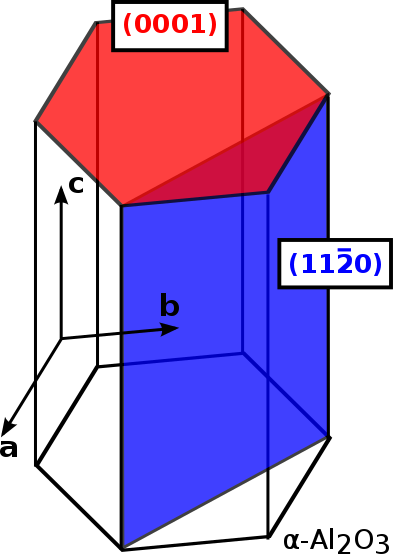
\includegraphics[width=0.30\textwidth]{figures/theory/al2o3-crystal.png}}
             \quad
             %add desired spacing between images, e. g. ~, \quad, \qquad, \hfill etc. (or a blank line to force the subfigure onto a new line)
    \subfigure[(11\=20), top view]{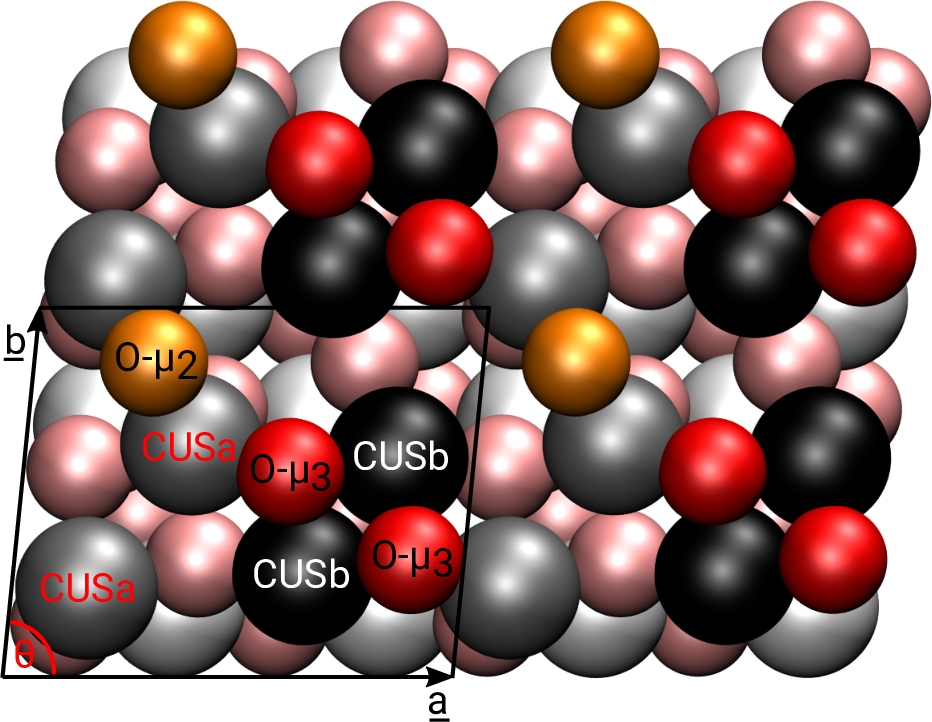
\includegraphics[width=0.58\textwidth]{figures/11-20/supercell_opt.png}}
             \quad
             %add desired spacing between images, e. g. ~, \quad, \qquad, \hfill etc. (or a blank line to force the subfigure onto a new line)
    \subfigure[(11\=20), side view]{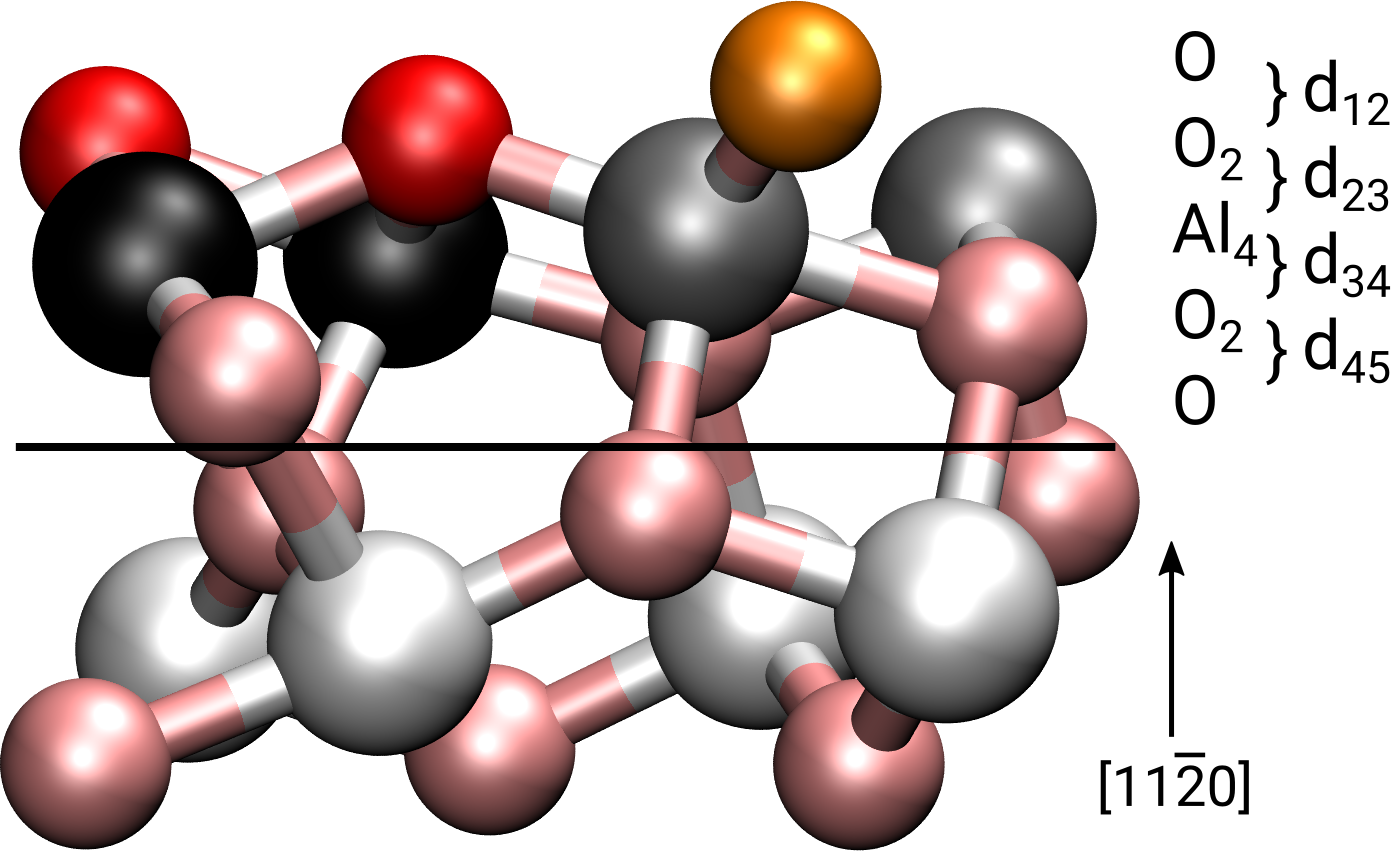
\includegraphics[width=0.5\textwidth]{figures/11-20/uc_opt.png}}
             \caption{The crystal cut of $\upalpha$-Al$_2$O$_3$, (a) schematic view compared to the (0001) surface, (b) a top view of the geometry optimized $2\times 2$ supercell with the nomenclature of the surface atoms.
The two types of surface Al atoms (grey CUSa and black CUSb) as well as the twofold and threefold coordinated oxygen atoms (orange O-$\mu_2$ and red O-$\mu_3$).
Subsurface atoms are indicated by pale colors.
(c) gives the side view of the unit cell showing the distinct atomic layers, again with the same color code as in (b).}
            \label{abb:crystal_11-20}
\end{figure}
Figure \ref{abb:crystal_11-20}(b) shows the top view and the cell vectors $\vec{a}$ and $\vec{b}$ of (11\=20).
They are not equal to those in the hexagonal cell for this particular surface cut, with $\vec{a}=10.36$\AA, $\vec{b}=14.16$\AA~ and $\vec{c}=20.5$\AA.
The angle $\theta$ between $\vec{a}$ and $\vec{b}$ is $84.56$\textdegree{} unlike the $60$\textdegree{} since the (11\=20) surface is tilted with respect to the top crystal plane.
The nomenclature and color code of the surface Al and O atoms is also shown: The Alumina atoms have the same number of oxygen neighbor atoms but differ slightly in the arrangement of their neighbors and the distance in the relaxed structure, whereas the oxygen atoms in fact differ by the number of neighbors.
The uppermost Al atoms are unsaturated and referred to as coordinatively unsaturates sites (CUS).
In this work, the grey spheres denote the CUSa atoms, the black ones depict the CUSb.
The twofold coordinated oxygen atoms (O-$\mu_2$) are shown in orange and the threefold coordinated (O-$\mu_3$) in red.
Atoms of the underlying layers are illustrated in pale colors, light grey for alumina and pale red for oxygen.


The unreconstructed unit cell consists of five atomic layers in z direction (O-O$_2$-Al$_4$-O$_2$-O), see Figure \ref{abb:crystal_11-20}(c)).
The spacing between these layers in the relaxed structure and in the bulk crystal is slightly changed as given in Table \ref{tab:layer-dist}.
The uppermost layer distance increases while it decreases for the deeper ones.
\begin{table}[!ht]
  \centering
 \caption{Distances between the top five layers (see also numbering in Figure \ref{abb:crystal_11-20}(c)) for different PBE+D2 optimized slab sizes ($3\times 3\times 1$ $\vec{k}$-point grid) and the unrelaxed bulk structure (right column) from theory.
All values are given in \AA.} 
\vspace*{.2cm}
\begin{tabular}{c|cccc|c}
\toprule
 & &\multicolumn{2}{c}{atomic layers}&&\\
    distance    & 10   & 15   & 20   & 25   &bulk \\\midrule
 d$_{12}$	&0.232 &0.234 &0.247 &0.245 &0.193 \\
 d$_{23}$	&0.642 &0.649 &0.638 &0.639 &0.741 \\
 d$_{34}$	&0.656 &0.655 &0.671 &0.672 &0.741 \\
 d$_{45}$	&0.198 &0.205 &0.209 &0.213 &0.191 \\\bottomrule
  \end{tabular}
  \label{tab:layer-dist}
\end{table}
A major issue of the optimization apart from layer spacing is that the interatomic distances of surface Al species change: the CUSa\textendash CUSa distance increases from $2.682$ to $2.994$\AA{}, the CUSa\textendash CUSb distance increased from $2.833$ to $2.876$\AA{} whereas the CUSb\textendash CUSb distance decreased from $2.682$ to $2.499$\AA{}.
The pairs of CUSa and CUSb can be interpreted as the Al dimers in the work of Catalano\cite{catalano}.


The supercell model that is used to a great extent in this work has ten atomic layers, with the lowest five fixed to the bulk value to mimic the surface situation.
For the calculations of the lattice vibrations up to 25 layers were considered (Figure \ref{abb:cell_sizes}).
For each slab size the respective lowest five layers were kept fixed, see chapter \ref{phonons}.
The spacing between the five top layers for each slab size is also displayed in Table \ref{tab:layer-dist}.


\begin{figure}[!h]
    \centering
    \includegraphics[width=0.90\textwidth]{figures/11-20/cell_sizes.pdf}
             \caption{Side view for the different cell sizes for 10, 15, 20 and 25 layers in z direction.
Surface atoms are shown in the color code clarified before.}
            \label{abb:cell_sizes}
\end{figure}
$\vec{k}$-points were sampled for five different grid sizes from $1\times 1\times 1$ to $5\times 5\times 1$.
In contrast to the even grid sizes, the odd ones contain the $\Gamma$-point and therefore are favorable.
It can be deduced from Figure \ref{abb:11-20-kpointsampling} that the $3\times 3\times 1$ grid is already converged with respect to the energy of the clean surface.
\begin{figure}[!h]
\centering
 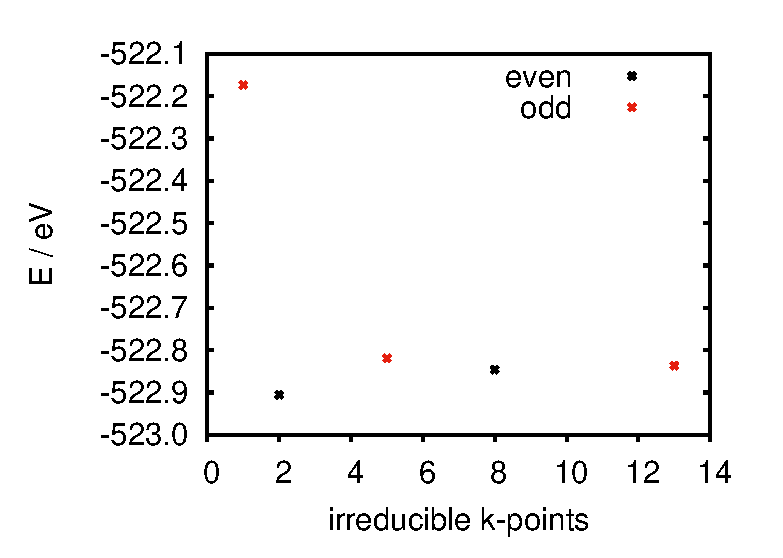
\includegraphics[width=0.7\textwidth]{figures/11-20/irreducibles-E.eps}
   \caption{PBE+D2 sampling of the $\vec{k}$-points, shown is the energy of the optimized supercell with respect to the number of irreducible $\vec{k}$-points.
The even values correspond to the $2\times 2 \times 1$ (2 irreducibles) and $4\times 4\times 1$ (8 irr.), whereas the odd, which contain the $\Gamma$-point, are described by $1\times 1\times 1$ (1 irr.), $3\times 3\times 1$ (5 irr.) and $5\times 5\times 1$ (13 irr.).}
            \label{abb:11-20-kpointsampling}
\end{figure}
\\

Starting from the $2\times 2$ supercell approach of the clean surface there are 16 CUS Al-atoms.
These have fewer bonds than the aluminum atoms in the bulk structure since the surface layer is  depleted.
These atoms are very interesting for adsorbate molecules/atoms, because these surface atoms are electron rich and can be addressed for adsorption.
Theoretically, these 16 atoms could be covered with water to gain 1 mono layer (ML).
Of these 16 CUS atoms eight are CUSa and eight CUSb.
On top of CUSb, a water molecule/OH residue can adsorb, but on top of a CUSa the adsorbate roams to a bridging inter-CUSa position between two CUSa.
Thus, the number of potential adsorbates is decreased to twelve forming 1ML.

\section{Structure Search}\label{structure_search11-20}
To study water adsorption, first a low coverage regime was investigated: One water molecule per $2\times 2$ supercell, which equals a coverage of 1/12.
For this a water molecule was put at different positions on the surface and relaxed.
By doing this one molecular minimum and several dissociated species including both CUS and oxygen types were found.
The multitude of different surface atoms gives rise to a large variety of possible adsorption geometries for the next neighboring situation (OH and H residue are adsorbed on two neighboring surface atoms) that even can be expanded when considering adsorbate structures with greater distance between the residues.
Adsorption energies and Gibb's free energy of the resulting next neighbor species can be seen in Table \ref{tab:ads_1water}.
The nomenclature for the adsorption sites which is used in the following gives at first the type of Al site where the OH-residue (we are not sure whether it is OH or OH$^-$) is adsorbed and at second place the oxygen type where the H(H$^+$) is adsorbed: OH site$\parallel$H site.
The term "inter" characterizes a position between two CUS atoms which leads to a bidentate adsorption pattern.
The additional notation with $^\prime$ denotes greater distances between the residues.
Direct neighbors do not have a $\prime$, the next neighbor structure is displayed by a single $\prime$, one position further $\prime\prime$ and the most distant position is $^\prime\prime\prime$ due to the periodic boundary conditions.
There is also one metastable molecular species that appears to be more stable than the found molecular minimum considering adsorption energy, but it cannot be classified as a stable minimum since there is one imaginary mode displaying the movement of the proton towards the dissociated species.


The adsorption energy is defined by Equation \ref{eq:Eads} as the energy of the adsorbed species compared to the energies of the clean surface and the free water molecule:
\begin{equation}\label{eq:Eads}
 E_\textrm{ads}=E_\text{ads. species}-(E_\text{free water molecule}+E_\text{surface}).
\end{equation}

\begin{table}[!ht]
  \centering
 \caption{For molecular and (singly) dissociated water on $\upalpha$-Al$_2$O$_3$(11\=20) adsorption energies E$_\textrm{ads}$ and Gibb's free energies $G_\textrm{ads}$ for different temperatures are given in eV.
E$_\textrm{ads}$ was calculated from Equation \ref{eq:Eads} and G$_\textrm{ads}$ is defined analogously.
These results were obtained with PBE+D2.
The three most stable configurations are marked with bold letters.
\vspace*{.2cm} 
  }
  \begin{tabular}{cl|cccc}
  \toprule
   \multicolumn{2}{c|}{Adsorbed Species}  & $E_\text{ads}$ & $G_\text{ads, 130 K}$  &  $G_\text{ads, 300 K}$  & $G_\text{ads, 400 K}$ \\\midrule
\multirow{1}{*}{molecular} & CUSb          &   -1.78  &-1.60 & -1.51  & -1.46 \\\hline
 \multirow{6}{*}{dissociated} & \textbf{inter-CUSa$\parallel$O-$\mu_2$} & \textbf{-2.50} &-2.27 & -2.16 & -2.09 \\
  & inter-CUSa$\parallel$O-$\mu_3$ & -1.67 &-1.44 &-1.33 & -1.27 \\
  & \textbf{CUSb$\parallel$O-$\mu_2$} & \textbf{-2.28} & -2.12& -2.03 &-1.97  \\
 & CUSb$\parallel$O-$\mu_3$ & -1.19 &-1.05 &-0.98 & -0.95 \\%Cb3_other
 & \textbf{inter-CUSb$\parallel$O-$\mu_2$} & \textbf{-2.09} &-1.88 &-1.80 & -1.76 \\
 & inter-CUSb$\parallel$O-$\mu_3$ & -1.89 &-1.71 & -1.63 & -1.58 \\\bottomrule
  \end{tabular}
  \label{tab:ads_1water}
\end{table}
\begin{figure}[!ht]
 \centering
\subfigure[CUSb]{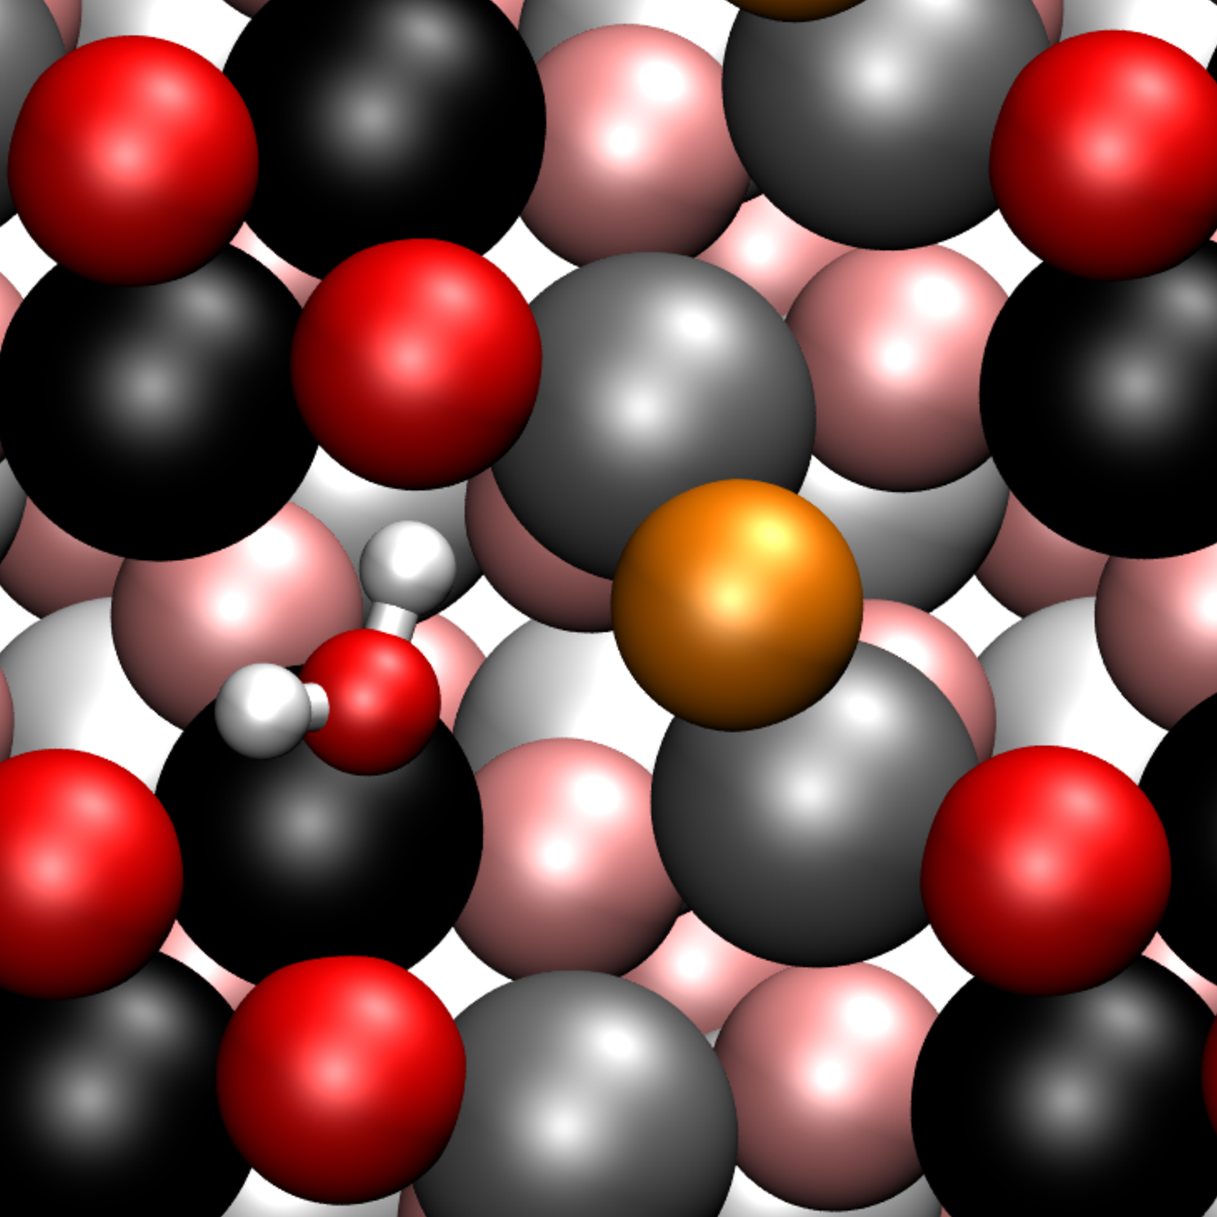
\includegraphics[width=0.2\textwidth]{figures/11-20/test-Cb.pdf}}
 \quad\quad
 \subfigure[inter-CUSa$\parallel$O-$\mu_2$]{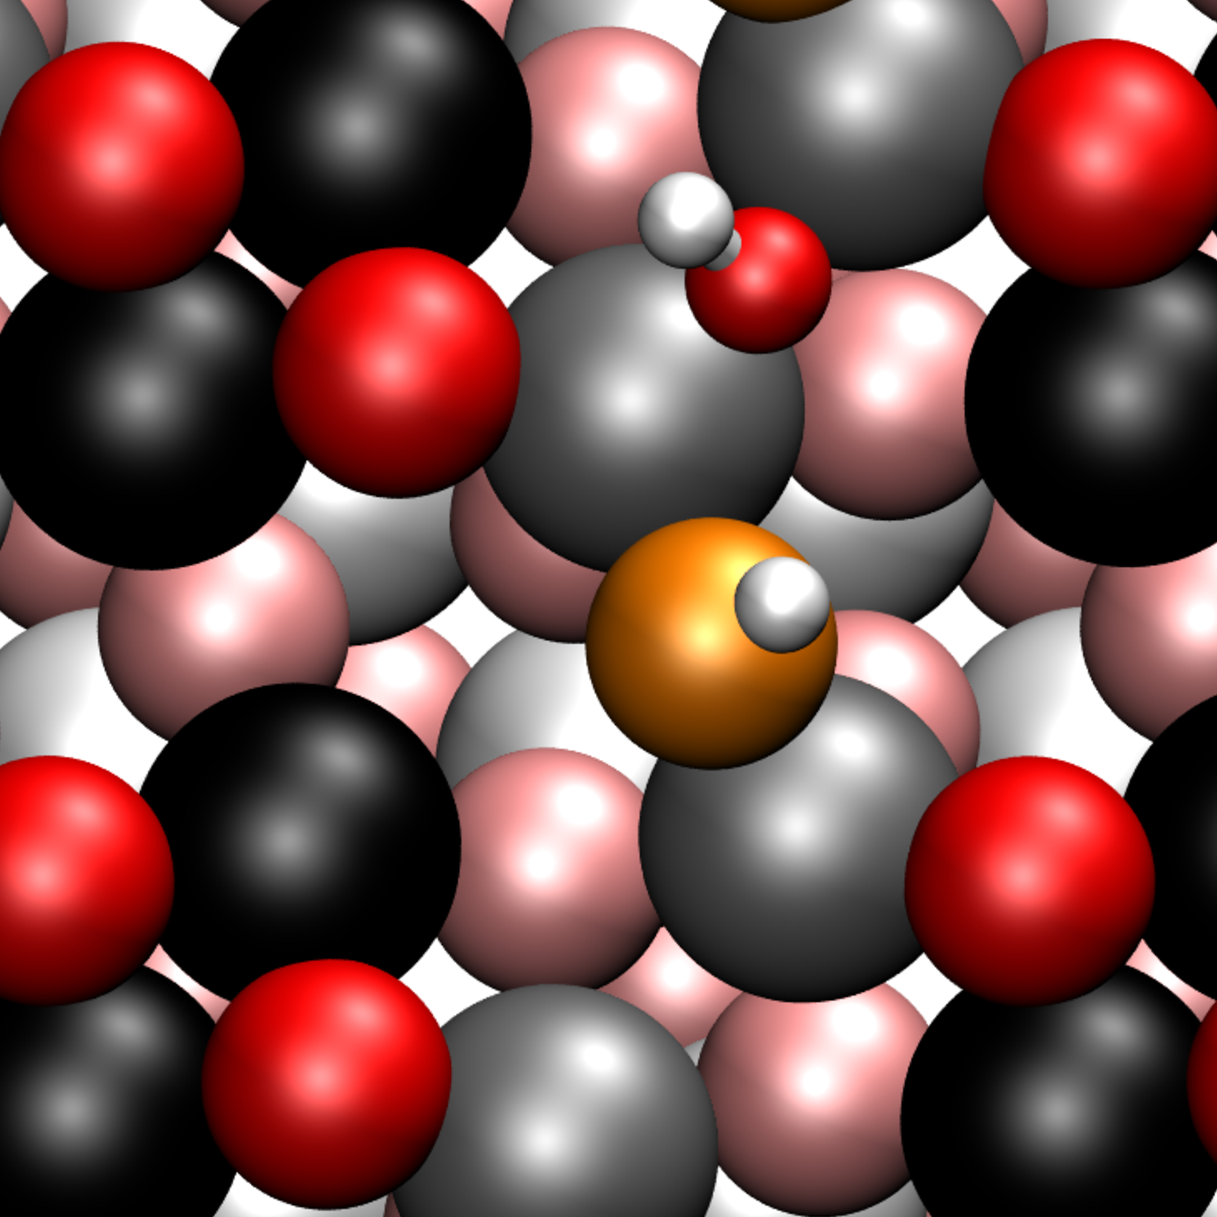
\includegraphics[width=0.2\textwidth]{figures/11-20/test-iCa2.pdf}}
  \quad
\subfigure[CUSb$\parallel$O-$\mu_2$]{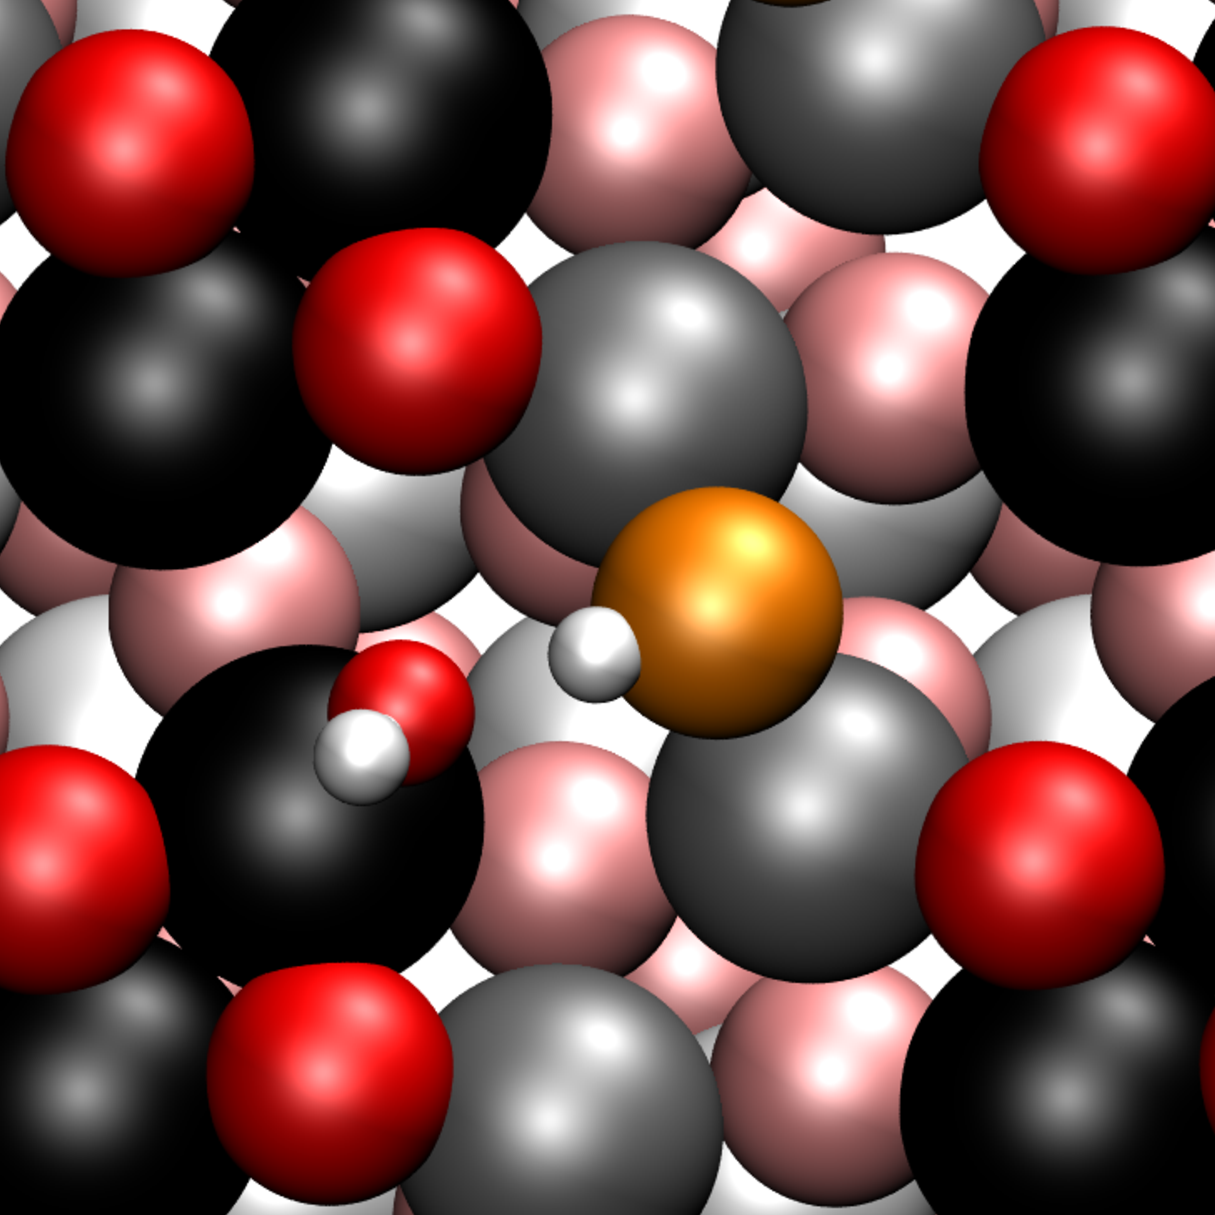
\includegraphics[width=0.2\textwidth]{figures/11-20/test-Cb2.pdf}}
 \quad
\subfigure[inter-CUSb$\parallel$O-$\mu_2$]{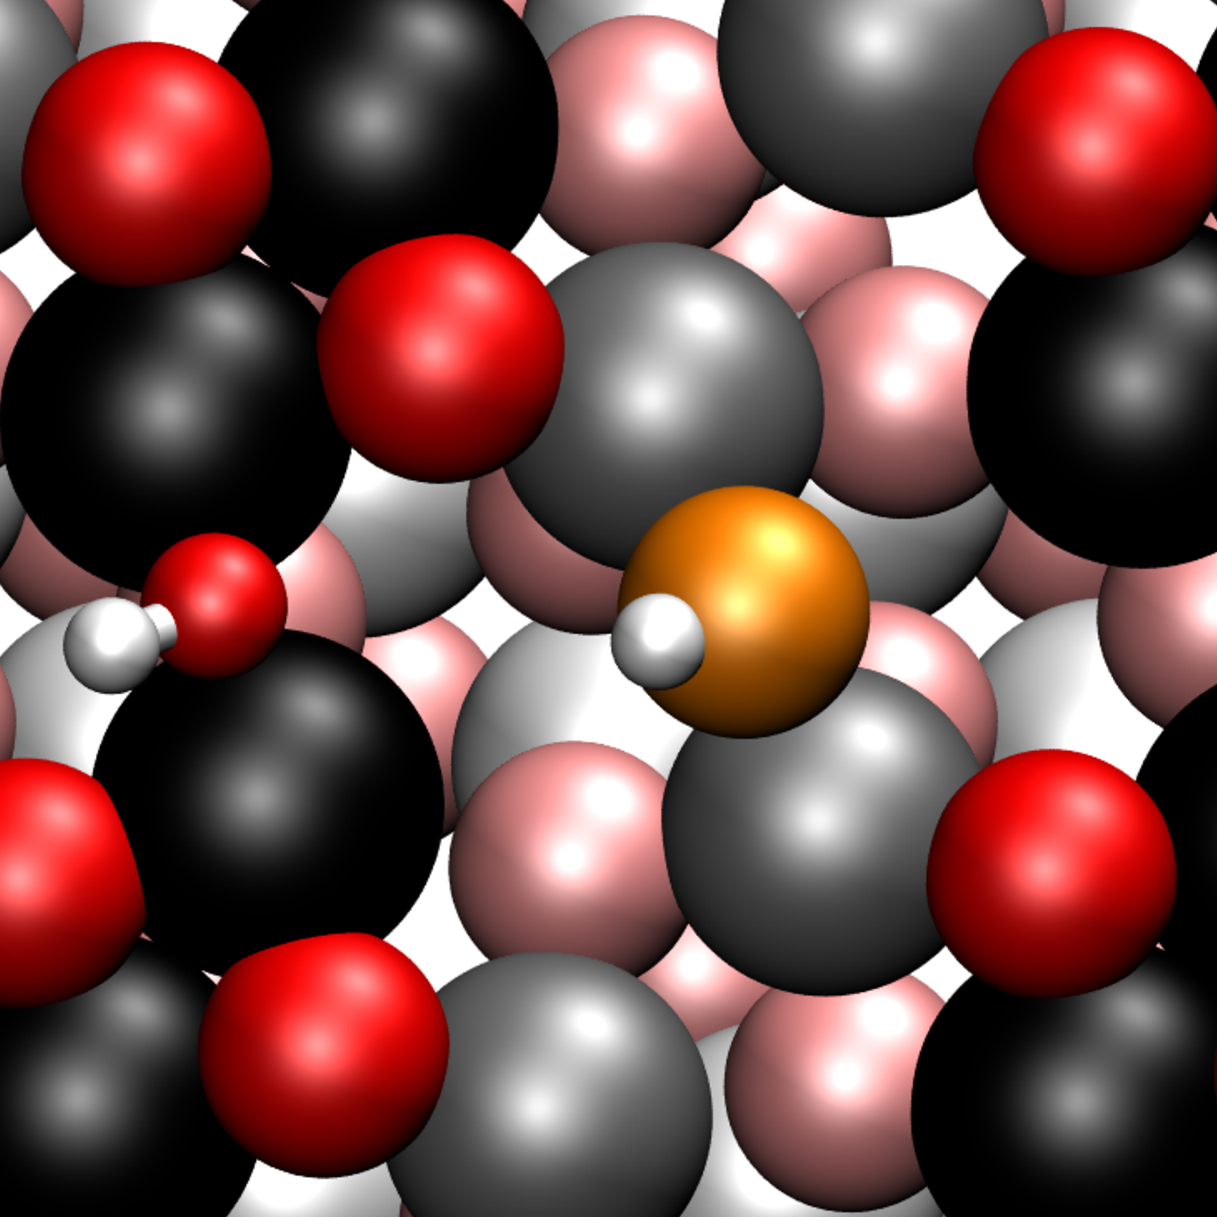
\includegraphics[width=0.2\textwidth]{figures/11-20/test-iCb2.pdf}}
\quad
\subfigure[inter-CUSa$\parallel$O-$\mu_3$]{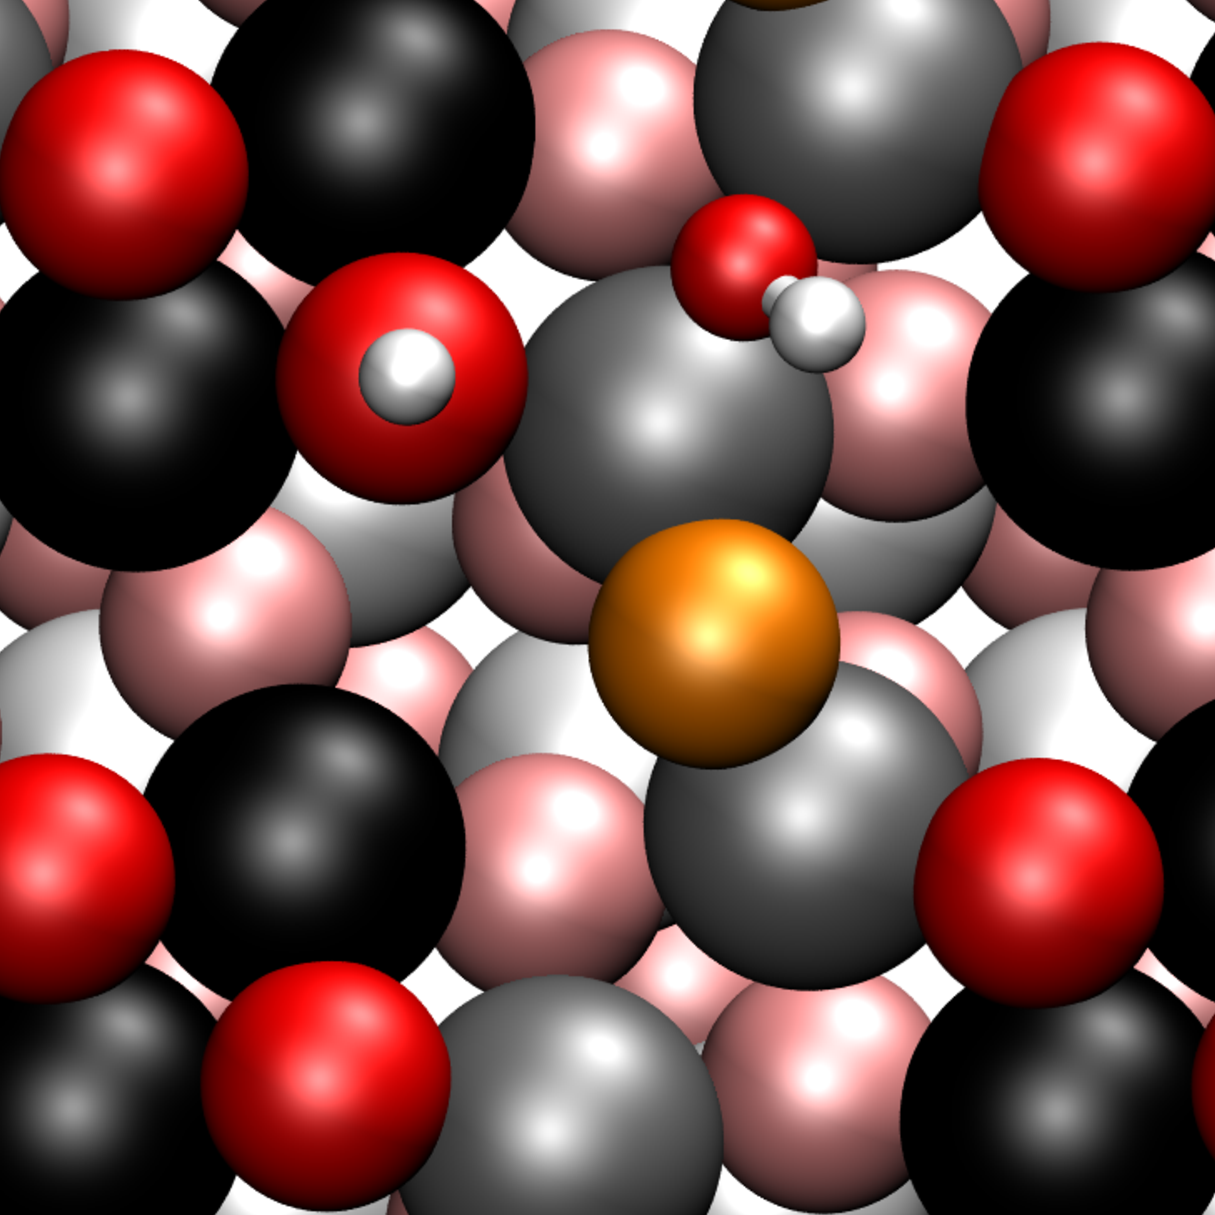
\includegraphics[width=0.2\textwidth]{figures/11-20/test-iCa3.pdf}}
 \quad
\subfigure[CUSb$\parallel$O-$\mu_3$]{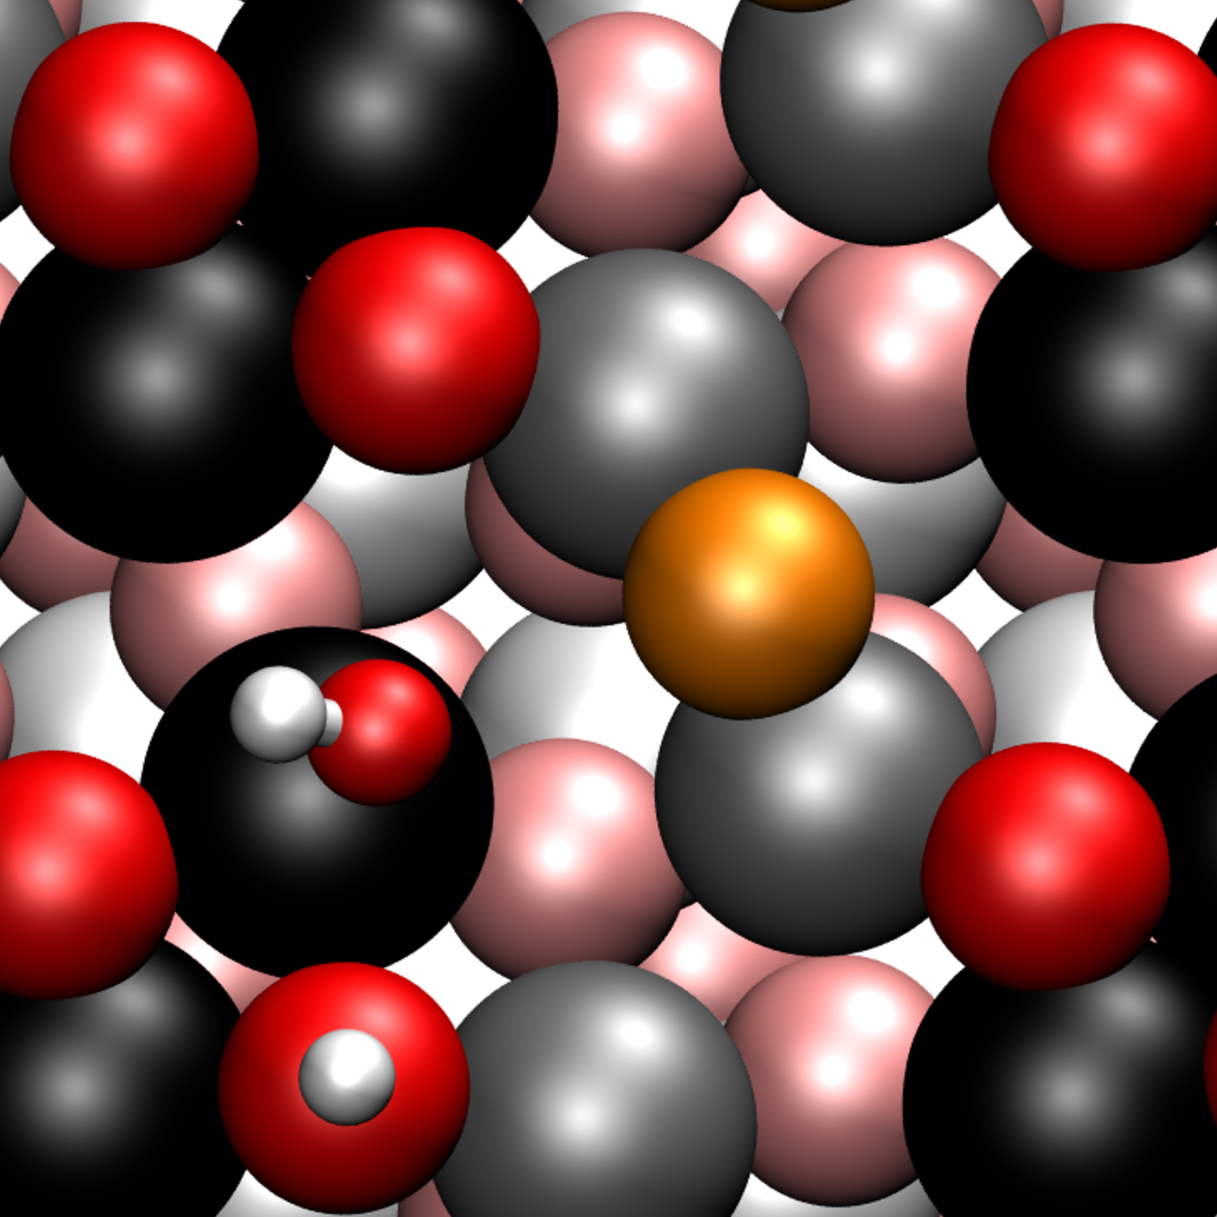
\includegraphics[width=0.2\textwidth]{figures/11-20/test-Cb3.pdf}}
 \quad
\subfigure[inter-CUSb$\parallel$O-$\mu_3$]{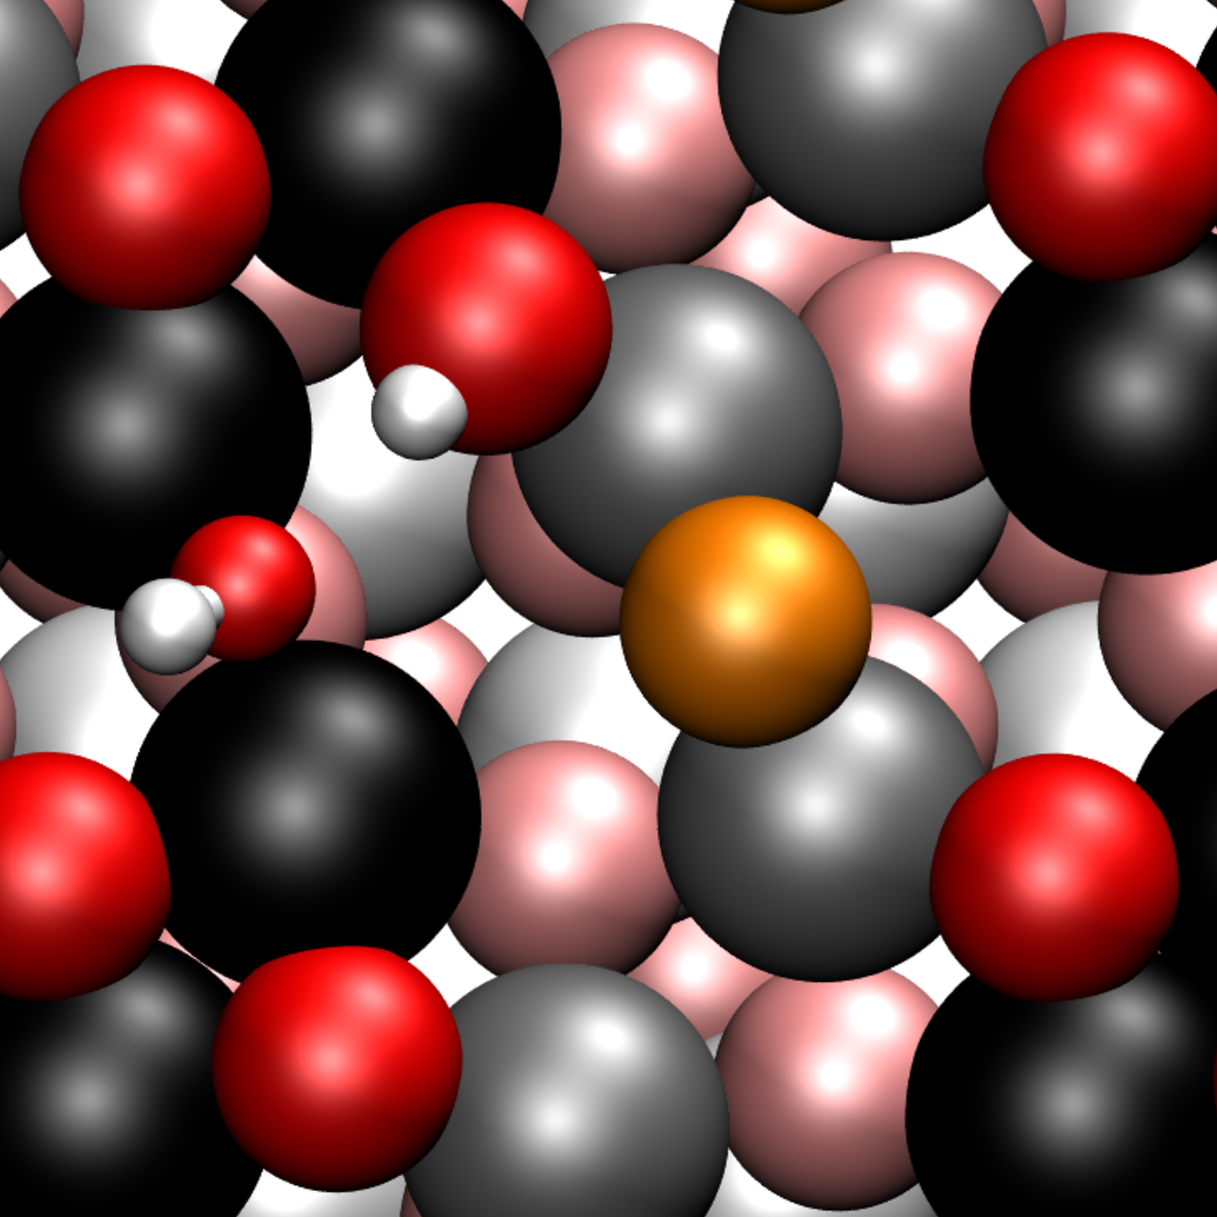
\includegraphics[width=0.2\textwidth]{figures/11-20/test-iCb3.pdf}}
 \caption{Top view of the adsorption geometries for molecular CUSb (a) and the next neighbor dissociated water 
((b)-(g)).
The color code is the same as in Figure \ref{abb:crystal_11-20}(b) and (c), CUSa grey, CUSb black, O-$\mu_2$ orange and O-$\mu_3$ red; Hydrogen is illustrated in white; the oxygen from water is in red but as a smaller sphere to make it distinguishable from the surface O atoms; subsurface layers are shown in pale colors.}
        \label{abb:ads-geoms}
 \end{figure}

The molecular minimum is substantially less stable than most of the dissociated species.
On the contrary, the dissociated water, where the twofold coordinated surface oxygen atom is addressed, is very stable, even in comparison to the more stable surface cuts (0001) and (1\=102) that were previously investigated in our group by Dr. Jonas Wirth\cite{Wirth2016,WirthJPCC2012}.
Dissociated species where the proton is located at a twofold coordinated surface oxygen are far more stable than the corresponding systems where the threefold coordinated oxygen is occupied.
This is due to the higher negative charge and the higher basicity of such twofold coordinated oxygen atom in comparison with the more saturated threefold coordinated O-$\mu_3$ oxygen atom.
In fact, the adsorption can be seen as a Lewis acid / base reaction\cite{Stair1981} with the Lewis acid character of the undercoordinated aluminum and the base character of the oxygen from the water molecule.


The adsorption of OH at an inter-CUSa site is more favorable than at a CUSb site, because the former corresponds to a site where in the bulk system another oxygen atom would be situated, which is not the case for the CUSb position.
Additionally, the CUSb position is electronically and sterically more hindered because of the two threefold coordinated oxygen atoms in the surroundings.


Dissociated species in direct neighborhood as shown in Table \ref{tab:ads_1water} and Figure \ref{abb:ads-geoms} are more stable than those where the proton and the OH-residue are further apart (see Table \ref{tab:ads_1waterfurther}), given the OH-residue has a stabilizing effect on the H and vice versa.
It is apparent from this table that the inter-CUSb$\parallel$O-$\mu_3^{\prime\prime\prime}$-species is more stable than the species inter-CUSb$\parallel$O-$\mu_3^{\prime\prime}$ (where the OH groups are closer to each other).
This is due to the fact that the periodic conditions actually lead to a decrease of the distance between OH groups in the former system.
The distances between the neighboring OH groups in the O-$\mu_3^{\prime\prime}$ system are $6.76$ and $7.71\,$\AA{}, compared to $9.34$ and $6.16\,$\AA{} in the O-$\mu_3^{\prime\prime\prime}$ system (the numbers refer to the two possible distance in the periodic system, direct and over the border of the unit cell).
The latter seems to be further away, but due to the periodic boundary conditions, one of the inter-adsorbate distances is smaller ($6.16$, compared to $6.76\,$\AA{}), which leads to the stabilization.

%one is in fact only slightly further away, the average distance is $0.739\,$\AA{} for inter-CUSb$\parallel$O-$\mu_3^{\prime\prime}$ and $0.780\,$\AA{} for inter-CUSb$\parallel$O-$\mu_3^{\prime\prime\prime}$.
% Although the distance is larger, there seems to be more stabilization by the surrounding surface atoms.
In Section \ref{reactions} dissociation and diffusion reactions will be given.
\begin{table}[!ht]
  \centering
 \caption{Comparison of adsorption energies for next neighbor dissociated species (without $^\prime$) and dissociated species where OH and H are further apart (with one, two or three $\prime$). 
Results for the adsorption energy E$_\textrm{ads}$ are given in eV.
\vspace*{.2cm} 
  }
  \begin{tabular}{cc}
  \toprule
  Adsorbed Species  & $E_\text{ads}$  \\\midrule
   inter-CUSa$\parallel$O-$\mu_3$ & -1.67 \\
   inter-CUSa$\parallel$O-$\mu_3^\prime$ & -1.42 \\\hline
   inter-CUSb$\parallel$O-$\mu_3$ & -1.89\\
   inter-CUSb$\parallel$O-$\mu_3^{\prime\prime}$ & -1.16\\
   inter-CUSb$\parallel$O-$\mu_3^{\prime\prime\prime}$ & -1.22\\\bottomrule
  \end{tabular}
  \label{tab:ads_1waterfurther}
\end{table}


Additionally, systems with additional atomic layers were studied.
The corresponding adsorption energies are shown in Table \ref{tab:eads_layers}.
Basically, the findings do not differ largely with increasing slab size.
The molecular species still is less stable than the O-$\mu_2$ dissociated species and is more stable than the O-$\mu_3$ dissociated ones (except for inter-CUSb$\parallel$O-$\mu_3$ dissociated system).
inter-CUSa$\parallel$O-$\mu_2$ is the most stable structure through all sampled systems sizes, inter-CUSb$\parallel$O-$\mu_2$ and CUSb$\parallel$O-$\mu_2$ change their stability (it approaches to nearly the same value for 25 layers) depending on the number of layers but still are some orders of magnitude less probable than inter-CUSa$\parallel$O-$\mu_2$.
Dissociated systems occupying the threefold coordinated surface oxygen atom remain in the same stability order.
%For higher quantity of layers, the inter-CUSb gets more favourable than CUSb, both for O-$\mu_2$ and O-$\mu_3$.
%This might be due to less interaction between neighboring oxygen atoms with the inter-CUSb adsorbed OH group.
\begin{table}[!ht]
  \centering
  \caption{Adsorption energies calculated from Equation \ref{eq:Eads} for molecular and dissociated species for different vertical slab sizes.
All values are given in eV.
The most stable systems (inter-CUSa$\parallel$O-$\mu_2$, CUSb$\parallel$O-$\mu_2$ and inter-CUSb$\parallel$O-$\mu_2$ are highlighted in bold letters.}
 \begin{tabular}{l|cccc}
 \toprule
 System                     & 10 layers& 15 layers& 20 layers&  25 layers \\\midrule
CUSb                                    &-1.78 &-1.80     &-1.81     &-1.83      \\\hline
\textbf{inter-CUSa$\parallel$O-$\mu_2$}    &\textbf{-2.50} &\textbf{-2.46} &\textbf{-2.54} &\textbf{-2.56}  \\
inter-CUSa$\parallel$O-$\mu_3$          &-1.67 &-1.67 &-1.78 &-1.80 \\
\textbf{CUSb$\parallel$O-$\mu_2$}          &\textbf{-2.28} &\textbf{-2.35} &\textbf{-2.36} &\textbf{-2.35} \\
CUSb$\parallel$O-$\mu_3$                &-1.19 &-1.71 &-     &-      \\
\textbf{inter-CUSb$\parallel$O-$\mu_2$}    &\textbf{-2.09} &\textbf{-2.43} &\textbf{-2.48} &\textbf{-2.36}  \\
inter-CUSb$\parallel$O-$\mu_3$          &-1.89 &-1.59 &-1.65 &-2.09 \\\bottomrule
\end{tabular}
\label{tab:eads_layers}
\end{table}
Table \ref{tab:eads_layers} shows that the most stable systems are already converged for the 10 layer slab with regard to adsorption energies (and also vibrational OD stretch frequencies as it will be seen in section \ref{nma}).


Furthermore, systems with a higher water coverage were considered, which offer the possibility to consider interaction between the adsorbate molecules. Some exemplary cases for two water molecules ($16.6\%$ coverage), four inter-CUSa$\parallel$O-$\mu_2$ ($33.3\%$ coverage) and a fully covered supercell (twelve molecules, $100\%$ coverage); for these systems normal mode analyses were carried out to get vibrational spectra, see Section \ref{phonons}.
Structures can be found in Figures \ref{abb:2water} and \ref{abb:4+fully}.
\begin{figure}[!ht]
 \centering
\subfigure[CUSb+CUSb$\parallel$O-$\mu_2$]{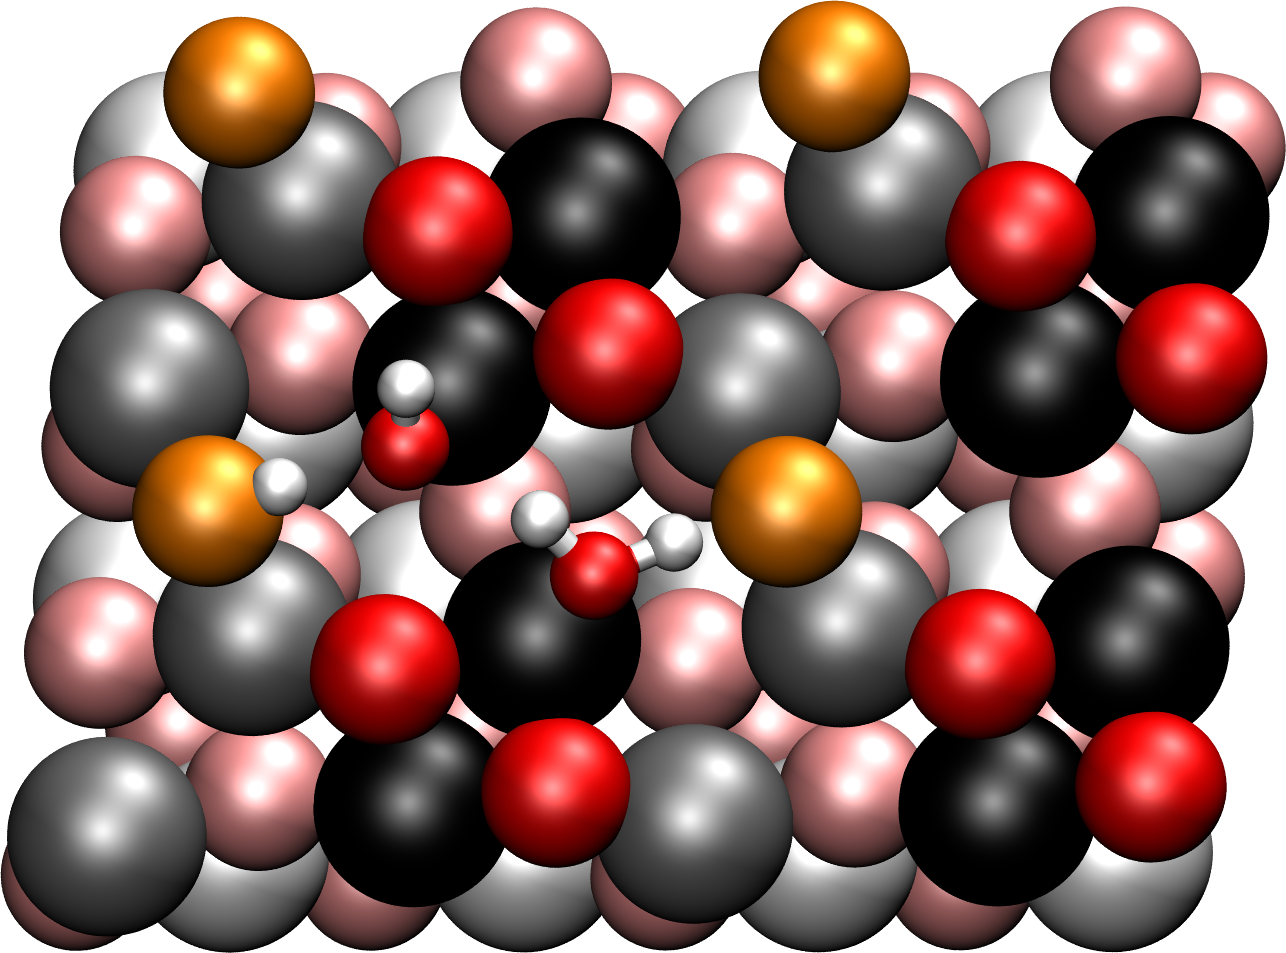
\includegraphics[width=0.302\textwidth]{figures/11-20/Cb-Cb2.png}}
 \quad\quad
 \subfigure[inter-CUSa$\parallel$O-$\mu_2$+CUSb$\parallel$O-$\mu_2$]{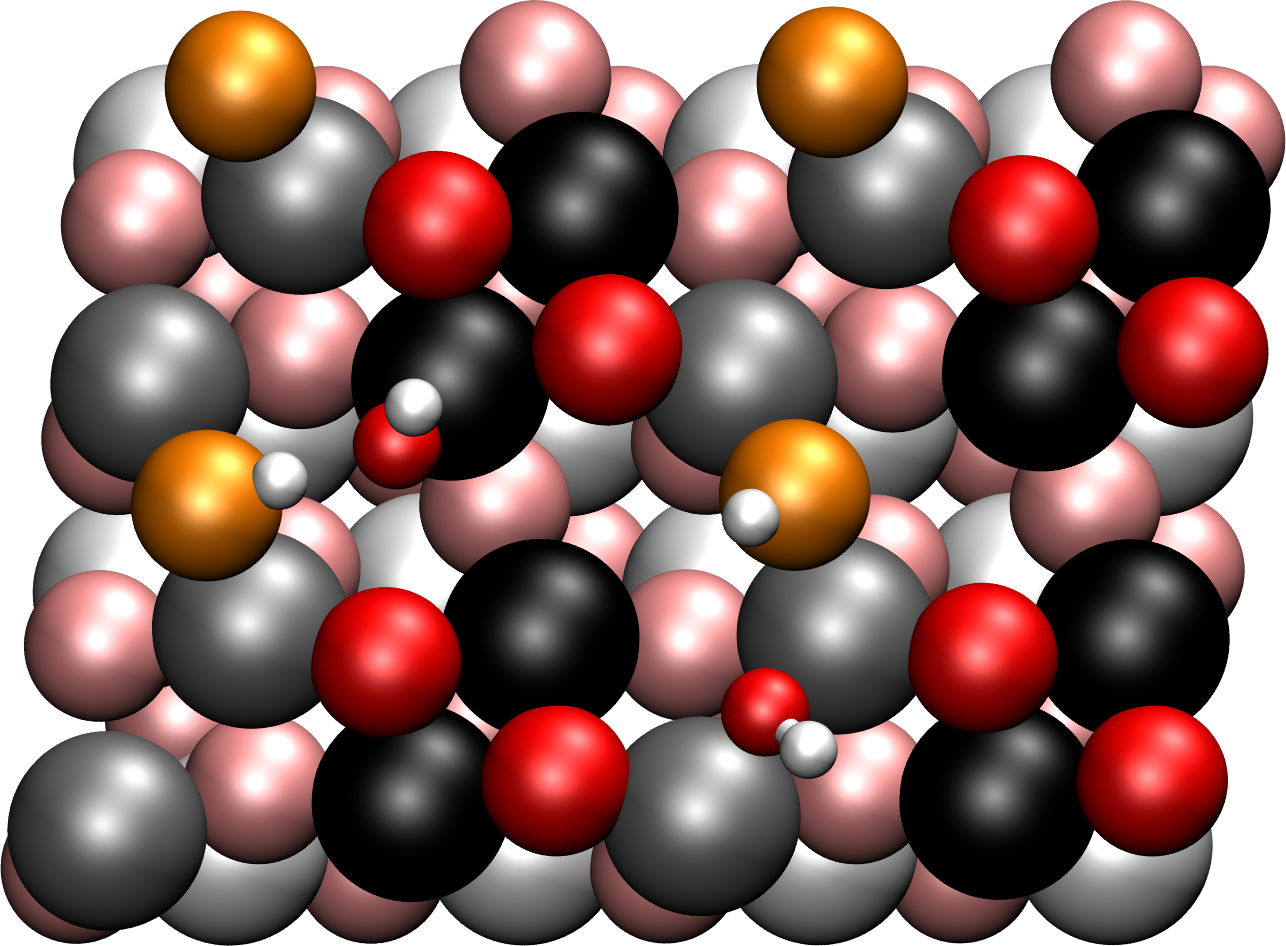
\includegraphics[width=0.304\textwidth]{figures/11-20/iCa2-Cb2.png}}
  \quad
\subfigure[2inter-CUSa$\parallel$O-$\mu_2$]{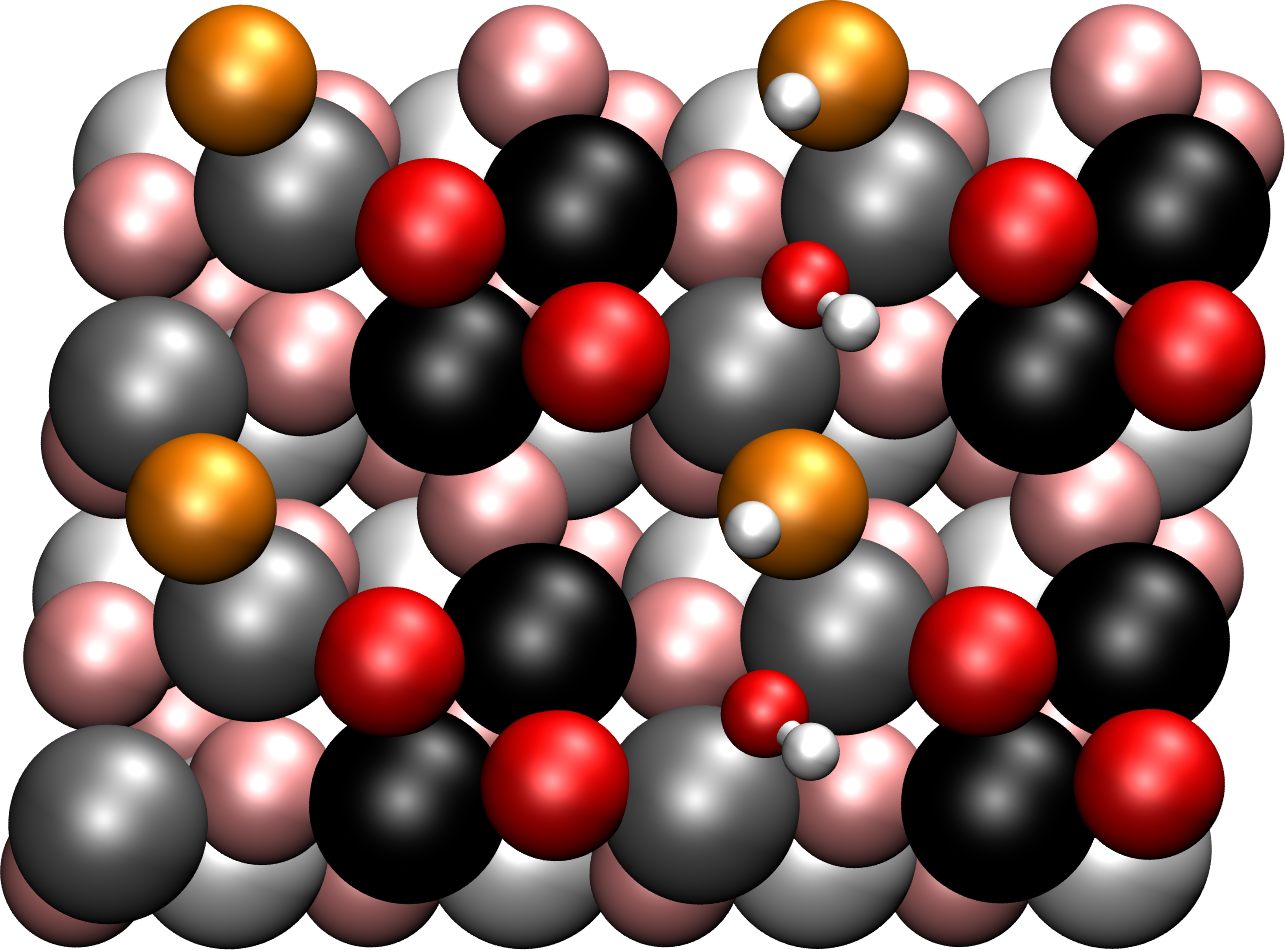
\includegraphics[width=0.302\textwidth]{figures/11-20/iCa2-iCa2.png}}
 \quad
 \caption{PBE+D2 optimized geometries of systems with two water adsorbates: (a) molecular CUSb and CUSb$\parallel$O-$\mu_2$, (b) the two most stable configurations inter-CUSa$\parallel$O-$\mu_2$ and CUSb$\parallel$O-$\mu_2$ and (c) 2 inter-CUSa$\parallel$O-$\mu_2$, which is the most stable adsorption pattern.}
        \label{abb:2water}
 \end{figure}
 \begin{figure}[!ht]
 \centering
\subfigure[4inter-CUSa$\parallel$O-$\mu_2$]{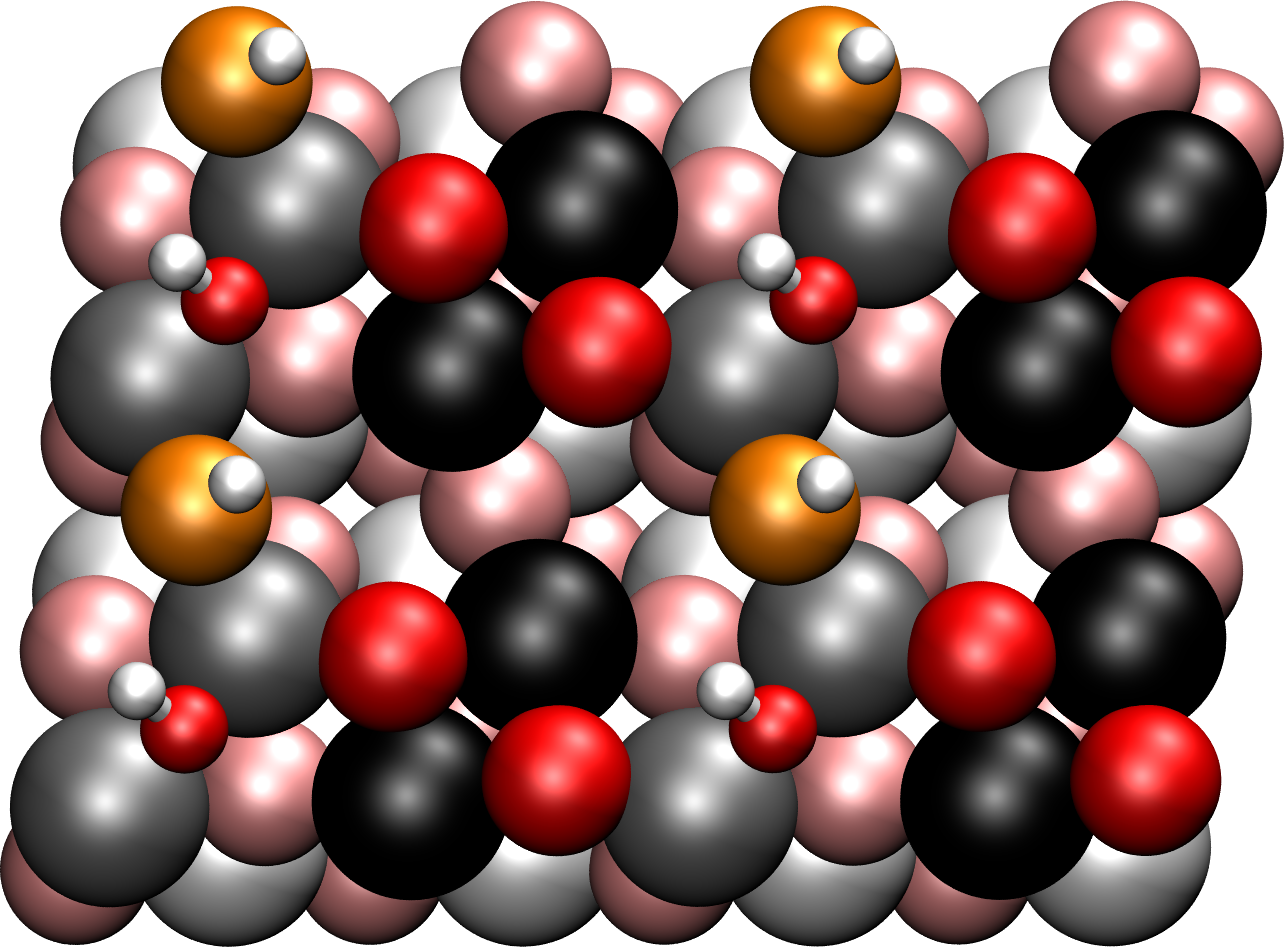
\includegraphics[width=0.4\textwidth]{figures/11-20/4iCa2.png}}
 \quad\quad
 \subfigure[1ML]{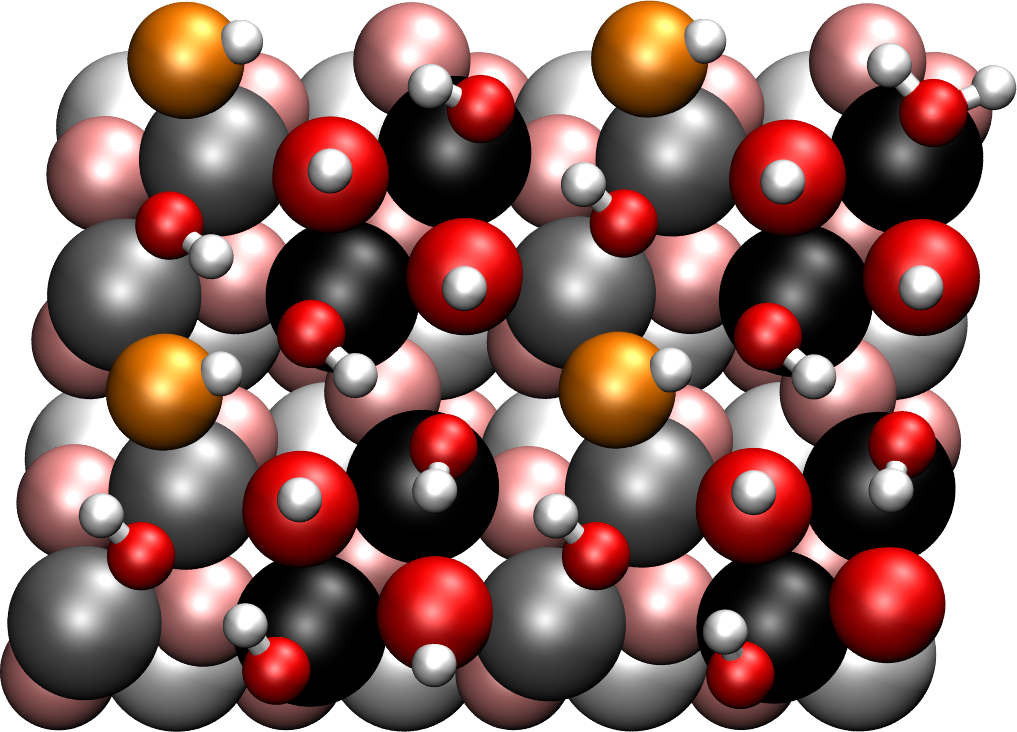
\includegraphics[width=0.4\textwidth]{figures/11-20/O-I-fully.png}}
 \caption{Optimized structures of the (a) 4inter-CUSa$\parallel$O-$\mu_2$ and (b) fully covered (1ML) system.
The latter one shows one molecular species and several hydrogen-bonded OH groups.}
        \label{abb:4+fully}
 \end{figure}

The stability of those species with $n$ adsorbed water molecules is defined as
\begin{equation}
 E_\textrm{ads}=E_\text{ads.
species}-(n\times E_\text{free water molecule}+E_\text{surface}).
\end{equation}
In Table \ref{tab:higher_water}, the adsorption energies for the high coverage species mentioned above are given.
\begin{table}[!ht]
  \centering
 \caption{Adsorption energies for higher water coverages in eV.
For better comparison in the third column labeled ``isolated species'' the summed energies for singly adsorbed water as given in Table \ref{tab:ads_1water} are presented.
\vspace*{.2cm} 
  }
  \begin{tabular}{lcc}
  \toprule
  Adsorbed Species  & $E_\text{ads}$ &isolated species \\\midrule
   CUSb(mol)+CUSb$\parallel$O-$\mu_2$ & -4.57 & -4.06\\
   inter-CUSa$\parallel$O-$\mu_2$+CUSb$\parallel$O-$\mu_2$ & -4.77 & -4.78\\
   2inter-CUSa$\parallel$O-$\mu_2$& -4.84 &-5.0 \\\hline
   4inter-CUSa$\parallel$O-$\mu_2$ & -9.55 & -10.0\\\hline
   12H$_2$O & -23.39& $^a$\tnote{a} \\   \bottomrule
  \end{tabular}
  \label{tab:higher_water}
  \begin{tablenotes}\footnotesize 
    \item[a] $^a$ In good approximation, there are 4 inter-CUSa-OD groups, 8 CUSb-OD groups, 8 O-$\mu_3$ and 4 O-$\mu_2$ OD groups, hence one can not calculate a sum of the isolated species.
  \end{tablenotes}
\end{table}
There are also the results for the higher coverages in comparison to results in the low coverage limit by adding them (see also column 3 in Table \ref{tab:higher_water}).
The structures where chosen exemplary such that the neighborhood effect shows three different outcomes: it can have a stabilizing effect, where the dissociated water stabilizes the molecularly adsorbed water in CUSb(mol)+CUSb$\parallel$O-$\mu_2$ (Figure \ref{abb:2water}(a)).
It can also have the contrary effect, as can be seen in the  2inter-CUSa$\parallel$O-$\mu_2$, which becomes less stable (Figure \ref{abb:2water}(c)).
On the other hand, there is the inter-CUSa$\parallel$O-$\mu_2$+CUSb$\parallel$O-$\mu_2$ which is merely affected by the neighboring OD residues (Figure \ref{abb:2water}(b)).
\\
\\

In experimental LEED data of the clean surface, the analysis of the data gave two sublattices, one of them can be clearly identified as the most stable O-I termination and the other one remains unidentified.
This unknown lattice could be a defect side or another surface termination but this suggestion could not be confirmed yet by experimental data since preparation and probing turns out to be difficult.
To pursue this thesis, a ``defect site'', the O-II terminated surface, as it is called in the nomenclature of Kurita\cite{kuri10}, was calculated.
This is the second most stable surface termination under most chemical potential conditions, mostly in Al-rich environment.
In this termination, the topmost oxygen layer of the O-I termination is missing.
As for the O-I termination, ten layers were considered and from these the lowest five layers were kept fixed to bulk values.
Both the clean surface and the fully covered ($1\,$ML) surface were optimized (see Figure \ref{abb:O-II-geom}) and frequency calculations were conducted, to obtain vibrational modes.
The structure of the clean surface, of course, differs by the ``missing'' oxygen O-$\mu_2$ atoms in the topmost layer, and the fully covered system is even more different: of twelve water molecules that can adsorb, seven adsorb molecularly and five dissociatively.
In comparison, the fully covered system for the O-I termination only shows one molecularly adsorbed molecule (\textit{cf.} Figure \ref{abb:4+fully}(b)).
 \begin{figure}[!ht]
 \centering
\subfigure[clean O-II surface]{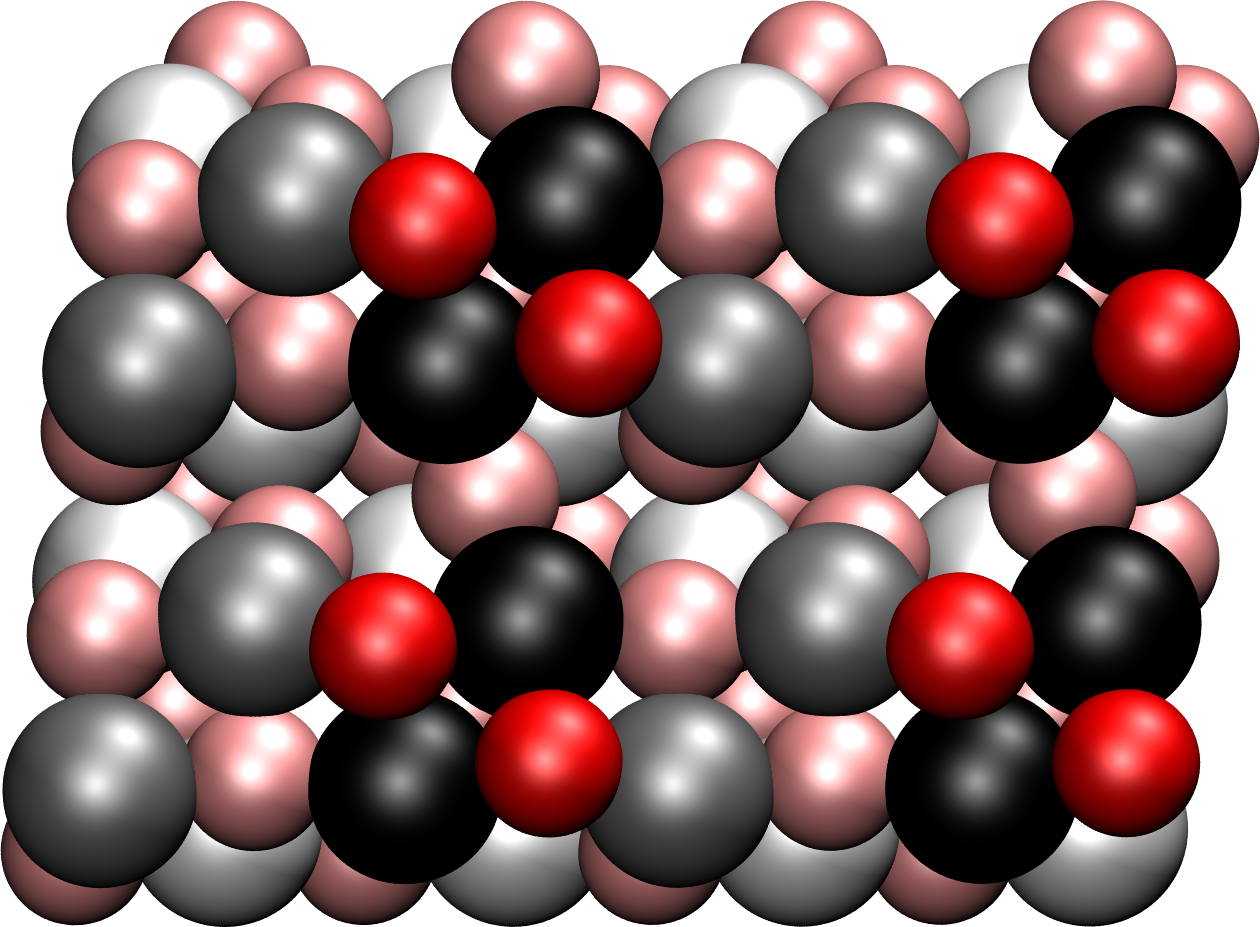
\includegraphics[width=0.4\textwidth]{figures/11-20/O-II-clean.png}}
 \quad\quad
 \subfigure[fully covered O-II surface]{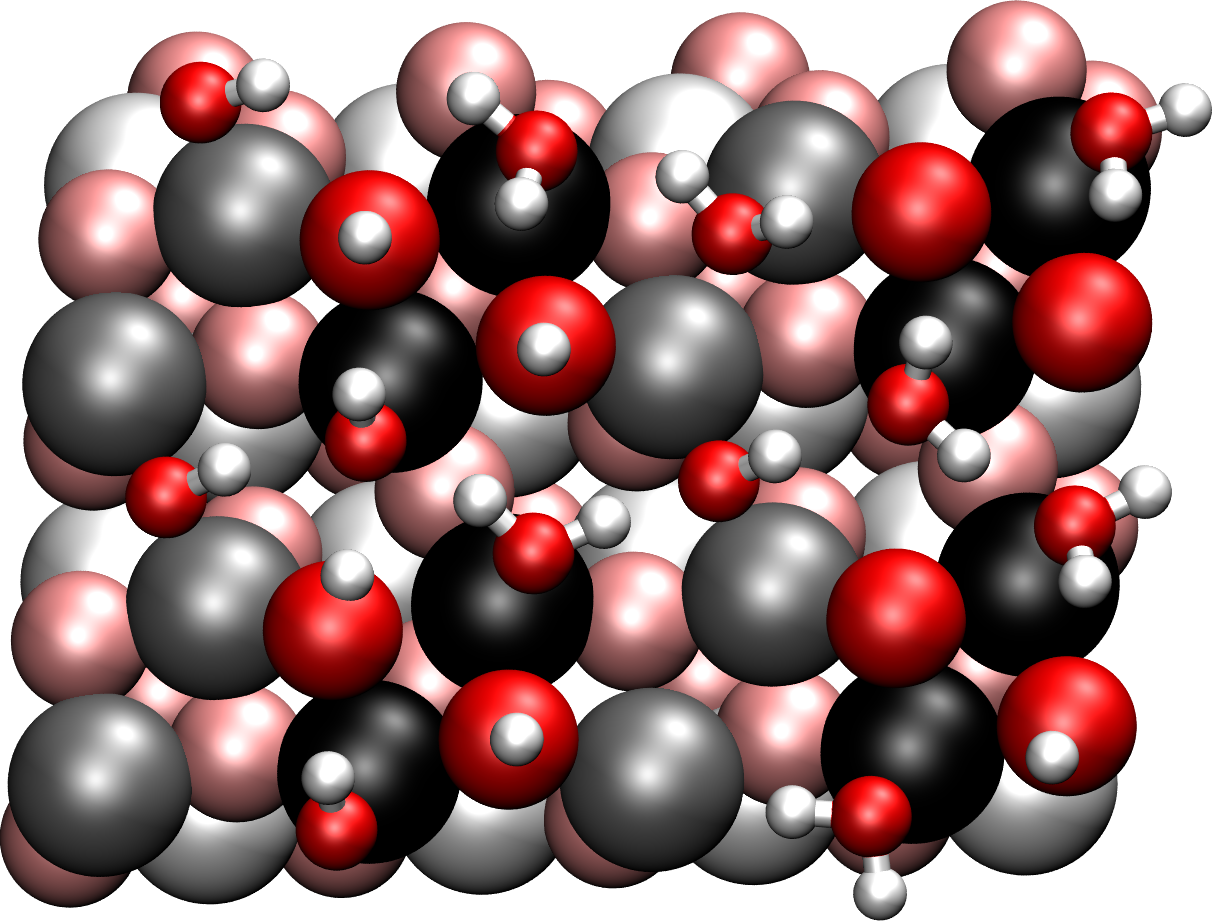
\includegraphics[width=0.4\textwidth]{figures/11-20/O-II-fully.png}}
 \caption{O-II terminated surface, as an example of a defect site optimized with PBE+D2.
The top layer oxygen atom from the O-I terminated surface is missing and gives rise to a different chemical behaviour.
(a) clean surface, (b) 1ML water adsorbed surface.}
        \label{abb:O-II-geom}
 \end{figure}

\section{Reactions and Microkinetic Model}\label{reactions}

Based on the minimum structures one has to identify reaction pathways to fully understand the reactivity of a system.
We utilize the NEB method including climbing image to search for transition states between the minima of the 10 layer slab.
We examined three different types of reactions: dissociation from the molecular minimum, as well as OH- and H-diffusion.
% These reaction paths and corresponding rates were calculated for hydrogen instead of deuterium that was used for vibrational frequencies since H$_2$O is more ubiquitous in nature (see Section \ref{sec:vib11-20}).
The dissociation reactions are named D, diffusion reaction Df-OH and Df-H, respectively, in Table \ref{tab:reaction-rates} and Figures \ref{mep} and \ref{mep2}.
In addition, molecular water diffusion on the surface is supposable but due to the low stability, it will dissociate before diffusion can occur.
In the publication that emerged from this work (Reference \cite{Heiden11-20_2018}) most of the reactions were introduced; additional reactions paths are also considered here.


We investigated five distinct dissociation reactions: the reactions from CUSb to the twofold coordinated oxygen (D-a) and one to the threefold coordinated O-$\mu_3$ (D-b).
One additional dissociation starts from the metastable inter-CUSa molecular structure that is, as said before, no minimum structure and goes to the most stable species inter-CUSa$\parallel$O-$\mu_2$ (D-c).
Two further dissociation reactions were converged but showed a two step process and are therefore not interesting in the first place (these reactions are CUSb$\rightarrow$inter-CUSa$\parallel$O-$\mu_2$ and CUSb$\rightarrow$inter-CUSb$\parallel$O-$\mu_2$ and both went via the dissociated CUSb$\parallel$O-$\mu_2$ intermediate).


As can be seen from Section \ref{structure_search11-20} (Table \ref{tab:ads_1water}), the molecular minimum CUSb has a lower stability compared to the O-$\mu_2$ dissociated minima.
The reaction D-a leads from the molecular minimum at CUSb to the twofold coordinated CUSb$\parallel$O-$\mu_2$:
 \begin{equation}
 \text{H$_2$O(CUSb)} \rightarrow \text{OH(CUSb)} + \text{H(O-$\mu_2$)} \tag{D-a}
      \label{dissa}
\end{equation}
The barrier is very low, about $0.002\,$eV as one can see from Table \ref{tab:reaction-rates} and Figure \ref{mep}(a), hence the reaction rate constant is very high, in the order of $k(\textrm{300\,K}=5.76\times 10^{12}\,$s$^{-1}$.
This low barrier might be due to the underestimation of barrier heights\cite{Zhao05} with the used functional PBE (compare section \ref{theorybeyond}).


For the other dissociation reaction D-b from CUSb to CUSb$\parallel$O-$\mu_3$, there is no barrier found at all with the applied method.
The reaction pathway shows simply an upgoing path in energy without any barrier (see Figure \ref{mep}(b)).
Thus, the reaction rate constant can only by approximated by using the product as a transition state to obtain $k(300\,K)=3.0\times 10^{13}$s$^{-1}$.
The molecular minimum is by $0.15\,$eV more stable than the dissociated structure on CUSb$\parallel$O-$\mu_3$.

\begin{equation}
  \text{H$_2$O(CUSb)} \rightarrow \text{OH(CUSb)} + \text{H(O-$\mu_3$)} \tag{D-b}
      \label{dissb}
\end{equation}
A further dissociation D-c from the metastable inter-CUSa species which is no confirmed minimum also shows no barrier (without Figure), assumingly because the educt  has a much lower stability than the product:
\begin{equation}
  \text{H$_2$O(inter-CUSa)} \rightarrow \text{OH(inter-CUSa)} + \text{H(O-$\mu_2$)} \tag{D-c}
      \label{dissc}
\end{equation}
It remains unclear whether this is due to the methodology and that the barrier is too low to be detected with the computational settings employed, or for other chemical reasons.


Besides dissociation, which is highly favored on this surface cut compared to more stable alumina surfaces\cite{Heiden11-20_2018}, diffusion reactions starting from the dissociated species are important for understanding further processes.
The OH diffusion reaction, Df-OH-a, moves from CUSb$\parallel$O-$\mu_2$ to the inter-CUSb position, which is relatively fast for OH diffusion reactions compared to the reactions at other alumina surfaces\cite{WirthJPCC2012,Wirth2016}.
\begin{equation}
 \text{OH(CUSb)} + \text{H(O-$\mu_2$)} \rightarrow \text{OH(inter-CUSb)} + \text{H(O-$\mu_2$)} \tag{Df-OH-a}
     \label{diffOHa}
\end{equation}
In this particular reaction, the OH residue diffuses from a CUSb position into a gap between two CUSb atoms (inter-CUSb position), where there is not much repulsion with neighboring surface oxygen atoms and other CUS atoms nearby during the diffusion, see Figure \ref{mep}(c).
Also the distance that has to be overcome is very small.
The barrier height equals $0.35\,$eV and the corresponding rate constant is $k(\textrm{300\,K})=1.88\times 10^6$s$^{-1}$.


In contrast to that the real CUS-to-CUS diffusion reaction, Df-OH-b, is much slower.
It is a diffusion from CUSb to inter-CUSa with the hydrogen residue staying at an O-$\mu_2$ position (see Figure \ref{mep}(d)).
This barrier of $1.07\,$eV is relatively high and leads to $k(\textrm{300\,K})=2.41\times 10^{-6}$s$^{-1}$.
\begin{equation}
 \text{OH(CUSb)} + \text{H(O-$\mu_2$)} \rightarrow \text{OH(inter-CUSa)} + \text{H(O-$\mu_2$)} \tag{Df-OH-b}
     \label{diffOHb}
\end{equation}
This is still faster than OH diffusion reaction for the alumina(0001) surface\cite{WirthJPCC2012,Wirth2014thesis}, where the rate constant of a comparable CUS-to-CUS diffusion reaction is $k(\textrm{300\,K})=4\times 10^{-45}$s$^{-1}$.
For the (1\=102) surface no OH diffusion was calculated, but the corresponding H$_2$O diffusion process is around $k(\textrm{300\,K})=1.4\times 10^{-3}$s$^{-1}$, and a comparable H$_2$O diffusion process for the (0001) surface has a rate constant of $k(\textrm{300\,K})=8\times 10^{-3}$s$^{-1}$.
For the (11\=20) surface no H$_2$O diffusion reactions can be observed due to the instability of the molecularly adsorbed species which would rather dissociate than diffuse.


A larger variety of reaction rate values can be achieved looking at hydrogen diffusion reactions.
The different types of surface oxygen atoms and also the distances between OH and H residues can affect the adsorption energy and the relative reaction kinetics.
As seen before, the hydrogen is preferably found on the twofold coordinated oxygen atom, but the reaction to a neighboring threefold coordinated oxygen is possible and opens the gate to structures with greater distance.
The reaction can take place with the OH residue being on a CUSb site:
\begin{equation}
 \text{OH(CUSb)} + \text{H(O-$\mu_2$)} \rightarrow \text{OH(CUSb)} + \text{H(O-$\mu_3$)} \tag{Df-H-a}
     \label{diffHa}
\end{equation}
The reaction is a proton transfer reaction with a barrier height of $\Delta E^\ddagger=0.94\,$eV and $k(300\,K)=4.53\times 10^{-3}$s$^{-1}$, but here the NEB transition state has no imaginary frequency so that no reliable rate can be derived, although the NEB path clearly shows a smooth barrier profile, compare Figure \ref{mep2}(a).
We assume that the point of maximum energy is very close to the transition state but not close enough for the frequency analysis to give one imaginary frequency.
 %investigate? is this normal/acceptable? MAYBE NOT MENTION IT AT ALL?


A further reaction, called Df-H-b, starting from the most stable inter-CUSa$\parallel$O-$\mu_2$ to the threefold coordinated oxygen can be seen in Figure \ref{mep2}(b):
\begin{equation}
 \text{OH(inter-CUSa)} + \text{H(O-$\mu_2$)} \rightarrow \text{OH(inter-CUSa)} + \text{H(O-$\mu_3^\prime$)} \tag{Df-H-b}
     \label{diffHb}
\end{equation}
The free energy barrier is $1.50\,$eV, giving a rate constant at $300\,$K of $4.90\times 10^{-13}$s$^{-1}$.
This process is so unlikely because a less favored O-$\mu_3$ position is occcupied and this position is also less stabilized because of the greater distance between OH$_{\text{surf}}$ and OH$_{\text{ads}}$ groups.
This reaction increases the distance to a position further away than next neighbor.
As mentioned before, the nomenclature for these structures uses primes ($\prime$) to display the distance.


A similar reaction can be seen in Figure \ref{mep2}(c) for the OH being situated on inter-CUSb and the hydrogen being adsorbed on an O-$\mu_2^{(\prime)}$ position, diffusing further away to O-$\mu_3^{\prime\prime}$, which is less stable:
\begin{equation}
 \text{OH(inter-CUSb)} + \text{H(O-$\mu_2^{(\prime)}$)} \rightarrow \text{OH(inter-CUSb)} + \text{H(O-$\mu_3^{\prime\prime}$)} \tag{Df-H-c}
     \label{diffHc}
\end{equation}
The free energy barrier is relatively high with $1.30\,$eV giving a rate constant $k(\textrm{300\,K})=9.96\times 10^{-1}$s$^{-1}$.
The $^\prime$ in the equation above is set in parantheses because it is the nearest possible O-$\mu_2$ position, but not the nearest possible distance from the OH$_\textrm{ads}$.

Going one step further from reaction Df-H-c, the following reaction leads to the position where OH and H have the greatest possible distance with the applied periodic bounding conditions:
\begin{equation}
 \text{OH(inter-CUSb)} + \text{H(O-$\mu_3^{\prime\prime}$)} \rightarrow \text{OH(inter-CUSb)} + \text{H(O-$\mu_3^{\prime\prime\prime}$)} \tag{Df-H-d}
     \label{diffHd}
\end{equation}
With an energy barrier of $0.94\,$eV the rate at $300\,$K is $1.1\times 10^{-3}$s$^{-1}$, see also Figure \ref{mep}(d).


These H diffusion paths can be assembled to a longer diffusion path leading from inter-CUSb$\parallel$O-$\mu_3$ to O-$\mu_2^\prime$ to O-$\mu_3^{\prime\prime}$ and to the furthest possible O-$\mu_3^{\prime\prime\prime}$.
An attempt to calculate the first reaction step was made but it did not converge for unknown reasons (not shown here).
The two next steps of this hydrogen migration path were studied (Df-H-c and Df-H-d).
The rate of the first step is unknown but it is assumed to be fast, because the product is a very stable O-$\mu_2$ configuration.
The second reaction (Df-H-c) has a rate of $10^{-1}$s$^{-1}$ which is a medium rate (not fast but also not slow).
The last step of this path is the slowest with a rate of $10^{-3}$s$^{-1}$.
% The corresponding adsorption energy profile is different from that: $-1.89$, $-2.09$, $-1.16$ and $-1.22$eV.
One can conclude that hydrogen migration in principle is possible but not likely because the O-$\mu_2$ acts as a trap for H that hinders further reactions.


\begin{table*}[ht]
  \centering
  \caption{Energy and free energy differences are given:  $\Delta E=E(\textrm{product}) - E(\textrm{educt})$, $\Delta E^{\ddagger}=E^\ddagger - E(\textrm{educt})$, respective for $G$.
Thermodynamic properties are given at $T=300\,$K.
$k$ is the rate constant from eq.~(\ref{eq:eyring}).
The three types of reactions are dissociation (D), OH diffusion (Df-OH) and H diffusion (Df-H).
``n.f.'' indicates ``not found''.
Numbers are given in italics if no barrier was confirmed or found.}
  \begin{tabular}{cl|cc|cc|c}
 \toprule
  \multicolumn{2}{c|}{\small{Reaction Type}}             & \small{$\Delta E$(eV)}& \small{$\Delta G(\textrm{300\,K})$(eV)} & \small{$\Delta E^{\ddagger}$(eV)} & \small{$\Delta G^{\ddagger}(\textrm{300\,K})$(eV)} & \small{$k(\textrm{300\,K})$(s$^{-1}$)}  \\\midrule
\multirow{3}{*}{\small{\ce{H2O} dissociation}} &
   \small{D-a}  & \small{-0.50} & \small{-0.52} & \small{0.01} & \small{0.002} & \small{5.76$\times 10^{12}$} \\
 & \small{D-b} & \textit{\small{0.59}} & \textit{\small{0.53}} & \textit{\small{0.15}} & \textit{\small{0.04}} & \textit{\small{3.0$\times$10$^{13}$}} \\
 & \small{D-c} &\textit{\small{-1.15}} &\textit{\small{-1.27}} & \small{n.f.} & \small{n.f.} & \small{n.f.}  \\\midrule
 \multirow{2}{*}{\small{OH diffusion}} &
   \small{Df-OH-a} & \small{0.19} & \small{0.22} & \small{0.35} & \small{0.39} & \small{1.88 $\times  10^6$}\\
 & \small{Df-OH-b}  & \small{-0.21} & \small{-0.13} & \small{1.07} & \small{1.10} & \small{2.41$\times 10^{-6}$} \\\midrule
\multirow{4}{*}{\small{H diffusion}} &
  \small{Df-H-a} &\textit{\small{0.76}} &\textit{\small{0.58}} & \textit{\small{0.94}}&\textit{\small{0.90}} & \textit{\small{4.53$\times$10$^{-3}$}}\\
& \small{Df-H-b}  & \small{1.08} & \small{1.04} & \small{1.65} & \small{1.49} & \small{4.90$\times 10^{-13}$} \\
& \small{Df-H-c} & \small{0.93} & \small{0.89} & \small{1.36} & \small{1.30} & \small{9.96$\times 10^{-10}$}\\
& \small{Df-H-d} & \small{-0.06} & \small{-0.07} & \small{1.05} & \small{0.94} & \small{1.05$\times 10^{-3}$} \\\bottomrule
  \end{tabular}
  \label{tab:reaction-rates}
\end{table*}

Proton diffusion reactions are much more variable than OH diffusions or dissociation reactions, providing reaction rates ranging from $10^{-13}$ to $10^{-3}$s$^{-1}$ at $300\,$K.
The barriers and therefore also rate constants for H-diffusion cover a wider range depending on two facts: the question whether O-$\mu_2$ or O-$\mu_3$ is occupied and the distance between the OH and H residues.


It was shown that reactions leading to another situation than next neighbored, increasing the distance between OH and H are less favorable since geometries with the residues further apart are energetically less stable (compare Table \ref{tab:ads_1waterfurther}).
\begin{figure*} [!ht]
\centering
\subfigure[D-a: CUSb $\rightarrow$CUSb$\parallel$O-$\mu_2$]{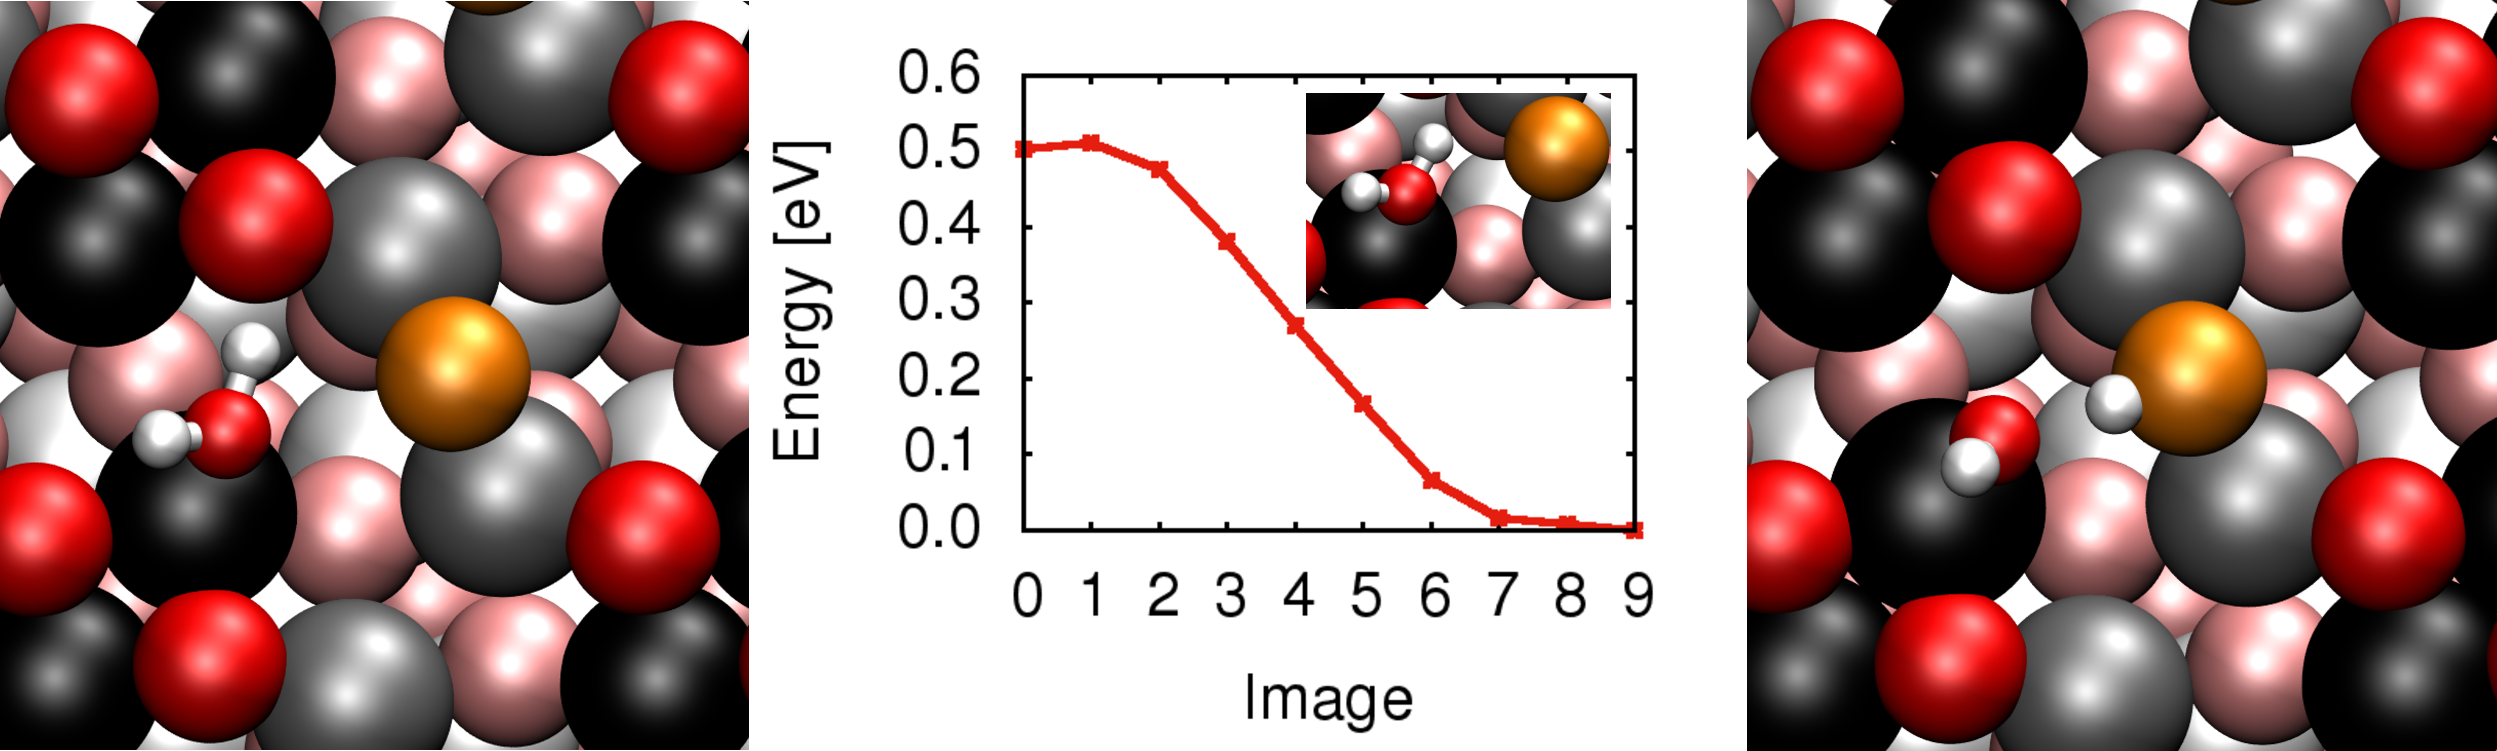
\includegraphics[width=0.9\textwidth]{figures/11-20/Diss_Cb-Cb2.pdf}}
         \quad
\subfigure[D-b: CUSb $\rightarrow$CUSb$\parallel$O-$\mu_3$]{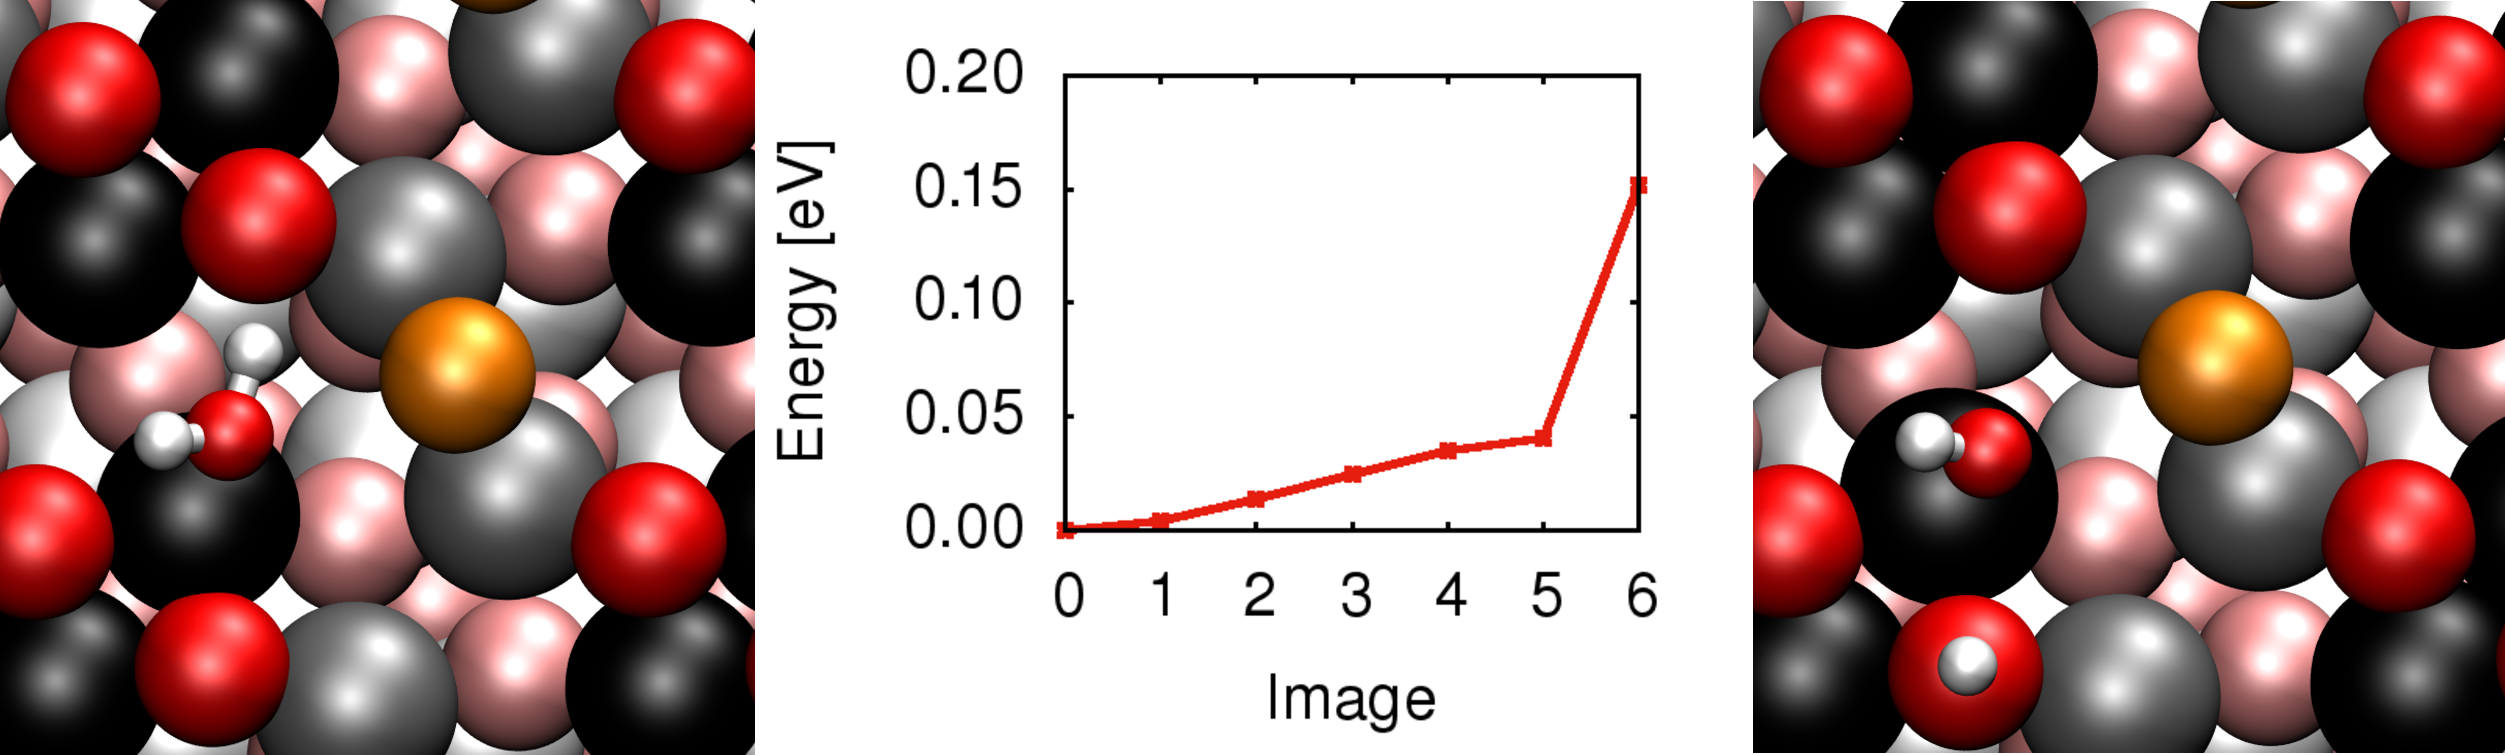
\includegraphics[width=.9\textwidth]{figures/11-20/Diss_Cb-Cb3.pdf}}
 \quad
\subfigure[Df-OH-a: CUSb$\parallel$O-$\mu_2$ $\rightarrow$inter-CUSb$\parallel$O-$\mu_2$]{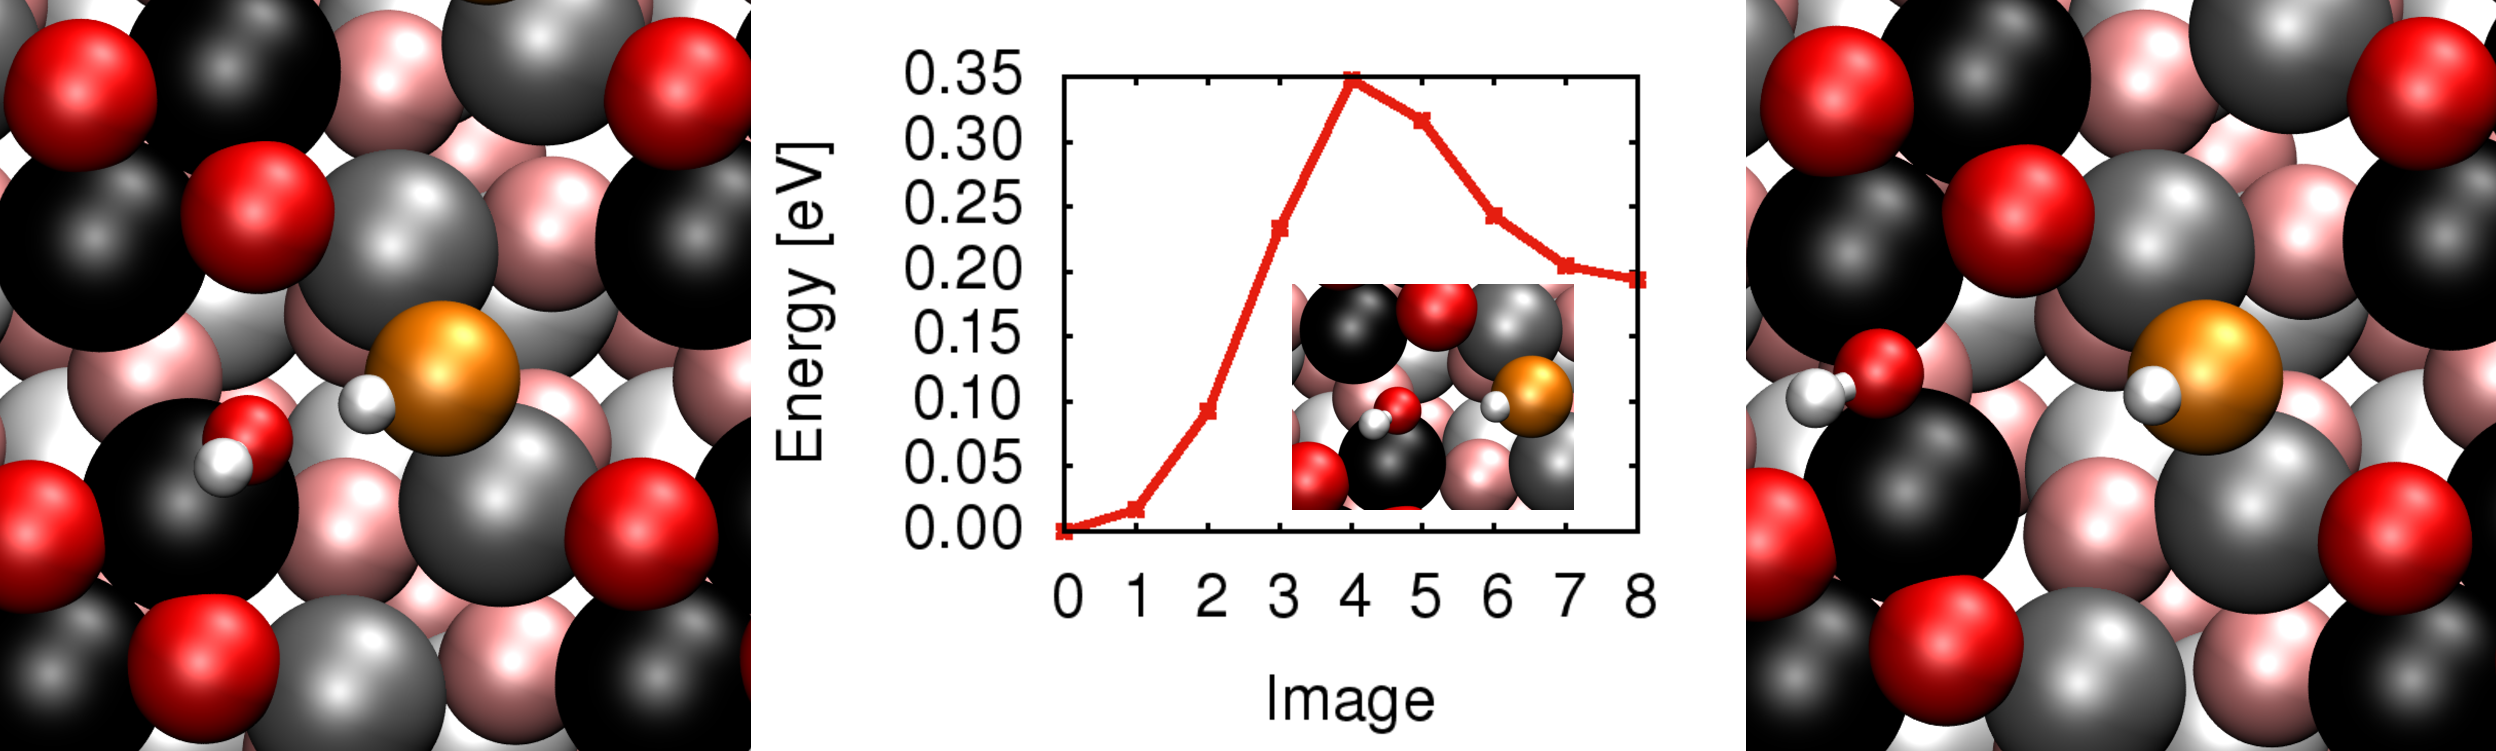
\includegraphics[width=.9\textwidth]{figures/11-20/Diff-OH_Cb2-iCb2.pdf}}
 \quad
\subfigure[Df-OH-b: CUSb$\parallel$O-$\mu_2$ $\rightarrow$inter-CUSa$\parallel$O-$\mu_2$]{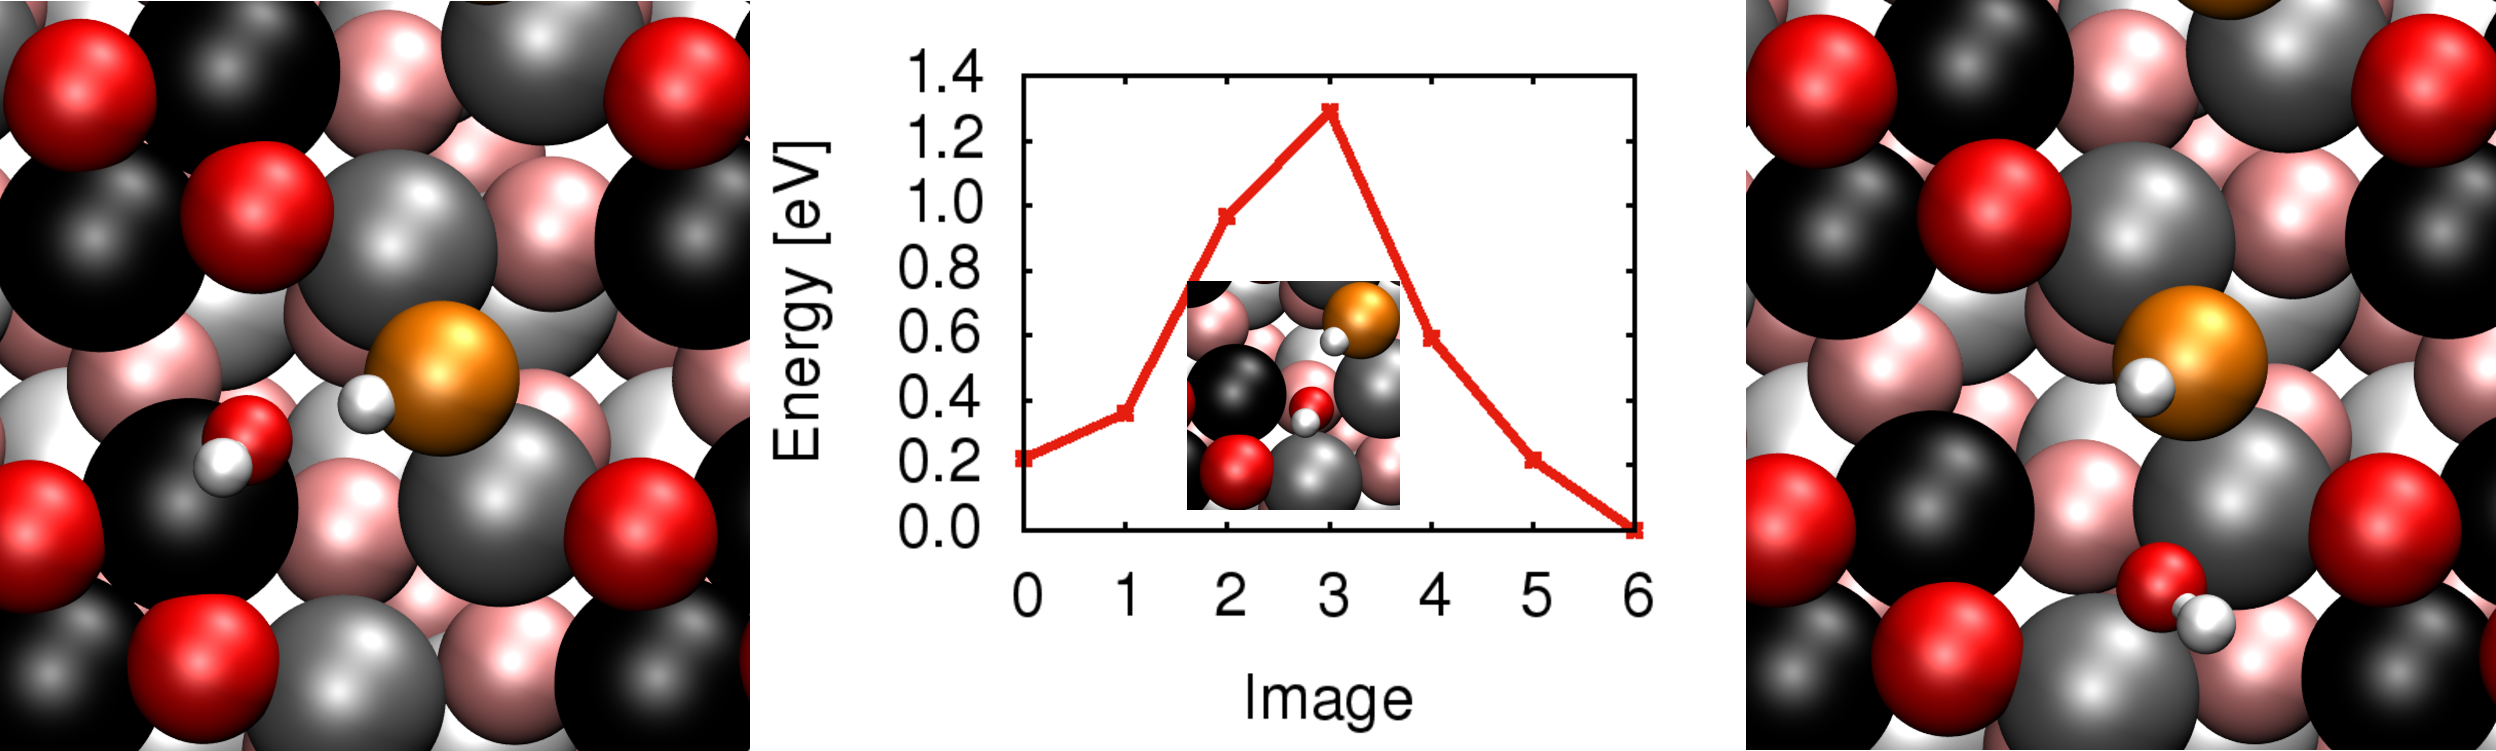
\includegraphics[width=.9\textwidth]{figures/11-20/Diff-OH_Cb2-iCa2.pdf}}
\caption{Minimum energy paths with transition states (inlay; if available), and both educt (left) and product (right) states for D-a, D-b, D-c, Df-OH-a and Df-OH-b reactions, respectively.
The color code is as explained above.}
       \label{mep}
\end{figure*}
\begin{figure*} [!ht]
\centering
\subfigure[Df-H-a: CUSb$\parallel$O-$\mu_2\rightarrow$CUSb$\parallel$O-$\mu_3$]{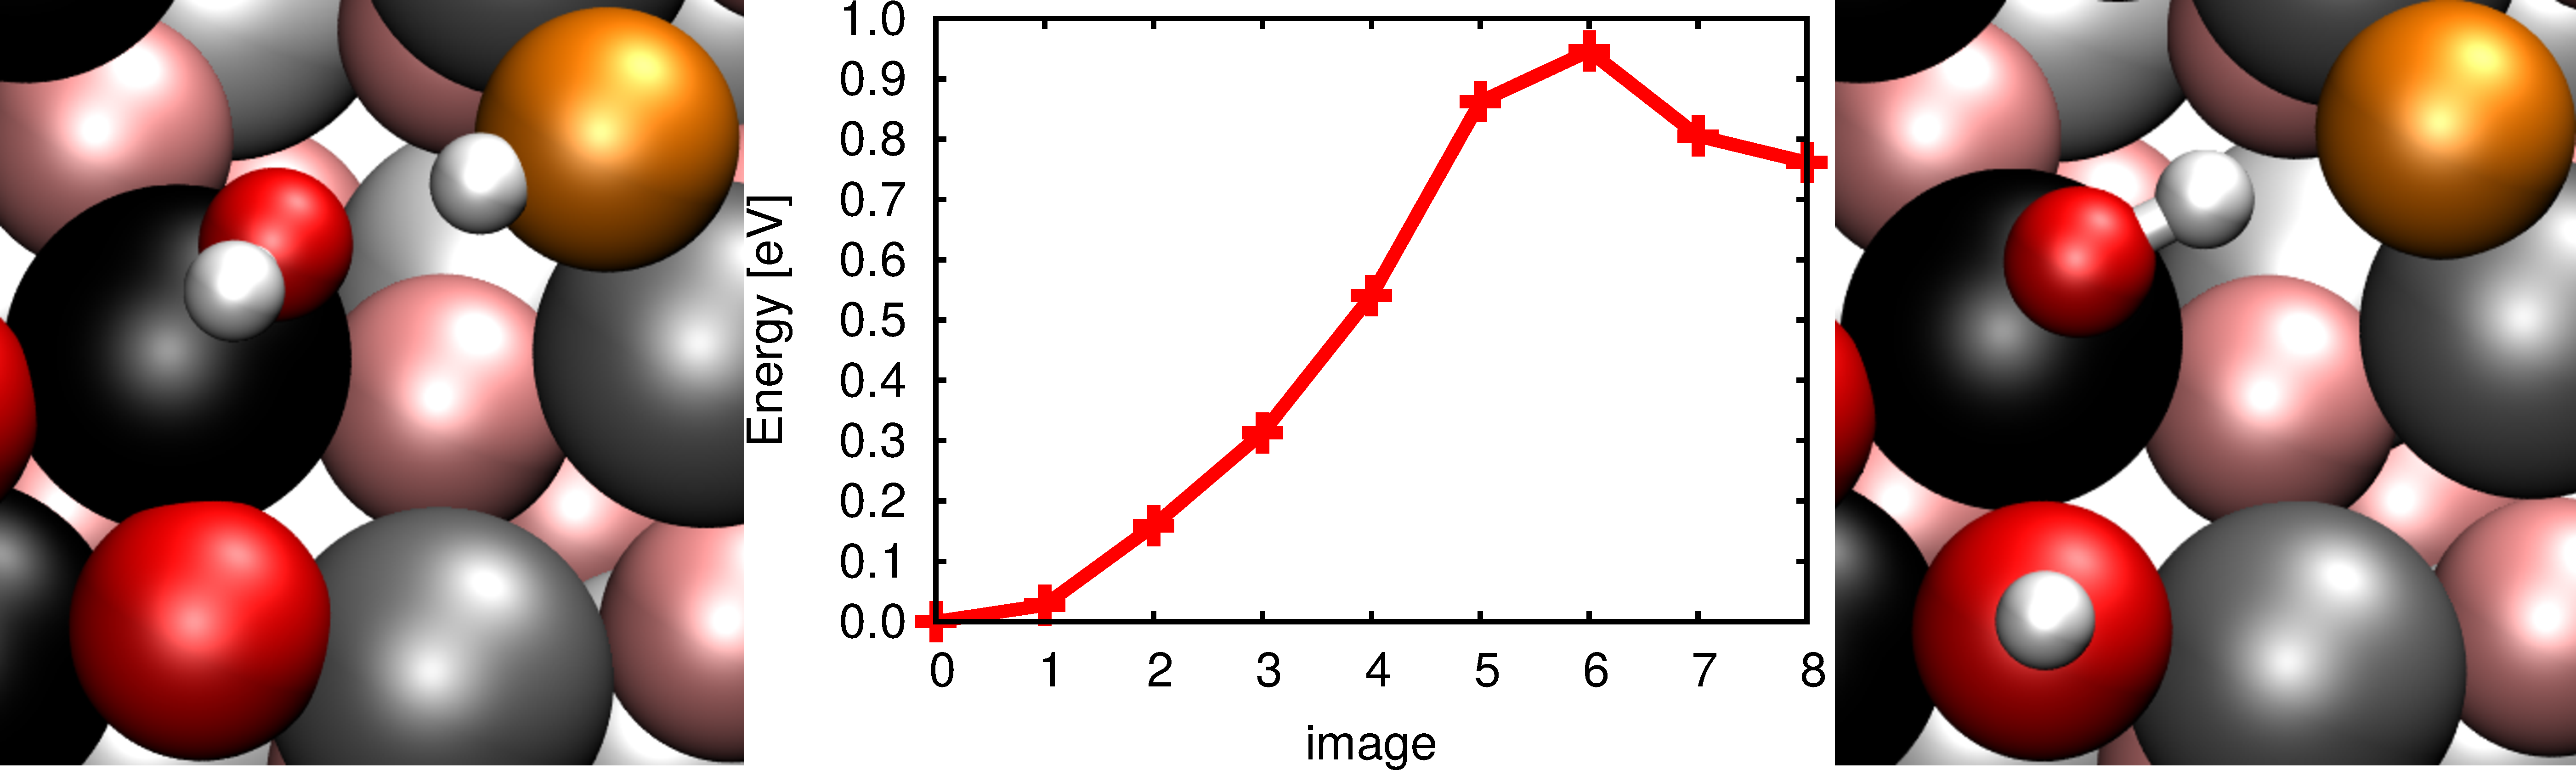
\includegraphics[width=.9\textwidth]{figures/11-20/Diff-H_Cb2-Cb3.pdf}}
\quad
\subfigure[Df-H-b: inter-CUSa$\parallel$O-$\mu_2\rightarrow$inter-CUSa$\parallel$O-$\mu_3^\prime$]{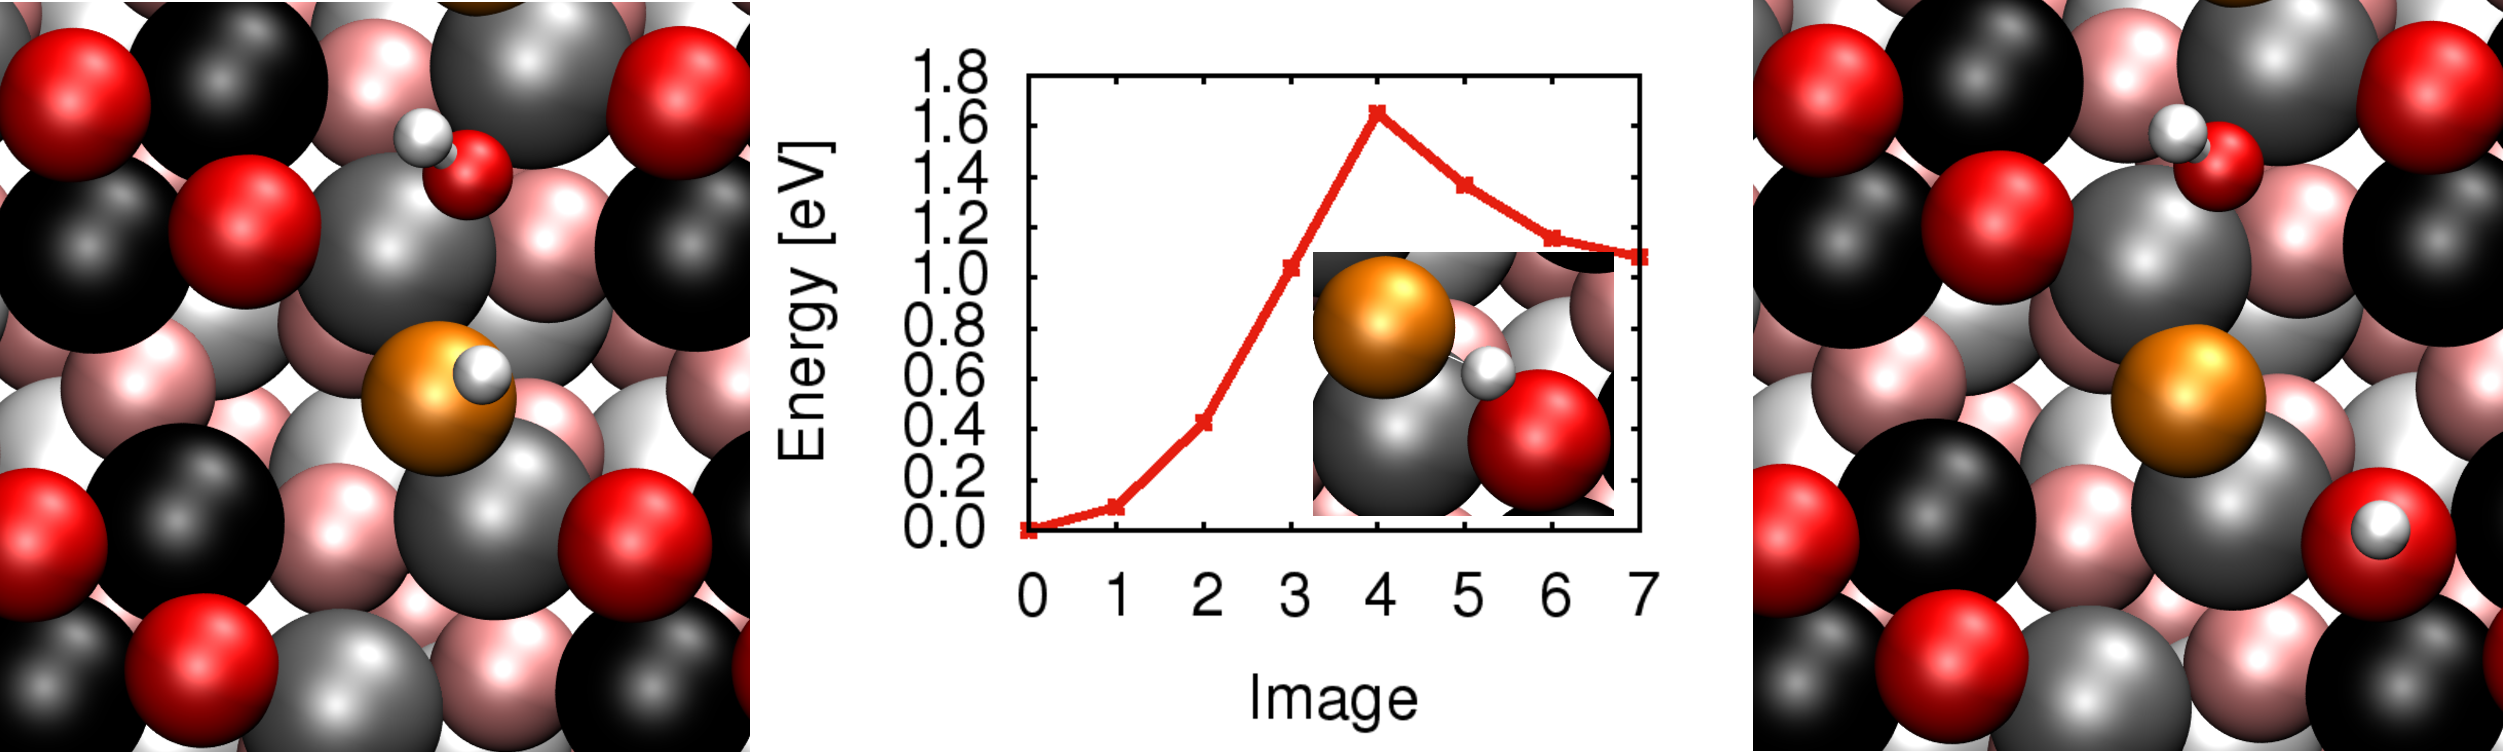
\includegraphics[width=.9\textwidth]{figures/11-20/Diff-H_iCa2-iCa3p.pdf}}
 \quad
 \subfigure[Df-H-c: inter-CUSb$\parallel$O-$\mu_2^\prime\rightarrow$inter-CUSb$\parallel$O-$\mu_3^{\prime\prime}$]{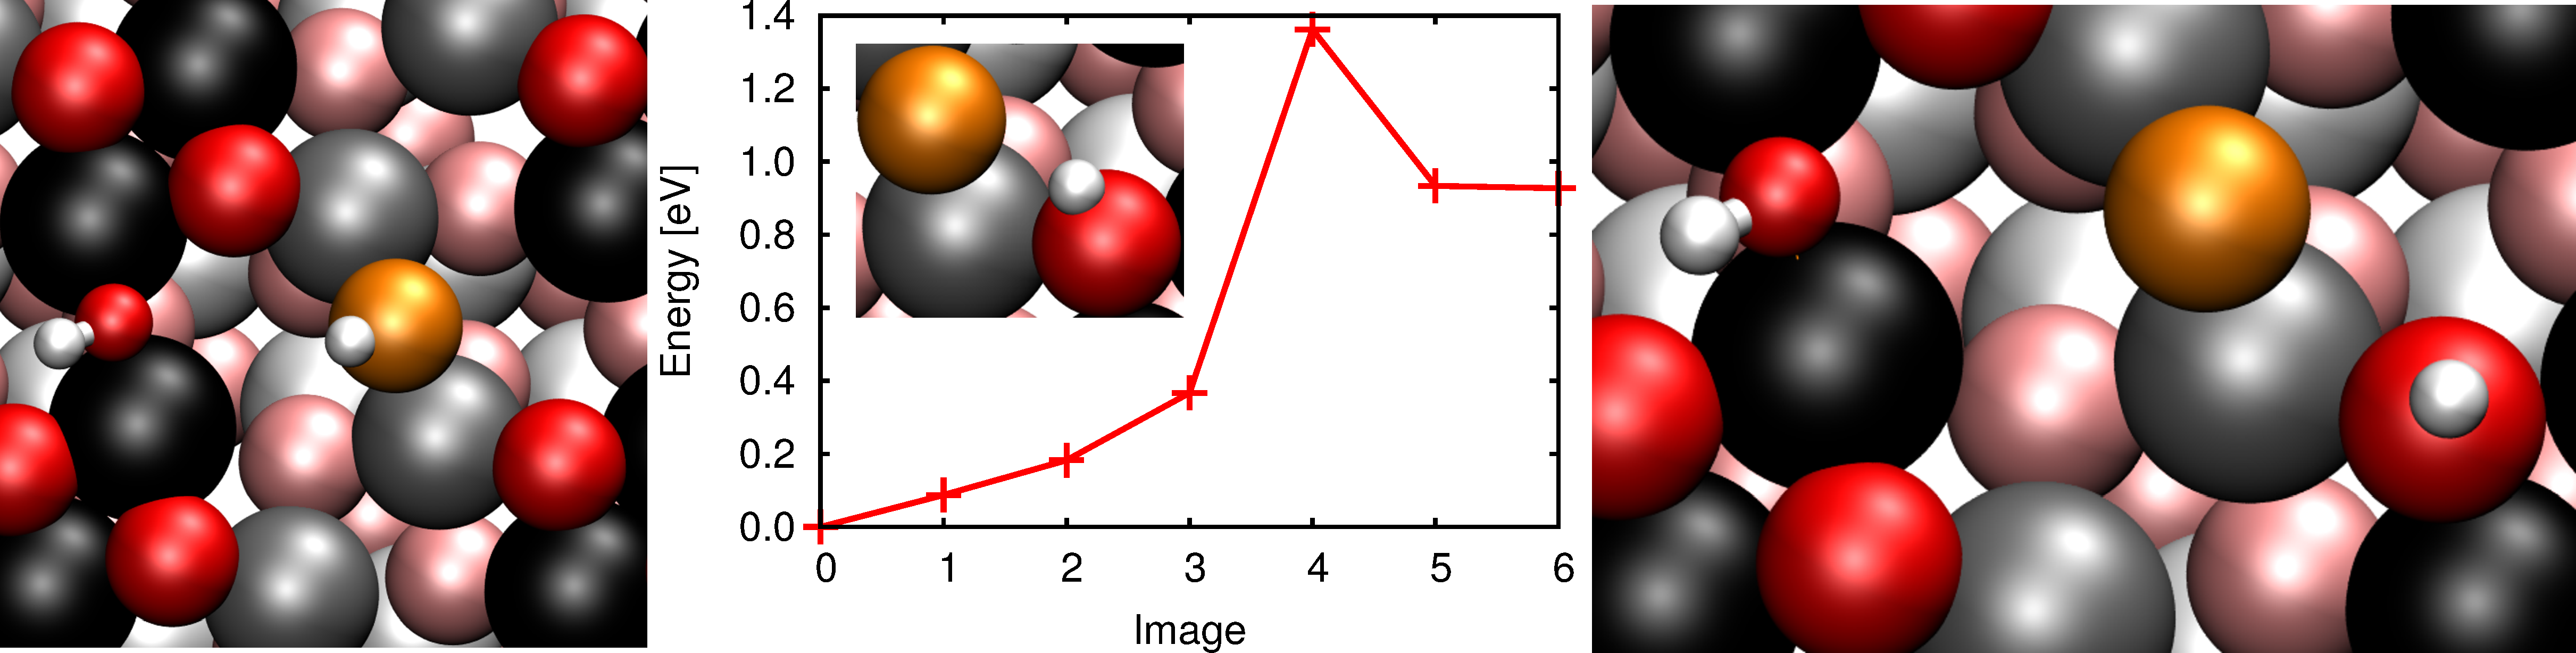
\includegraphics[width=.9\textwidth]{figures/11-20/Diff-H_iCb2p-iCb3pp.pdf}}
 \quad
\subfigure[Df-H-d: inter-CUSb$\parallel$O-$\mu_3^{\prime\prime}$ $\rightarrow$inter-CUSb$\parallel$O-$\mu_3^{\prime\prime\prime}$]{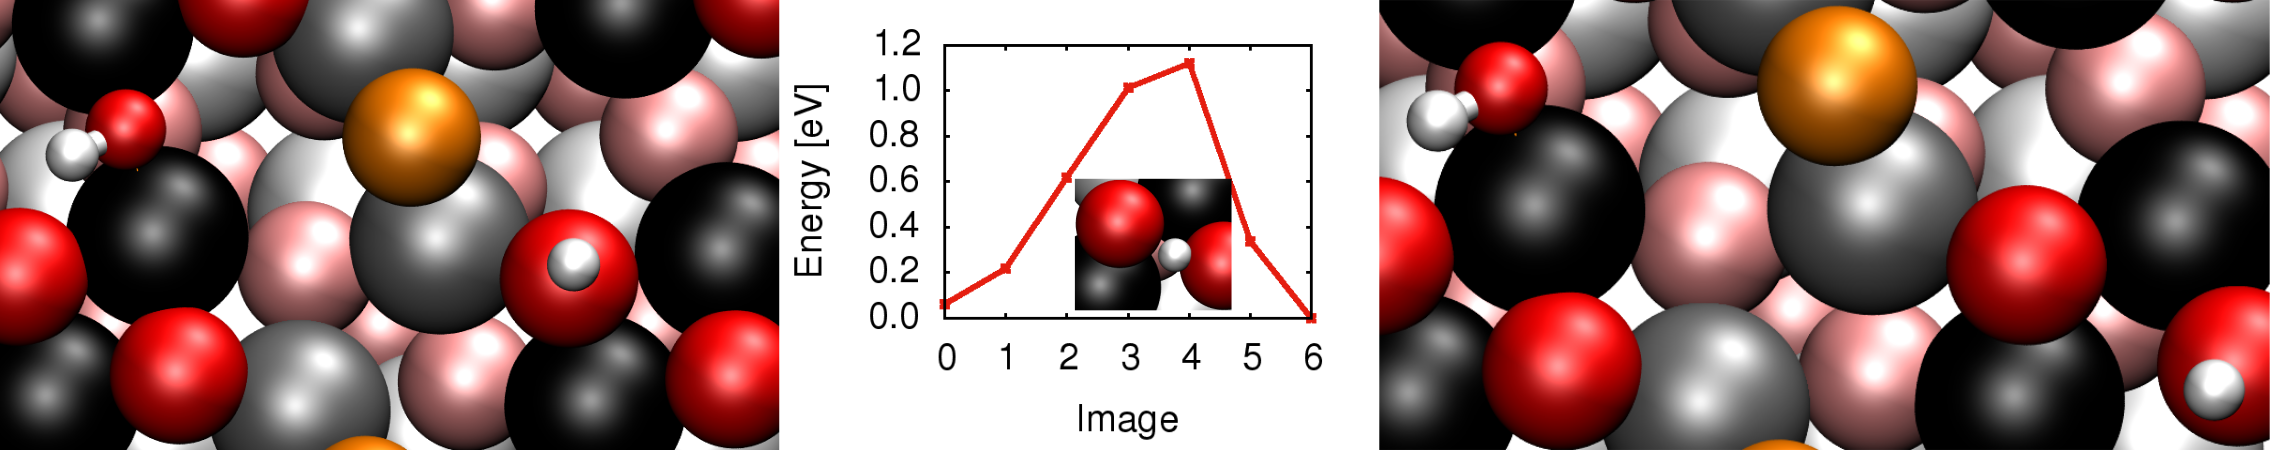
\includegraphics[width=.9\textwidth]{figures/11-20/Diff-H_iCb3pp-iCb3ppp.png}}
\caption{Minimum energy paths with transition states, and both educt and product states for Df-H-a - Df-H-d reactions.
The color code is as explained above.}
       \label{mep2}
\end{figure*}

Rates for backreactions can also be calculated and the results are shown in Table \ref{tab:backreactions}.
\begin{table*}[ht]
  \centering
  \caption{Reaction rate constants for the reactions $\stackrel{\rightarrow}{k}$ (left) in comparison with the backreactions $\stackrel{\leftarrow}{k}$ (right).
These rates can be calculated via detailed balance $\stackrel{\leftarrow}{k}  = \stackrel{\rightarrow}{k} \ e^{-\Delta G/k_B T}$.
All values are given in s$^{-1}$ at a temperature of $300\,$K.}
  \begin{tabular}{cl|cc|cc|c}
  \toprule
\small{Reaction Type} & \small{$\stackrel{\rightarrow}{k}(\textrm{300\,K})$(s$^{-1}$)} &  \small{$\stackrel{\leftarrow}{k}(\textrm{300\,K})$(s$^{-1}$)} \\\midrule
%  &forward reaction &back reaction \\\midrule
 \small{D-a}   & \small{5.76$\times 10^{12}$} &\small{1.17$\times 10^4$}\\
 \small{D-b}   & \small{\textit{3.0$\times$10$^{13}$}} & \small{n.f.} \\
 \small{D-c}   & \small{n.f.} & \small{n.f.}  \\\midrule
 \small{Df-OH-a} & \small{1.88 $\times  10^6$}&\small{9.86$\times 10^9$} \\
 \small{Df-OH-b}  & \small{2.41$\times 10^{-6}$}& \small{1.69$\times 10^{-8}$}\\\midrule
 \small{Df-H-a} & \small{\textit{4.53$\times$10$^{-3}$}} &\small{n.f.} \\
 \small{Df-H-b}  & \small{4.90$\times 10^{-13}$} &\small{1.49$\times 10^5$} \\
 \small{Df-H-c} & \small{9.96$\times 10^{-10}$}& \small{9.95$\times 10^5$}\\
 \small{Df-H-d} & \small{1.05$\times 10^{-3}$} &\small{7.12$\times 10^{-5}$} \\\bottomrule
  \end{tabular}
  \label{tab:backreactions}
\end{table*}
\\\\

As mentioned before an immense and well known problem of GGA is that barriers are underestimated\cite{Zhao05}.
Optimizing structures with the hybrid functional such as HSE06 are infeasible due to high computational cost. %more than a year with 16CPU without convergence.
A further attempt doing HSE06 single point calculations on PBE-optimized transition state was not very accurate and did not deliver better results (unpublished work by Dr. J. Wirth, Universtität Potsdam).
With this, the PBE results may not be perfectly accurate, but these are still the best we can afford with the computational power at the moment.

\clearpage
\section{Vibrational Frequencies}\label{sec:vib11-20}

Vibrational spectroscopy is a great source of knowledge about chemical systems.
The frequencies of vibrations give hints about the chemical environment as hydrogen bonds and other atoms nearby that bind to each other.
These vibrational frequencies were calculated for the surface system adsorbed with OD.
Our experimental partners from FHI use deuterated water (D$_2$O) instead of H$_2$O because the chemical reactivity is the same but the spectroscopic properties are clearer with their applied Laser system, so that all results presented in this particular section are given for D$_2$O.
The experimental Sum Frequency Generation (SFG, a surface specific vibrational spectroscopy) spectra for the OD range of the low coverage regime for two different coverages are shown in Figure \ref{abb:exp-sfg} as they were published in \cite{Heiden11-20_2018}.
\begin{figure}[!ht]
 \centering
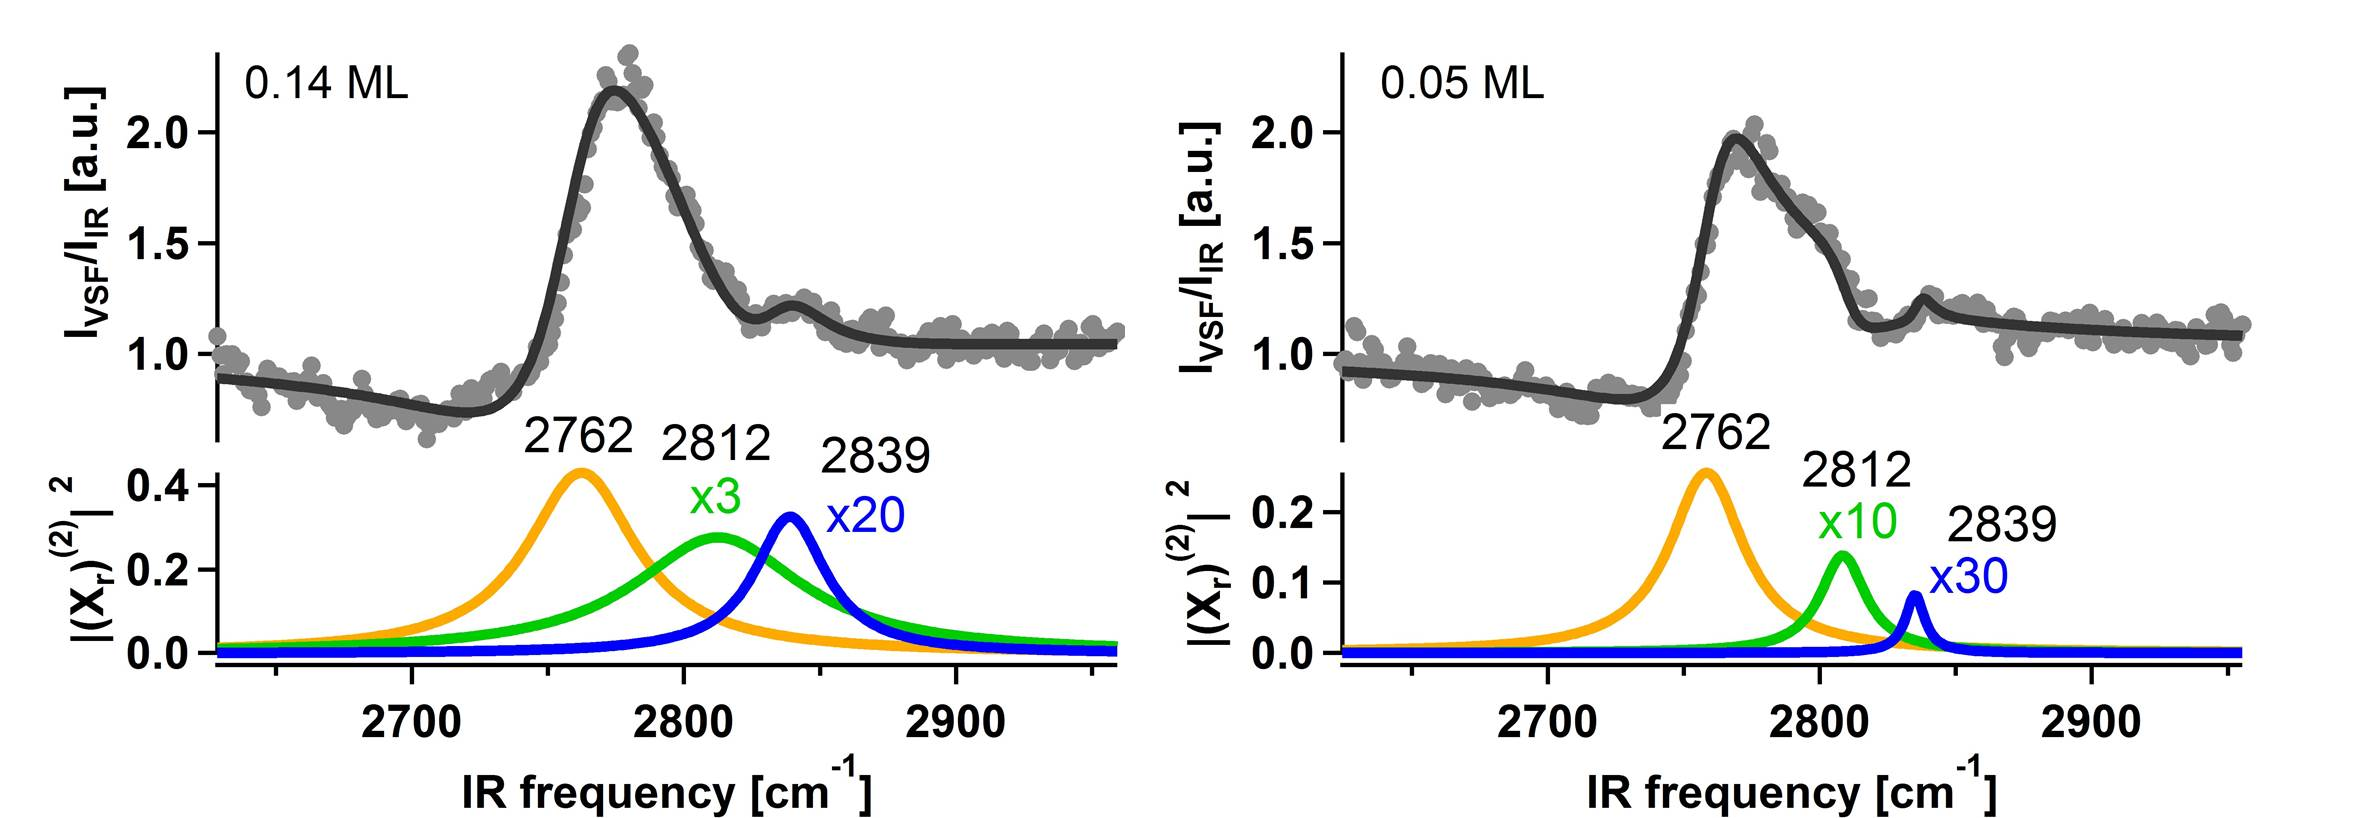
\includegraphics[width=0.9\textwidth]{figures/11-20/SFG_fit.jpg}
 \caption{Experimental SFG results for (11\=20) surface with 0.14ML (mono layer, left spectrum) and 0.05ML water coverage (right) including fit.
The experiment was conducted by Yanhua Yue from the ``Interfacial Molecular Spectroscopy'' group at the Fritz Haber institute (FHI) in Berlin.
Coverage only influences intensity of the peaks but not the peak position itself.
The different coverages are achieved via different preparing temperatures of the sample.}
        \label{abb:exp-sfg}
 \end{figure}
% Of course, the frequencies for a deuterated system are different from OH, but the different isotopes can be calculated easily within vasp, just by changing the mass.


In the experiment the alumina single crystal was cleaned in ethanol and Milli-Q water and dried with N$_2$ before being installed in the ultra high vacuum chamber.
It was then sputtered in Ar, and annealed to high temperatures in ultra high vacuum (UHV, $2.5\times 10^{-10}\,$mbar) and afterwards sputtered three times in oxygen at different temperatures.
After this treatment, D$_2$O was brought onto the surface with a molecular beam source (MBS).
The SFG measurement was then conducted at $130\,$K.
A short overview explaining the basics of experimental methods of interest for this work can be found in Appendix \ref{exp_techniques}.
For further experimental details see \cite{Heiden11-20_2018} and the supporting information therein.
Test with a symmetric slab (where at the top and the bottom water is adsorbed) were computed, discovering that the asymmetric model including dipole corrections is sufficient to describe the system.
Only minor differences could be obtained.
Details for this are given in Appendix \ref{symmetric_slab}.
\\
\\

To calculate the vibrational modes in this work mainly two methods were applied: Normal mode analyses and power spectra from AIMD via the velocity-velocity autocorrelation function.
However, the latter results are not fully converged yet and have to be propagated tens to hundred ps instead of $1$-$2\,$ps, so only preliminary results will be shown to illustrate the power of this method.


The focus is mainly on the peak position rather than their intensities, because in the first place it is of greater importance what kind of vibrations gives which peak than the intensity of the peak itself.
Also, it is still challenging to determine the frequencies in good comparison with experimental findings before heading to intensities.


In the normal mode analyses this work follows two distinct approaches: dipole corrections and Born effective charges.
However, in the power spectra from MD calculations the intensities are not directly retrieved but as said before, we are more interested in the peak position.
\\\\

In subsection \ref{nma}, OD stretch vibrations are presented but also modes for higher coverage systems and lattice vibrations are examined.
% But not only the OD frequencies are of interest, but also the lattice vibrations, and are covered in both subsections.
Subsection \ref{bec} gives the spectra including intensities determined via Born effective charges and in subsection \ref{vvacf} the results from the velocity-velocity autocorrelation function are shown.

\subsection{Normal Mode Analysis}\label{nma}
\subsubsection{OD Vibrations}

The normal modes are calculated within the harmonic approximation and depend on the mass and the spring constant of the bond.
This ansatz is quite good for high frequency modes like OD stretch vibrations.
We assume that the OD stretching modes for the three most stable structures would contribute to the spectrum the most, since the less stable adsorbed species are improbable to appear.
The corresponding wavenumbers are presented in Table \ref{tab:freq_layers} for different slab sizes, as given in Figure \ref{abb:cell_sizes}.
Also the angle of the OD bond with respect to the surface is given (see Table \ref{tab:freq_layers}), since vibrations which are in plane cannot be detected with SFG spectroscopy (sum frequency generation) and hence the intensity is a function of this angle.
\begin{table*}[th]
  \centering
 \caption{Wavenumbers of normal modes for the different slab sizes: OD stretching modes for each of the most stable minima.
All values are given in cm$^{-1}$; in parantheses, the angle of the OD bonding vector to the surface normal ($\theta$ in \textdegree) is provided.
In each column, the left value reflects the adsorbed OD$_\textrm{ads}$ group and the right wavenumber the surface OD$_\textrm{surf}$ group, respectively.
 In the right part a sketch of the angle $\theta$ between the OD bond and the surface normal is shown.}
\vspace*{.2cm} 
 \begin{tabular}{l|ccccc}
 \toprule
  Layers&inter-CUSa$\parallel$O-$\mu_2$ &CUSb$\parallel$O-$\mu_2$  &inter-CUSb$\parallel$O-$\mu_2$&\multirow{6}{1pt}{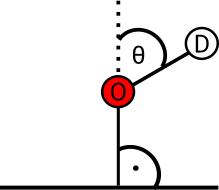
\includegraphics[width=2cm]{figures/11-20/ODangle.png}} \\\midrule
  10 &2731 (44), 2694 (36) &2785 (26), 1711 (61) &2692 (41), 2689 (54)& \\
  15 &2728 (44), 2695 (36) &2783 (24), 1812 (60) &2711 (34), 2656 (60)& \\
  20 &2729 (44), 2694 (35) &2783 (24), 1838 (60) &2715 (34), 2665 (58)& \\
  25 &2728 (44), 2696 (35) &2767 (59), 1750 (62) &2764 (29), 2724 (41)& \\\midrule
  exp. & \multicolumn{3}{c}{2839, 2812, 2762}& \\\bottomrule
  \end{tabular} 
  \label{tab:freq_layers}
\end{table*}
\\\\

 Following this approach we expect six modes to appear: an OD$_\textrm{surf}$ and an OD$_\textrm{ads}$ for each of the three.
In all cases the relationship between the two individual modes for each considered structure is portrayed by $\tilde{\nu}$(OD$_\textrm{ads}$)>$\tilde{\nu}$(OD$_\textrm{surf}$).
This can be explained with the different reduced mass for both vibrations: The OD$_\textrm{surf}$ oscillator has a slightly larger reduced mass since the deuterium is bound directly to the surface, whereas the adsorbed OD group can act more as a quasi-free OD group \cite{Wirth2014}.
All these vibrations are clearly localized on one of the OD groups which suggests that the normal modes ansatz is reasonable.
Of course, normal modes of all molecular and next neighbor dissociated structures from 10 to the 25 slab layer model were calculated, although the slab was already converged with 10 layers concerning OD stretch frequencies as mentioned in section \ref{structure_search11-20} and in Table \ref{tab:freq_layers}. 
\\
\\

To consider the probability of observing the three dissociated species, their respective Boltzmann weights $P_i$ were evaluated:
\begin{equation}\label{boltzmann-weight}
 P_i=e^{-G_i/(k_BT)}
\end{equation}
with the free energy $G_i$ that is obtained from the frequencies of the vibrations.
With this analysis it is possible to show the relative population for different temperatures, given in Table \ref{tab:boltzmann-pop}.
In the temperature range relevant for the experiments, it is shown that the population of the species inter-CUSa$\parallel$O-$\mu_2$ clearly dominates and furthermore that the population of inter-CUSb$\parallel$O-$\mu_2$ is very low compared to the others.
\begin{table*}[th]
  \centering
 \caption{Boltzmann population $P$ relative to the most stable inter-CUSa$\parallel$O-$\mu_2$, calculated according to Equation \ref{boltzmann-weight} for $130$, $300$ and $400\,$K.
Values are given for the 10 layer system.}
\vspace*{.2cm} 
 \begin{tabular}{l|ccc}
 \toprule
  & P$_{130K}$ & P$_{300K}$ & P$_{400K}$\\\midrule
  inter-CUSa$\parallel$O-$\mu_2$ &1 &1 &1 \\
  CUSb$\parallel$O-$\mu_2$ & 1.4$\times 10^{-6}$& 6.1$\times 10^{-3}$& 3.2$\times 10^{-2}$\\
  inter-CUSb$\parallel$O-$\mu_2$ & 1.0$\times 10^{-15}$ & 1.2$\times 10^{-6}$ & 6.6$\times 10^{-5}$\\\bottomrule
  \end{tabular} 
  \label{tab:boltzmann-pop}
\end{table*}


From the results for the frequencies of the three most stable structures (from Table \ref{tab:freq_layers}), one can see four relevant modes to be expected for all slab sizes.
One of them is noticeably lower in energy due to hydrogen bonding (OD$_\textrm{surf}$ vibration of CUSb$\parallel$O-$\mu_2$).
Also the angle of the bonding vector with respect to the surface normal is very high (\textit{i.e.} the bond is more in plane, values and schematic representation shown in Table \ref{tab:freq_layers}) so that the expected intensity is remarkably lower and may be not visible in experiment because of the angle dependence of the intensity in SFG.


With this in mind, we are able to predict three peaks, which fits well to the experimental results of Yanhua Yue from FHI Berlin (see Figure \ref{abb:exp-sfg}).
Similar to existing literature\cite{Wirth2014}, comparing these results in absolute numbers is not very impressive, but relative wavenumbers are in good agreement, see results for experiment and all different sized layer slabs in Table \ref{tab:rel_modes}.
\begin{table*}[!h]
\begin{center}
\caption{Wave number differences $\Delta \tilde{\nu}$ are given in [cm$^{-1}$].
$\Delta \tilde{\nu}_1$ depicts the difference between the surface OD group of the inter-CUSa$\parallel$O-$\mu_2$ species and the respective surface OD group on O-$\mu_2$ and  $\Delta \tilde{\nu}_2$ is the difference between the same surface OD group and the adsorbed OD group on CUSb from CUSb$\parallel$O-$\mu_2$.}
\begin{tabular}{ccc}
\toprule
layers & $\Delta \tilde{\nu}_1$ &  $\Delta \tilde{\nu}_2$\\\midrule
10  &37 &91 \\
15  &33 &88 \\
20  &35 &89 \\
25  &32 &71 \\\midrule
exp.&50 &77 \\\bottomrule
  \end{tabular}
\label{tab:rel_modes}
\end{center}
\end{table*}
It becomes clear that for OD stretching bonds there is no visible trend: The 10 layer system already gives reasonable results and none of the employed larger slab models brings any improvement.
\\
\\

Two problems of this approach are that we neglect anharmonicities, which are especially important for hydrogen-bonded vibrations, and neighbor effects.
The latter can be solved by computing higher coverage systems.



\subsubsection{Complete Spectrum: Intensities from Dipole Corrections}\label{phonons}

The spectra for both the OD range and the lattice range are presented in this subsection.
All spectra shown in this section were normalized to the most intense peak, with the intensities being determined by dipole corrections.
Note, that the intensities in the OD range decrease with growing slab size since they are normalized to the most intense peak in the lattice region.
For smaller slab sizes the ratio between OD and lattice is higher than for bigger slab sizes, so that the OD intensities in direct comparison seems smaller.
This however, has no physical meaning.
In some figures short notations for the adsorbed species are used: iCa2 for inter-CUSa$\parallel$O-$\mu_2$, Cb2 for CUSb$\parallel$O-$\mu_2$ and iCb2 for inter-CUSb$\parallel$O-$\mu_2$.
Unfortunately, experimental results for the spectral range of the lattice vibrations are not obtained by our experimental partners yet, so that no comparison to SFG modes can be made.
% \todo{experimental results are still missing, compare modes of low coverage limit to spectra with higher coverage, ask Lu for more data of higher coverage.}


In the spectra from the dipole corrections ($\Gamma$-point only calculated normal mode analyses with dipole corrections in z direction) the intensities are given by the square of the dipole moment $\mu^2$ to which it is proportional.
That is why in the spectra the y-axis is given as $\mu^2$.
For the lattice vibrations the same normal modes of the ten layer slab were checked to get a first impression about the spectra.
But for a better description of the deeper lying phonon vibrations we need to consider more layers of the bulk in order to get more reliable results.
From an experimental point of view it is suggested that SFG spectra can give insight into at least three atomic layers of the bulk.
To make sure these are described well, the system size was expanded, performing calculations for the most stable adsorption geometries for more layered systems, going up to $6\times 5=30$ atomic layers (with five being the number of atomic layers in the unit cell in z direction, compare Figure \ref{abb:cell_sizes}), for the clean surface and for 25 layers for the adsorbate covered surface.
The differences arise from slightly different modes because more or less atomic layers are taken into account.
These more layered optimized geometries do not differ strongly from the ten layer ones that were presented in Section \ref{structure_search11-20}, Figure \ref{abb:ads-geoms} and hence are not shown.
% \todo{here, maybe Appendix? Not necessary}.
Respective adsorption energies can be found in Table \ref{tab:eads_layers}.
For the low energy modes, one has to keep in mind that normal modes may not be a perfect description of these deeply delocalized vibrations but still might be sufficient.


The results for the clean surface are shown in Figure \ref{abb:clean_comp_layer}.
For different sized slabs, the results differ largely.
Especially the ten layer system is shifted strongly to lower energy compared to the other slab sizes.
From Table \ref{tab:comp_norm-modes_clean} it can be concluded that the most intense peak is shifted to higher wavenumbers with increasing slab size.
Although the OD vibrations are converged for the ten layer system, the lattice vibrations are not sufficiently described by the system that leads to these wavenumber shifts.


For each slab size the peaks of the vibrational modes show the behaviour of the density of states in the Debye model\cite{kittel2002}:
\begin{equation}
 D(\omega)=V\omega^2/(2\pi^2v^3)
\end{equation}
with the unit cell volume $V$ and the speed of sound $v$.
From the frequency one can evaluate the Debye temperature $\theta_D=\hbar c \omega_D/k_B$, which is linear to the Debye frequency $\omega_D$ which is the highest possible frequency for phonon modes.
In Figure \ref{abb:clean_comp_layer} we can see a quadratic growth of the modes' intensity until the Debye temperature is reached.
It gives the temperature at which all states are occupied.
This is for $\upalpha$-alumina $\theta_D=1042\,$K which corresponds to a wavenumber of around $724\,$cm$^{-1}$\cite{Goto1989}.
By considering more layers one gets closer to the bulk system, for which the Debye frequency is expected.
\begin{figure}[!h]
 \centering
 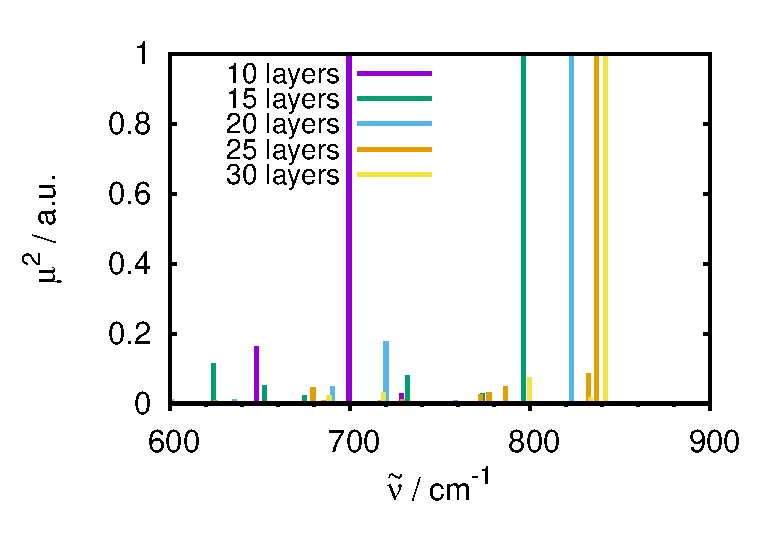
\includegraphics[width=0.8\textwidth]{figures/11-20/comp_freq_surf.eps}
 \caption{Comparison of the spectra for different slab sizes from 10 to 30 layers for the clean surface obtained with normal mode analyses and intensities from dipole corrections.}
 \label{abb:clean_comp_layer}
\end{figure}
\begin{table}[!h]
  \centering
 \caption{Comparison of the results for the different slab sizes with NMA: most intense peak from dipole corrections of the lattice vibrations for the clean surface.}
\vspace*{.2cm} 
  \begin{tabular}{l|ccccc}
  \toprule
Layers& 10&15&20&25&30 \\\midrule
$\tilde{\nu}$ [cm$^{-1}$] &700 &796& 823&837 & 842\\\bottomrule
  \end{tabular}
  \label{tab:comp_norm-modes_clean}
\end{table}
\\

% These results are also shown with intensities calculated from dipole corrected normal mode analyses in Figures \ref{abb:iCa2_size_comp}, \ref{abb:Cb2_size_comp} and \ref{abb:iCb2_size_comp}.
While this trend is true for the clean surface and the lattice region of the covered systems, it does not hold for the OD vibrations regime.
As already mentioned, the OD frequencies seem to be converged for the ten layer slab and both position and intensity show no eminent difference, see Figures \ref{abb:iCa2_size_comp}, \ref{abb:Cb2_size_comp} and \ref{abb:iCb2_size_comp}.
\begin{figure}[!h]
    \centering
    \subfigure[complete spectrum]{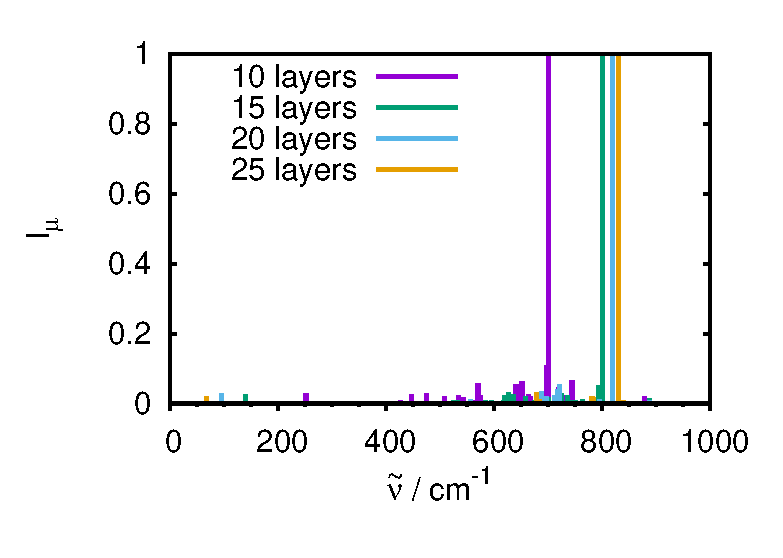
\includegraphics[width=0.45\textwidth]{figures/11-20/comp_freq_iCa2.eps}}
             \quad
             %add desired spacing between images, e. g. ~, \quad, \qquad, \hfill etc. (or a blank line to force the subfigure onto a new line)
    \subfigure[OD stretch regime]{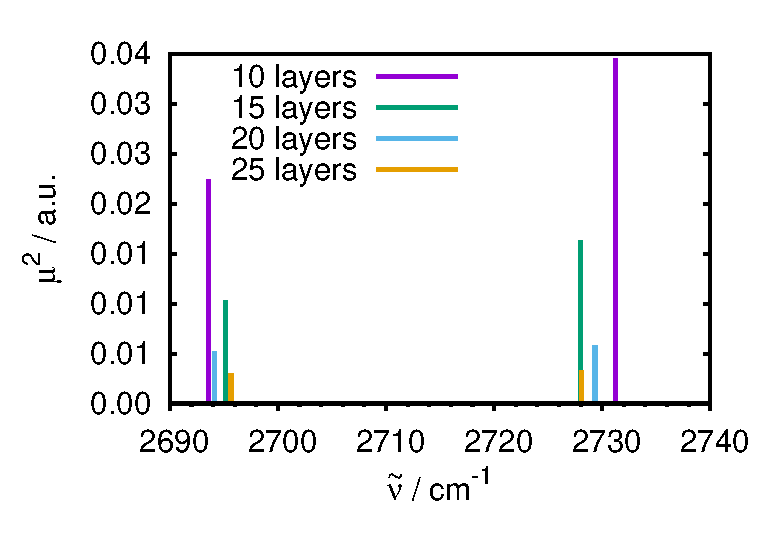
\includegraphics[width=0.45\textwidth]{figures/11-20/comp_freq_iCa2_ODpart.eps}}
             \quad
             %add desired spacing between images, e. g. ~, \quad, \qquad, \hfill etc. (or a blank line to force the subfigure onto a new line)
             \caption{Comparison of inter-CUSa$\parallel$O-$\mu_2$ frequencies for different slab sizes in z direction, obtained by normal mode analyses with intensities from dipole corrections.}
            \label{abb:iCa2_size_comp}
\end{figure}
\begin{figure}[!h]
    \centering
    \subfigure[complete spectrum]{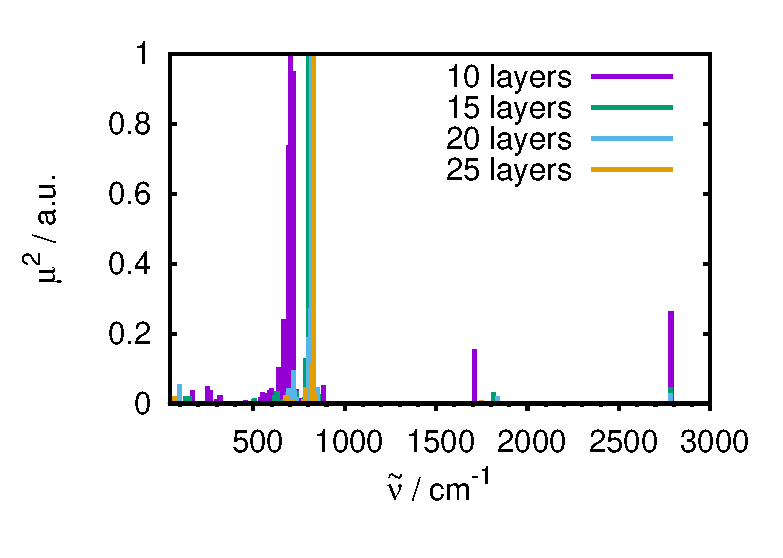
\includegraphics[width=0.45\textwidth]{figures/11-20/comp_freq_Cb2.eps}}
             \quad
             %add desired spacing between images, e. g. ~, \quad, \qquad, \hfill etc. (or a blank line to force the subfigure onto a new line)
    \subfigure[OD stretch regime]{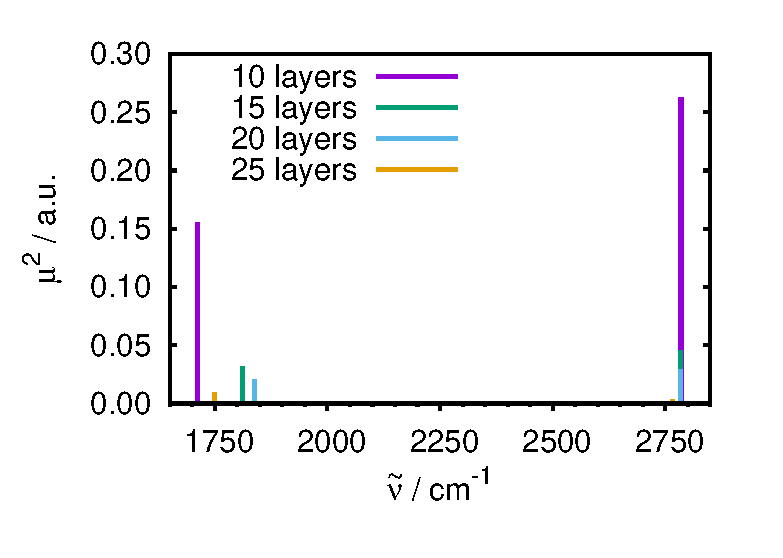
\includegraphics[width=0.45\textwidth]{figures/11-20/comp_freq_Cb2_ODpart.eps}}
             \quad
             %add desired spacing between images, e. g. ~, \quad, \qquad, \hfill etc. (or a blank line to force the subfigure onto a new line)
             \caption{Comparison of CUSb$\parallel$O-$\mu_2$ frequencies for different slab sizes, obtained by normal mode analyses with intensities from dipole corrections.}
            \label{abb:Cb2_size_comp}
\end{figure}
\begin{figure}[!h]
    \centering
    \subfigure[complete spectrum]{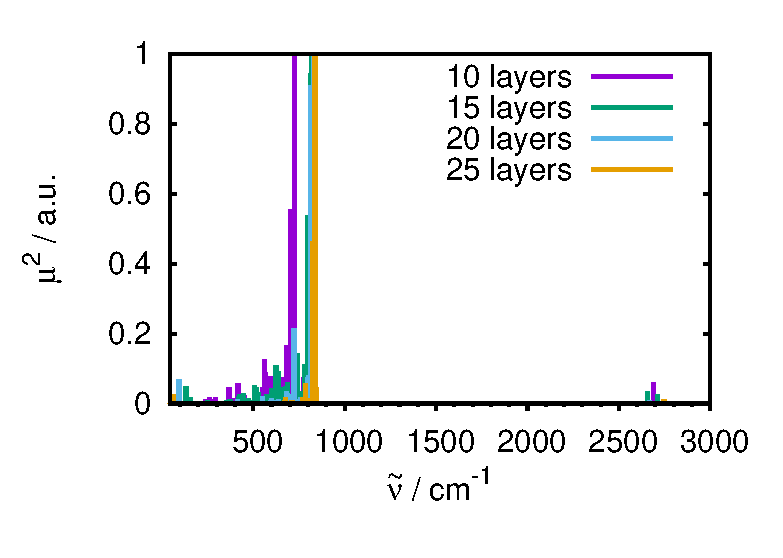
\includegraphics[width=0.45\textwidth]{figures/11-20/comp_freq_iCb2.eps}}
             \quad
             %add desired spacing between images, e. g. ~, \quad, \qquad, \hfill etc. (or a blank line to force the subfigure onto a new line)
    \subfigure[OD stretch regime]{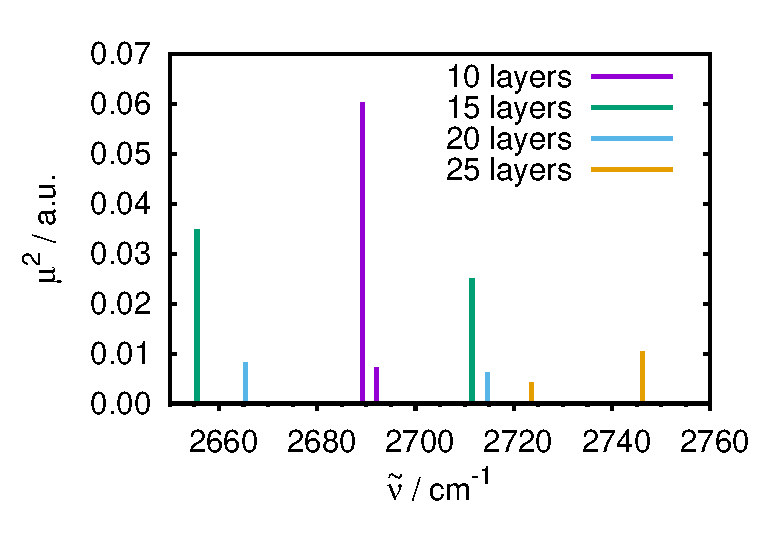
\includegraphics[width=0.45\textwidth]{figures/11-20/comp_freq_iCb2_ODpart.eps}}
             \quad
             %add desired spacing between images, e. g. ~, \quad, \qquad, \hfill etc. (or a blank line to force the subfigure onto a new line)
             \caption{Comparison of inter-CUSb$\parallel$O-$\mu_2$ frequencies for different slab sizes in z direction, obtained by normal mode analyses with intensities from dipole corrections.}
            \label{abb:iCb2_size_comp}
\end{figure}
% In the full spectrum, one can see three different regimes: the lattice region $<900\,$cm$^{-1}$, the OD region around $1700\,$cm$^{-1}$ for hydrogen-bonded stretch and above $2600\,$cm$^{-1}$ for free vibrations.
The exact wavenumbers differ slightly for the OD regions but in general are in good agreement, except for the hydrogen-bonded peak in the CUSb$\parallel$O-$\mu_2$, confer Figure \ref{tab:freq_layers}.
However, the lattice region below $1000\,$cm$^{-1}$ is systematically affected, as in the clean surface system.
Also in the lattice region the quadratic slope of the Debye model can be seen in a textbook like manner.
% \todo{which one fits the experimental results best? wait for experimental results}


The influence of higher coverage was examined for systems already presented in section \ref{structure_search11-20}.
The coverage differs from 2D$_2$O molecules per supercell to four and twelve water molecules, which equals 1ML.
Here the frequencies of the OD stretching modes are affected due to the neighbor adsorbates, for some structures more and for others less (\textit{e.g.} the system with two inter-CUSa$\parallel$O-$\mu_2$).
The higher coverage systems (for structures see Figures \ref{abb:2water}-\ref{abb:4+fully}) were examined.
The total spectrum and the OD range of the 2D$_2$O systems are shown in Figure %\ref{abb:2waterspec}
\ref{abb:2water_comp}, including a comparison between the systems with two D$_2$O molecules and the corresponding systems with only one adsorbate.
% \begin{figure}[!h]
%     \centering
%     \subfigure[spectrum full range]{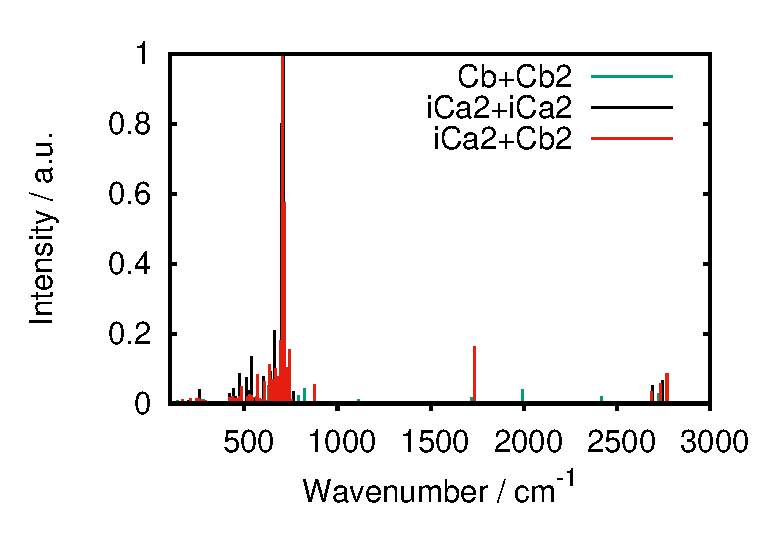
\includegraphics[width=0.45\textwidth]{figures/11-20/specs_dip_2D2O.eps}}
%              \quad
%              %add desired spacing between images, e. g. ~, \quad, \qquad, \hfill etc. (or a blank line to force the subfigure onto a new line)
%     \subfigure[OD range]{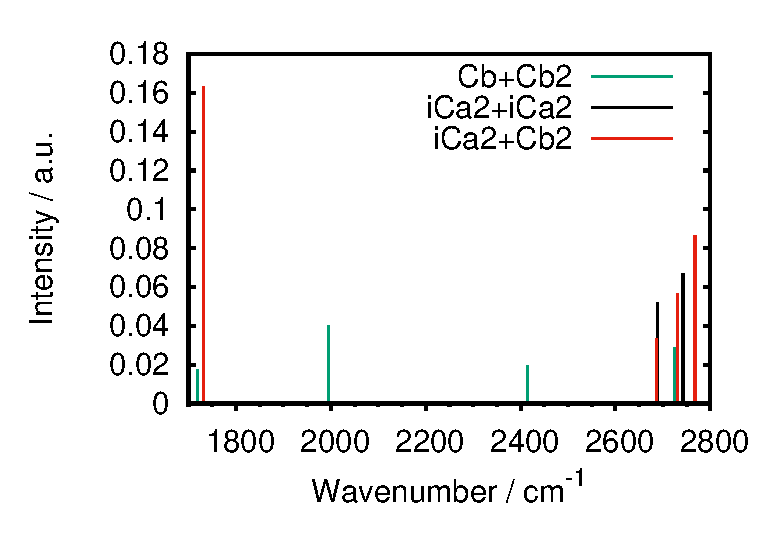
\includegraphics[width=0.45\textwidth]{figures/11-20/specs_dip_2D2O_OD.eps}}
%              \quad
%              %add desired spacing between images, e. g. ~, \quad, \qquad, \hfill etc. (or a blank line to force the subfigure onto a new line)
%              \caption{Spectra from normal mode analyses and dipole intensities for two water molecules per supercell (10 layers).
%(a) shows the full spectral range and (b) only the OD range above $1700\,$cm$^{-1}$.
%The short notations stand for Cb=CUSb, Cb2=CUSb$\parallel$O-$\mu_2$ and iCa2=inter-CUSa$\parallel$O-$\mu_2$.}
%             \label{abb:2waterspec}
% \end{figure}
\begin{figure}[!h]
    \centering
\subfigure[inter-CUSa$\parallel$O-$\mu_2$+CUSb$\parallel$O-$\mu_2$]{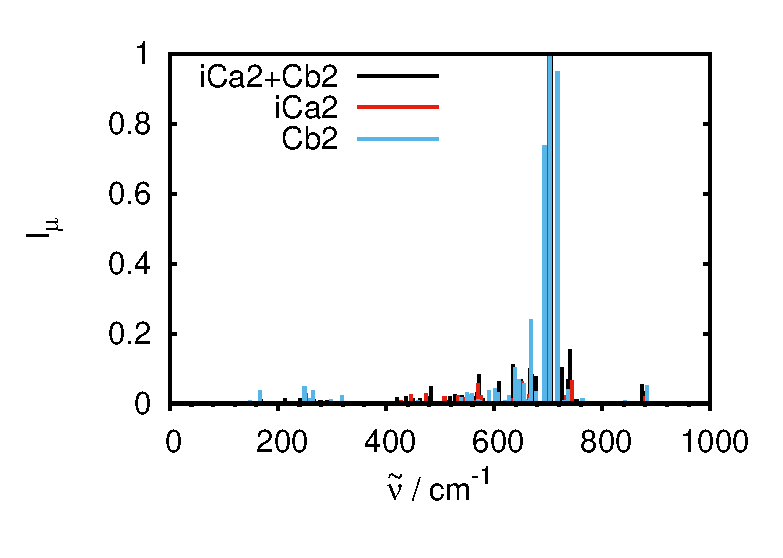
\includegraphics[width=0.45\textwidth]{figures/11-20/comp_iCa2+Cb2.eps}}
            \quad
\subfigure[inter-CUSa$\parallel$O-$\mu_2$+CUSb$\parallel$O-$\mu_2$: OD]{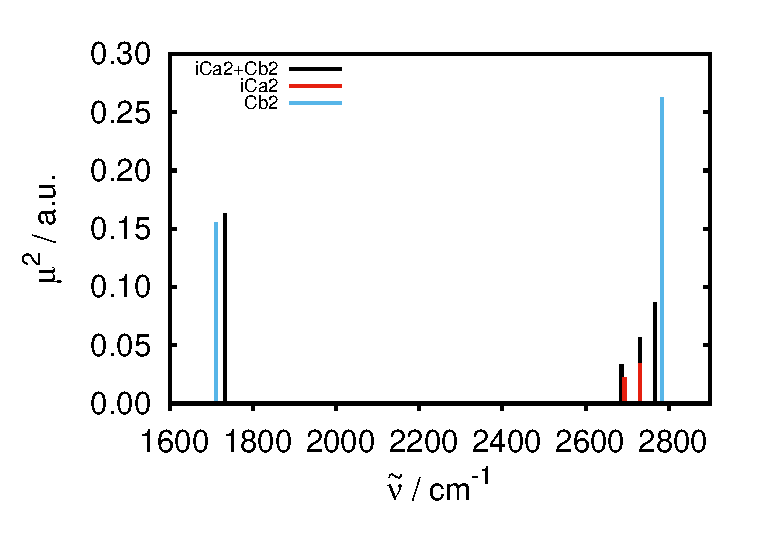
\includegraphics[width=0.45\textwidth]{figures/11-20/comp_iCa2+Cb2_OD.eps}}
\quad
\subfigure[inter-CUSa$\parallel$O-$\mu_2$+inter-CUSa$\parallel$O-$\mu_2$]{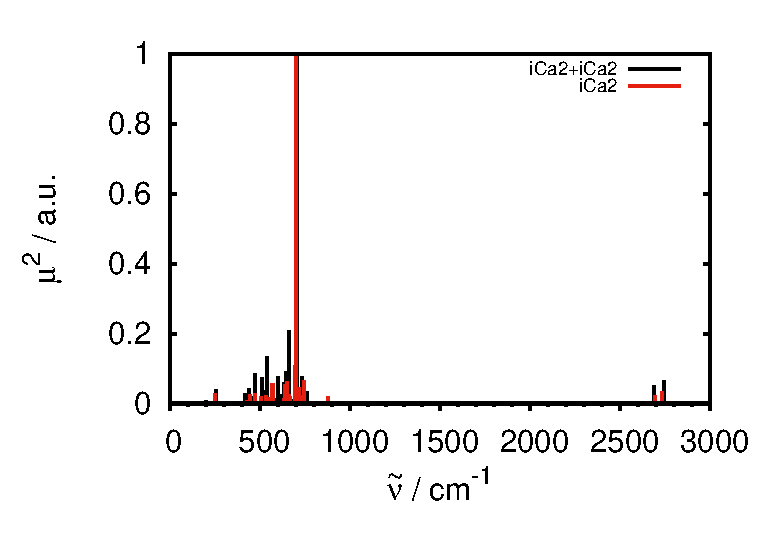
\includegraphics[width=0.45\textwidth]{figures/11-20/comp_iCa2+iCa2.eps}}
             \quad
\subfigure[inter-CUSa$\parallel$O-$\mu_2$+inter-CUSa$\parallel$O-$\mu_2$: OD]{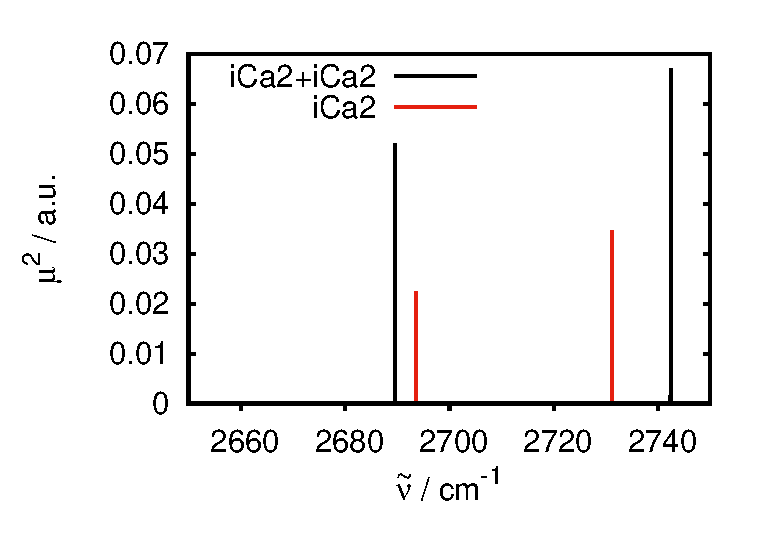
\includegraphics[width=0.45\textwidth]{figures/11-20/comp_iCa2+iCa2_OD.eps}}
\quad
\subfigure[CUSb+CUSb$\parallel$O-$\mu_2$]{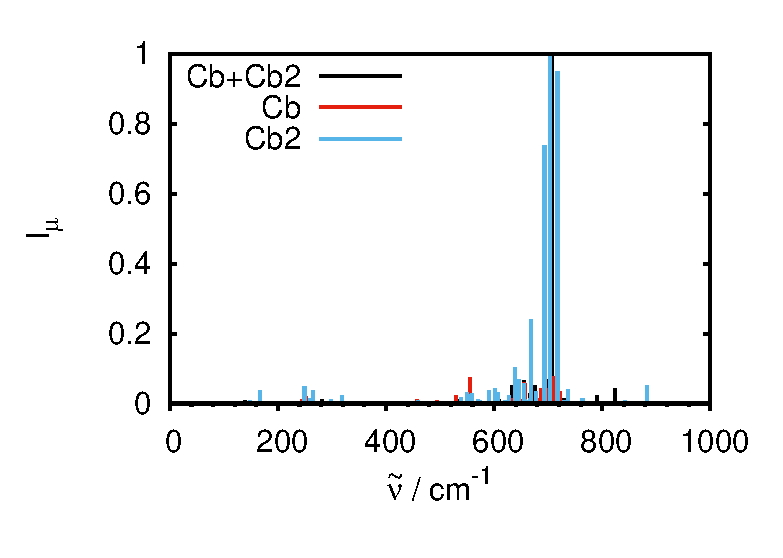
\includegraphics[width=0.45\textwidth]{figures/11-20/comp_Cb+Cb2.eps}}
             \quad
\subfigure[CUSb+CUSb$\parallel$O-$\mu_2$: OD]{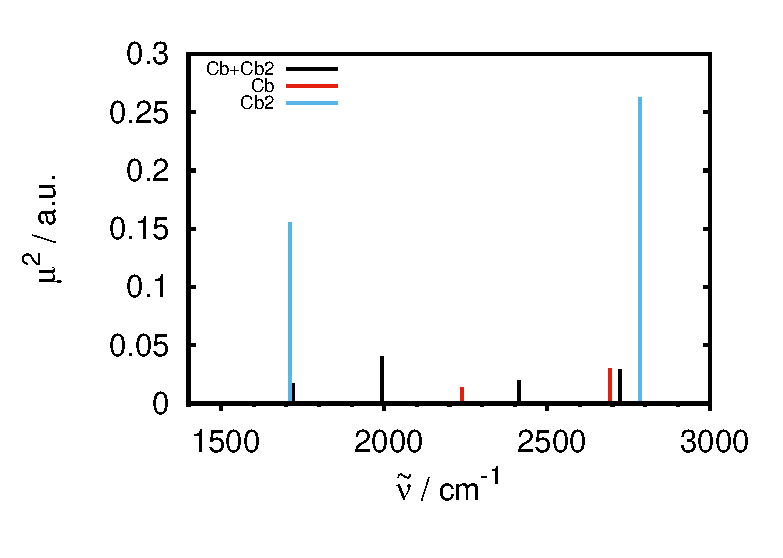
\includegraphics[width=0.45\textwidth]{figures/11-20/comp_Cb+Cb2_OD.eps}}
\caption{Peaks from normal mode analyses and dipole intensities for two water molecules per supercell (10 layers) in comparison with the corresponding systems with one water molecule.
The left row shows the complete spectrum and the right row the OD range.
The abbreviations given are iCa2 for inter-CUSa$\parallel$O-$\mu_2$, Cb2 for CUSb$\parallel$O-$\mu_2$ and iCb2 for inter-CUSb$\parallel$O-$\mu_2$}
            \label{abb:2water_comp}
\end{figure}
For all three systems the agreement between the different slab sizes is reasonably good.
If the water molecules interact strongly with each other, the peaks are shifted heavily.
The system inter-CUSa$\parallel$O-$\mu_2$+CUSb$\parallel$O-$\mu_2$ ((a) and (b) of Figure \ref{abb:2water_comp}) seems to be affected only weakly, inter-CUSa$\parallel$O-$\mu_2$+inter-CUSa$\parallel$O-$\mu_2$ ((c) and (d)) is shifted slightly more.
The system CUSb+CUSb$\parallel$O-$\mu_2$ ((e) and (f)) however, is shifted  significantly, displaying a strong interaction between the molecularly adsorbed and the dissociated groups, stabilizing each other.
This is interesting since in the adsorption energy the three systems acted differently, although there should not be a correlation between the vibrational frequency and the adsorption energy.
The inter-CUSa$\parallel$O-$\mu_2$+inter-CUSa$\parallel$O-$\mu_2$ decreased its stability, whereas the system inter-CUSa$\parallel$O-$\mu_2$+CUSb$\parallel$O-$\mu_2$ did not change and CUSb+CUSb$\parallel$O-$\mu_2$ even was more stabilized.
With this in mind, it makes sense that this system, in which the adsorption energy is slightly affected also shows hardly any difference to the single adsorption in the spectrum.
On the other hand, the system where the molecular water is stabilized by its dissociated neighbor, the spectrum is shifted strongly.
The inter-CUSa$\parallel$O-$\mu_2$+inter-CUSa$\parallel$O-$\mu_2$ is more balanced, because the geometry does not change largely and only the adsorption energy is affected (in a destabilizing way).


Looking at the spectrum of the system with four adsorbed water molecules (1/3 coverage) we obtain Figure \ref{abb:4water}.
\begin{figure}[!h]
    \centering
    \subfigure[spectrum full range]{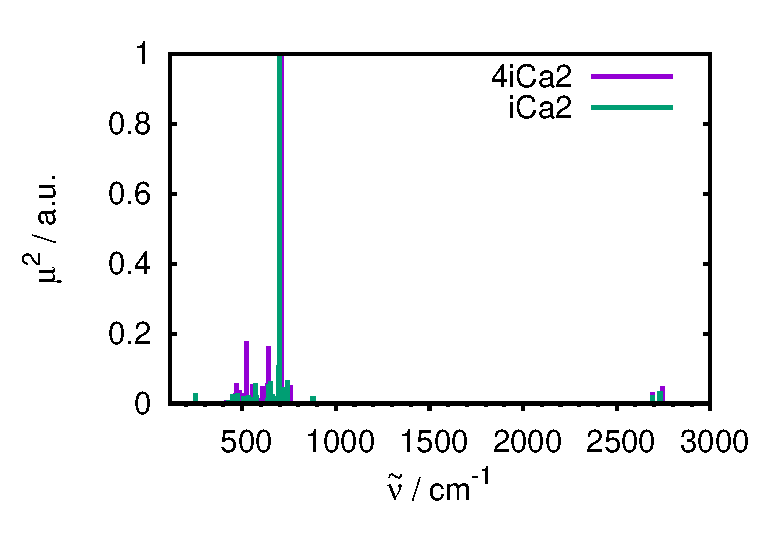
\includegraphics[width=0.45\textwidth]{figures/11-20/spectrum_4iCa2_D2O_2_comp.eps}}
             \quad
             %add desired spacing between images, e. g. ~, \quad, \qquad, \hfill etc. (or a blank line to force the subfigure onto a new line)
    \subfigure[OD range]{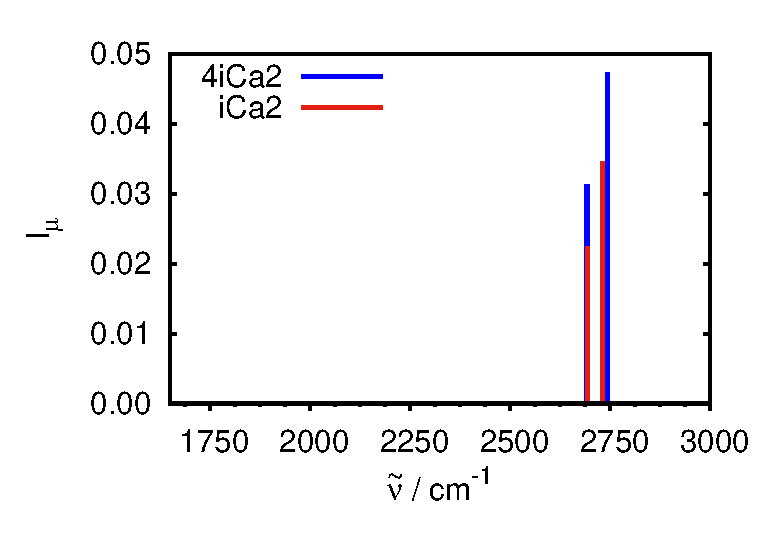
\includegraphics[width=0.45\textwidth]{figures/11-20/spectrum_4iCa2_D2O_2_ODrange_comp.eps}}
             \quad
             %add desired spacing between images, e. g. ~, \quad, \qquad, \hfill etc. (or a blank line to force the subfigure onto a new line)
             \caption{Peaks from normal mode analyses and dipole intensities for four water molecules per supercell (ten layers).
(a) shows the full spectral range and (b) only the OD range above $2680\,$cm$^{-1}$.
The short notations stands for iCa2=inter-CUSa$\parallel$O-$\mu_2$.}
            \label{abb:4water}
\end{figure}
All of these water molecules are adsorbed in inter-CUSa$\parallel$O-$\mu_2$, see Figure \ref{abb:4+fully}(a) and \ref{abb:4water}, which is the most stable and hence the most probable adsorbed species.
As expected, we see the stretch vibrations of the adsorbed residue at higher wavenumbers.
There are three modes for asymmetric (OD oscillators in contrary phases) and one for symmetric stretch vibrations (all OD oscillators in phase) around $2740\,$cm$^{-1}$.
At lower wavenumbers (between $2691$ and $2693\,$cm$^{-1}$) there are localized OD$_\textrm{surf}$ vibrations.
Below that there are delocalized combined vibrations of lattice and OD.
In comparison to the singly adsorbed system (red line) there is an astonishing agreement, both in the OD range and the lattice region.
When looking at the intensities in Figure \ref{abb:4water}(b) one can see that the intensities of the singly adsorbed inter-CUSa$\parallel$O-$\mu_2$ are almost as high as for the system with four dissociatively adsorbed water molecules (and not approximately 1/4 of it).
In contrast to that for the system with two inter-CUSa$\parallel$O-$\mu_2$ species the intensities of the repective mono adsorbed species is halved (see Figure \ref{abb:2water_comp}).
This is probably an artefact of the normalization to the highest peak in the lattice region.


In contrast to the latter systems, for the 1ML system it is not easy to compare to the singly adsorbed species, since it consists of a complex mixture of twelve adsorbed OD residues (on CUSb, inter-CUSa and inter-CUSb), as well as twelve surface OD groups on O-$\mu_2$ but also the less favorable threefold coordinated O-$\mu_3$.
Due to this magnitude of different species, the system possesses many peaks in the OD region, see Figure \ref{abb:fullyhydrox_spec}.
Hydrogen bonding and interaction between groups shift many of the peaks.
Below $900\,$cm$^{-1}$ delocalized OD and lattice vibrations can be found (panel (a)).
In the region between $872$ and $1117\,$cm$^{-1}$ (shown in (b) of Figure \ref{abb:fullyhydrox_spec}) there are bending like vibrations of mostly O-$\mu_2$D groups.
From $\approx2000$ to $2740\,$cm$^{-1}$ various OD stretch vibrations occur.
These are split into three distinct regions: From $\approx 2000$-$2220\,$cm$^{-1}$ in plane vibrations of strongly hydrogen-bonded species can be found.
From $2400$-$2450\,$cm$^{-1}$ in plane vibrations of non hydrogen-bonded species occur and above $2550\,$cm$^{-1}$ out of plane OD stretching bonds appear.
 \begin{figure} [!h]
 \centering
 \subfigure[1ML, lattice range]{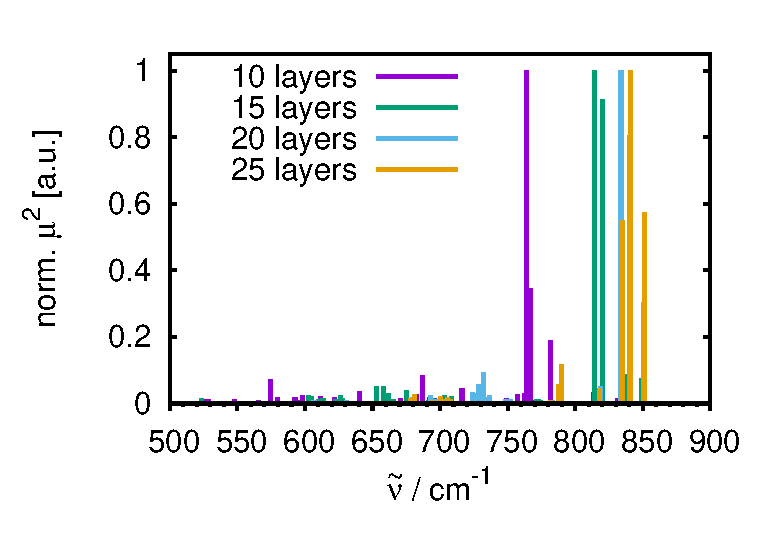
\includegraphics[width=0.45\textwidth]{figures/11-20/fully_cov_D2O_slab-sizes-comp_lattice.eps}}
              \quad
             %add desired spacing between images, e. g. ~, \quad, \qquad, \hfill etc. (or a blank line to force the subfigure onto a new line)
  \subfigure[1ML, low OD range]{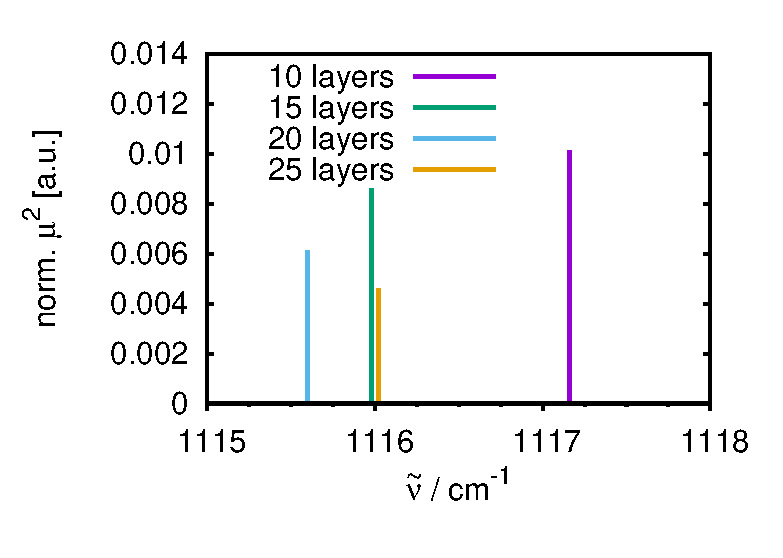
\includegraphics[width=0.45\textwidth]{figures/11-20/fully_cov_D2O_slab-sizes-comp_OD-low.eps}}
              \quad
             %add desired spacing between images, e. g. ~, \quad, \qquad, \hfill etc. (or a blank line to force the subfigure onto a new line)
  \subfigure[1ML, high OD range]{\includegraphics[width=0.45\textwidth]{figures/11-20/fully_cov_D2O_slab-sizes-comp_OD.eps}}%1ML.png}}
 \caption{Comparison of the spectra of the fully with D$_2$O covered surface.
Shown is a comparison between the different slab sizes for (a) the lattice region, (b) the low energy OD range with butterfly like vibrations and (c) the high energy OD range.
The omitted regions do not contain peaks.} 
        \label{abb:fullyhydrox_spec}
\end{figure}
As before, the agreement between different sized slab models in the OD range (without hydrogen bonding) is very good (Figure \ref{abb:fullyhydrox_spec}(c)), in the hydrogen-bonded region around $1116\,$cm$^{-1}$ is convincing (Figure \ref{abb:fullyhydrox_spec}(b)) and only in the lattice region (Figure \ref{abb:fullyhydrox_spec}(a)) is slightly different with the highest energy peak shifted to higher energy with increasing slab size, which is the same trend as for the clean surface and the low coverage systems, which fits the Debye model.
\\\\

Apart from the most stable surface termination (called O-I in \cite{kuri10}), calculations of the second most stable surface termination (O-II), where the uppermost O layer is ``missing'', were performed.
Frequencies were analyzed of the clean surface and the fully covered system, for both the 10 and 25 layer systems.
\begin{figure}[!h]
 \centering
 \subfigure[clean surface]{\includegraphics[width=0.45\textwidth]{figures/11-20/spectrum_O-I-II_comparison.eps}}
 \quad
 \subfigure[fully covered surface]{\includegraphics[width=0.45\textwidth]{figures/11-20/spectrum_O-I-II_fully_comparison.eps}}
 \quad
  \subfigure[fully covered surface, OD range]{\includegraphics[width=0.45\textwidth]{figures/11-20/spectrum_O-I-II_fully_OD_comparison.eps}}
 \caption{Comparison of the 10 layer slab spectra calculated with normal mode analysis and intensities from the dipole corrections.
The clean surface (a), O-I termination (most stable under the whole range of chemical potential) and O-II termination (see Kurita\cite{kuri10}, also relatively stable over a wide chemical potential range).
The comparison of the fully covered O-I and O-II terminations is shown in (b) with a detailed view of the OD range in (c).}
 \label{abb:comp_O-I-O-II}
\end{figure}
In Figure \ref{abb:comp_O-I-O-II} the intensities from dipole corrections for the clean (a) and the fully covered surface termination O-II ((b), (c)) in comparison to the more stable O-I termination are given for the 10 layer slab.
For the clean surface, the spectra deviate by shifted peaks around $50\,$cm$^{-1}$ and different intensity distributions.
In contrast, the differences for the fully covered surfaces are more pronounced due to the different structures including especially more molecularly adsorbed water for the O-II termination.


Also for a larger slab with 25 layers, this comparison was made, see Figure \ref{abb:comp_O-I-O-II_25}
\begin{figure}[!h]
 \centering
 \subfigure[clean surface]{\includegraphics[width=0.45\textwidth]{figures/11-20/comp_O-I_O-II-25.eps}}
%  \quad
%  \subfigure[fully covered surface]{\includegraphics[width=0.45\textwidth]{figures/11-20/spectrum_O-I-II_fully_comparison.eps}}
%  \quad
%   \subfigure[fully covered surface, OD range]{\includegraphics[width=0.45\textwidth]{figures/11-20/spectrum_O-I-II_fully_OD_comparison.eps}}
 \caption{Comparing the O-I and O-II terminated clean surface of the 25 layer system shows very similar results for both systems are obtained.
The most intense peak is shifted by around $20\,$cm$^{-1}$
The growth of the intensities is also quadratic like in the Debye model.}
%Comparison of the 10 layer slab spectra calculated with normal mode analysis and intensities from the dipole corrections.
%The clean surface (a), O-I termination (most stable under the whole range of chemical potential) and O-II termination (see Kurita\cite{kuri10}, also relatively stable over a wide chemical potential range).
%The comparison of the fully covered O-I and O-II terminations is shown in (b) with a detailed view of the OD range in (c).}
 \label{abb:comp_O-I-O-II_25}
\end{figure}
They are very similar and the most intense peak is only shifted by $20\,$cm$^{-1}$.
For the O-I termination the intensities are weaker than for the O-II terminated surface for most vibrations, but overall the differences are not so pronounced.
In the larger slab model there are many more bulk atoms than surface atoms which can contribute to vibrations.
Due to this the differences between O-I and O-II termination get less significant for the larger system.
%\todo{continue here when the calculations are ready! Compare O-I and O-II for 10 and 25 layer slabs, for fully covered.}

\subsection{Complete Spectrum: Intensities from Born Effective Charges}\label{bec}
As a second method to obtain vibrational intensities, Born effective charges were evaluated.
These results were calculated for the three most stable adsorbed systems with ten layers.
For getting the spectrum an angle of the IR beam of 45\textdegree~was assumed.
This choice of this angle weighs the elements of the Born effective charge vector in Equation (\ref{eq:bec}) that are in the sum of the intensity.
Since both the dipole corrections intensities and the BEC calculations are based on normal modes, the frequencies are equal and only the intensities can differ.
In Figure \ref{abb:bec} the spectra for the three most stable structures can be seen, (a) depicts the whole range and (b) the OD range only.
\begin{figure}[!h]
    \centering
    \subfigure[BEC, D$_2$O]{\includegraphics[width=0.45\textwidth]{figures/11-20/bec_specs_dip_D2O_sticks.eps}}
             \quad
    \subfigure[BEC, D$_2$O, OD range]{\includegraphics[width=0.45\textwidth]{figures/11-20/bec_specs_dip_D2O_sticks_ODrange.eps}}
             \caption{IR spectrum with intensities based on Born effective charges (BEC) evaluation for the three most stable species, (a) full spectrum, (b) OD range above $2600\,$cm$^{-1}$.}
            \label{abb:bec}
     \end{figure}
The peak around $1700\,$cm$^{-1}$ originates solely from the hydrogen-bonded CUSb$\parallel$O-$\mu_2$ OD group.
The other non hydrogen-bonded peaks arise above $2500\,$cm$^{-1}$ and the lattice region can be seen below $1000\,$cm$^{-1}$.


In comparison to the results from the dipole corrections, the positions of the peaks are of course unaffected.
For inter-CUSa$\parallel$O-$\mu_2$ the intensities in the OD range are nearly the same, although the more intense peaks are changed.
In the lattice region the agreement is not as excellent.
For the OD region of CUSb$\parallel$O-$\mu_2$, the agreement is worse, BEC predicts the H-bonded peak at $1711\,$cm$^{-1}$ to be the most intense whereas the dipole corrected intensities give this in the lattice region, whose appearance is significantly different from dipole corrected intensities.
Concerning the inter-CUSb$\parallel$O-$\mu_2$ the OD region shows good agreement, also the most intense peak is the same.
Again in the lattice region, the difference is larger.
Overall, these differences might be based on the fact that low energy modes are less precisely represented by normal modes and both methods give low quality results.
Errors can compensate or add up so that there is much uncertainty in those results.


In Table \ref{tab:freq_lowcov_comp} a comparison between dipole and BEC intensity results of the OD stretch vibrations can be found.
\begin{table}[!h]
\centering
\caption{Comparison of the IR intensities for the ten layer system obtained from dipole corrected calculations and from the Born effective charges based approach.
It was normalized to the most intense peak to make a reasonable comparison.}
\begin{tabular}{cc|cc}
\toprule
&&\multicolumn{2}{c}{Intensity [a.u.]}\\
&$\tilde{\nu}$ [cm$^{-1}$]& dip. & BEC \\\midrule
\multirow{2}{3cm}{inter-CUSa$\parallel$O-$ \mu_2$}&2731 &0.034 &0.023 \\
 &2694&0.022 &0.029 \\\hline
\multirow{2}{3cm}{CUSb$\parallel$O-$ \mu_2$} & 2785&0.262 &0.038 \\
 & 1711& 0.155&1.0 \\\hline
\multirow{2}{3cm}{inter-CUSb$\parallel$O-$ \mu_2$}& 2692& 0.007&0.013 \\
 & 2689& 0.060& 0.072\\\bottomrule
\end{tabular}
\label{tab:freq_lowcov_comp}
\end{table}
The results are in reasonable agreement for inter-CUSa$\parallel$O-$ \mu_2$ and inter-CUSb$\parallel$O-$ \mu_2$, but deviate largely for the hydrogen-bonded CUSb$\parallel$O-$ \mu_2$ system.
The geometry of the hydrogen-bonded OD group differs more than the non hydrogen-bonded and for this reason the vibrational mode differs strongly.


In Figure \ref{abb:bec-dip-comp} a comparison between the intensities from BEC and dipole correction is given.
Overall the agreement of the inter-CUSa$\parallel$O-$\mu_2$ spectra is very good, only the most intense peak in the lattice region is a different one with a different wavenumber by $27\,$cm$^{-1}$.
\begin{figure}[!h]
    \centering
     \subfigure[inter-CUSa$\parallel$O-$\mu_2$]{\includegraphics[width=0.5\textwidth]{figures/11-20/comp_bec-dip_iCa2.eps}}
              \quad
    \subfigure[CUSb$\parallel$O-$\mu_2$]{\includegraphics[width=0.5\textwidth]{figures/11-20/comp_bec-dip_Cb2.eps}}
             \quad
    \subfigure[inter-CUSb$\parallel$O-$\mu_2$]{\includegraphics[width=0.5\textwidth]{figures/11-20/comp_bec-dip_iCb2.eps}}
             \caption{Comparison of IR intensities for the three most stable adsorbed species for intensities from dipole corrections (dip., black) and from Born effective charges (BEC, red).
             All calculations were conducted for the ten layer system.}
            \label{abb:bec-dip-comp}
\end{figure}
For the other two species the agreement is not so excellent, especially in the lattice region, where the most intense peak BEC peak is more in the blue region compared to the peak from dipole corrected intensities.
It is about $30\,$cm$^{-1}$ for the most intense peak in the lattice region of CUSb$\parallel$O-$\mu_2$ and around $40\,$cm$^{-1}$ for the corresponding peaks in inter-CUSb$\parallel$O-$\mu_2$.


Corresponding \textit{intensities} from AIMD calculations are presented in section \ref{vvacf}.
\clearpage
\subsection{Complete Spectrum: Velocity-Velocity Autocorrelation Function}\label{vvacf}

The velocity-velocity autocorrelation function is evaluated from AIMD calculations and Fourier transformed to get information from the time to the frequency domain.
This is a radically different ansatz to calculating a spectrum.
No frequency analysis has to be provided, \textit{i.e.} no harmonic approximation is applied.
Instead the classical movement of the nuclei at a specific temperature is taken into account.
At $300\,$K for the clean surface (30 layers) and the three most stable adsorbed structures (inter-CUSa$\parallel$O-$\mu_2$, CUSb$\parallel$O-$\mu_2$ and inter-CUSb$\parallel$O-$\mu_2$, 10 layers each) the respective AIMD were calculated, starting from the minimum structure with no velocities.
The presented spectra are merely preliminary results, since the propagation duration is substantially too short, so that one cannot rule out the possibility that the system is not converged properly.
Usually, for a converged study, a preequilibration phase of several ps is assumed and afterwards the production run is up to 100 or even more ps, but these results still give a good first glimpse to what the spectrum could look like.


The shown ``intensities'' are more or less probabilities and correspond to oscillator amplitudes and can not be compared reasonably to the IR intensities obtained from BEC or dipole corrected normal modes.
Nontheless it serves as a useful approximation for a first impression.


For the clean surface, the 30 layer model was applied, with a propagation duration of $5\,$ps.
\begin{figure}[!h]
    \centering
    \includegraphics[width=0.9\textwidth]{figures/11-20/comp_cleansurf_all.eps}%spec_surf_30layer-300K.eps}
             \caption{Power spectrum of the clean surface of the 30 layer slab, calculated from velocity-velocity autocorrelation function of a canonical (NVT) AIMD trajectory at $300\,$K (5000 steps, $5\,$ps).
In addition to the power spectrum, the stick spectra of the dipole corrected normal modes for different slab sizes are shown.
In the high energy range tiny wiggles occur because no window function was used to smoothen the spectrum.
The quantity given on the y-axis is $\mu^2$ for the normal mode results and VDOS for the power spectrum.} \label{abb:velvelclean}
\end{figure}
As for the normal modes results, all peaks are below $900\,$cm$^{-1}$, see Figure \ref{abb:velvelclean}.
The most prominent peak in the power spectrum can be observed at significantly lower energy than for any normal mode based result.
Also more peaks are present in the whole range from $0$ to around $900\,$cm$^{-1}$.
Assumingly, the low energy modes are described better or at least in a different way, so that this strong discrepancy can be understood.
The temperature of the simulation is considerably lower than the Debye temperature ($300\,$K which corresponds to approximately $280\,$cm$^{-1}$), so that the maximum wavenumber decreases in the Debye model.
\\\\

The results for the adsorbed species were obtained by AIMD calculations of the ten layer system at a temperature of $300\,$K.
Again, the three most stable species were researched.
The system inter-CUSa$\parallel$O-$\mu_2$ was propagated for $3.68\,$ps.
The respective spectrum is shown in Figure \ref{abb:velvel_ads_spec}(a) and shows two outstanding peaks in the OD region at $2691$ and $2726\,$cm$^{-1}$.
These two fit very well to the peaks in the normal mode calculations at $2694$ and $2731\,$cm$^{-1}$.
In the lattice region, as it could be observed for the clean surface as well, the eminent peaks are at lower wavenumbers and there is no strong agreement (\textit{cp.} Figure \ref{abb:clean_comp_layer}).
\begin{figure}[!h]
    \centering
    \subfigure[inter-CUSa$\parallel$O-$\mu_2$]{\includegraphics[width=0.54\textwidth]{figures/11-20/spec_d2o_iCa2-300K_comp.eps}}
%              \quad
             %add desired spacing between images, e. g. ~, \quad, \qquad, \hfill etc. (or a blank line to force the subfigure onto a new line)
    \subfigure[CUSb$\parallel$O-$\mu_2$]{\includegraphics[width=0.54\textwidth]{figures/11-20/spec_d2o_Cb2-300K_comp.eps}}
%              \quad
             %add desired spacing between images, e. g. ~, \quad, \qquad, \hfill etc. (or a blank line to force the subfigure onto a new line)
    \subfigure[inter-CUSb$\parallel$O-$\mu_2$]{\includegraphics[width=0.54\textwidth]{figures/11-20/spec_d2o_iCb2-300K_comp.eps}}
             \caption{Power spectra are shown in red, obtained from NVT AIMD trajectories at $300\,$K for the geometries (starting points were geometry optimized structures) of the most stable structures via velocity-velocity autocorrelation function.
Duration of the trajectories is $3.68\,$ps for inter-CUSa$\parallel$O-$\mu_2$, $3.67\,$ps for CUSb$\parallel$O-$\mu_2$ and $3.68\,$ps for inter-CUSb$\parallel$O-$\mu_2$.
In black the spectrum with intensities ($\propto\mu^2$) from dipole corrected normal modes is shown for comparison.}
            \label{abb:velvel_ads_spec}
\end{figure}
\\

The spectrum of the CUSb$\parallel$O-$\mu_2$ system can be seen in Figure \ref{abb:velvel_ads_spec}(b).
It was propagated for $3.67\,$ps.
The OD range shows one clear peak at around $2757\,$cm$^{-1}$, which likely corresponds to the non-hydrogen-bonded peak at $2785\,$cm$^{-1}$ in the normal modes.
In contrast to that, the hydrogen-bonded peak which can be found in the normal modes calculation at $1711\,$cm$^{-1}$ is given in the power spectrum as a multitude of small peaks smeared in the region between $1300$ and $2100\,$cm$^{-1}$, indicating delocalization between the O$_\textrm{ads}$ and O$_\textrm{surf}$.
In the lattice region the prominent peaks are distributed wider and also the most prominent peak of the lattice region is at a higher energy than the normal modes suggest.
It is unclear whether this description or the normal modes results are closer to the experiment, or if the difference is an artefact originating from the unconverged trajectories.


For the inter-CUSb$\parallel$O-$\mu_2$ species with a trajectory duration of about $3.68\,$ps, the OD region is in very good agreement with the normal mode results (see Figure \ref{abb:velvel_ads_spec}(c)).
Compared to the normal modes, where we observe two peaks, there is one broad peak around $2694\,$cm$^{-1}$ covering both peaks from the normal modes ($2689$ and $2692\,$cm$^{-1}$).
It is possible that both groups overlap and lead to the broad peak.
Also in the lattice region there is good compliance, the most prominent peaks are only separated by $20\,$cm$^{-1}$ which is the best result for the computed systems.
\\
\\

Although these results are far from being converged, the agreement with normal mode results is very good and gives hope for even more accurate results with longer propagation duration which have not been accomplished yet due to high computational costs.

% With this method, it also is possible to separate modes from water layers from bulk phonons.
%Apparently though, this only becomes important if a (hydroxylated) surface with a higher water coverage more than 1ML is studied.

% \section{Desorption Process}
% Not only the reactions at the surface are of interest but also the process of adsorption from the gas phase and desorption were studied.
%The experimentalist's method to do so is TPD (temperature programmed desorption, see Appendix).
%It is possible to measure the bond strength of the adsorbates, depending on the temperature they can be found to desorb.
%The sample was flashed to $400\,$K to get rid of impurities.
%The results showed two peaks, one beneath $400\,$K and one above SIND DIESE DATEN NOCH AKTUELL?? This peak beneath $400\,$K should not be visible, since the sample was heated to that temperature and all adsorbates that are released beneath this temperature should not be there any more.
%The only plausible explanation to this is that there are reactions that fill this species up and so the desorption can still be from this species.
% \\
% To interpret these results, one has to think of a possible reaction scheme from the most stable adsorption sites via the molecular state leading to the gas phase molecule.
% \\
% Here the most stable inter-CUSa$\parallel$O-$\mu_2$, CUSb$\parallel$O-$\mu_2$ and inter-CUSb$\parallel$O-$\mu_2$ and their reactions
% \\
% calculation with NEB was not done, instead geometry optimization for a water molecule above 3 interesting points on the potential energy surface (above inter-CUSa, CUSb and inter-CUSb).
% \begin{verbatim}
%   /und/sophia/bigger-cell_newcrystalcut/2x2cell/2layers/gasphase-physisorbed
% \end{verbatim}
% 
% It was also tried to study the adsorption/desorption process (not with NEB), since there was no minimum structure in the gas phase nor physisorbed state.
%But from a single water molecule above the surface, geometry optimizations were done.
%Three structures were tested above inter-CUSa, CUSb and inter-CUSb.
%The energy profile is smooth from any tested point on the potential energy surface above the alumina surface towards the adsorbed water system without showing a barrier but indeed both showing an intermittend molecularly adsorbed structure.
% \\
% As mentioned before the experimentalists measure TPD in order to understand the adsorption strength and possible exchange reactions.
%We tried to simulate the desorption process using the following scheme: take the water in the gas phase + the clean surface as the standard.
%In the thermal equilibrium, the water should be equally distributed to Boltzman's distribution in the most stable structures.
%From this situation the water can recombine to the molecularly adsorbed water.
%The recombined water then can desorb to the gas phase.
%Since the spectrum is measured in ultra high vacuum it can be assumed that all the water that has left the surface will not return to the system, because it is dragged out of the equilibrium by the vacuum pumps.
% Applying the reaction rates of the corresponding reactions in a kinetic Monte Carlo approach leads to 
% {\color{red} Redo these calculations? I don't think that this is worth the effort..}
% 
% {\color{green} does it make sense to bring this cause there is no good agreement between our theory and the experimental findings..? The NEB didn't lead to anything since there is no minimum (just try a NEB??), optimization doesn't show any kind of barrier and just modelling the desorption from the rates is not good enough, sonce the rate for Cb2-Cb is too small to.}

%%%%%%%%%%%%%%%%%%%%%%%%%%%%%%%%%%%%%%%%%%%%%%%%%%%%%%%%%%%%%%%%%%%%%%%%%%%%%%%%%%%%%%%%%%%%%%%%%%%%%%%%%%%%%%%%%%%%%%%%%%%%%%%%%%%%%%%%%%%%%%%%%%%%%%%%%%%%%%%%%%%%%%%%%%%%%%%%%%%%%%%%%%%%%%%%%%%%%%%%%%%%%%%%%%%%%
%%%%%%%%%%%%%%%%%%%%%%%%%%%%%%%%%%%%%%%%%%%%%%%%%%%%%%%%%%%%%%%%%%%%%%%%%%%%%%%%%%%%%%%%%%%%%%%%%%%%%%%%%%%%%%%%%%%%%%%%%%%%%%%%%%%%%%%%%%%%%%%%%%%%%%%%%%%%%%%%%%%%%%%%%%%%%%%%%%%%%%%%%%%%%%%%%%%%%%%%%%%%%%%%%%%%%

\chapter{Water on $\upalpha$-Al$_2$O$_3$(0001)}\label{sec:0001}
The (0001) surface is the most stable surface site of alumina under UHV conditions, and was subject of several studies so far\cite{kuri10,hass98,hass00,Elam1998,Brown1999,Kelber2007}.
Both experimental and theoretical studies discovered characteristics and specialties of this crystal cut.
In experimental studies, a whole zoo of methods was applied to study the (0001) surface, there are IR\cite{Tsyganenko1996}, LEED\cite{Chang1971} and TEM\cite{Lee1985} studies that contribute to the structure of the clean and the surface in contact with water.
Laser induced thermal desorption spectroscopy\cite{Elam1998,Nelson1998} that showed a variety of hydroxyl surface sites with different binding energies and they could show that H$_2$O adsorbs dissociatively on the surface.
Theoretical studies were conducted by means of periodic \textit{ab initio} calculations by Oshiyama\cite{kuri10} who studied the stability of distinct surface cuts without water. Also the system in contact with H$_2$O was studied by Hass and coworkers\cite{hass98,hass00} for \textit{ab initio} molecular dynamics and found that dissociation of molecular water is favored.
\\

In our workgroup previous work concerned the stability of low water coverage limit and the vibrational spectroscopic behaviour, reaction pathways between stable minima, and furthermore we studied higher water coverages and hydroxylated surface systems\cite{WirthJPCC2012,Wirth2014,Wirth2015}.
\\\\

In this work, the focus is on two topics:
\\
(i) Understanding the scattering processes of a water molecule (D$_2$O) being shot at the surface with a molecular beam source with the help of AIMD and
\\
(ii) Improvement of reaction rates calculation with different methods beyond GGA functionals (as PBE).
\\\\
First, the surface and the most stable adsorption patterns are introduced (Section \ref{sec_0001surf}), followed by the results for the molecular beam scattering\cite{Heiden0001_2018} (Section \ref{sec_0001AIMD}) and the improvements for the reaction rates (Section \ref{crystal_calc}).
	
\section{Surface Model and Static Calculations}\label{sec_0001surf}

The most stable surface cut is a stochiometric, Al terminated one, and in contrast to the (11\=20) surface there exists only one type of Al CUS atom, which acts as a reactive Lewis-acid site.
Also, all oxygen atoms are threefold coordinated resulting in a less complex topography than the higher-indexed surfaces have.
We apply here a $2\times 2$ supercell with vectors that were optimized from the bulk structure (adopted from previous work of Dr. J. Wirth\cite{WirthJPCC2012}).
The surface slab consists of nine atomic layers that equal three repeating units in z direction of the type Al-O$_3$-Al..., with the top five layers being allowed to relax during optimization and AIMD and the lowest four layers being fixed to bulk values, see Figure \ref{abb:surf_0001}.

\begin{figure}[!ht]
 \centering
\subfigure[(0001), top view]{\includegraphics[width=0.4\textwidth]{figures/0001/surf_0K_axes.pdf}}
 \quad\quad
 \subfigure[(0001), side view]{\includegraphics[width=0.45\textwidth]{figures/0001/surf_0K-side.pdf}}
 \caption{Surface model of the (0001), the most stable surface cut under UHV conditions.
The top view (a) shows four Al CUS atoms that are surrounded by three threefold coordinated surface oxygen atoms.
(b) reveals the side view of the Al terminated surface cut in detail with the atomic layers.}
        \label{abb:surf_0001}
\end{figure}
The unit cell vectors are equal to $\vec{a}=\vec{b}=9.66\,$\AA  ~and there is a $60$\textdegree{} angle between them.
The $\vec{c}$-vector of the slab model is perpendicular to the plane spanned by $\vec{a}$ and $\vec{b}$ and is $31.4\,$\AA~ long, hence the vacuum gap between two slabs in this direction is $26.4\,$\AA.
The stability, vibrations and reactivity of one water  molecule per $2\times 2$ supercell were already studied by Dr. Jonas Wirth.
As published in \cite{WirthJPCC2012}, there is one molecular minimum on top of a CUS atom and three dissociated states (see Figure \ref{abb:0001_ads}): the next neighboring 1-2 dissociated state, the 1-4 dissociated structure with the hydrogen atom being one position further away and the 1-4$^\prime$ that is the configuration with the greatest possible distance for this cell size.
\begin{figure} [!ht]
\centering
\subfigure[mol]{\includegraphics[width=0.4\textwidth]{figures/0001/0001_mol_top.jpg}}
         \quad
\subfigure[1-2]{\includegraphics[width=.4\textwidth]{figures/0001/0001_1-2-diss_top.jpg}}
 \quad
\subfigure[1-4]{\includegraphics[width=.4\textwidth]{figures/0001/0001_1-4-diss_top.jpg}}
 \quad
\subfigure[1-4$^\prime$]{\includegraphics[width=.4\textwidth]{figures/0001/0001_1-4p-diss_top_label.pdf}}
\caption{Adsorption geometries of the molecular and the three dissociated species.
Adsorption energies for these species can be found in Table \ref{tab:0001_eads}.
Additionally, panel (d) shows the numbering of the surface atoms that provides the nomenclature.}
       \label{abb:0001_ads}
\end{figure}
Of these, the 1-2 dissociated species is the most stable one and the 1-4$^\prime$ is the least stable one, see Table \ref{tab:0001_eads}.
For the stability of the molecular and the 1-4 dissociated species, the situation is more controversial in the literature\cite{WirthJPCC2012,hass00,Ranea2009}.
In our periodic DFT studies with VASP, the stability lies between the previously mentioned ones, depending on the exact method employed: For PBE+D2 the molecular adsorbed species is more stable than 1-4, for the functional PW91+D2 the 1-4 dissociated is more stable, whereas PW91 without dispersion corrections gives the same adsorption energy for both species (the values for the adsorption energy are calculated analogously to the (11\=20) surface cut, Equation (\ref{eq:Eads})).
Calculations with an atom centered basis instead of plane waves with the CRYSTAL code show that the molecular species is more stable for most basis sets and they are both equal in adsorption energy for the remaining ones, see Section \ref{crystal_calc}.


Of course there are reactions linking these minima: dissociation, OH- and H-diffusion were studied, as well as rotation of an OH group and molecular water diffusion from CUS to CUS.
The latter two do not play a crucial role in this work, especially the CUS to CUS diffusion of molecular water is very improbable due to the slow reaction rate.
Adsorption energies and reaction rates which are of importance for this work are shown in Table \ref{tab:0001_eads} and \ref{tab:0001_rates} (the PBE results shown there are unpublished work obtained by Dr. J. Wirth).
\begin{table}[!h]
  \centering
   \caption{Adsorption energies for the stable minima in eV.
All values were calculated with PBE including D2 dispersion corrections by Dr. J. Wirth (unpublished).}
  \begin{tabular}{cccc}
  \toprule
   \multicolumn{4}{c}{E$_\textrm{ads}$ [eV]}\\\midrule
  mol &1-2 &1-4 &1-4$^\prime$  \\
  -1.31 & -1.69 & -1.30 & -1.21\\\bottomrule
    \end{tabular}
  \label{tab:0001_eads}
\end{table}
\begin{table}[!h]
  \centering
   \caption{Reaction rate constants $k$ in s$^{-1}$ at $300\,$K with corresponding barrier heigths $\Delta E^\ddagger$ and $\Delta G^\ddagger_\textrm{300\,K}$ in eV for the processes connecting the minima.
Calculations were executed with PBE+D2 (also from unpublished work of Dr. J. Wirth).}
  \begin{tabular}{c|ccc||ccc}
  \toprule
   &\multicolumn{3}{c}{reaction} & \multicolumn{3}{c}{back reaction}\\
   &              $\Delta E^\ddagger$ & $\Delta G^\ddagger(\textrm{300\,K})$ &$k(\textrm{300\,K})$&$\Delta E^\ddagger$ & $\Delta G^\ddagger(\textrm{300\,K})$ &$k(\textrm{300\,K})$\\\midrule
diss-1-2         &0.13 & 0.11 & 8.0$\times 10^{10}$ & 0.50 & 0.50 & 2.3$\times 10^4$ \\
diss-1-4         &0.19 & 0.14 & 2.8$\times 10^{10}$ & 0.19 & 0.14 & 2.7$\times 10^{10}$\\
diff-2-4         &0.82 & 0.68 & 2.7$\times 10^1$ & 0.44 & 0.29 & 9.1$\times 10^7$ \\
diff-2-4$^\prime$&0.81 & 0.67 & 3.8$\times 10^1$ & 0.33 & 0.20 & 3.1$\times 10^9$\\
diff-4-4$^\prime$&0.61 & 0.41 & 7.1$\times 10^5$ & 0.51 & 0.33 & 1.7$\times 10^7$\\\bottomrule
    \end{tabular}
  \label{tab:0001_rates}
\end{table}
\\

The desorption process from the surface itself was studied by starting from the molecular minimum, gradually doing optimizations with greater O-surface distance and letting everything relax except for the c coordinate of the water-oxygen atom.
This calculations give an energy profile for the adsorption/desorption but no barrier could be found (see Figure \ref{abb:0001_desorption}), so the underlying adsorption process is assumed to be barrierless.
  \begin{figure}[!ht]
   \centering
   \includegraphics[width=0.45\textwidth]{figures/0001/mol_ads_barrier.eps}
   \caption{Energy profile of the adsorption process, relative to the energy of the system with a distance of $5.98\,$\AA.
d(O-Al) denotes the distance between the oxygen atom of the water and the Al CUS where the water is/was adsorbed molecularly.
%/und/sophia/0001_mol_ads_barrier/
   }
   \label{abb:0001_desorption}
  \end{figure}

%%%%%%%%%%%%%%%%%%%%%%%%%%%%%%%%%%%%%%%%%%%%%%%%%%%%%%%%%%%%%%%%%%%%%%%%%%%%%%%%%%%%%%%%%%%%%%%%%%%%%%%%%%%%%%%%%%%%%%%%%%%%%%
\section{Improvement of Reaction Rates}\label{crystal_calc}
As stated in the introduction, GGA functionals deliver poor barriere heights and reaction rates.
In order to improve reaction rates with a high level method, we chose a specific hydrogen diffusion reaction as a model reaction.
This reaction is a H-diffusion reaction on the (0001) surface studied before in our group, the Df-H-4-2 reaction\cite{WirthJPCC2012} that moves a proton in the 1-4 position to the OH residue to the 1-2 dissociated state (see Figure \ref{abb:df-h-4-2}).
\begin{figure}[h]
\centering
\includegraphics[width=0.95\textwidth]{figures/0001/NEB-path/df-h-4-2.pdf}
\caption{Reaction path of the Df-H-4-2 proton diffusion reaction in the PBE-D2 level of theory, left is the educt (1-4), in the middle the minimum energy path with the transition state geometry as an inlay and on the right the product (1-2) of the reaction.
\textit{Data with friendly permission by Jonas Wirth}.}
       \label{abb:df-h-4-2}
\end{figure}
The transition state was calculated with PBE+D2 with the implementation of nudged elastic band in VASP.
Rates were calculated via Eyring transition state theory (Equation (\ref{eq:eyring})).
A further previous approach involving single point calculations at the HSE level of theory (hybrid functional) on top of PBE optimized geometries was analyzed for the minima and the transition state.
Additionally, for this process a 1-D potential energy surface was calculated and then the Schrödinger equation was solved to obtain the wave function and see the localization/delocalization along the reaction pathway.
These results are summarized in Table \ref{tab:4-2results_jonas}.
\begin{table}[!h]
  \centering
  \caption{PW91, PBE+D2 after geometry optimization and transition state via NEB, HSE single point calculations on top of PBE optimized geometries.
Both were calculated from Eyring equation (\ref{eq:eyring}).
The exact tunneling was calculated from a 1-D potential and the calculation of the Schrödinger equation in this potential.
These calculations were conducted by Dr. J. Wirth and are partially unpublished.}
\hspace*{-1cm}
 \begin{tabular}{l|c}
 \toprule
 Method&k [s$^{-1}$] \\
    \midrule
 PW91 & $1.97\times 10^8$\\
 PBE & $9.15\times 10^7$\\
 HSE & $3.15\times 10^7$\\
 ``exact'' tunneling (1D) & $6.49\times 10^8$\\\bottomrule
  \end{tabular}
  \label{tab:4-2results_jonas}
\end{table}
\\

It is now our goal to expand these methods to the following: by first calculating the adsorption energies and the barrier within an atom centered orbital method with the hybrid functional B3LYP and also going beyond density functional theory by employing perturbation theory (local M\"{o}ller-Plesset perturbation theory of second order, LMP2).
After this, the transition state shall be reoptimized with B3LYP and the respective rates shall be calculated for this geometry both with density functional theory (PBE and B3LYP) and LMP2.
%\\
%Apart from that, we study this reaction with the help of Path Integral Molecular Dynamics, where the system is represented as a couple of beads that are connected and henceforth act as a more delocalized particle which can contribute to quantum effects, proton tunneling.
%\\
%As a last approach, we want to apply other higher level methods in an embedded approach.
%We cut a cluster from the surface situation and embed this cluster in a field of point charges.
%By doing this we can calculate the cluster with a better method, let's say B3LYP, CCSD or MP2 and then apply a substractional scheme to get to corrected adsorption energies that can then be used to improve the rates with Eyring's equation for transtition states.

% \subsection{MP2 and B3LYP}
% Going beyond pure density functionals and also beyond DFT has been too costly for a long time, simply not applicable for surface adsorbat system that large and electron rich.
%In the crystal\cite{crystal14}/cryscor\cite{cryscor} code one uses atom centered bases instead of plane waves and so large scale systems can also be computed.
%We first optimized our parameters with HF calculations and then did calculations with PBE similar to prior plane wave based calculations.
% \\
% We found out that BSSE takes a big part, but corrections are not easily applied because the ghosted calculations needed for that do not converge for all the structures with a bigger OH-H distance.
%Instead we have to use bigger basis sets containing diffuse functions in order to handle the BSSE.
%Such a self designed basis set by our cooperation partner Dr. Denis Usvyat (HU Berlin, group of Martin Sch\"utz) was used here.
%With this basis set we did the PBE calculations again (?) and the B3LYP as well as the MP2 calculations.
%First we compared the differences in adsorption energies.
%We furthermore compared the vibrational frequencies from B3LYP with the ones from VASP/PBE to see a methodological effect.
% \\
% We also reoptimized the transition state for the Df-H-4-2 reaction.

\subsubsection{Adsorption Energies}
Going beyond pure density functionals and also beyond DFT has been too costly for a long time, it is simply not applicable for a surface adsorbate system as large and electron rich.
In the CRYSTAL14\cite{crystal14} and cryscor\cite{cryscor} code atom centered bases are used instead of plane waves so that large scale systems can also be computed.
With this methodology it is possible to calculate periodic structures with GGA as well as with hybrid functionals and, moreover, with wave function-based techniques like LMP2.\\
We use a $4\times 4 \times 1$ $\vec{k}$-point grid and a convergence criterium for the total energy is $2.7\times 10^{-6}\,$eV.
In Table \ref{tab:vasp-results} the adsorption energy results of previous VASP calculations with different methods (PBE and PW91) and dispersion corrections are shown.
The adsorption energy is calculated according to Equation (\ref{eq:Eads}).
\begin{table}[!h]
  \centering
   \caption{Adsorption energies of the three adsorption states of the 0001 surface site with VASP, \textit{i.e.}
periodic DFT calculations with a plane wave basis.
Values are given in eV.
PW91 calculations were perfomed by Dr. J. Wirth.}
% {\color{red} The 1-4$^\prime$ system was not calculated with PW91\cite{WirthJPCC2012}. mention 1-4' results?}}
  \begin{tabular}{c|ccc}%c}
  \toprule
  method & mol & 1-2 diss & 1-4 diss\\\midrule %&1-4$^\prime$ diss\\\midrule
  PW91   &-1.25 &-1.59 &-1.25 \\%&-\\
  PW91+D2&-1.40 &-1.81 &-1.45 \\%&-\\
  PBE+D3 &-1.29&-1.63 &-1.30 \\\bottomrule%&-1.25 \\\bottomrule
  \end{tabular}
  \label{tab:vasp-results}
 \end{table}
\\

The adsorption energy is in favor of the 1-2 dissociated species for all methods and, depending on the dispersion corrections used, the molecular and 1-4 dissociated species are equal (PW91, PBE+D3) or the latter is slightly more stable (PW91+D2).


When employing the CRYSTAL program, as several basis sets for each atom are available, it is necessary to utilize some basis sets and compare the results to former VASP calculations that serve as a reference.
The basis sets which were tested are summarized in Table \ref{tab:basissets}.
\begin{table}[!h]
  \centering
   \caption{Basis set overview for Al, O and H in the CRYSTAL14 calculations. Citations can be found in the table footnotes.}
  \begin{tabular}{c|lll}
  \toprule
  basis set & Al & O & H \\\midrule
   1&Al$\_$s8511p511d11$\_$Heifets$\_$2013 & O$\_$8411(d11)$\_$Heifets\_2013&H$\_$pob$\_$TZVP$\_$2012 \\
   2&Al$\_$pob$\_$TZVP$\_$2012 &O$\_$pob$\_$TZVP$\_$2012 & H$\_$pob$\_$TZVP$\_$2012\\
   3&Al$\_$m-6-311G(d)$\_$Heyd$\_$2005 &O$\_$m-6-311G(d)$\_$Heyd$\_$2005 & H$\_$pob$\_$TZVP$\_$2012\\
   4&Al$\_$85-11G$^\ast\_$catti$\_$1994 &O$\_$m-6-311G(d)$\_$Heyd$\_$2005 & H$\_$pob$\_$TZVP$\_$2012\\
   5&Al$\_$86-21G$^\ast\_$harrison$\_$1993 &O$\_$pob$\_$TZVP$\_$2012 & H$\_$pob$\_$TZVP$\_$2012\\
   6&Al$\_$85-11G$^\ast\_$catti$\_$1994 &O$\_$pob$\_$TZVP$\_$2012 & H$\_$pob$\_$TZVP$\_$2012\\
   7&Al$\_$86-21G$^\ast\_$harrison$\_$1993 &O$\_$m-6-311G(d)$\_$Heyd$\_$2005 & H$\_$pob$\_$TZVP$\_$2012\\\bottomrule
  \end{tabular}
  \begin{tablenotes}
 \footnotesize
\item[Heifets] Heifets: \cite{heifets}, pob$\_$TZVP: \cite{pobTZVP}, Heyd: \cite{heyd1,heyd2}, Catti: \cite{catti}, Harrison: \cite{harrison1,harrison2}
\end{tablenotes}
  \label{tab:basissets}
\end{table}
This was first computed for PBE, the same functional applied for the VASP calculations.
The geometries of H$_2$O, the clean surface and the three adsorbed species (mol, 1-2 and 1-4) were optimized.
The corresponding adsorption energies can be found in Table \ref{tab:basisset-results-PBE+D3}.
\begin{table}[!h]
  \centering
   \caption{Adsorption energies from Equation (\ref{eq:eyring}) of the three adsorption states of the (0001) surface site (PBE+D3, geometry optimizations were evaluated with the respective basis set from Table \ref{tab:basissets}).
All values are given in eV.}
  \begin{tabular}{c|ccc}
  \toprule
  basis set & mol & 1-2 diss & 1-4 diss \\\midrule
  1 &-1.57 &-1.77 &-1.38 \\
  2 &-1.47 &-1.69 &-1.35 \\
  3 &-1.72 &-1.96 &-1.59 \\
  4 &-1.87 &-2.11 &-1.75 \\
  5 &-1.58 &-1.73 &-1.40 \\
  6 &-1.53 &-1.78 &-1.43 \\
  7 &-1.74 &-1.96 &-1.58 \\\bottomrule  
  \end{tabular}
  \label{tab:basisset-results-PBE+D3}
\end{table}
\\

In contrast to the VASP calculations employing the plane wave basis, all basis sets that were tested predict the stability order 1-2 $>$ mol $>$ 1-4, whereas VASP depending on the dispersion corrections gives 1-2 $>$ 1-4 $\geqq$ mol.
The adsorption energies are systematically stabilized, which might be due to the BSSE, which will be considered later.


In addition to adsorption energies from optimized geometries, for basis set 1 adsorption energies were calculated with the previous VASP optimized structure (\textit{i.e.} only single point calculation with CRYSTAL) to compare to VASP results.
Those results are given in Table \ref{tab:pbe-vasp-geom}.
\begin{table}[!h]
  \centering
   \caption{Adsorption energies of the four adsorption states of the 0001 surface site (PBE+D3 with basis set 1 (see Table \ref{tab:basissets})).
Values are given in eV.
VASP values are reoptimized from J. Wirth's work with PBE+D3.}
  \begin{tabular}{cccc}%c}
  \toprule
   &mol & 1-2 diss & 1-4 diss\\\midrule %&1-4$^\prime$ diss \\\hline
CRYSTAL (opt) & -1.57 & -1.77 &-1.38 \\%&-1.32 \\
   CRYSTAL (no opt)&-1.67 &-1.87 &-1.52\\%&-1.50 \\
  VASP &-1.29 &-1.63 &-1.30 \\%&-1.25 \\
  \bottomrule
  \end{tabular}
  \label{tab:pbe-vasp-geom}
\end{table}
Both CRYSTAL results (reoptimized and VASP optimized geometry) give qualitatively the same ordering of the stability (mol is more stable than 1-4), which is different to former VASP results, although quantitative differences exist.
Interestingly, the non optimized system seems more stable which is suprising at first sight.
Due to different amounts of stabilization in the clean surface, the adsorbed system and the free water molecule, the adsorption energies are stabilized more for the calculations with the VASP optimized geometries than for the CRYSTAL reoptimized ones.
\\\\

Going beyond PBE (GGA functional), the hybrid functional B3LYP including D3 dispersion corrections was applied.
Geometry optimizations were performed and adsorption energies were examined, see Table \ref{tab:basisset-results-B3LYP+D3}.
 \begin{table}[!h]
  \centering
   \caption{Adsorption energies of the three adsorption states of the (0001) surface (B3LYP+D3; geometry optimization).
Values are given in eV.
Basis sets 5 and 6 give similar trends as VASP/PBE and are highlighted with bold numbers.}
  \begin{tabular}{c|ccc}
  \toprule
  basis set & mol & 1-2 diss & 1-4 diss \\\midrule
  1 &-1.56 &-1.88 &-1.45 \\
  2 &-1.57 &-1.92 &-1.53 \\
  3 &-1.78 &-2.15 &-1.68 \\
  4 &-1.90 &-2.25 &-1.83 \\
  5 &\textbf{-1.57} &-1.95 &\textbf{-1.57} \\
  6 &\textbf{-1.62} &-2.01 &\textbf{-1.62} \\
  7 &-1.80 &-2.14 &-1.69 \\\bottomrule
  \end{tabular}
  \label{tab:basisset-results-B3LYP+D3}
\end{table}
\\
Most basis sets also give the same ordering as PBE+D3, but basis 5 and 6 qualitatively give the same trends as VASP (mol = 1-4 diss, like PW91 and PBE+D3) and also basis set 2 is very close to this.
\\
\\

One basic problem that does not occur in the plane wave based periodic calculations is the so called basis set superposition error (BSSE).
This error is due to overlapping basis functions from different atom centers, leading to an overstabilization of the adsorbed system.
To overcome this, one can apply counterpoise corrections (CP) or alternatively use a larger basis.
For CP the parts of the system are treated individually and also with so called ghost basis and ghost atoms.
This means a calculation for the water with a ``ghost surface'', where the water molecule is treated normally and the surface consists of atom orbitals but with no charge, so that the electrons of water can occupy them.
On the other hand a similar calculation with the surface and a ``ghost water molecule'' (or OH and H residues, respectively) has to be computed.
Since the structure of the dissociated species (especially the 1-4 dissociated water with a greater OH-H distance) is not necessarily stable without the surface or with a ghosted surface, it is unclear whether these calculations will converge.
\\

To apply this scheme, four further calculations are required:
\begin{itemize}
 \item[a)] the water in the adsorbed geometry plus the surface made from ghost atoms
 \item[b)] the surface in the adsorbed geometry plus the ghost water molecule
 \item[c)] the water in the adsorbed geometry but without surface
 \item[d)] the surface in the adsorbed geometry but without the water.
\end{itemize}

Then the BSSE-corrected energy is calculated:
\begin{equation}\label{eq:BSSEcorr}
 E_{\textrm{water-surface}}-E(a)-E(b)+E(c)+E(d)-E_{\textrm{relaxed water molecule}}-E_{\textrm{relaxed surface}} ~.
\end{equation}

The estimation of the upper limit of the BSSE would be given by:
\begin{equation}
 E(a)+E(b)-E(c)-E(d) ~.
\end{equation}

The adsorbate-surface interaction energy (stabilizing) is:
\begin{equation}
 E_{\textrm{water-surface}}-E(a)-E(b) ~,
\end{equation}
and the relaxation energy (which is anti stabilizing) is:
\begin{equation}\label{eq:relaxE}
 E(c)+E(d)-E_{\textrm{relaxed water molecule}}-E_{\textrm{relaxed surface}} ~.
\end{equation}


When one applies this to the adsorbed systems with basis set 5, the following results can be obtained, see Table \ref{tab:bsse-results}.
\begin{table}[!h]
  \centering
   \caption{BSSE-corrected energy, BSSE, adsorbate-surface interaction energy and relaxation energy according to Equations (\ref{eq:BSSEcorr})-(\ref{eq:relaxE}) for mol, 1-2 diss and 1-4 diss with PBE+D3 using basis set 5.
Values are given in eV.}
  \begin{tabular}{c|ccc}
  \toprule
			& mol  & 1-2 diss & 1-4 diss \\\midrule
  BSSE-corr. E.		&-1.4276409 &-4.4848569 & -\\
  BSSE			&-0.14208315&2.7554316 & -\\
  Ads-surf interact. E.	&-1.4689164 &-9.4423711 & -\\
  Relax. Energy		&0.04127551 &12.197803 & -\\\bottomrule
  \end{tabular}
  \label{tab:bsse-results}
 \end{table}
 \\
 
As one can see in Table \ref{tab:bsse-results}, the calculations for the 1-4 structure did not converge, because of missing stability in the ghosted calculations.
The OH and H residues that are far apart in this case are not stabilized from the ghosted surface (i.e. without the real surface).
In fact, also the 1-2 dissociated structure without the surface might be energetically unfavorable.
The BSSE is positive but by the given definition it must be negative, so that we can conclude that this result is not reliable, maybe due to spin contamination which was not considered in this work.
%and therefore it is questionable whether these results are reliable.


At least for molecular water one can evaluate the BSSE.
For this basis set and geometry it is around 10$\%$ of the interaction
energy.
It is not much but it is of the order of the difference between mol and 1-4 diss.
On the other hand it is likely that in 1-4 diss the BSSE is of similar magnitude and the difference between the two adsorption geometries will remain.


From the results also follows that the relaxation energy is rather small, at least for the case of molecular adsorption (the results for the 1-2 results can not be trusted).
\\

Since it was not possible to calculate the BSSE and respective relaxation and interaction energies for the 1-4 dissociated system, it is necessary to go on using an extended basis instead, to get (hopefully) the same effect as with CP corrections.
This larger basis set is a customized triple zeta basis set with high angular momentum (see Appendix \ref{app_combined_basis}).
As before, geometry optimizations were realized and the adsorption energies were evaluated, as shown in Table \ref{tab:combined_results}.
\begin{table}[!h]
  \centering
   \caption{Adsorption energies for the high angular momentum basis set for the method given in the first column.
All values are given in eV. The HF and LMP2 calculations use single point calculations on top of B3LYP optimized geometries with the high angular momentum basis set.}
  \begin{tabular}{l|ccc}
  \toprule
   &mol & 1-2 diss & 1-4 diss \\\midrule
HF$^\ast$ &-1.14 & -1.67 & -1.19\\
PBE+D3 & -1.41 & -1.68 & -1.32 \\
B3LYP+D3 & -1.43 & -1.81 & -1.40 \\
LMP2$^\ast$ (dual) & -1.31 & -1.61 & -1.18 \\ %MP2=HF+singles+MP2+LJ!
LMP2$^\ast$ (no dual) & -1.34 & -1.69 & -1.26\\\bottomrule
  \end{tabular}
  \begin{tablenotes}
 \footnotesize
\item[] $^\ast$ Results will be shown and explained in the next paragraph.
  \end{tablenotes}
  \label{tab:combined_results}
\end{table}
\\

PBE+D3 with the new basis set gives the same ordering as all other basis sets that were applied.
The results are very close to the ones with basis set 2 from Table \ref{tab:basisset-results-PBE+D3}.


For B3LYP+D3, the same order of stability is achieved, although there is only a small difference of $0.3\,$eV between mol and 1-4.
Here, the results from the large basis are close to basis sets 1 and 2.


To go beyond density functional theory, first Hartree Fock (HF) and on top of this LMP2 calculations were applied.
The HF calculations were carried out as singlepoint calculations using the optimized geometries from B3LYP calculations with the biggest basis set applied.
The resulting adsorption energies can be found in Table \ref{tab:combined_results}. %tab:Eads_HF}.
% \begin{table}[!h]
%   \centering
%    \caption{Adsorption energies for HF with the high angular momentum basis set (single point calculations on top of B3LYP/high angular momentum basis set).
% All values are given in eV.}
%   \begin{tabular}{ccc}
%   \toprule
%  mol & 1-2 diss & 1-4 diss \\\midrule
%  -1.14 & -1.67 & -1.19 \\\bottomrule
%   \end{tabular}
%   \label{tab:Eads_HF}
% \end{table}


With these HF calculations terminated successfully, first a localization of the orbitals was conducted.
Optionally, at this point a dual basis expansion can be employed in order to increase the basis even further\cite{Usvyat2010}, so that a basis set of the size of approximately augmented triple zeta can be achieved.
This expansion was adopted for Al and O.
For this one step of a HF calculation was executed.
These two results are compared in Table \ref{tab:combined_results}. %tab:MP2_minima}.
One can see that there is indeed a difference in stability with and without the dual basis set.
Especially the 1-2 diss gets stabilized but also the 1-4 dissociated structure gains stability, compared to the molecular minimum that is predicted to be equal by both methods.
The results without the dual basis set expansion are more stable.
This could be again due to different (de)stabilization of the adsorbed system, the clean surface and water, as in Table \ref{tab:pbe-vasp-geom} for the calculations with the CRYSTAL and VASP optimized calculations.
% \begin{table}[!h]
%   \centering
%    \caption{MP2 adsorption energies of the three adsorption states of the (0001) surface site.
% Values are given in eV for the high angular momentum basis set.
% The upper part with the dual basis set and the lower without the corresponding dual basis set expansion.}
%   \begin{tabular}{l|ccc}
%   \toprule
%    &mol & 1-2 diss & 1-4 diss \\\midrule %MP2=HF+singles+MP2+LJ
%   with dual basis & -1.31 & -1.61 & -1.18\\\midrule
%   without dual basis & -1.34 & -1.69 & -1.26 \\\bottomrule
% % HF+singles           &-1.049 &-1.601 &-1.096 \\
% % MP2+LJ               &-0.261 &-0.006 &-0.081 \\
% % SCS-MP2+LJ           &-0.190 &0.032 &-0.028 \\
% % HF+MP2               &-1.310 &-1.607 &-1.177 \\
% % HF-SCS-MP2           &-1.239 &-1.569 &-1.124 \\\hline\hline
% % HF+singles           &-1.123 &-1.656 &-1.169 \\
% % MP2+LJ               &-0.216 &-0.035 &-0.093 \\
% % SCS-MP2+LJ           &-0.153 &-0.011 &-0.053 \\
% % HF+MP2               &-1.339 &-1.691 &-1.263 \\
% % HF-SCS-MP2           &-1.276 &-1.667 &-1.223 \\\bottomrule
%   \end{tabular}
%   \label{tab:MP2_minima}
%  \end{table}


The results of LMP2 (both with and without dual basis set expansion) are compared to DFT results with PBE+D3 and B3LYP+D3 in Table \ref{tab:combined_results}.
Here the overall trend for DFT that mol is more stable than 1-4 diss is confirmed by the dual basis set expanded LMP2 calculation, but without this expansion, LMP2 gives both geometries an almost degenerate energy.
As in all previous calculations, 1-2 dissociation is shown to be the most stable  adsorbed species.
 

\subsubsection{Reaction Rate}
For the reaction Df-H-4-2 introduced earlier shown in Figure \ref{abb:df-h-4-2}, a transition state with a corresponding rate was recalculated with B3LYP+D3 and basis set 5, since GGA (\textit{e.g.} the functional PBE) is known to underestimate barriers\cite{Zhao05}, so going beyond GGA is vital.
Previous VASP results with PBE and PW91 as well as hybrid functional results (single point calculations on top of PBE geometries) are shown in Table \ref{tab:4-2results_jonas} and were discussed in the introduction of this section \ref{crystal_calc}.


A transition state optimization was performed, but this failed to converge.
However, one point of the optimization showed only a small energy change in the micro Hartree region compared to the previous point of the calculation ($\mu\textrm{E}_h \approx 2.7\times 10^{-5}\,$eV), atom displacements were tiny and the gradient was not too large either, so that this structure was examined further.
A normal mode analysis showed one single imaginary frequency, as expected for a transition state of first order.
Now from this geometry, normal mode analyses were done and $\Delta G^\ddagger$ was computed to calculate a rate with the Eyring equation (\ref{eq:eyring}).
These results are shown in Table \ref{tab:k_crystal-reopt+noopt}.
\begin{table}[!h]
  \centering
  \caption{$\Delta E^\ddagger$, $\Delta G^\ddagger(\textrm{300\,K}$) in eV and $k(\textrm{300\,K})$ in s$^{-1}$ for the reaction Df-H-4-2 with B3LYP+D3 with CRYSTAL for different basis sets. VASP results are given for PBE+D3.}
  \begin{tabular}{c|cc|cc|c}%|cc
  \toprule
   & \multicolumn{2}{c}{basis 2} &\multicolumn{2}{c}{basis 5}  &VASP\\ %& \multicolumn{2}{c}{\todo{large basis}}
   & reopt & no opt & reopt & no opt & \\\midrule %& reopt & no opt
   $\Delta E^\ddagger$ &0.65 &0.76 &0.65 & 0.76 &0.44\\%& &
   $\Delta G^\ddagger(\textrm{300\,K})$ &0.54 &0.62 &0.53 &0.62 &0.29\\%& &
   $k(\textrm{300\,K})$ &$5.8\times 10^3$ &$2.2\times 10^2$ &$8.0\times 10^3$ &$2.4\times 10^2$ &$9.1\times 10^7$\\\bottomrule%& &
  \end{tabular}
  \label{tab:k_crystal-reopt+noopt}
\end{table}
\\

Since this obtained transition state geometry was not converged properly, additionally calculations at the VASP optimized transition state geometry were executed and corresponding  outcomes are presented in Table \ref{tab:k_crystal-reopt+noopt}.


For both approaches, the corresponding rates are lower than for VASP. As it is known, GGA functionals like PBE used in VASP calculations underestimate the barriers\cite{Zhao05} and hence give too large reaction rates.
For both calculations with CRYSTAL with basis sets 2 and 5, the (free) energy differences are higher and the rate constants are smaller, which is exactly what was to be expected.
These lower rates with the hybrid functional B3LYP are in the order of $10^2$-$10^3\,$s$^{-1}$ whereas the rate constant with VASP is in the order of $10^7\,$s$^{-1}$. 
For both basis sets with the CRYSTAL reoptimized structure the rate is slightly higher ($10^3\,$s$^{-1}$) than for the calculation using the VASP optimized geometry ($10^2\,$s$^{-1}$).
This shows the potential of this method towards the improvement of reaction rates and barriers of surface reactions.


\subsubsection{Frequency Analysis}
Apart from calculating adsorption energies, also normal modes with CRYSTAL were calculated with the functional B3LYP+D3 and PBE+D3, both with basis set 2 from Table \ref{tab:basissets}.
Additionally, anharmonic corrections for both O-D bonds for the three stable minima (molecular adsorbed, 1-2 and 1-4 dissociated water) have been performed.
% \todo{mention here how this is done? Or in Appendix?}
For these corrections no frequency calculations are necessary.
Instead, the O-D distances around the equilibrium position are varied from $-0.2$ to $+0.3$\AA{}.
A potential energy is calculated for each value of O-D distance, seven points in total.
To these points a polynomial curve of $6^\textrm{th}$ degree is fitted.
A corresponding nuclear Schrödinger equation is solved numerically and the anharmonic constant is evaluated from the fit.


In Table \ref{tab:freqs_0001_crystal} the results for PBE and B3LYP for the (0001) surface are summarized.
\begin{table}[!h]
  \centering
  \caption{OD stretch vibration results with basis set 2 at the \textbf{(0001)} surface.
Wavenumbers $\tilde{\nu}$ were calculated at the PBE and B3LYP level of theory with D3 corrections and also wavenumbers including anharmonic corrections $\tilde{\nu}_\textrm{anh}$.
The presented VASP results were received by Dr. J. Wirth with a plane wave and PBE+D2.}
  \begin{tabular}{ccc|cc|c}
  \toprule
   & PBE & & B3LYP & &VASP PBE\\
  stretch & $\tilde{\nu}$ [cm$^{-1}$] &$\tilde{\nu}_\textrm{anh}$ [cm$^{-1}$] &$\tilde{\nu}$ [cm$^{-1}$] & $\tilde{\nu}_\textrm{anh}$ [cm$^{-1}$]& $\tilde{\nu}$ [cm$^{-1}$]\\\midrule
  mol: OD$_{\textrm{1}}$    &2657 &2562 &2747 &2650 & 2664\\
  mol: OD$_{\textrm{2}}$    &2539 &2490 &2627 &2584 & 2550\\
  1-2: OD$_{\textrm{surf}}$ &2596 &2521 &2697 &2623 & 2629\\%VASP PBE+D3 2632
  1-2: OD$_{\textrm{ads}}$  &2808 &2727 &2883 &2805 & 2810\\%D3 2814
  1-4: OD$_{\textrm{surf}}$ &2621 &2531 &2715 &2631 & 2647\\%D3 2659
  1-4: OD$_{\textrm{ads}}$  &2795 &2788 &2873 &2788 & 2795\\%D3 2797
  \bottomrule
    \end{tabular}
  \label{tab:freqs_0001_crystal}
\end{table}
In comparison with former VASP calculations, the PBE results with CRYSTAL do not deviate much.
In contrast to that, B3LYP results are systematically higher in energy.
For both functionals anharmonic corrections decrease the wavenumbers of the OD vibrations, such that the B3LYP+anharmonic corrections are again at the same level as uncorrected PBE with CRYSTAL and the results with VASP.
In comparison with experimental SFG spectra\cite{Wirth2014}, the vibrations could be clearly assigned to respective OD vibrations of different (dissociatively) adsorbed species.
The measured wavenumbers are: $2729$ (1-2: OD$_{\textrm{surf}}$), $2764$ (1-4: OD$_{\textrm{surf}}$), $2790$ (1-4$^\prime$: OD$_{\textrm{surf}}$, was not considerede here) $2900$ (1-4: OD$_{\textrm{ads}}$, 1-4$^\prime$: OD$_{\textrm{ads}}$) and $2910\,$cm$^{-1}$ (1-2: OD$_{\textrm{ads}}$).
However, the overall agreement with VASP results was not fair (see Table \ref{tab:freqs_0001_crystal}).
% \textit{Here the 1-4$^\prime$ species was not considered with CRYSTAL}.
Instead differences between the peaks with respect to the highest energy peak (OD$_\textrm{ads}$ of 1-2 diss) were calculated which then showed very good agreement, see Table \ref{tab:freqs_0001_crystal-relative}.
Applying the same for the CRYSTAL, even better results can be reached with B3LYP.
\begin{table}[!h]
  \centering
  \caption{Vibrational frequency differences of the results presented in Table \ref{tab:freqs_0001_crystal} with respect to the highest energy mode, OD$_\textrm{ads}$ of 1-2 diss.
All values are wavenumbers $\tilde{\nu}$ given in cm$^{-1}$.}
  \begin{tabular}{c|cc|cc|c|c}
  \toprule
   resonances& PBE & PBE+anh. & B3LYP & B3LYP+anh. &VASP&Exp.\\\midrule
  1-2 OD$_\textrm{ads}-$1-2 OD$_\textrm{surf}$&212 &206 &186 &182 &181 &191 \\
  1-2 OD$_\textrm{ads}-$1-4 OD$_\textrm{surf}$&187 &196 &168 &174 &163 &146 \\
  1-2 OD$_\textrm{ads}-$1-4 OD$_\textrm{ads}$ &13 &-61 &10 &17 &15 &10 \\\bottomrule
    \end{tabular}
  \label{tab:freqs_0001_crystal-relative}
\end{table}
\\\\
Analogous to these calculations for the (0001) surface, the most stable adsorbed species at the (11\=20) surface were optimized with PBE+D3 and B3LYP+D3, respectively and the corresponding vibrational frequencies were evaluated.
($\vec{k}$-point grid and convergence criteria are the same as for the (0001) surface)
These results are shown in Table \ref{tab:freqs_11-20_crystal}.
\begin{table}[!h]
  \centering
  \caption{Stretch wavenumbers $\tilde{\nu}$ for both of the OD groups at the \textbf{(11\=20)} surface for the three most stable species.
Frequencies were calculated at the B3LYP+D3 and PBE+D3 level of theory with basis set 2, Wavenumbers including anharmonic corrections $\tilde{\nu}_\textrm{anh}$ are also given.
VASP results were obtained with a plane wave basis and PBE+D2 corrections.
The abbreviations stand for: iCa2 inter-CUSa$\parallel$O-$\mu_2$, Cb2 CUSb$\parallel$O-$\mu_2$ and iCb2 inter-CUSb$\parallel$O-$\mu_2$.}
  \begin{tabular}{ccc|cc|c}
  \toprule
   & PBE& & B3LYP & &VASP result\\
  stretch & $\tilde{\nu}$ [cm$^{-1}$] &$\tilde{\nu}_\textrm{anh}$ [cm$^{-1}$] &$\tilde{\nu}$ [cm$^{-1}$] & $\tilde{\nu}_\textrm{anh}$ [cm$^{-1}$]&$\tilde{\nu}$ [cm$^{-1}$]\\\midrule
  iCa2: OD$_{\textrm{surf}}$ &2682 &2599 &2773 &2695 & 2694\\
  iCa2: OD$_{\textrm{ads}}$  &2728 &2644 &2811 &2729 & 2731\\
  Cb2: OD$_{\textrm{surf}}$  &1658 &1310 &2019 &1722 & 1711\\
  Cb2: OD$_{\textrm{ads}}$   &2769 &2687 &2843 &2765 & 2785\\
  iCb2: OD$_{\textrm{surf}}$ &2657 &2595 &2778 &2694 & 2689\\
  iCb2: OD$_{\textrm{ads}}$  &2688 &2569 &2777 &2689 & 2692\\\bottomrule
  \end{tabular}
  \label{tab:freqs_11-20_crystal}
\end{table}
Similar to the results for the (0001) surface cut, the PBE+D2/D3 results for both VASP and CRYSTAL are in good agreement and B3LYP+D3 vibrations are higher in energy.
Anharmonic corrections deliver lower energy modes, so that B3LYP including anharmonic corrections is again in the same range as the PBE results.
In the experiments \cite{Heiden11-20_2018} three peaks are visible which could be assigned to both OD groups of inter-CUSa$\parallel$O-$\mu_2$ and the OD$_\textrm{ads}$ group of CUSb$\parallel$O-$\mu_2$.
The corresponding wavenumbers are $2762$, $2812$ and $2839\,$cm$^{-1}$.
Results (differences between high energy and respective peak, analog to Table \ref{tab:freqs_0001_crystal-relative}) are shown in Table \ref{tab:freqs_11-20_crystal-relative}.
\begin{table}[!h]
  \centering
  \caption{Vibrational frequency differences $\Delta \tilde{\nu}$ of the results presented in Table \ref{tab:freqs_11-20_crystal} with respect to the highest energy mode, Cb2: OD$_\textrm{ads}$.
  $\Delta \tilde{\nu}_1$ refers to the difference OD$_\textrm{ads}$(inter-CUSa$\parallel$O-$\mu_2$)$-$OD$_\textrm{surf}$(inter-CUSa$\parallel$O-$\mu_2$) and $\Delta \tilde{\nu}_2$=OD$_\textrm{ads}$(CUSb$\parallel$O-$\mu_2$)$-$OD$_\textrm{surf}$(inter-CUSa$\parallel$O-$\mu_2$), as in Table \ref{tab:rel_modes}.
All values are given in cm$^{-1}$.}
  \begin{tabular}{c|cc|cc|c|c}
  \toprule
   resonances& PBE & PBE+anh. & B3LYP & B3LYP+anh. &VASP&Exp.\\\midrule
$\Delta \tilde{\nu}_1$ & 46 & 45 & 38 & 34 & 37 & 50\\
$\Delta \tilde{\nu}_2$  & 87 & 88 & 70 & 70 & 91 & 77\\\bottomrule
%   Cb2ads$-$iCa2ads  &41 &43 &33 &36 &54 &27 \\
%   Cb2ads$-$iCa2surf &87 &88 &70 &70 &91 &77 \\\bottomrule
    \end{tabular}
  \label{tab:freqs_11-20_crystal-relative}
\end{table}
\\

Compared to VASP results and CRYSTAL PBE+D3, these experimental wavenumbers are shifted by around $50$-$80\,$cm$^{-1}$ which is significantly better than for the (0001) surface (also compare to Table \ref{tab:rel_modes}).
This good agreement could be caused by error cancellation.
With anharmonic corrections, the agreement is even worse.
Only the B3LYP+D3 results agree very well with deviations of one to eleven wavenumbers in the absolute numbers, which is an astonishingly well compliance.
One has to mention that here influence of the basis set is strong and larger basis sets were not feasible due to high computational costs.
As shown before, anharmonic corrections shift the results to lower wavenumbers and decrease the overall agreement.
With the computational power available during this work, B3LYP+D3 seems by far the best choice for reproducing experimental vibrations.


% \subsection{PIMD}
% Instead of examining reactions with a defined reaction pathway as with NEB, we apply the path integral MD to propagate the 1-4 dissociated state in the hope to watch the reaction and to extract from that a time for the reaction {\color{red} (? it is not really a rate)}.
%But unluckily, no reaction occurred in the given propagation time, so that one only can see the delocalization of the proton.
%At a given temperature of $300\,$K the proton only moves a little, far away from any reactive trajectory.
% \\
%  A huge problem was the unit cell: when all atoms or only a few atoms were allowed to move during the trajectory, the whole cell drifted away, as if the periodic boundary conditions would not apply.
%When fixing all the atoms except for the proton that diffuses it was fine.
%  \\
%  {\color{red} cell optimizations were tried, but didn't work as planned; fixing only the rim lead to other atom's movement, maybe one can free the OH group and the Al atom on which the H sits?}
%  \\
%  We used also PBE but without dispersion corrections and for the trajectories at $300\,$K we applied the Nos\'{e} Hoover thermostat.
%  
% \subsection{QM/QM Embedding Scheme}
% In order to recalculate adsorption energies and reaction rate constants with a higher level method we tried to apply the mechanical embedding scheme developed in the Sauer group from HU Berlin.
%One uses a substractive scheme to correct energies, after calculating the complete system with the low level method (here PBE), the interesting part, namely the cluster, with both the low level method and the high level method (B3LYP, MP2 or CCSD).
%The high-level:low-level corrected energy is then calculated by the following equation: \textit{equation}
% \\
% First of all, a reasonable cluster has to be chosen, which is difficult since the 1-4$^\prime$ needs a big cluster to be considered.
%We chose then the Al$_8$O$_{12}$-cluster used in unpublished work from the same group.
%This cluster was used for tests but when it came to embedding, the Turbomole package failed to compute the embedded system, because hexagonal cells were not yet implemented into the code.

  
\section{AIMD for MBS Process}\label{sec_0001AIMD}
Water that is probed at the surface via a molecular beam experiment can adsorb molecularly and dissociatively.
In comparison to pinhole dosing scientists could find an enhanced dissociation probability.
For further details on both experimental methods, see Appendix \ref{mbs_vs_pd}.
The mechanism behind this increased dissociation is unknown and shall be revealed in the current work.
In these simulations heavy water (D$_2$O) collides with the $\upalpha$-Al$_{\text{2}}$O$_{\text{3}}$(0001) surface.
Theoretical results were compared to experimental findings of R. Kramer Campen, Interfacial Molecular Spectroscopy group, FHI Berlin.
These results were published in \cite{Heiden0001_2018}.


Previous studies by Hass \textit{et. al.}\cite{hass98,hass00} discussed the question whether water will adsorb molecularly and dissociate in a consecutive step or if it can dissociate directly.
This study considered an adsorbed water molecule that was propagated rather than water being shot on the surface.
On this base, the results are not comparable to ours because the dynamical influence of the beam is what we are interested in.


To tackle this question, AIMD calculations were conducted for a water molecule approaching the surface, with different beam and surface models applied.

%%%%%%%%%%OLD VERSION%%%%%%%%%%%%%%%%%
% Hass et. al. discussed the idea whether water will adsorb molecularly first and then dissociate or if direct dissociation upon adsorption is possible.
%To tackle this question for the experimental technique of the molecular beam source, we apply both microcanonical and canonical \textit{ab initio} MD to simulate water in the beam approaching the surface.
%Interestingly, these experiments also show a higher disociation probability compared to pinhole dosing that leads to an ensemble in thermal equilibrium, whereas MBS leads to a non-equilibrium situation.
%We start in the low coverage limit by letting one single, cold molecule approach the $2\times 2$ supercell with only a linear momentum towards the surface.
%We later on continue with different approaches to more realistic beams and to more realistic surface situations.
%In the beam regime we probe water clusters, namely pre-optimized %(H$_2$O)$_2$ and
% (H$_2$O)$_4$ cluster, which is shot onto the surface.
%Another improvement to the beam lies in exciting the molecule either vibrationally and/or rotationally.
%These excitations were chosen from a normal mode analysis and the resulting stretch and bending modes.
% \\
% For improving the surface we first use a preequilibrated surface at $300\,$K, but also go to a surface situation in which already one water molecule is adsorbed.
%To pay attention to the equilibrium situation we considered a molecular preadsorbed water molecule,  the most stable 1-2 dissociated state as well as the 1-4 dissociated structure.
% \\
% We could show that water can both dissociate upon direct contact with the surface and also dissocioate after being adsorbed molecularly first and then after a time have enough energy to dissociate.
%This is mostly to the 1-2 dissociated state but also 1-4 and more surprisingly 1-4$^\prime$.
%It seems that the rotation of the water molecule before hitting the surface is crucial for direct dissociation.
%This energy can also be delivered by the heated surface, it has more energy in form of vibration, in this case prolongation of the respective OH bond and can therefore lead to dissociation.
%On the other hand hitting the surface directly on top of a CUS atoms was shown to lead mainly to reflection of the molecule, because the energy of the incoming molecule could not be absorbed by the surface.
% \\
% Trajectories with the vibrationally excited modes led to statistically higher levels of dissociation.
%Also temperature effects of the thermalized trajectories (canonical MD) seem to have a positive influence on the dissociation.
\subsection{Beam Model} \label{beammodel}
For the understanding of a molecular beam source experiment, the introduction of a beam is an essential part of the model.
As a first order approach to a beam, a single, cold water (D$_2$O) molecule (initial parameters are $d_{OD}=0.97$\AA~ and bond angle of $104.5$\textdegree) was sent in agreement with the experiment perpendicularly from a center of mass position from a distance of $4\,$\AA~ onto the surface.
Also higher distances were tested but no difference could be detected, see Appendix \ref{sec:disttest} for more information.
Having internal degrees of freedom excluded, six are still left which can be seen in Figures \ref{abb:initial_parameters}, \ref{abb:impact_points} and Table \ref{tab:orientations}): two for the impact site [$a_0$,$b_0$] given relative to the supercell vectors $\vec{a}$ and $\vec{b}$, three Euler angles $\alpha$, $\beta$ and $\gamma$ for the rotational orientation of the molecule with respect to the surface and the kinetic energy E$_\textrm{kin}$ that gives the molecule a momentum towards the surface, solely as translational motion, no vibration or rotation included.
These extensions will be addressed later in Section \ref{preex}.
These parameters were varied systematically to gain insight into the process.


As mentioned before, the barriers can be high (and corresponding rates low), especially for the H-diffusion reactions, but the adsorption process itself is barrierless, and additionally the incoming water molecule holds kinetic energy so that processes that are slow at room temperature otherwise, can be speeded up.


This basic beam model is later enhanced through improvements presented in section \ref{refinedbeam}, which addresses clustering as well as rotationally and vibrationally excited water.

\begin{figure}[!ht]
 \centering
\includegraphics[width=0.3\textwidth]{figures/0001/perspective+h2o_new.png}
 \caption{Sketch for inital parameters of the trajectories.
The water molecule's center of mass is situated $4\,$\AA{} above the surface and is arranged within the shown coordinate system, before being impinged to the surface with a defined kinetic energy E$_\textrm{kin}$.}
        \label{abb:initial_parameters}
 \end{figure}
 
 \begin{figure}[h!]
 \centering
 \subfigure[{[0.33,0.33]}]{\includegraphics[angle=90, scale=0.45]{figures/0001/0_33-0_33test.png}}
          \quad
 \subfigure[{[0.5,0.5]}]{\includegraphics[angle=90,scale=0.45]{figures/0001/0_5-0_5test.png}}
         \quad
 \subfigure[{[0.35,0.5]}]{\includegraphics[angle=90,scale=0.45]{figures/0001/0_35-0_5test.png}}
        \\
 \subfigure[{[0.5,0.35]}]{\includegraphics[angle=90,scale=0.45]{figures/0001/0_5-0_35test.png}}
        \quad
 \subfigure[{[0.35,0.45]}]{\includegraphics[angle=90,scale=0.45]{figures/0001/0_35-0_45test.png}}
        \quad
 \subfigure[{[0.4,0.5]}]{\includegraphics[angle=90,scale=0.45]{figures/0001/0_4-0_5test.png}}
 \caption{The six impact points $[a_0,b_0]$ which were used in the AIMD calculations (shown for the rotational orientation $[0,0,0]$, topview). The different points reflect the most important sites of the surface, [0.33,0.33] is on top of an Al CUS, [0.5,0.5] on top of an Al in a subsurface layer.
[0.35,0.5] is on top of a surface oxygen atom, whereas [0.5,0.35] is on top of a subsurface oxygen atom.
[0.35,0.45] is in a gap between an Al CUS and a surface oxygen and [0.4,0.5] is in the gap between a surface O and a subsurface Al atom.}
        \label{abb:impact_points}
 \end{figure}
 
 \begin{table}[!h]
 \centering
  \caption{Orientations of the water molecule, given in \textdegree.
Shown are both top view and side view at impact point 0.5,0.5.
(look from the right-hand side of the top view)}
 \begin{tabular}{cp{4cm}p{4cm}}
 \toprule
 orientation ($\alpha,~\beta,~\gamma$)& top view & side view \\\midrule
 (0, 0, 0)  & \includegraphics[width=2cm,angle=90]{figures/0001/Ausrichtungsbilder/0_0_0-toptest.png}
&\includegraphics[width=2.5cm]{figures/0001/Ausrichtungsbilder/0_0_0-sidetest.png}\\
(0, 0, 90)   & \includegraphics[width=2cm,angle=90]{figures/0001/Ausrichtungsbilder/0_0_90-toptest.png}
& \includegraphics[width=2.5cm]{figures/0001/Ausrichtungsbilder/0_0_90-sidetest.png}\\
(0, 90, 0)   & \includegraphics[width=2cm,angle=90]{figures/0001/Ausrichtungsbilder/0_90_0-toptest.png}
& \includegraphics[width=2.5cm]{figures/0001/Ausrichtungsbilder/0_90_0-sidetest.png}\\
(0, 90, 90) & \includegraphics[width=2cm,angle=90]{figures/0001/Ausrichtungsbilder/0_90_90-toptest.png} 
& \includegraphics[width=2.5cm]{figures/0001/Ausrichtungsbilder/0_90_90-sidetest.png}\\
(90, 0, 0) &\includegraphics[width=2cm,angle=90]{figures/0001/Ausrichtungsbilder/90_0_0-toptest.png} 
& \includegraphics[width=2.5cm]{figures/0001/Ausrichtungsbilder/90_0_0-sidetest.png}\\
(90, 0, 90) & \includegraphics[width=2cm,angle=90]{figures/0001/Ausrichtungsbilder/90_0_90-toptest.png} 
& \includegraphics[width=2.5cm]{figures/0001/Ausrichtungsbilder/90_0_90-sidetest.png}\\
(90, 90, 0) &\includegraphics[width=2cm,angle=90]{figures/0001/Ausrichtungsbilder/90_90_0-toptest.png} 
& \includegraphics[width=2.5cm]{figures/0001/Ausrichtungsbilder/90_90_0-sidetest.png}\\
(90, 90, 90) & \includegraphics[width=2cm,angle=90]{figures/0001/Ausrichtungsbilder/90_90_90-toptest.png} 
& \includegraphics[width=2.5cm]{figures/0001/Ausrichtungsbilder/90_90_90-sidetest.png}\\\bottomrule
\end{tabular}
 \label{tab:orientations}
\end{table}
However, it was not possible to compute a fully realistic beam, because this would require wide knowledge about energy and velocity distributions and a systematic high dimensional sampling.
This is not feasible with the computational power available at the moment.

\subsection{Example Trajectories}
Before going to the details, example trajectories for each process leading to one of the four most stable adsorbed species, molecular adsorption, 1-2 dissociation, 1-4 dissociation and 1-4$^\prime$ dissociation are shown in Figure~\ref{abb:ex_traj}.
The applied parameters are reported in the respective caption.
These figures were all obtained from canonical calculations (NVT) at $300\,$K (see Figure~\ref{abb:ex_traj}, the trajectory shown in (d) was additionally preexcited in the asymmetric stretch mode leading to 1-4$^\prime$ dissociation).
As one can see, molecular, 1-2 and 1-4 dissociated species can occur directly at the impact time of the water molecule at the surface and is henceforth called direct dissociation from the gas phase.
For the 1-4$^\prime$ dissociation shown in Figure \ref{abb:ex_traj}(d), this process does not happen directly at the impact but (in this case) ca.$~40\,$fs later, so this is referred to as indirect dissociation with a molecular intermediate.
This indirect process is not unique for the 1-4$^\prime$ dissociated species, all the other species including the molecular one can be observed to happen indirectly by either being reflected first from the surface before adsorbing/dissociating or by adsorbing molecularly before dissociating.
However, the 1-4$^\prime$ species was the only one that could not be observed by dissociating directly.
  \begin{figure}[h!]
  \centering
   \subfigure[molecular adsorption]{\includegraphics[width=0.4\textwidth]{figures/0001/graphs/mol.eps}}
   \quad
   \subfigure[1-2 dissociation]{\includegraphics[width=0.4\textwidth]{figures/0001/graphs/1-2.eps}}
   \quad
   \subfigure[1-4 dissociation]{\includegraphics[width=0.4\textwidth]{figures/0001/graphs/1-4.eps}}
   \quad
   \subfigure[1-4$^\prime$ dissociation]{\includegraphics[width=0.4\textwidth]{figures/0001/graphs/1-4d.eps}}
% \begin{center}
% \hspace*{-1cm}
% \begin{tabular}{cc}
% \hspace*{-1cm}
% (a) molecular adsorption & (b) 1-2 dissociation \\
% {\includegraphics[width=0.4\textwidth]{figures/0001/graphs/mol.eps}}
%          &
% {\includegraphics[width=0.4\textwidth]{figures/0001/graphs/1-2.eps}} \\
%  (c) 1-4 dissociation & (d) 1-4' dissociation \\
% {\includegraphics[width=0.4\textwidth]{figures/0001/graphs/1-4.eps}} &
% {\includegraphics[width=0.4\textwidth]{figures/0001/graphs/1-4d.eps}}
% \end{tabular}
% \end{center}
\caption{The four adsorbed states of water, as shown in Figures \ref{abb:0001_ads}(a)-(d) are obtained in these exemplary trajectories.
All of them are from canonical (NVT) trajectories at  $T=300\,$K.
The initial parameters: (a) $E_\textrm{kin}=0.7\,$eV, $[a_0,b_0]=[0.33,0.33]$, $[\alpha,\beta,\gamma]=[0,0,90]$;
 (b) $E_\textrm{kin}=0.7\,$eV, $[a_0,b_0]=[0.35,0.45]$, $[\alpha,\beta,\gamma]=[0,0,0]$;
 (c) $E_\textrm{kin}=0.7\,$eV, $[a_0,b_0]=[0.33,0.33]$, $[\alpha,\beta,\gamma]=[0,90,0]$;
 (d) $E_\textrm{kin}=0.7\,$eV, $[a_0,b_0]=[0.35,0.5]$, $[\alpha,\beta,\gamma]=[0,0,0]$.
As specified in Subsection \ref{preex}, for the latter the water molecule was vibrationally preexcited along the asymmetric stretch normal coordinate.
The $r$ values (y axis) correspond to bond length distances between water-O and the CUS Al atom on which either D$_2$O or the water hydroxyl unit OD adsorb (O-Al), the distance between water-O and D in non-dissociated (fragments of) D$_2$O (O-D or O-D$_\textrm{ads}$), and the  distance between water-O and D in dissociated (fragments) of D$_2$O (O-D$_\textrm{diss}$), respectively.
Also the interatomic distances of the minimum geometries are given as horizontal dashed lines.
Panel (d) shows that the 1-4$^\prime$ state is not obtained directly but reached \textit{via} a short-lived 1-2 dissociation intermediate.}
\label{abb:ex_traj}
\end{figure}


\subsection{Microcanonical AIMD at clean surface}\label{sec:mic_clean}
The effects of a single D$_2$O shot to the cool surface with an NVE ensemble (microcanonical AIMD, the $0\,$K optimized geometry of the surface has no initial momenta) were studied systematically by probing over six parameters: Five different kinetic energies (from $0.5$ to $0.9\,$eV in $0.1\,$eV steps), six lateral impact points at the surface ([0.33,0.33], [0.5,0.5], [0.35,0.5], [0.5,0.35], [0.35,0.45], [0.4,0.5], as introduced in Figure \ref{abb:impact_points}) and eight different orientations of the water molecule with respect to the surface ([0,0,0], [0,0,90], [0,90,0], [0,90,90], [90,0,0], [90,0,90], [90,90,0], [90,90,90], see also Table \ref{tab:orientations}).
These $5\times 6\times 8=240$ AIMD trajectories for the clean surface at $T=0\,$K were simulated for ca.$~1.2\,$ps each.


In the trajectories  either molecular adsorption, 1-2 dissociation or reflection could be observed.
Dissociation was assumed if the OD distance was greater than $1.3\,$\AA{}, but it was ensured that the results did not differ for a greater cutoff distance by looking at each individual trajectory.
Interestingly, only 1-2 dissociation and no 1-4 dissociation could be observed for these conditions (NVE, clean surface), although the molecular and the 1-4 dissociated species are almost equal in energy, and also the barrier heights $\Delta E^\ddagger$ for the dissociation to 1-2 ($0.13\,$eV) and 1-4 ($0.19\,$eV) do not differ largely (\textit{cf.} Table \ref{tab:0001_rates}).
As shown later, other conditions are necessary for reaching 1-4 dissociation.
\\

  \begin{figure}[h!]
\centering
 \subfigure[Energy]{\includegraphics[width=0.5\textwidth]{figures/0001/graphs/E.png}} 
 \quad
 \subfigure[Impact Point]{\includegraphics[width=0.5\textwidth]{figures/0001/graphs/impactpoint.png}} 
 \quad
 \subfigure[Orientation]{\includegraphics[width=0.5\textwidth]{figures/0001/graphs/orientation.png}}
\caption{Bar charts showing the statistics of NVE AIMD trajectories at $0\,$K for a single D$_2$O molecule approaching the clean alumina(0001) surface.
(a) summarizes the findings for all kinetic energies $E_\textrm{kin}$ averaged over $6\times 8=48$ combinations of impact point and orientation.
In (b), for all impact points $[a_0,b_0]$ is averaged over $5 \times 8=40$ combinations of kinetic energy and rotational orientation and (c) gives an overview over all rotational orientations $[\alpha,\beta,\gamma]$, averaged over $5 \times 6=30$ combinations of kinetic energy and impact points.
The columns give percentages of the different outcomes - here labeled as direct and total 1-2 dissociation (``1-2 diss direct'' in purple and  ``1-2 diss total'' in green), ``mol'' molecular adsorption (blue) and ``refl'' reflection in yellow.
If one type of outcome did not occur, no column is shown.}
\label{abb:barchart_mic}
\end{figure}
Figure~\ref{abb:barchart_mic} is a statistical analysis of the data, where the probabilities for reflection, molecular adsorption and 1-2 dissociation are shown as a function of the kinetic energy (a), impact point (b) and the orientation (c).
It was distinguished between direct and indirect dissociation.
Admittedly, this analysis is restricted by the number of trajectories (240).
From these figures and the data one can derive the following conclusions:


As anticipated, all three processes could be observed, reflection ($20.4\%$, 49 of the 240 trajectories), molecular adsorption ($55.4\%$, 133 trajectories) and 1-2 dissociation ($24.2\%$, 58 trajectories).
Probabilities for all outcomes can be found in Appendix \ref{reactionprobabilities}.


Looking at the influence of the kinetic energy in Figure \ref{abb:barchart_mic}(a), the results do not depend largely on the initial kinetic energy of the molecule, at least for the probed energy range.
In all cases molecular adsorption dominates, followed by 1-2 dissociation and reflection, both of which are in the same range around $20$-$25\%$.
This reflection probability P$_\textrm{diss}$ is only increased for $0.9\,$eV, at the expense of the molecular species.\\
We chose the set of parameters ([$a_0,b_0]=[0.35,0.45]$; $[\alpha,\beta,\gamma]=[0,0,0]$), for which $P_\textrm{diss}=1$ for all energies $\geq 0.5\,$eV.
To evaluate whether this will hold true for the low energy regime, one additional trajectory with the kinetic energy of $0.1\,$eV was calculated.
In the case of E$_\textrm{kin}=0.1\,$eV, the trajectory only shows molecular adsorption.
This result was rather surprising, since the kinetic energy plus the adsorption energy minus the barrier height is with $(0.1+1.31-0.13)\,$eV=$0.28\,$eV in the same orde as the reaction barrier ($\Delta G^\ddagger=0.29\,$eV, compare Table \ref{tab:0001_rates}).
%It seems that the excess energy is not available for the OD bond breaking and instead relaxes in other degrees of freedom of the system.
This allows to draw the conclusion that a minimum kinetic energy is necessary for the dissociation process.
In the experimental studies of R. K. Campen, a kinetic energy of the beam between $0.6$ and $0.75\,$eV is used.
This minimum energy constraint can be one possible explanation of the difference between MBS and pinhole dosing.
In the latter case, the only energy of a water molecule comes from the thermal energy.
For a D$_2$O molecule in the gas phase at $300\,$K this can be estimated to be around $\frac{3}{2}k_BT\approx40\,$meV.


In contrast to the kinetic energy, the lateral impact point at the surface has a great influence on adsorption and dissociation probabilities as can be seen in Figure \ref{abb:barchart_mic}(b).
For the impact point [0.5,0.5], a non-surface Al position, $88\%$ of the trajectories get reflected and molecular adsorption and 1-2 dissociation are oppressed, whereas for [$0.33,0.33$], directly on top of an Al CUS position, $83\%$ adsorb molecularly which dominates clearly over 1-2 dissociation.
In contrast to both sites, [$0.35,0.45$] which is located at a gap between the CUS position and a neighboring oxygen atom leads to a high dissociation probability of P$_\textrm{diss}\approx 68\%$ with a minor percentage of indirect dissociation.
This high dissociation probability can be explained by the fact that the molecule hits the surface already in a ``product-like'' geometry, so that the OD bond breakage is facilitated.


The initial rotational orientation also has an effect (cf.
Figure \ref{abb:barchart_mic}(c)), although not as drastic as the impact point dependence.
This might be explained when looking at the trajectories in detail, where one can see that the water molecule rotates due to the attractive and repulsive interaction with the surface atoms.
This leads to a reorientation of the water molecule right before adsorbing, so that the initial orientation is not remembered reliably by the system.
The orientation of the molecule shortly before reaching the surface is more important.
As before, if the molecule's orientation is already in a product-like state, the dissociation probability is elevated.


The data shows that direct dissociation dominates mostly over indirect dissociation, although it is dependent on the initial conditions, \textit{e.
g.} for the initial orientation [0,90,90] only indirect dissociation is observed.

 
\subsection{Thermalized Surface}\label{therm_surf}
After gaining an impression of the system with the microcanonical MD at the clean surface, as a next step the thermalized surface at $300\,$K is studied.
One has to keep in mind, that in contrast to NVE, NVT (canonical) is nondeterministic.
This means a given set of parameters has to be simulated multiple times in order to draw statistically relevant conclusions.
The naked surface was preequilibrated at $300\,$K for $1\,$ps and the obtained geometry with respective velocities was used as an input to the following calculations.
Here, only a kinetic energy of $0.7\,$eV was considered, since this energy is the closest to previous experiments by Campen and more importantly the energy dependence was shown to be insignificant in NVE trajectories, assuming this is still valid at $300\,$K.
The water molecule was then shot onto the equilibrated surface.
The heat bath acted on the water molecule from the start.
This is not huge a problem, since the molecule hits the surface quickly and thus this detail hardly affects the dynamics.


First, for a selection of five parameter sets 100 NVT trajectories were calculated each at a temperature of $300\,$K.
These parameter sets are\\ $[a_0,b_0][\alpha,\beta,\gamma]$= $[0.35,0.45]$,$[0,0,0]$; $[0.35,0.45]$,$[0,90,90]$; $[0.35,0,45]$,$[90,90,90]$; $[0.4,0.5]$,$[0,0,0]$;  $[0.5,0.35]$,$[90,0,90]$.\\
In the previous microcanonical simulations these parameters led to 1-2 dissociation and were chosen based on the assumption that the thermal effects might trigger the impinging water molecules to dissociate or to diffuse to the 1-4 species.
The trajectories were computed analogously as in Section \ref{sec:mic_clean} except for now the thermalized surface for a duration of $1\,$ps each.
All of these 500 trajectories led to dissociation to the 1-2 species; no reflection, molecular adsorption or further dissociation could be observed.
As it seems, the thermal contribution is low, which was unexpected.
% The energy of the thermalized surface can be estimated by $N_s\times 3k_BT=2.8\,$eV (with $N_s=36$ being the number of atoms in the surface slab which were allowed to relax/move).
% This energy is in the same range as the kinetic energy of the incoming water molecule ($\approx2\,$eV).
% Indeed, this surface energy is not valid for the small surface range where the impact takes place, so that the thermal energy of the atom(s) of the impingement is considerably smaller.


As a next step, all $6\times 8=48$ combinations of the six impact points and eight orientations presented in Section \ref{sec:mic_clean} were evaluated using the thermalized surface, but only for a kinetic energy of $0.7\,$eV.
For each of the sets, two trajectories of $4\,$ps duration were calculated.
This restriction is due to high computational costs and results in a limited statistical significance.
The long duration accounts for processes occuring later after the impact that could have been missed by shorter trajectories.
In Table \ref{tab:nvt-nve_comp}, the probabilities for each process are shown in comparison with the previous microcanonical AIMD trajectories.
Because six of the trajectories aborted due to numerical reasons, here only 42 trajectories can be evaluated and the comparison is, of course, made only with the corresponding microcanonical trajectories.
\begin{table}[!h]
 \centering
 \caption{Statistical results for NVE (both upper lines) and NVT trajectory at $300\,$K (lower line).
The models differ only by the thermalized surface, for all trajectories a single D$_2$O was sent on a clean surface with a kinetic energy of E$_\textrm{kin}=0.7\,$eV.
The initial parameters were the 48 and selected 42 from Section \ref{sec:mic_clean}, respectively, as explained in the text.}
\vspace*{.2cm}
  \begin{tabular}{lc|cccc}
 \toprule
  ensemble & no.
of trajectories & $P_\textrm{refl}$ & $P_\textrm{mol}$ & $P_\textrm{diss}$ (1-2) & $P_\textrm{diss}$(1-4) 
 \\\midrule
 NVE$^1$         & 48 & 0.19 & 0.58 & 0.23 & 0.00 \\
 NVE$^{1,3}$     & 42 & 0.19 & 0.55 & 0.26 & 0.00 \\
 NVT$^2$ &$42\times 2$& 0.12 & 0.54 & 0.24 & 0.11 \\\bottomrule
  \end{tabular}
\begin{tablenotes}
 \footnotesize
\item[] $^1$ Propagation time $1.22$ ps.
$^2$ Propagation time 4 ps.
$^3$ A subset of the NVE/48 data set,  corresponding to the same initial impact parameters as used for the NVT ensembles.
\end{tablenotes}
\label{tab:nvt-nve_comp}
\end{table}
In the first line of the table, the results for the complete probed space for the NVE (T=0) is shown, the second line gives the results for the corresponding 42 microcanonical trajectories and in the third line, the canonical results for 42 NVT trajectories ($T=300\,$K) are given.
For all, the kinetic energy is $E_\textrm{kin}=0.7\,$eV.
In contrast to the microcanonical MD, the canonical yields 1-4 dissociation at a percentage of around $11\%$ and gives slight decreases in the reflection, whereas molecular adsorption and 1-2 dissociation almost remain constant.
Of the 1-4 dissociated trajectories, $44\%$ dissociated directly and $56\%$ indirectly after initial molecular adsorption.
Interestingly, all inital conditions in the trajectories that show 1-4 dissociation in the NVT led only to molecular adsorption in the NVE AIMD.
The idea supposed earlier assumed 1-4 dissociation from trajectories that gave 1-2 dissociation in NVE, but apparently the molecular species plays a more important role.


Note that the surface temperature indeed has an effect on the probabilities for the different processes and also 1-4 dissociation could be observed.
As before, the first impact can lead to reflection and in a ``bouncing'' process, the molecule can also adsorb after another impact, in few cases also on another CUS atom as the initial impact was on.
 
\subsection{Refined Surface Model}
In the experiment, after a certain time, the coverage will be higher, which will have an impact on the incoming molecule.
To account for this a preadsorbed surface model was applied, where the minimum structure of the surface with a single adsorbed water molecule was used and a second D$_2$O was sent onto this surface.
For the preadsorbed water, the three minima were assumed: (a) the molecular minimum, (b) the 1-2 dissociated species and (c) the less stable 1-4 dissociated water.
The preadsorbed OD/D$_2$O was adsorbed at the position [0.33,0.33], in the lower right $1\times 1$ sub cell of the supercell in Figure \ref{abb:0001_ads}(a)-(c) that is located around the CUS atom at this lateral impact point.


For the incoming second water molecule with an initial kinetic energy of $0.7\,$eV, one has to distinguish between two cases:
The impact points [$a_0,b_0$] were chosen such that the second water molecule is shot (i) in the same $1\times 1$ sub cell where the preadsorbed water is adsorbed (the lower right part of the supercell) and (ii) in another sub cell, here, the lower left part.
Once again, various initial orientations and impact points were probed for a propagation time of $1\,$ps.


First, NVE (microcanonical, $T=0\,$K of the initial surface) trajectories were simulated.
(i) In the first case, the incoming water is shot to the direct vicinity (same sub cell) of the preadsorbed molecular water, the  \textit{incoming} D$_2$O is observed to be either reflected or adsorb molecularly at another CUS atom after initial reflection from the preadsorbed water molecule.
In the case of molecular preadsorbed water, the impact of the second molecule can make the molecular \textit{preadsorbed} water dissociate to 1-2, 1-4 and even 1-4$^\prime$.
Assumingly, a part of the energy is not used to overcome the barrier to diffusion/dissociation but to interact with the preadsorbed molecular species.
However, this does not happen for the 1-2 and the 1-4 \textit{preadsorbed} species; only in one case 1-4 reacts to the molecular adsorbed species.
As can be seen in Table \ref{tab:preads_mic}, there is a difference between impact points direct on the CUS atom $[0.33,0.33]$ and the impact position next to the CUS position $[0.35,0.45]$.
Additional data is shown in the Appendix \ref{reactionprobabilities}.
\begin{table}[!h]
  \centering
  \caption{Selected results of preadsorbed surface trajectories for the microcanonical ensemble (NVE, $T=0\,$K, E$_\textrm{kin}=0.7\,$eV).
The three investigated cases are: molecular, 1-2 and 1-4 dissociated preadsorption.
R=reflection, M= molecular adsorption (chemisorption), P=molecular physisorption, D(1-2)=1-2 dissociation, D(1-4)=1-4 dissociation.
The two letters for each cell give the outcomes for the \textit{incoming} molecule (first entry) and the \textit{preadsorbed} water (second entry).
For the case, that the preadsorbed species changed its character, a $^*$ is attached.
``term.'' refers to terminated trajectories.
Missing entries mean that no calculation was performed.}
\hspace*{-1cm}
 \begin{tabular}{l|cc|cc|cc}
 \toprule
               & \multicolumn{6}{c}{type of preadsorption } \\\hline
               & \multicolumn{2}{c|}{molecular} & \multicolumn{2}{c|}{1-2 dissociated} & \multicolumn{2}{c}{1-4 dissociated} \\\hline
    orientation& \multicolumn{2}{c|}{impact position $[a_0,b_0]$} & \multicolumn{2}{c|}{impact position $[a_0,b_0]$} & \multicolumn{2}{c}{impact position $[a_0,b_0]$} \\
    $[\alpha,\beta,\gamma]$ & [0.33,0.33] & [0.35,0.45] & [0.33,0.33] & [0.35,0.45] & [0.33,0.33] & [0.35,0.45] \\
    \midrule
   $[0,0,0]$    &          & P, D(1-2)$^*$  &  & M, D(1-2) &  & R, D(1-4) \\
   $[0,0,90]$   &          & M, D(1-2)$^*$  &  & M, D(1-2) &  & P, D(1-4) \\
   $[0,90,0]$   & M, D(1-2)$^*$ & P, D(1-4)$^*$  & R, D(1-2) & M, D(1-2) & R, D(1-4) & P, D(1-4) \\
   $[0,90,90]$  &          & P, D(1-4')$^*$ &  & M, D(1-2) &          & term. \\
   $[90,0,0]$   &          & P, D(1-2)$^*$  &  & M, D(1-2) &  & M, D(1-4) \\
   $[90,0,90]$  &          & P, M      &  & D(1-2), D(1-2) &  & P, D(1-4) \\
   $[90,90,0]$  &          & P, D(1-4)$^*$  &  & M, D(1-2) &  & R, D(1-4) \\
   $[90,90,90]$ & M, D(1-2)$^*$ & P, D(1-4)$^*$  & R, D(1-2) & M, D(1-2) & M, D(1-4) & P, D(1-4)
\\\hline
  \end{tabular}
  \label{tab:preads_mic}
\end{table}

Considering the impact point [0.33,0.33] of the incoming water, exactly where the preadsorbed water is located, one can see either reflection (R) or molecular adsorption after diffusion to another CUS site (labeled with M in Table \ref{tab:preads_mic}).\\

In contrast to that, an impact point near the CUS atom, [0.35,0.45], gives rise to a greater number of different outcomes.
In the case of the molecular preadsorbed species, molecular adsorption on a neighboring CUS and physisorption above the preadsorbed molecular species (\textit{i.e.} the molecule is not bound directly to a CUS atom but  to water (fragments) via hydrogen bonds) can be observed, which leads to the conclusion that clustering occurs at the surface.
For the 1-2 dissociated preadsorbed system, also 1-2 dissociation on a neighboring CUS can be discovered.
The 1-4 dissociated preadsorbed species gives in addition to molecular adsorption and physisorption also reflection.
If the preadsorbed species is dissociated, molecular adsorption is clearly favored, followed by physisorption.


Looking at the preadsorbed species, the molecular species is mostly affected by the incoming molecule by showing dissociation to all dissociated states (1-2, 1-4 and also 1-4$^\prime$), whereas the 1-2 dissociated preadsorbed species is not influenced at all.
Only for one of the 1-4 preadsorbed trajectories, a change of the state is observed, to a molecular species via proton transfer from the incoming water molecule (not shown).


In the second case (ii), a neighboring sub cell (the lower left one) is the aim of the molecular beam, where no water is preadsorbed.
The preadsorbed water or water fragments are hardly disturbed by the incoming D$_2$O, due to the great distance of the residues.
Only a single trajectory out of 36 changed its character: the molecularly preadsorbed species exchanged a proton with the neighboring 1-2 dissociated incoming species after the impact and therefore dissociated.


Surprisingly, the incoming molecule is affected by the preadsorbed species in the way that the dissociation probability is increased and 1-4 dissociation occurs, in contrast to comparable previous microcanonical with a clean surface: Mostly molecular adsorption (P$_\textrm{mol}$=0.47), dissociation (P$_\textrm{1-2}$=0.22 and P$_\textrm{1-4}$=0.14), physisorption (P$_\textrm{phys}$=0.11) take place.
Reflection is drastically decreased (P$_\textrm{refl}$=0.06).
Respective values for microcanonical MD of the clean surface are P$_\textrm{mol}$=0.58, P$_\textrm{1-2}$=0.23, P$_\textrm{1-4}$=0, P$_\textrm{phys}$=0 and P$_\textrm{refl}$=0.19.
Although the statistics may not be sufficient, the reduced probability of reflection can be interpreted with attractive interaction of both the incoming and the preadsorbed molecule and leads to a higher probability of dissociation.


Summarizing these findings, one can say that the preadsorbed enhancement of the system leads to further outcomes of the scattering as physisorption/clustering on the surface and the so far unreached 1-4 and 1-4$^\prime$ species, the latter by dissociation of preadsorbed molecular water.
As it is not surprising, the influence is more massive with the incoming water molecule being near the preadsorbed species.


In analogy to these NVE trajectories, canonical (NVT, with $T=300\,$K) trajectories with the preadsorbed systems were calculated.
As before (Section \ref{therm_surf}), as a starting point the preequilibrated structures of molecular adsorption, 1-2 and 1-4 dissociation were used that have been equilibrated at $300\,$K for $1\,$ps.
The following trajectories including the $0.7\,$eV water ``beam'' were run for $1\,$ps.
As for the respective microcanonical trajectories, one has to distinguish between the water aiming at (i) the same sub cell (lower right) and (ii) the neighboring sub cell (lower left 1$\times$1 sub cell).
The results do not differ largely in comparison to the NVE ensemble, but some probabilities are altered.
For case (i) in comparison with the microcanonical preadsorbed surface one can see that only physisorption is enhanced, whereas the other processes (molecular adsorption, 1-2, 1-4 dissociation and reflection) are suppressed.
In the case of the water hitting the neighboring subcell (ii) similar effects can be seen, although here molecular adsorption is favored and the other processes (1-4 dissociation, physisorption and reflection) are reduced.
1-2 dissociation happens with almost the same amount as in the NVE ensemble.
Also concerning the preadsorbed water (fragment) there are changes, especially for the molecular preadsorbed species in case (i): Only in four out of 24 cases the character of the preadsorbed water changes.
For the case of molecular preadsorption and the neighboring CUS, there is an increase in the molecular adsorption (P$_\textrm{1-2}$=0.34 instead of 0.23 for microcanonical) leading to the conclusion that the influence of the preadsorbed species is high despite the distance so that the non-locality of the process is enhanced.
For further probabilities see Appendix \ref{reactionprobabilities}.

\subsection{Refined Beam Model}\label{refinedbeam}
Enhancing the beam is a further refinement and is realized here in two different ways: by assuming a water cluster as the approaching species and as a second improved method by exciting the water molecule rotationally, vibrationally and with a combination of both.
\subsubsection{Clustering}\label{clusters}
As a cluster, the (D$_2$O)$_4$ system was optimized in the same periodic boundary conditions as the cell before but without the surface, for the geometry see Figure \ref{abb:D2Ocluster}.
The same cluster was already shown to be the most stable one by Wales et al.\cite{Wales97}, there it is called ``up-down-up-down''.
This cluster was then fired with a kinetic energy of $0.9\,$eV at the cold clean surface (NVE) from a distance of $4\,$\AA{} (distance to the center of mass of the cluster) above the Al surface layer, with a duration of around $1.22\,$ps.
Once again, several impact points (again defined for the center of mass position) and orientations of the cluster were considered.
These orientations were applied analogously to the previous ones with the axes of the rotations shown in Figure \ref{abb:D2Ocluster}(b).
\\
\begin{figure*} [!ht]
\centering
 \subfigure[Geometry]{\includegraphics[width=.55\textwidth]{figures/0001/4H2O.pdf}}
  \quad
\subfigure[Coordinate system]{\includegraphics[width=.35\textwidth]{figures/0001/4d2o_axes.png}}
\caption{(D$_2$O)$_4$ cluster for simulation of effects of higher coverages.
(a) shows the optimized geometry, explaining the DOD bond angle and the OD bond lengths and (b) illustrates the coordinate system for the rotations along the axes with the angles $\upalpha$, $\beta$ and $\gamma$.}
       \label{abb:D2Ocluster}
\end{figure*}
Evaluating the data shows that the cluster breaks up upon contact with the surface into individual D$_2$O molecules and these undergo different processes, to a great extent influenced by the surrounding water molecules, due to the high coverage of $1\,$ML (the $2\times 2$ supercell with its four CUS positions can hold up to four water molecules in one mono layer).
The water can adsorb molecularly or dissociatively (both directly and indirectly), physisorb, deuterium atoms can diffuse or single molecules can be reflected totally.
Two examples of the final geometries can be found in Figure \ref{abb:tetramer_traj}.
\begin{figure}[!ht]
\centering
\subfigure[]{\includegraphics[angle=0,width=0.33\textwidth]{figures/0001/4d2o_05_035_000.png}} 
\quad
\subfigure[]{\includegraphics[width=0.33\textwidth]{figures/0001/4d2o_035_05_90900.png}}
\caption{Side views of the last time step ($1.22\,$ps) for two initial coniditions: (a) E$_\textrm{kin}=0.9\,$eV, $[a_0,b_0]=[0.5,0.35]$, and $[\alpha,\beta,\gamma]=[0,0,0]$ and (b)  $E_\textrm{kin}=0.9$ eV, $[a_0,b_0]=[0.35,0.5]$, 
 and $[\alpha,\beta,\gamma]=[90,90,0]$.
Hydrogen bonds are shown as red dashed lines.
Physisorption, molecular adsorption and dissociation can be seen in both snapshots.}
\label{abb:tetramer_traj}
\end{figure}
\\

Mostly independent of the settings, the molecules interact strongly with each other showing a profoundly dynamic behavior.
This gives rise to processes that were not possible for the clean surface NVE and a single water situation, where no 1-4 dissociation nor physisorption were observed.
Of course, the probabilities for dissociation, molecular adsorption and reflection are different, the probability of molecular adsorption is strongly diminished to the advance of 1-2, 1-4 and 1-4$^\prime$ dissociation and physisorption.
For details see Appendix \ref{reactionprobabilities}.

\subsubsection{Rotationally and Vibrationally Preexcited Water}\label{preex}
Qualitative results are given for a D$_2$O molecule which is not cold as before but excited rotationally and/or vibrationally at the beginning of the trajectory.
It is shot with a kinetic energy of $0.7\,$eV at the clean surface in an NVE ensemble for a trajectory duration of $2\,$ps at the impact point [$0.35,0.5$] with the initial orientation [$0,0,0$].
With these applied conditions in the ``cold'' case (microcanonical at $0\,$K without rotational or vibrational excitation), the molecule dissociates to the 1-2 structure, the same for the thermalized surface at $T=300\,$K.


The vibrational excitations were chosen as follows: For the single water molecule in the periodic boundary conditions a normal mode analysis was executed.
The eigenvectors of the dynamical matrix for the symmetric stretch, asymmetric stretch and the bending mode were used: The eigenvectors of the dynamical matrix equal normal mode displacements.
They were scaled by a factor of 0.1 and these positions were used as initial positions for the dynamics, giving a vibrational energy of around $0.05\,$eV. %\todo{E of first step of the trajecotry with vibration - E of trajectory's first step without vibration}
This corresponds to an atom displacement along normal modes out of the equilibrium position, \textit{i.e.}, a vibrational excitation.
It was used as an input for the MD trajectories in addition to the initial momentum towards the surface.
For the rotational preexcitations along the three axes, D atoms were given initial momenta to induce a rotational motion corresponding to rotational energies of $\sim 0.2\,$eV.


The results for the rotation around the $\gamma$-axis (\textit{cp.} Figure \ref{abb:initial_parameters}) shows molecular adsorption whereas rotations around the other two axes give 1-2 dissociation as in the initial microcanonical trajectories without rotational excitation.
In the cases of vibrational preexcitation, the symmetric stretch leads to reflection, the asymmetric stretch gives 1-4$^\prime$ dissociation after initial 1-2 dissociation (as was already addressed in Figure \ref{abb:ex_traj}) and with the bending mode being excited, the water dissociates to 1-2.
Also, a small collection of combinations of vibrations with rotations were calculated that lead to either molecular adsorption (rotation around $\alpha$ and bending mode), or 1-2 dissociation (rotation around $\gamma$ and asymmetric stretch; rotation around $\beta$ and symmetric stretch).


Quantitatively, the results may depend strongly on the excitation energy which was not of concern here, one can say that preexcitation has an effect on the dynamics of the water adsorption and dissociation, respectively that were not possible with the cold water molecule.


These results show very well the effect of enhanced dissociation probability, caused by the translational energy of the water beam.
We could observe how clustering on the surface occurs and study the influence of elevated temperature and rotations and vibrations.
These findings were published in the Journal of Physical Chemistry C\cite{Heiden0001_2018}.


Although a large number of trajectories were computed with the contingent at the HLRN facility, reliable statistics could not be achieved.
It was only computationally feasible to examine trajectories with $1$ to $4\,$ps duration.
Due to the computational cost, only a limited set of degrees of freedom could be probed, \textit{e.g.} the angle of the beam with respect to the surface was no other than 90\textdegree{}, initial orientations were only probed in 90\textdegree{} steps and impact points were only considered for special points at the surface.
Apart from that, no quantum effects were considered.
\clearpage

%%%%%%%%%%%%%%%%%%%%%%%%%%%%%%%%%%%%%%%%%%%%%%

\addchap{Summary}

In this work great progress was made in understanding the (11\=20) surface of $\upalpha$-Al$_2$O$_3$ in contact with water in the low coverage regime.
This surface cut is the third most stable one under UHV conditions and has not been studied to a great extent yet.
After optimization of the clean, defect free surface, the stability of different adsorbed species could be classified.
One molecular minimum and several dissociated species could be detected, and starting from these reaction rates between minima were evaluated.
A dissociation reaction was shown to be very fast because the molecular minumum is relatively unstable, whereas diffusion reactions cover a wider range from fast to slow.
In addition to reactivity, harmonic vibrational frequencies were determined for comparison with the findings of the experimental ``Interfacial Molecular Spectroscopy'' group  from Fritz-Haber institute in Berlin.
Especially the vibrational frequencies of OD species could be assigned to vibrations from experimental SFG spectra with very good agreement.
Also, lattice vibrations were studied in close collaboration with the experimental partners.
As a novelty, they perform SFG spectra at very low frequencies to get deep into the lattice vibration region.
Correspondingly, a bigger slab model with greater expansion perpendicular to the surface was applied, considering more layers in the bulk.
Unfortunately the experimental measurements of the phonons are still in progress to unforeseen difficulties in preparing the sample, so that no comparison to the experiment is possible in this work.
However, the overall agreement with lower energy modes is typically worse than for high energy OD vibrations.
\\\\

Reaction rates computed with GGA functionals are known to be overestimated.
Based on an example reaction at the (0001) surface, this work seeks to improve this rate by applying a hybrid functional method as well as using perturbation theory to calculate the stability, vibrational frequencies and a reaction rate constant.
Especially the vibrational frequencies with the B3LYP hybrid functional that have been calculated for both the (0001) and the (11\=20) surface are in superb agreement with experimental findings.
Concerning the barriers and the reaction rate constant, the expectations are fully met: we find higher barriers that result in slower reaction rates.
It could be shown that both recalculation of the transition state and the use of a GGA optimized geometry lead to an increased rate constant when hybrid functionals are applied.
\\\\

The molecular beam scattering of water on (0001) surface was studied.
This is the most stable surface cut under UHV conditions and was studied by many groups both theoretically and experimentally.
In a previous work by Hass the dissociation was studied by AIMD of molecularly adsorbed water, referring more to an equilibrium situation.
The experimental method to obtaining this is pinhole dosing.
In contrast to this earlier work, the dissociation process of heavy water when being shot from a molecular beam source was reproduced in this work by periodoc \textit{ab initio} molecular dynamics simulations.
This experimental method results in a non-equilibrium situation.
The calculations with different surface and beam models allow us to understand the results of the non-equilibrium situation better.
In contrast to a more equilibrium situation with pinhole dosing, this gives an increase in the dissociation probability, which could be reproduced and also understood mechanistically by those calculations.


%%%%%%%%%%%%%%%%%%%%%%%%%%%%%%%%%%%%%%%%%%%%%%%%%%%%%%%%%%%%%%%%%%%%%%%%%%%%%%%%%%%%%%%%%%%%%%%%%%%%%%%%%%%%%%%%%%%%%%%%%%%%%%%%%%%%%%%%%%%%%%%%%%%%%%%%%%%%%%%%%%%%%%%%%%%%%%%%%%%%%%%%%%%%%%%%%%%%%%%%%%%%%%%%%%%%%%%%%%%%%%%%%%%%%%%%%%%%%%%%%%%%%%%%%%%%%%%%%%%%%%%

\begingroup
\renewcommand{\cleardoublepage}{}
\clearpage
\addchap*{Acknowledgment}
\endgroup
I want to thank my doctoral supervisor Prof. Dr. Saalfrank, for giving me the scientific opportunity to research on surface systems and all the valuable discussions and advices.
Also I am deeply grateful to my supervisor Dr. Jonas Wirth who gave me support during my time starting as a Bachelor's student, during my Master's thesis and also through the beginning of my PhD.
Thanks to PD Dr. Tillmann Klamroth for discussions about programming and millions of theoretical questions that arose during the work, Dr. Rados\l{}aw W\l{}odarczyk for his endless knowledge with VASP and programming in general, Giacomo Melani (soon to be Dr.) for his advice and his help, and also the discussions about our teaching duties in mathematics and the whole workgroup for all the valuable discussions and the help.
For the great atmosphere that was some times productive and some times also just relaxing and felt very comfortable, here especially Clemens Rietze, Robert Scholz, Gereon Floss, and Steven Lindner contributed.
Also I want to thank my second supervisor Beate Paulus for discussion and help beyond research topics.
Great acknowlegdment to my experimental cooperation partners from FHI, Yanhua Yue, Dr. Harald Kirsch and Dr. R. Kramer Campen for the great work and publications we did together.
Thanks to Dr. Denis Usvyat for all his patience and knowledge and valuable discussions about CRYSTAL/cryscor who often answered my questions from his phone during his vacations.\\
%Maristella Alessio from Sauer group (HU Berlin) for help with Turbomole and setting the mechanical embedding calculations that unluckily did not work for the applied cluster.
%Ji Chen and Wei Fang from Michaelides group from UCL London for their help with cp2k and i-Pi, necessary for the PIMD calculations.\\
I want to thank Dr. Jean Christophe Tremblay who brought me to theoretical chemistry by bringing my attention to this field of science.
Christiane Wunderlich who was my school teacher in chemistry, without whom I would not have studied chemistry.

%%%%%%%%%%%%%%%%%%%%%%%%%%%%%%%%%%%%%%%%%%%%%%%%%%%%%%%%%%%%%%%%%%%%%%%%%%%%%%%%%%%%%%%%%%%%%%%%%%%%%%%%%%%%%%%%%%%%%%%%%%%%%%%%%%%%%%%%%%%%%%%%%%%%%%%%%%%%%%%%%%%%%%%%%%%%%%%%%%%%%%%%%%%%%%%%%%%%%%%%%%%%%%%%%%%%%%%%%%%%%%%%%%%%%%%%%%%%%%%%%%%%%%%%%%%%%%%%%%%%%%%
%%%%%%%%%%%%%%%%%%%%%%%%%%%%%%%%%%%%%%%%%%%%%%%%%%%%%%%%%%%%%%%%%%%%%%%%%%%%%%%%%%%%%%%%%%%%%%%%%%%%%%%%%%%%%%%%%%%%%%%%%%%%%%%%%%%%%%%%%%%%%%%%%%%%%%%%%%%%%%%%%%%%%%%%%%%%%%%%%%%%%%%%%%%%%%%%%%%%%%%%%%%%%%%%%%%%%%%%%%%%%%%%%%%%%%%%%%%%%%%%%%%%%%%%%%%%%%%%%%%%%%%
%%%%%%%%%%%%%%%%%%%%%%%%%%%%%%%%%%%%%%%%%%%%%%%%%%%%%%%%%%%%%%%%%%%%%%%%%%%%%%%%%%%%%%%%%%%%%%%%%%%%%%%%%%%%%%%%%%%%%%%%%%%%%%%%%%%%%%%%%%%%%%%%%%%%%%%%%%%%%%%%%%%%%%%%%%%%%%%%%%%%%%%%%%%%%%%%%%%%%%%%%%%%%%%%%%%%%%%%%%%%%%%%%%%%%%%%%%%%%%%%%%%%%%%%%%%%%%%%%%%%%%%

\appendix

%\begingroup
%\renewcommand{\cleardoublepage}{}
%\renewcommand{\clearpage}{}
%\clearpage
%\renewcommand*{\chapterheadstartvskip}{\vspace*{-\baselineskip}}
\addchap{Appendix}
% \DeclareCaptionLabelFormat{myformat}{#1~A#2}
\captionsetup{labelformat=myformat}
%\endgroup
%reaction pathways: dissociation Cb-iCa2 and Cb-iCb2 were tested but both were two step processes. Show reaction paths here? I think not..}
\def\thefigure{A.\arabic{figure}}
\def\thetable{A.\arabic{table}}
% COMMENT:{bring this at all?
% Conversion of reciproke coordinates a,b,c coordinates to x,y,z coordinates via matrix product:
% \begin{equation*}
%   (a_1^\prime, b_1^\prime, c_1^\prime) \left( \begin{array}{ccc}
%                    a_1 & a_2 & a_3 \\
%                    b_1 & b_2 & b_3 \\
%                    c_1 & c_2 & c_3 \\
%                \end{array} \right ) =(x_1, y_1, z_1)
% \end{equation*}
% with the matrix that is built up by the cell vectors $a$, $b$ and $c$.
% }
\section{Experimental Techniques}\label{exp_techniques}
In this work several experimental techniques were referred to from our collaborating group at the FHI in Berlin.
In this section the basics of those methods shall be explained briefly.
\subsection{Vibrational Sum Frequency Generation}
This method is a surface specific vibrational spectroscopy.
An UV/Vis and an IR Laser beam are overlapped spatially and in time to produce the so called sum frequency signal, see Figure \ref{abb:sfg_scheme}.
There also the energy scheme is given: The system is excited with a pulse to a vibrationally excited state and with a UV/Vis pulse to a virtual state.
The resulting SFG signal is a sum of both frequencies.
\begin{figure}[!h]
\centering
 \includegraphics[width=0.7\textwidth]{figures/theory/sfg-scheme.pdf}
   \caption{Scheme of the SFG Process, left side the spatially overlapping Laser beams are shown, on the right side the orbital representation with the excitation to a virtual orbital is given.}
            \label{abb:sfg_scheme}
\end{figure}
For this, the polarization of the beam is important, it can be either s or p polarized.
The selection rules result in the surface specifity: The SFG only occurs if the vibration is IR and Raman active and additionally only in systems without inversion symmetry.
This makes this method predestinated for analysis of surfaces, because the bulk and the gas phase are inversion symmetric.
However, the interface (=surface, at least the depth of three atomic layers) is not, so that the only signals come from this region.
It is usually abbreviated SFG (sum frequency generation) but also named VSF(G) (vibrational sum frequency (generation)).
 
\subsection{Thermal Desorption Spectroscopy}
In thermal desorption spectroscopy (TDS, also temperature programmed desorption, TPD) the prepared sample is heated with a defined temperature program.
Thus, adsorbates are removed from surface according their binding energies and detected as a function of temperature with any detection method required.
The analysis sheds light on adsorption strength and probable reaction networks.

\subsection{Molecular Beam Source vs. Pinhole Dosing}\label{mbs_vs_pd}
When doing the experiment the method of preparation seems crucial for the results, because they produce different surface situations.
Our collaborators use the so called Molecular Beam Source but also widely used is pinhole dosing.
Here the basics and the main differences shall be explained:


Pinhole Dosing (PD): Water is brought with a high partial pressure onto the surface.
This leads to an equilibrium situation.
Problem here: in the gas phase and on the walls of the measuring chamber can be amounts of water left which can influence the measurement.


Molecular Beam Source (MBS): A medium, \textit{e.g.} water is probed onto the surface at a very low pressure.
Non-equilibrium situations are generated by the kinetic energy of the beam.


The difference between pinhole doser and MBS is that the former cannot heat the gas source to higher temperature but MBS can heat it to more than $800\,$K.
This high energy is capable of increasing the dissociation of the gas source for example water or CH$_4$.
MBS is used instead of pinhole doser to enhance the dissociated population on the sample surface.

\subsection{Low-Energy Electron Diffraction}
Low-Energy Electron Diffraction, abbreviated with LEED is a spectroscopical method for determining crystal structures in crystalline materials by an electron beam with an energy in the range from $20$ to $200\,$eV.
Electrons are observed as a diffraction pattern on a flourescent screen.
The structure can be derived from the geometry of this pattern and the lattice geometry can be determined.
A problem is the high energy of the beam that can lead to damage in the sample.
%\\\todo{Other methods as tunneling based methods do not work on isolating materials like alumina, so that it is simply not possible to measure STM. Others? Rasterkraft? ATM?}
\def\thefigure{B.\arabic{figure}}
\def\thetable{B.\arabic{table}}

\section{Symmetric Slab Frequency}\label{symmetric_slab}
In addition to the different sized slabs, a symmetric model of the surface with 15 layers was built.
On both the top and the bottom, D$_2$O adsorbed dissociatively in inter-CUSa$\parallel$O-$\mu_2$.
An optimized structure can be found in Figure \ref{abb:symm-slab}.
 \begin{figure} [!h]
 \centering
 \includegraphics[width=0.3\textwidth]{figures/11-20/side_symmcell_iCa2.png}
  \caption{PBE+D2 optimized geometry of the 15 layer symmetric slab.
The adsorbed species is the most stable inter-CUSa$\parallel$O-$\mu_2$.
Color code as explained above.} 
        \label{abb:symm-slab}
 \end{figure}
In this model all atoms were allowed to relax.
Henceforth, the normal mode analysis gives three imaginary frequencies (with very small energy, yet negative) that represent frustrated translation in a, b and c direction.
The spectrum was calculated at the basis of dipole corrected normal modes and can be seen in Figure \ref{abb:symm-iCa2_spec}.
 \begin{figure}[!h]
    \centering
     \subfigure[D$_2$O, symmetric cell]{\includegraphics[width=0.45\textwidth]{figures/11-20/spectrum_D2O_symm_iCa2.eps}}
             \quad
             %add desired spacing between images, e. g. ~, \quad, \qquad, \hfill etc. (or a blank line to force the subfigure onto a new line)
    \subfigure[OD stretch regime]{\includegraphics[width=0.45\textwidth]{figures/11-20/spectrum_D2O_symm_iCa2_OD-stretch.eps}}
             \caption{Stick spectrum of the 15 layer symmetric adsorption model normalized to the most intense peak.
(a) shows the total range of the dipole corrected spectrum and (b) gives a closer look at the OD range, featuring two doublets.}
            \label{abb:symm-iCa2_spec}
     \end{figure}
The high energy part (see Figure \ref{abb:symm-iCa2_spec}(b)) shows that each of the two peaks comes as a doublet due to coupling of the four OD groups. %the imperfect degeneracy of ``both sides'' of the slab, which has numerical reasons.
These doublets lie at $2690$ and $2725\,$cm$^{-1}$, which is slightly lower than the asymmetric model (only one adsorbate on the top) results for all applied slab sizes.
For example, for the 15 layer asymmetric system the peaks come up at $2695$ and $2728\,$cm$^{-1}$.
In the lattice region, these shifts are stronger, but nevertheless small in general.
The most intense peak is shifted from $801$ to $816$ (15 layer symmetric slab) but this shift is rather small.
The overall agreement is very good.
It can be concluded that although the computational costs are increased the symmetric system does not give any new insights to the system.
\\
\def\thefigure{C.\arabic{figure}}
\def\thetable{C.\arabic{table}}
\section{Distance Test for Water Molecule}\label{sec:disttest}
As explained in the main text, Subsection \ref{beammodel}, the initial distance of the water molecule and the surface was set to $4\,$\AA{}.
Further test calculations were run to prove that this distance is sufficient.
In Figure \ref{abb:MBS-dist} it could be shown that there is only a difference in the impact time, caused by the longer distance to the surface but no difference in the outcomes of the trajectories, since all other parameters stay the same.
 \begin{figure}[!h]
    \centering
    \includegraphics[width=0.7\textwidth]{figures/11-20/MD_all.eps}
  \caption{Trajectories for D$_2$O approaching the surface for initial molecule-surface distances of 4, 5, 6 and 7\AA{} from left to right.
Black lines depict the O-Al distance whereas the blue lines show the O-D distance of the dissociating deuterium, respectively.
The impact time is, of course, different.
Parameters for these calculations were: impact point [0.35,0.5], orientation [0,0,0] and kinetic energy E$_\textrm{kin}=0.7,$eV.
All four trajectories give 1-2 dissociation.}
  \label{abb:MBS-dist}
 \end{figure}
\\
\def\thefigure{D.\arabic{figure}}
\def\thetable{D.\arabic{table}}
\section{Reaction Probabilities}\label{reactionprobabilities}
In this section, the probabilities $P$ for different findings of the AIMD molecular beam scattering simulations shall be given in detail.
Therefore the following abbreviations are used: $P_\textrm{mol}$=molecular adsorption, 
 $P_\textrm{diss}$(1-2)= 1-2 dissociation, $P_\textrm{diss}$(1-4)= 1-4 dissociation, $P_\textrm{diss}$(1-4$^\prime$)= 1-4$^\prime$ dissociation, $P_\textrm{phys}$= physisorption (of molecular D$_2$O), and $P_\textrm{refl}$=reflection.
In case of two numbers in one cell, the first one refers to direct dissociation, and the second gives the probability for indirect dissociation, for example after initial molecular adsorption.


Due to the rounding procedure, the sum of the probabilities can be slightly different from 1.
If no probabilities for an outcome are listed, the process did not occur.
One has to have in mind that all results are obtained for only a limited amount of trajectories whose number is given, respectively.


\subsection{Microcanonical AIMD at a Clean Surface at $T=0$}
The probabilities for the microcanonical (NVE) results for a clean surface with a single, cold D$_2$O molecule and a $T=0\,$K surface for different initial kinetic energies $E_\textrm{kin}$ from $0.5$ to $0.9\,$eV are shown in Table \ref{tab:mic_ekin}

\begin{table}[!h]
 \centering
  \caption{Results for the NVE, $T=0\,$K trajectories of a single D$_2$O molecule approaching the clean surface.
Averages are calculated over all 48 combinations of eight rotational orientations and six lateral impact points for each initial kinetic energy. The two numbers in the $P_\textrm{diss}$(1-2) column refer to direct and indirect dissociation.}
%
 \begin{tabular}{l|ccc}
\toprule
 $E_\textrm{kin}$ [eV]&$P_\textrm{mol}$ & $P_\textrm{diss}$(1-2) & $P_\textrm{refl}$ \\\midrule
 0.5 & 0.56& 0.17 + 0.08& 0.19\\
 0.6 & 0.58& 0.17 + 0.06& 0.19\\
 0.7 & 0.58& 0.17 + 0.06& 0.19\\
 0.8 & 0.54& 0.15 + 0.12& 0.19\\
 0.9 & 0.50& 0.19 + 0.04& 0.27\\\bottomrule
\end{tabular}
 \label{tab:mic_ekin}
\end{table}
%
\subsection{Refined Surface Models: Effects of Precoverage}
An improvement to the clean surface model is the so called precovered surface, with one D$_2$O per $2\times 2$ supercell.
This preadsorbed water was either adsorbed molecularly or dissociatively (1-2 or 1-4).
To this prepared surface a single D$_2$O molecule was brought with an initial kinetic energy of $0.7\,$eV with $T=0\,$K  (NVE ensemble).
The impact site was either in the same $1\times 1$ subcell or in a neighboring subcell.
The obtained probabilities in Table \ref{tab:enh_micro} were averaged over 89 trajectories.
More details can be found in the table caption and footnotes.
\\
\begin{table}[hbt]
 \centering
  \caption{NVE reaction probabilities for D$_2$O approaching the preadsorbed surface with an initial kinetic energy of $0.7\,$eV.
The term "same CUS" refers to a D$_2$O hitting the $1\times 1$ subcell where the water is preadsorbed and "neighbor CUS" refers to a situation, where the incoming molecule hits another subcell.
Detail of the impact points can be found in Figure \ref{fig:impact}.
The preadsorbed water was considered to be either adsorbed molecularly ("preads. mol"), 1-2 dissociated ("preads. 1-2") or 1-4 dissociated ("preads 1-4").
If two entries are given, the first refers to the direct dissociation and the second to indirect dissociation.
}
 \begin{tabular}{l|c|cccccc}
\toprule
& preads. &$P_\textrm{mol}$ & $P_\textrm{diss}$(1-2) &  $P_\textrm{diss}$(1-4) & $P_\textrm{phys}$ & $P_\textrm{refl}$ \\\midrule
\multirow{3}{*}{same CUS}& mol$^1$ &0.57 &0.00+0.04 &0.04+0.00  &0.32 &0.04 \\
& 1-2$^2$ &0.77 &0.08+0.00 &0.00 &0.00 &0.15 \\
& 1-4$^3$ &0.42 &0.00 &0.00 &0.33 &0.25 \\\hline
\multirow{3}{*}{neighbor CUS}& mol$^4$ &0.36 &0.18+0.05 &0.23 &0.18 & 0.00  \\
& 1-2$^5$ &0.57 &0.29 & 0.00  &0.00 &0.14 \\
& 1-4$^6$ &0.71 &0.14 &0.00 & 0.00 & 0.14 \\\bottomrule
%\multicolumn{2}{c}{total} & 0.55 & 0.09 + 0.01 & 0.07 + 0 & 0.19 & 0.09\\
\end{tabular}
\begin{tablenotes}
 \footnotesize
\item[] $^1$ 28 trajectories, for [0.35,0.5], [0.5,0.35] and [0.35,0.45] all eight orientations and for the remaining three impact points only selected ones: [0.33,0.33]: [0,90,0] and [90,90,90]; [0.5,0.5]: [90,90,0] and [0.4,0.5]: [0,90,0]
\item[]$^2$ 13 trajectories, for [0.35,0.45] all eight orientations, [0.33,0.33]: [0,90,0] and [90,90,90]; [0.5,0.5]: [90,90,0]; [0.35,0.5]: [0,0,0]; [0.4,0.5]: [0,90,0]
\item[]$^3$ 12 trajectories, for [0.35,0.45] all orientations were calculated, but [0,90,90] failed, for [0.33,0.33]: [0,90,0] and [90,90,90]; [0.5,0.5]: [90,90,0]; [0.35,0.5]: [0,0,0]; [0.4,0.5]: [0,90,0]
\item[] $^4$ 22 trajectories, for [0.35,1.0] and [0.5,0.85] all orientations, [0.33,0.83]: [0,90,0] and [90,90,90]; [0.5,1.0]: [90,90,0]; [0.35,0.95]: [0,0,0] and [90,90,0]; [0.4,1.0]: [0,90,0]
\item[]$^5$ seven trajectories, for [0.33,0.83]: [0,90,0] and [90,90,90]; [0.5,1.0]: [90,90,0]; [0.35,1.0]: [0,0,0]; [0.35,0.95]: [0,0,0] and [90,90,0]; [0.4,1.0]: [0,90,0]
\item[]$^6$ seven trajectories, for [0.33,0.83]: [0,90,0] and [90,90,90]; [0.5,1.0]: [90,90,0]; [0.35,1.0]: [0,0,0]; [0.35,0.95]: [0,0,0] and [90,90,0]; [0.4,1.0]: [0,90,0]
\end{tablenotes}
 \label{tab:enh_micro}
\end{table}
\\
In addition to the NVE trajectories at $T=0\,$K, analog NVT calculations were employed for a thermalized and preadsorbed surface.
The surface including the preadsorbed species was equilibrated for $1\,$ps at $T=300\,$K starting from the minimum structure of the adsorbed species.
To this surface, water with a kinetic energy of $0.7\,$eV was shot in 140 trajectories.
Probabilities are given in Table \ref{tab:enh_can} and more details in the footnotes therein.
\begin{table}[hbt]
 \centering
  \caption{
  Probabilities for the NVT (canonical) case at $300\,$K.
Three impact points were considered for the "same CUS": [0.33,0.33], [0.35,0.45] and [0.5,0.35]  and three for the ``neighbouring CUS'': [0.33,0.83], [0.35,0.95] and [0.5,0.85].
These are shown for clarification in Figure \ref{fig:impact}.
If not mentioned otherwise, all eight rotational orientations were considered.}
 \begin{tabular}{l|c|ccccc}
\toprule
& preads. &$P_\textrm{mol}$ & $P_\textrm{diss}$(1-2) &  $P_\textrm{diss}$(1-4) & $P_\textrm{phys}$ & $P_\textrm{refl}$ \\\midrule
\multirow{3}{*}{same CUS}& mol &0.08+0.17 & 0.00+0.04 & 0.00 &  0.63 & 0.08 \\
& 1-2 &0.00+0.83 & 0.00 & 0.00 &  0.13 & 0.04 \\
& 1-4$^1$ &0.05+0.40 & 0.00+0.05 & 0.00 & 0.40 & 0.10 \\\midrule
\multirow{3}{*}{neighbor CUS}& mol &0.63 & 0.17+0.17 & 0.04  & 0.00 & 0.00 \\
& 1-2 & 0.71 & 0.21 & 0.08& 0.00 & 0.00\\
& 1-4 & 0.92 & 0.08 & 0.00 & 0.00 & 0.00\\\bottomrule
%\multicolumn{2}{c}{total} &0.40+0.23 & 0.08+0.04 & 0.02 & 0.00 & 0.19 & 0.04\\
\end{tabular}
\begin{tablenotes}
 \footnotesize
\item[] $^1$ for [0.33,0.33] the orientations [0,0,0], [90,90,0] and [90,90,90] and for impact points [0.5,0.35] the orientation [90,0,90] the trajectories failed and were not analyzed
\end{tablenotes}
 \label{tab:enh_can}
\end{table}
\begin{figure}[!h]
 \centering
 \includegraphics[width=0.4\textwidth]{figures/0001/points_same_other.png}
 \caption{Distinctive lateral impact points for the trajectories from Table \ref{tab:enh_can} at the ``same'' (1, 2, 3) and the ``neighboring'' CUS (4, 5, 6).}
 \label{fig:impact}
 \end{figure}

%
\subsection{Refined Beam Models: Clustering and Preexcitation}
Apart from a refined surface model, the beam model was enhanced, too.
This was performed by either clustering (D$_2$O$_4$) or by exciting the water molecule vibrationally and/or rotationally.
In Table \ref{tab:4D2O-cluster} probabilities for a (D$_2$O)$_4$ cluster are shown.
This cluster was shot at the surface with an initial kinetic energy of $0.9\,$eV towards a cold ($T=0\,$K), clean surface in an NVE (microcanonical) MD ansatz.
In total, ten trajectories for four different impact points and three different orientations were computed (for one impact point, only one orientation was considered).

\begin{table}[hbt]
 \centering
  \caption{Reaction probabilities for a (D$_2$O)$_4$ cluster approaching a clean surface with $E_\textrm{kin}=0.9$ eV of microcanonical (NVE, $T=0$) trajectories.}
 \begin{tabular}{cccccc}
\toprule
$P_\textrm{mol}$ & $P_\textrm{diss}$(1-2) &  $P_\textrm{diss}$(1-4) & $P_\textrm{diss}$ (1-4$^\prime$) & $P_\textrm{phys}$ & $P_\textrm{refl}$ \\\hline
0.25&0.05+0.10 &0.03+0.18 &0.00+0.05 &0.18 &0.18\\
\hline
\end{tabular}
 \label{tab:4D2O-cluster}
\end{table}

In addition to considering a water cluster, microcanonical MD of a single D$_2$O molecule that was vibrationally and/or rotationally excited were conducted.
In addition to the linear momentum towards the surface, the molecule was excited vibrationally (symmetric, asymmetric stretch and bending) or rotationally (around the three axes) and four rotations coupled with vibrational modes.
This was evaluated in ten trajectories for only one set of parameters ([0.35,0.5],[0,0,0]) for a kinetic energy of $0.7\,$eV.
Probabilities are given in Table \ref{tab:vib-rot_exc}
\begin{table}[!h]
 \centering
  \caption{Reaction probabilities an excited D$_2$O.
Microcanonical (NVE, cold surface) trajectories of vibrationally and/or rotationally excited D$_2$O approaching a clean surface were simulated with $E_\textrm{kin}=0.7$ eV.
If two entries exist, the first refers to direct dissociation and the second to indirect dissociation.}
 \begin{tabular}{cccccc}
\toprule
$P_\textrm{mol}$ & P$_\textrm{diss}$(1-2) &  $P_\textrm{diss}$(1-4) & $P_\textrm{diss}$ (1-4$^\prime$) & $P_\textrm{phys}$ & $P_\textrm{refl}$ \\\midrule
0.20&0.30+0.20 & 0.00 &0.00+0.10 &0.00 &0.20\\
\bottomrule
\end{tabular}
 \label{tab:vib-rot_exc}
\end{table}


\subsection{(D$_2$O)$_2$ Cluster}
Also one type of (D$_2$O)$_2$ cluster was tested (see Figure \ref{abb:D2O2clusters}).
The structure is not the minimum structure but another dimolecular water cluster.
Even in the case of the (D$_2$O)$_2$ cluster, strong interaction between the molecules can be observed, although not as much as for the tetramer.
Also ``only'' molecular adsorption, 1-2 and 1-4 dissociation occur within the sampling.
Interestingly, there is no case, where both molecules react in the same way.
For most dissociated trajectories there is only direct dissociation at the moment of the impact, with the only indirect one dissociating $0.3\,$ps later.
Apart from that, no further dissociation and diffusion reactions were observed.
\begin{figure}[!t]
\centering
\subfigure[(D$_2$O)$_2$]{\includegraphics[width=0.33\textwidth]{figures/0001/2H2O.pdf}}
         \quad
\subfigure[example trajectory, last time step]{\includegraphics[angle=90,width=0.33\textwidth]{figures/0001/2H2Oexample.png}}
          \quad
          %add desired spacing between images, e. g. ~, \quad, \qquad, \hfill etc. (or a blank line to force the subfigure onto a new line
\caption{(a) Structure of the optimized (D$_2$O)$_2$ cluster.
(b) shows an example situation at the last step (after $1.2\,$ps) for 2 water molecules for the initial parameters [$a_0,b_0$]=[0.35,0.45], [$\alpha,\beta,\gamma$][90,0,90].}
       \label{abb:D2O2clusters}
\end{figure}

\begin{table}[!h]
 \centering
  \caption{Reaction probabilities for microcanonical (NVE, $T=0$) 
 trajectories of the (D$_2$O)$_2$ cluster with a clean surface 
 hitting with an initial kinetic energy $E_\textrm{kin}=0.7$ eV.}
 \begin{tabular}{cccc}
\toprule
$P_\textrm{mol}$ & P$_\textrm{diss}$(1-2) &  $P_\textrm{diss}$(1-4) & $P_\textrm{refl}$ \\\midrule
0.4&0.15+0.05 & 0.05&0.35\\\bottomrule
\end{tabular}
 \label{tab:2D2O-prob}
\end{table}

\def\thefigure{E.\arabic{figure}}
\def\thetable{E.\arabic{table}}
\section{Crystal Basis Set}\label{app_combined_basis}
The combined basis set, containing high angular momentum basis functions was not a standard basis set implemented in CRYSTAL but a individualized one. For this reason the input is given here:
\\
\begin{spacing}{0.5}
{\tiny \textit{Al atom:}\\
13 15\\
0 0 6 2. 1.\\
       54866.4890         0.839000000E-03\\
       8211.76650         0.652700000E-02\\
       1866.17610         0.336660000E-01\\
       531.129340         0.132902000\\
       175.117970         0.401266000\\
       64.0055000         0.531338000\\
0 0 3 2. 1.\\
       64.0055000         0.202305000\\
       25.2925070         0.624790000\\
       10.5349100         0.227439000\\
0 0 1 2. 1.\\
       3.20671100          1.00000000\\
0 0 1 0. 1.\\
       1.15255500          1.00000000\\
0 0 1 0. 1.\\
       0.70000000          1.00000000\\
0 0 1 0. 1.\\
       0.35000000          1.00000000\\
0 0 1 0. 1.\\
      0.176678000          1.00000000\\
0 2 4 6. 1.\\
       259.283620         0.944800000E-02\\
       61.0768700         0.709740000E-01\\
       19.3032370         0.295636000\\
       7.01088200         0.728219000\\
0 2 2 1. 1.\\
       2.67386500         0.644467000\\
       1.03659600         0.417413000\\
0 2 1 0. 1.\\
      0.700000000          1.00000000\\
0 2 1 0. 1.\\
      0.316819000          1.00000000\\
0 2 1 0. 1.\\
      0.150          1.00000000\\
0  3  1  0.  1.\\
       2.329027007      1.\\
0  3  1  0.  1.\\
       0.480048498      1.\\
0  4  1  0.  1.\\
       0.6      1.\\
\textit{O atom:}\\
8 7\\
0 0 8 2.0 1.0\\
 26591.015149286   0.000338543\\
 4069.713048219    0.002548773\\
 943.177385588     0.012944513\\
 270.377217602     0.051837807\\
 88.721659363      0.164372032\\
 32.042734201      0.3855\\
 12.430169888      0.562307539\\
 4.976247393       0.350155411\\
0 1 4 6.0 1.0\\
 62.977656261     -0.006945266     0.006338931\\
 14.905934605     -0.076543237     0.043166905\\
 4.611711867      -0.132826481     0.157278934\\
 1.603131709       0.379           0.347\\
0 1 1 0.0 1.0\\
 0.568730447       1.0             1.0\\
0 1 1 0.0 1.0\\
 0.184511607       1.0             1.0\\
0 3 1 0.0 1.0\\
 1.387304921       1.0\\
0 3 1 0.0 1.0\\
 0.450916551       1.0\\
0 4 1 0.0 1.0\\
 1.428             1.0\\
\textit{H atom:}\\
1 6\\
0 0 3 1.0 1.0\\
 34.061341000 0.00602519780\\
 5.1235746000 0.04502109400\\
 1.1646626000 0.20189726000\\
0 0 1 0.0 1.0\\
 0.4157455100 1.00000000000\\
0 0 1 0.0 1.0\\
 0.1795111000 1.00000000000\\
0 2 1 0.0 1.0\\
 1.4070000000 1.00000000000\\
0 2 1 0.0 1.0\\
 0.3880000000 1.00000000000\\
0 3 1 0.0 1.0\\
 1.0570000000 1.00000000000\\}
 \end{spacing}
%%%%%%%%%%%%%%%%%%%%%%%%%%%%%%%%%%%%%%%%%%%%%%%%%%%%%%%%%%%%%%%%%%%%%%%%%%%%%%%%%%%%%%%%%%%%%%%%%%%%%%%%%%%%%%%%%%%%%%%%%%%%%%%%%%%%%%%%%%%%%%%%%%%%%%%%%%%%%%%%%%%%%%%%%%%%%%%%%%
%%%%%%%%%%%%%%%%%%%%%%%%%%%%%%%%%%%%%%%%%%%%%%%%%%%%%%%%%%%%%%%%%%%%%%%%%%%%%%%%%%%%%%%%%%%%%%%%%%%%%%%%%%%%%%%%%%%%%%%%%%%%%%%%%%%%%%%%%%%%%%%%%%%%%%%%%%%%%%%%%%%%%%%%%%%%%%%%%%
%%%%%%%%%%%%%%%%%%%%%%%%%%%%%%%%%%%%%%%%%%%%%%%%%%%%%%%%%%%%%%%%%%%%%%%%%%%%%%%%%%%%%%%%%%%%%%%%%%%%%%%%%%%%%%%%%%%%%%%%%%%%%%%%%%%%%%%%%%%%%%%%%%%%%%%%%%%%%%%%%%%%%%%%%%%%%%%%%%
\renewcommand{\cleardoublepage}{}
~
\clearpage
~
\clearpage
\addchap*{Publications}
% \endgroup

\subsubsection{This Work:}

\begin{enumerate}[itemsep=0.25\baselineskip]
  \item Heiden, S.; Yue, Y.; Kirsch, H.; Wirth, J.; Saalfrank, P.; Campen, R. K.: {\frqq}Water Dissociative Adsorption on $\upalpha$-Al$_2$O$_3$(11\=20) Is Controlled by Surface Site Undercoordination, Density, and Topology{\flqq}, \textit{The Journal of Physical Chemistry C} \textbf{2018}, \textit{122} (12), 6573-6584.
  \item Heiden, S.; Wirth, J.; Campen, R. K.; Saalfrank, P.: {\frqq}Water Molecular Beam Scattering at $\upalpha$-Al$_2$O$_3$(0001): An \textit{Ab Initio} Molecular Dynamics Study{\flqq}, \textit{The Journal of Physical Chemistry C} \textbf{2018}, \textit{122} (27), 15494-15504.

\end{enumerate}


%%%%%%%%%%%%%%%%%%%%%%%%%%%%%%%%%%%%%%%%%%%%%%%%%%%%%%%%%%%%%%%%%%%%%%%%%%%%%%%%%%%%%%%%%%%%%%%%%%%%%%%%%%%%%%%%%%%%%%%%%%%%%%%%%%%%%%%%%%%%%%%%%%%%%%%%%%%%%%%%%%%%%%%%%%%%%%%%%%%%%%%%%%%%%%%%%%%%%%%%%%%%%%%%%%%%%%%%%%%%%%%%%%%%%%%%%%%%%%%%%%%%%%%%%%%%%%%%%%%%%%%

\addchap{References}
\begingroup
\let\clearpage\relax
\renewcommand*{\chapterheadstartvskip}{\vspace*{-2\baselineskip}}
\begin{small}
 \bibliographystyle{achemso_mod_2}
% \addcontentsline{toc}{chapter}{Literaturverzeichnis}
 \bibliography{literatur}
\end{small}
\endgroup

%\renewcommand*\listfigurename{Bildverzeichnis}
%\makeatletter\renewcommand\numberline[1]{}\listoffigures
%\addcontentsline{toc}{paragraph}{Bildverzeichnis}

%%%%%%%%%%%%%%%%%%%%%%%%%%%%%%%%%%%%%%%%%%%%%%%%%%%%%%%%%%%%%%%%%%%%%%%%%%%%%%%%%%%%%%%%%%%%%%%%%%%%%%%%%%%%%%%%%%%%%%%%%%%%%%%%%%%%%%%%%%%%%%%%%%%%%%%%%%%%%%%%%%%%%%%%%%%%%%%%%%%%%%%%%%%%%%%%%%%%%%%%%%%%%%%%%%%%%%%%%%%%%%%%%%%%%%%%%%%%%%%%%%%%%%%%%%%%%%%%%%%%%%%

\clearpage
\pagestyle{empty}
\begin{center}
  {\Large\sffamily\bfseries Erklärung}
\end{center}

\vspace{\baselineskip}

Hiermit versichere ich, dass die vorliegende Arbeit an keiner anderen Hochschule eingereicht sowie selbständig und ausschließlich mit den angegebenen Quellen angefertigt worden ist.\\

\begin{flushleft}
  Potsdam, \todo{xx} 2018
\end{flushleft}

\end{document}
